\makeatletter
%DIF LATEXDIFF DIFFERENCE FILE
%DIF DEL AliStrangeJets_0.tex   Tue Jul 13 08:26:53 2021
%DIF ADD AliStrangeJets.tex     Tue Jul 13 08:27:02 2021
\def\input@path{{etc/}{body/}}
\makeatother

\documentclass[ALICE,manyauthors]{cernphprep}
\usepackage{ALICE_CDS_cernphprep}
%DIF PREAMBLE EXTENSION ADDED BY LATEXDIFF
%DIF UNDERLINE PREAMBLE %DIF PREAMBLE
\RequirePackage[normalem]{ulem} %DIF PREAMBLE
\RequirePackage{color}\definecolor{RED}{rgb}{1,0,0}\definecolor{BLUE}{rgb}{0,0,1} %DIF PREAMBLE
\providecommand{\DIFadd}[1]{{\protect\color{blue}\uwave{#1}}} %DIF PREAMBLE
\providecommand{\DIFdel}[1]{{\protect\color{red}\sout{#1}}}                      %DIF PREAMBLE
%DIF SAFE PREAMBLE %DIF PREAMBLE
\providecommand{\DIFaddbegin}{} %DIF PREAMBLE
\providecommand{\DIFaddend}{} %DIF PREAMBLE
\providecommand{\DIFdelbegin}{} %DIF PREAMBLE
\providecommand{\DIFdelend}{} %DIF PREAMBLE
%DIF FLOATSAFE PREAMBLE %DIF PREAMBLE
\providecommand{\DIFaddFL}[1]{\DIFadd{#1}} %DIF PREAMBLE
\providecommand{\DIFdelFL}[1]{\DIFdel{#1}} %DIF PREAMBLE
\providecommand{\DIFaddbeginFL}{} %DIF PREAMBLE
\providecommand{\DIFaddendFL}{} %DIF PREAMBLE
\providecommand{\DIFdelbeginFL}{} %DIF PREAMBLE
\providecommand{\DIFdelendFL}{} %DIF PREAMBLE
%DIF END PREAMBLE EXTENSION ADDED BY LATEXDIFF

\begin{document}

\begin{titlepage}
\PHyear{2020}
\PHnumber{XXX}
\PHdate{October 2,}

\title{Production of \kzero, \lmb (\almb), \Xis and \Oms in jets and underlying events in \pp and \pPb collisions with ALICE}
\ShortTitle{Production of (multi-)strange particles in jets and UE in \pp and \pPb}

\Collaboration{ALICE Collaboration\thanks{See Appendix~\ref{app:collab} for the list of collaboration members}}
\ShortAuthor{ALICE Collaboration}

\begin{abstract}
\label{sec:Abs}

The production of strange hadrons ($\kzero$, $\lmb$, $\Xis$ and $\Oms$), baryon-to-meson ratios ($\lmb/\kzero$, $\Xi/\kzero$ and $\Omega/\kzero$) and baryon-to-baryon ratios ($\Xi/\lmb$, $\Omega/\lmb$ and $\Omega/\Xi$) are measured \DIFdelbegin \DIFdel{among }\DIFdelend \DIFaddbegin \DIFadd{for }\DIFaddend inclusive, energetic jets and underlying events in \pp collisions at \thirteen and \pPb collisions at \fivenn with the ALICE detector at the LHC.
For the first time, we present results on multi-strange \DIFdelbegin \DIFdel{particles ($\Xis$ and $\Oms$) and corresponding }\DIFdelend \DIFaddbegin \DIFadd{particle production and their }\DIFaddend ratios in jets and \DIFaddbegin \DIFadd{in }\DIFaddend underlying evens, providing an opportunity to test the strange particle production mechanism with a hard scattering.
The \DIFaddbegin \DIFadd{transverse momentum (}\DIFaddend $\pT$\DIFaddbegin \DIFadd{) }\DIFaddend differential distribution of hadrons \DIFdelbegin \DIFdel{produced by jet is decrease slower than what is }\DIFdelend \DIFaddbegin \DIFadd{associated with jets decreases slower than the one }\DIFaddend reported for inclusive \DIFdelbegin \DIFdel{one}\DIFdelend \DIFaddbegin \DIFadd{particle production}\DIFaddend .
The baryon-to-meson and baryon-to-baryon ratios in jets \DIFdelbegin \DIFdel{are clear different with the inclusive one in }\DIFdelend \DIFaddbegin \DIFadd{show a clear differece when compared to the inclusive ones for }\DIFaddend both collision systems at the intermediate $\pT$ range.
On the contrary, these ratios in underlying events show the same behavior \DIFdelbegin \DIFdel{with the inclusive one}\DIFdelend \DIFaddbegin \DIFadd{as the inclusive ones}\DIFaddend .
When comparing hadron spectra and ratios within different \DIFdelbegin \DIFdel{centrality bins, the jet one }\DIFdelend \DIFaddbegin \DIFadd{charged-particle multiplicity bins, those in jets }\DIFaddend are found to \DIFdelbegin \DIFdel{independent on the centrality}\DIFdelend \DIFaddbegin \DIFadd{be independent of collision multiplicity}\DIFaddend .
The results \DIFdelbegin \DIFdel{of this paper }\DIFdelend provide significant evidence that the jet fragmentation is not sufficient to describe strange and multi-strange \DIFdelbegin \DIFdel{particles }\DIFdelend \DIFaddbegin \DIFadd{particle }\DIFaddend production in hadronic collisions at \DIFaddbegin \DIFadd{the }\DIFaddend LHC energies. 


\end{abstract}

\end{titlepage}

\setcounter{page}{2}

%==========================================

\section{Introduction}%
\label{sec:Introduction}

High-energy heavy-ion (\DIFdelbegin \DIFdel{A-A}\DIFdelend \DIFaddbegin \DIFadd{A--A}\DIFaddend ) collisions are expected to create\DIFdelbegin \DIFdel{a deconfined system with extreme }\DIFdelend \DIFaddbegin \DIFadd{, under extreme conditions of }\DIFaddend temperature and density, \DIFdelbegin \DIFdel{the Quark-Gluon Plasma (QGP)~\mbox{%DIFAUXCMD
\cite{Rafelski:126179, Satz:2000bn, Shuryak:1983ni, Jacak:2012dx, Cleymans:1985wb, Bass:1998vz, BraunMunzinger:2007zz}}\hspace{0pt}%DIFAUXCMD
, }\DIFdelend \DIFaddbegin \DIFadd{a deconfined state }\DIFaddend in which the degrees of freedom are partonic \DIFdelbegin \DIFdel{, }\DIFdelend rather than hadronic\DIFaddbegin \DIFadd{, the Quark-Gluon Plasma (QGP)~\mbox{%DIFAUXCMD
\cite{Rafelski:126179, Satz:2000bn, Shuryak:1983ni, Jacak:2012dx, Cleymans:1985wb, Bass:1998vz, BraunMunzinger:2007zz}}\hspace{0pt}%DIFAUXCMD
}\DIFaddend .
The structure and dynamical behavior of the QGP arise at the microscopic level from the interactions between quarks and gluons described by Quantum Chromodynamics (QCD)~\cite{Laermann:2003cv, Gupta:2011wh, Bhattacharya:2014ara}.
The interpretation of the heavy-ion results depends crucially on understanding results from small \DIFdelbegin \DIFdel{collisions }\DIFdelend \DIFaddbegin \DIFadd{collision }\DIFaddend systems such as proton-proton (\pp) or proton-nucleus (p-A).
In \pPb collisions, \DIFdelbegin \DIFdel{there are not expected hot matter effects .
So }\DIFdelend \DIFaddbegin \DIFadd{where are not an hot-matter effects are not expected, }\DIFaddend it is essential to investigate cold nuclear \DIFdelbegin \DIFdel{initial and final state }\DIFdelend \DIFaddbegin \DIFadd{initial- and final-state }\DIFaddend effect to be used as the baseline for heavy-ion collisions~\cite{Salgado:2011wc, Eskola:2016oht}.
\DIFaddbegin \DIFadd{On the other hand, }\pp \DIFadd{collisions constitutes a baseline for the nuclear effects in both A--A and p--A collisions.
}\DIFaddend In \pp collisions, there are not any hot and cold nuclear initial- and final-state effects.
So it constitutes a baseline for the nuclear effects in both \DIFdelbegin \DIFdel{A-A }\DIFdelend \DIFaddbegin \DIFadd{A--A }\DIFaddend and p-A collisions.

Several collective phenomena have been observed in high-multiplicity \pp and \pPb collisions that are reminiscent of the observation attributed to the creation of \DIFdelbegin \DIFdel{a medium in thermal and kinematic equilibrium }\DIFdelend \DIFaddbegin \DIFadd{QGP }\DIFaddend in \PbPb collisions~\DIFdelbegin \DIFdel{\mbox{%DIFAUXCMD
\cite{Acharya:2019vdf, Aad:2015gqa, Abelev:2012ola, ABELEV:2013wsa, Khachatryan:2015waa, Abelev:2014uua, Adam:2015vsf}}\hspace{0pt}%DIFAUXCMD
}\DIFdelend \DIFaddbegin \DIFadd{\mbox{%DIFAUXCMD
\cite{Aad:2015gqa, Abelev:2012ola, ABELEV:2013wsa, Khachatryan:2015waa, Acharya:2019vdf, Abelev:2014uua, Adam:2015vsf}}\hspace{0pt}%DIFAUXCMD
}\DIFaddend .
These include the long-range angular correlations on the near and away side \DIFdelbegin \DIFdel{studies}\DIFdelend \DIFaddbegin \DIFadd{of a trigger particle~\mbox{%DIFAUXCMD
\cite{Aad:2015gqa, Abelev:2012ola, ABELEV:2013wsa}}\hspace{0pt}%DIFAUXCMD
}\DIFaddend , non-vanishing \DIFaddbegin \DIFadd{2$^\mathrm{nd}$ order Fourier coefficients (}\DIFaddend $v_{2}$\DIFaddbegin \DIFadd{) }\DIFaddend coefficients in multi-particle cumulant studies\DIFaddbegin \DIFadd{~\mbox{%DIFAUXCMD
\cite{Acharya:2019vdf, Khachatryan:2015waa}}\hspace{0pt}%DIFAUXCMD
}\DIFaddend , etc.
In particular, in \pp and \pPb collisions, the baryon-to-meson ratios p$/\pi$ and $\Lambda/\kzero$ \DIFdelbegin \DIFdel{have }\DIFdelend \DIFaddbegin \DIFadd{manifest }\DIFaddend an enhancement at intermediate $\pT$ ($\sim 3$~\GeVc)~\cite{Acharya:2018orn, Khachatryan:2016yru, Abelev:2013xaa, ALICE:2017jyt} and the strange to non-strange hadron ratios \DIFdelbegin \DIFdel{have }\DIFdelend \DIFaddbegin \DIFadd{show }\DIFaddend a significant enhancement with multiplicity~\cite{Abelev:2013haa, ALICE:2017jyt, Khachatryan:2016yru}, which is qualitatively similar to that observed in \PbPb collisions.
\DIFdelbegin \DIFdel{The jet also constitute an important probe for the study of the QGP in heavy-ion collisions. 
On the contrary}\DIFdelend \DIFaddbegin \DIFadd{On the other hand}\DIFaddend , several measurements show the absence of a robust nuclear effect on the jet production at mid-rapidity in small systems~\DIFdelbegin \DIFdel{\mbox{%DIFAUXCMD
\cite{Acharya:2019jyg, Acharya:2019tku, ALICE:2014dla, Abelev:2013fn, Acharya:2018eat, Acharya:2017okq, Adam:2015xea, Adam:2016jfp}}\hspace{0pt}%DIFAUXCMD
.
To better }\DIFdelend \DIFaddbegin \DIFadd{\mbox{%DIFAUXCMD
\cite{ALICE:2017svf, Acharya:2019jyg, Acharya:2019tku, ALICE:2014dla, Abelev:2013fn, Acharya:2018eat, Acharya:2017okq, Adam:2015xea, Adam:2016jfp}}\hspace{0pt}%DIFAUXCMD
.
To }\DIFaddend understand particle production mechanisms in small \DIFaddbegin \DIFadd{collision }\DIFaddend systems, the \DIFdelbegin \DIFdel{charged-particle jets are used to probe particle generated by hard scattering and }\DIFdelend \DIFaddbegin \DIFadd{separation of particle produced in hard processes (jet) from }\DIFaddend those of the underlying \DIFdelbegin \DIFdel{events.
It can help us to }\DIFdelend \DIFaddbegin \DIFadd{event is important.
In a recent study, the ALICE Collaboration has studied baryon-to-meson ratios with a new twist: by studying the ratios in two parts of the events separately -- inside jets and in the event portion perpendicular to a jet cone in }\pp \DIFadd{collisions at }\seven \DIFadd{and }\pPb \DIFadd{collisions at }\fivenn\DIFadd{~\mbox{%DIFAUXCMD
\cite{Acharya:2021oaa}}\hspace{0pt}%DIFAUXCMD
. 
It is shown that the $(\lmb + \almb)/2\kzero$ ratio at intermediate $\pT$ found in the inclusive particle measurements in }\PbPb \DIFadd{and high multiplicity small collision systems is not present for particles associated with hard scatterings tagged by jets.
In this contribution, the baryon-to-meson ratio and multi-strange-to-strange particle ratio will be studied in charged-particle jets and underlying event.
It will provide further insight into }\DIFaddend disentangle the soft \DIFdelbegin \DIFdel{and }\DIFdelend \DIFaddbegin \DIFadd{process or }\DIFaddend hard scattering contributions of \DIFaddbegin \DIFadd{the }\DIFaddend baryon-to-meson \DIFdelbegin \DIFdel{or strange to non-strange enhancement in small systems. 
}%DIFDELCMD < 

%DIFDELCMD < %%%
%DIF < These measurements can be used to constrain parton distributions functions
\DIFdel{The baryon-to-meson ratios are sensitive to quark and gluon jet production in heavy-ion collisions}\DIFdelend \DIFaddbegin \DIFadd{ratio enhancement at intermediate $\pT$ and the strange particle production increasing with multiplicity in small systems}\DIFaddend .

In this paper, the production of \kzero, \lmb (\almb), \Xis and \Oms in \DIFaddbegin \DIFadd{charged-particle }\DIFaddend jets and underlying \DIFdelbegin \DIFdel{events }\DIFdelend \DIFaddbegin \DIFadd{event }\DIFaddend in \pp \DIFaddbegin \DIFadd{collisions }\DIFaddend at \thirteen and \pPb \DIFaddbegin \DIFadd{collisions }\DIFaddend at \fivenn is reported.
\DIFdelbegin \DIFdel{(Multi-)}\DIFdelend Strange particles are reconstructed in \DIFaddbegin \DIFadd{the }\DIFaddend pseudo-rapidity range $|\eta| < 0.75$.
Jets \DIFdelbegin \DIFdel{were }\DIFdelend \DIFaddbegin \DIFadd{are }\DIFaddend reconstructed in the transverse momentum range $\pTjch > 10$~\GeVc and in \DIFaddbegin \DIFadd{the }\DIFaddend pseudo-rapidity range \DIFdelbegin \DIFdel{$|\eta| < 0.75 - R$, where $R$ = 0.4}\DIFdelend \DIFaddbegin \DIFadd{$|\eta| < 0.35$}\DIFaddend .
The (multi-)strange particles associated with \DIFaddbegin \DIFadd{the }\DIFaddend jet are defined as a function of distance between particle \DIFdelbegin \DIFdel{and jets }\DIFdelend \DIFaddbegin \DIFadd{momentum and jet axis }\DIFaddend in $\eta-\varphi$ plane.
The results presented in this paper significantly improve the precision \DIFdelbegin \DIFdel{, also show the centrality classes dependent and extend to }\DIFdelend \DIFaddbegin \DIFadd{of the $\pT$-differential measurements  compared to ALICE previous one~\mbox{%DIFAUXCMD
\cite{Acharya:2021oaa}}\hspace{0pt}%DIFAUXCMD
, including also the centrality dependence and extending to the }\DIFaddend multi-strange \DIFdelbegin \DIFdel{particle sector , with respect to our previous measurements }\DIFdelend \DIFaddbegin \DIFadd{sector }\DIFaddend in both pp (at different energy) and p–Pb collisions\DIFdelbegin \DIFdel{~\mbox{%DIFAUXCMD
\cite{Acharya:2021oaa}}\hspace{0pt}%DIFAUXCMD
}\DIFdelend .
The baryon-to-meson and baryon-to-baryon ratios in energetic jets are compared with the case of particles not associated with jets and PYTHIA~8~\cite{Sjostrand:2014zea} simulation.

The paper is structured as follows.
In Sec.~\ref{sec:Detector}, the ALICE apparatus and the data samples used for the analysis are presented. In Sec.~\ref{sec:Analysis}, the \DIFdelbegin \DIFdel{procedure adopted for charged }\DIFdelend \DIFaddbegin \DIFadd{methods adopted for charged-particle }\DIFaddend jet reconstruction, (multi-)strange particle reconstruction, and particle-jet matching \DIFdelbegin \DIFdel{strategy is described.
The systematic uncertainties associated with the measurement are also studied }\DIFdelend \DIFaddbegin \DIFadd{are described.
Estimated of the associated systematic uncertainties are also reported }\DIFaddend in Sec.~\ref{sec:Analysis}.
The \DIFaddbegin \DIFadd{transverse momentum dependence of }\DIFaddend (multi-)strange \DIFdelbegin \DIFdel{hadron with $\pT$ differential distributions , particle ratioswith $\pT$ distributions}\DIFdelend \DIFaddbegin \DIFadd{hadrons distributions and particle ratios}\DIFaddend , the model comparisons, and an interpretation of the results are presented and discussed in Sec.~\ref{sec:Results}.
\DIFdelbegin \DIFdel{Finally, the paper is briefly summarised in Sec.~\ref{sec:Summary}. 
}\DIFdelend 

\DIFdelbegin %DIFDELCMD < \section{ALICE Detector and data selection}%%%
\DIFdelend \DIFaddbegin \section{ALICE detector and data selection}\DIFaddend %
\label{sec:Detector}

A detailed description of the ALICE apparatus and its performance can be found in~\cite{Collaboration_2008, Abelev:2014ffa}.
This analysis \DIFdelbegin \DIFdel{relied }\DIFdelend \DIFaddbegin \DIFadd{relies }\DIFaddend on the central tracking \DIFdelbegin \DIFdel{systems }\DIFdelend \DIFaddbegin \DIFadd{system }\DIFaddend and the forward VZERO \DIFdelbegin \DIFdel{system}\DIFdelend \DIFaddbegin \DIFadd{detector}\DIFaddend ~\cite{Abbas:2013taa}.
The \DIFdelbegin \DIFdel{forward two }\DIFdelend \DIFaddbegin \DIFadd{two forward }\DIFaddend scintillator arrays V0A (covering pseudo-rapidity range of $2.8 < \eta < 5.1$), and V0C ($-3.7 < \eta < -1.7$) \DIFaddbegin \DIFadd{were }\DIFaddend employed for both \DIFaddbegin \DIFadd{as }\DIFaddend triggering detectors and \DIFdelbegin \DIFdel{determining }\DIFdelend \DIFaddbegin \DIFadd{to determine }\DIFaddend the event multiplicity class.
The main central barrel detectors used for this analysis are the Inner Tracking System (ITS)~\cite{Aamodt:2010aa}, the Time Projection Chamber (TPC)~\cite{Alme:2010ke} and the Time Of Flight detector (TOF)~\cite{Akindinov:2004cj, Akindinov:2009zze, Akindinov:2010zzb, Carnesecchi:2018oss}, which cover the pseudo-rapidity region $|\eta| < 0.9$ and \DIFdelbegin \DIFdel{locate }\DIFdelend \DIFaddbegin \DIFadd{are located }\DIFaddend inside a large solenoidal magnet providing a 0.5~T magnetic field.

The innermost barrel detector is the ITS consisting of six cylindrical layers of \DIFdelbegin \DIFdel{high-resolution silicon tracking detectors }\DIFdelend \DIFaddbegin \DIFadd{high spatial resolution silicon detector }\DIFaddend using three different technologies.
The two innermost layers\DIFdelbegin \DIFdel{are }\DIFdelend \DIFaddbegin \DIFadd{~(SPD) are based on }\DIFaddend silicon pixel technology \DIFdelbegin \DIFdel{(SPD), covering }\DIFdelend \DIFaddbegin \DIFadd{and cover }\DIFaddend $|\eta| < 2.0$ and $|\eta| < 1.4$, respectively.
The SPD was used to reconstruct the collision's primary vertex and short track segments, which \DIFaddbegin \DIFadd{are }\DIFaddend called "tracklets".
The four outer \DIFdelbegin \DIFdel{layers are based on }\DIFdelend \DIFaddbegin \DIFadd{ITS layers consist of }\DIFaddend silicon drift (SDD) and strip (SSD) detectors, with the outermost layer having a radius $r = 43$~cm.
The SDD and SSD are able to measure the specific \DIFaddbegin \DIFadd{ionization }\DIFaddend energy loss (\dEdx) with a relative resolution around $10\%$ \DIFaddbegin \DIFadd{in the low $\pT$ region (up to $\sim 1$~}\GeVc\DIFadd{)}\DIFaddend .
The ITS is also used to reconstruct and identify low momentum particles down to $100$~\MeVc that can not reach the TPC.

The TPC is a \DIFdelbegin \DIFdel{sizeable }\DIFdelend \DIFaddbegin \DIFadd{large }\DIFaddend cylindrical drift detector which \DIFaddbegin \DIFadd{is }\DIFaddend filled with a $\mathrm{Ne-CO_{2}}$ gas mixture.
The radius and the longitude \DIFdelbegin \DIFdel{of TPC is }\DIFdelend \DIFaddbegin \DIFadd{dimensions of the TPC are }\DIFaddend about $85 < r < 250 $~cm and $-250 < z < 250 $~cm, respectively.
As the main tracking device, the TPC provides full azimuthal acceptance for tracks in the pseudo-rapidity region $|\eta| < 0.9$.
In addition, it provides charged-hadron identification \DIFdelbegin \DIFdel{information }\DIFdelend via measurement of the specific ionization energy loss \dEdx.
At low transverse momenta ($\pT \lesssim 1.0$~\GeVc), the \dEdx resolution of 5.2\% for a minimum ionizing particle allows a track-by-track identification. \DIFdelbegin \DIFdel{In contrast}\DIFdelend \DIFaddbegin \DIFadd{On the other hand}\DIFaddend , at high transverse momenta ($\pT \gtrsim 2.0$~\GeVc), the overlapping energy loss \DIFdelbegin \DIFdel{can still }\DIFdelend \DIFaddbegin \DIFadd{has to }\DIFaddend be statistically distinguished \DIFdelbegin \DIFdel{using }\DIFdelend \DIFaddbegin \DIFadd{via }\DIFaddend a multi-Gaussian fit to the \dEdx distributions.

Outside of the TPC and located at a radius of approximately $4$~m, the TOF measures the particles' \DIFdelbegin \DIFdel{time-of-flight}\DIFdelend \DIFaddbegin \DIFadd{time of flight}\DIFaddend .
The TOF is a cylindrical array of multi-gap resistive plate chambers with an intrinsic time resolution of $50$~ps.
It covers the pseudo-rapidity range $\abs{\eta} < 0.9$ with \DIFdelbegin \DIFdel{(almost) }\DIFdelend full azimuthal acceptance.
It can provide particle identification over a broad range at intermediate transverse momenta ($0.5 \lesssim \pT \lesssim 2.7$~\GeVc).
The total time-of-flight resolution, including the collision time resolution, is about $90$~ps in \pp \DIFdelbegin \DIFdel{collisions and approximately? in }\DIFdelend \DIFaddbegin \DIFadd{and }\DIFaddend \pPb collisions\DIFdelbegin \DIFdel{(}%DIFDELCMD < \emp{some paper write as $100$~ps. And how many for \pPb?}%%%
\DIFdel{)}\DIFdelend \DIFaddbegin \DIFadd{~\mbox{%DIFAUXCMD
\cite{Acharya:2020uxl, Jacazio:2018slq}}\hspace{0pt}%DIFAUXCMD
}\DIFaddend .

Data of \pp collisions at \thirteen and of \pPb collisions at \fivenn \DIFdelbegin \DIFdel{is }\DIFdelend \DIFaddbegin \DIFadd{are }\DIFaddend used in this analysis.
The \pp \DIFdelbegin \DIFdel{samples were }\DIFdelend \DIFaddbegin \DIFadd{data sample was }\DIFaddend recorded in $2016$--$2017$\DIFdelbegin \DIFdel{with ALICE.
The }\DIFdelend \DIFaddbegin \DIFadd{, the }\DIFaddend \pPb sample \DIFdelbegin \DIFdel{is collected in $2016$}\DIFdelend \DIFaddbegin \DIFadd{in 2016 with ALICE detector, respectively}\DIFaddend .
The data were collected with a minimum bias (MB) trigger requiring \DIFdelbegin \DIFdel{a }\DIFdelend \DIFaddbegin \DIFadd{at least one }\DIFaddend hit in both V0 scintillators in coincidence with proton bunches' arrival from both directions.
Interaction vertices are reconstructed by the extrapolation of ITS track segments towards the nominal interaction point.
Pile-up events, due to multiple interactions in the triggered bunch crossing, are removed by exploiting the correlation between the number of pixel hits and the number of SPD tracklets.
In addition, the coordinate of the primary vertex along the beam direction is within $\pm 10$~cm with respect to the \DIFdelbegin \DIFdel{nominal interaction point(center of the ALICE detector)}\DIFdelend \DIFaddbegin \DIFadd{ALICE interaction point}\DIFaddend .
After event selection, the \pp \DIFdelbegin \DIFdel{samples consist }\DIFdelend \DIFaddbegin \DIFadd{sample consists }\DIFaddend of $1.5$ billion events.
The \DIFdelbegin \DIFdel{interaction probability per single }\DIFdelend \DIFaddbegin \DIFadd{average number of inelastic interactions per }\DIFaddend bunch crossing ranges between $2\%$ and $14\%$.
The integrated luminosity of $\lumi_{\rm int} = 9.38\pm 0.47$~nb$^{-1}$ based on the visible cross section observed by the V0 trigger \DIFaddbegin \DIFadd{was }\DIFaddend extracted from a van der Meer scan~\cite{ALICE-PUBLIC-2016-002}.
About $500$ million events \DIFdelbegin \DIFdel{of }\DIFdelend \DIFaddbegin \DIFadd{from the }\DIFaddend \pPb samples \DIFdelbegin \DIFdel{are }\DIFdelend \DIFaddbegin \DIFadd{were }\DIFaddend selected, which correspond to an integrated luminosity of \DIFdelbegin \DIFdel{$\lumi_{\rm int} = 287$}\DIFdelend \DIFaddbegin \DIFadd{$\lumi_{\rm int} = 295 \pm 11 $}\DIFaddend ~$\mu{\rm b}^{-1}$\DIFdelbegin \DIFdel{, with a relative uncertainty of $3.7\%$~\mbox{%DIFAUXCMD
\cite{collaboration_2014}}\hspace{0pt}%DIFAUXCMD
}\DIFdelend \DIFaddbegin \DIFadd{~\mbox{%DIFAUXCMD
\cite{ALICE:2019oyn}}\hspace{0pt}%DIFAUXCMD
}\DIFaddend .
The \pPb events were divided into three multiplicity classes based on the total \DIFdelbegin \DIFdel{charged }\DIFdelend \DIFaddbegin \DIFadd{charge }\DIFaddend deposited in the V0A (the Pb-going direction).
The multiplicity intervals and their corresponding mean charged-particle density (\dndeta) measured at \DIFdelbegin \DIFdel{midrapidity }\DIFdelend \DIFaddbegin \DIFadd{mid-rapidity }\DIFaddend ($\abs{\eta} < 0.5$) are given in Ref.~\cite{Adam:2015pza}. 

%DIF < \begin{table}[!t]
%DIF < \begin{center}
%DIF < \caption{Averge charged-particle multiplicity density measured at mid-rapidity in the used event multiplicity intervals in \pPb collisions at \fivenn~\cite{ALICE:2012xs} and in inelastic pp collisions at \thirteen~\cite{Adam:2015pza}}
%DIF < \label{tab:multi}
%DIF < \begin{tabularx}{\textwidth}{@{} lCC @{}}
%DIF < \toprule
%DIF < System & Event Class   & $\avg{\dndeta}_{|\eta| < 0.5}$ \\
%DIF < \midrule
%DIF < \pPb   & \cent{0}{10}      & \emp{aaa} \\
%DIF <        & \cent{10}{40}     & \emp{bbb} \\
%DIF <        & \cent{40}{100}    & \emp{ccc} \\
%DIF <        & \cent{0}{100}     & $17.35\pm0.67$ \\
%DIF < \midrule
%DIF < \pp    & INEL          & $6.89\pm0.11$ \\
%DIF < \bottomrule
%DIF < \end{tabularx}
%DIF < \end{center}
%DIF < \end{table}
\DIFdelbegin %DIFDELCMD < 

%DIFDELCMD < %%%
\DIFdelend \section{Analysis}%
\label{sec:Analysis}

\DIFdelbegin %DIFDELCMD < \subsection{Charged jet reconstruction}%%%
\DIFdelend \DIFaddbegin \subsection{Charged-particle jet reconstruction}\DIFaddend %
\label{sec:JetRec}

In this analysis, the FastJet package~\cite{Cacciari:2011ma} is used to find jets using charged particles with the \DIFdelbegin \DIFdel{so-called }\DIFdelend \akT algorithm\DIFaddbegin \DIFadd{~\mbox{%DIFAUXCMD
\cite{Cacciari:2008gp}}\hspace{0pt}%DIFAUXCMD
}\DIFaddend .
The \akT algorithm is a commonly \DIFdelbegin \DIFdel{known }\DIFdelend \DIFaddbegin \DIFadd{used }\DIFaddend jet finding algorithm \DIFdelbegin \DIFdel{that starts the clustering with }\DIFdelend \DIFaddbegin \DIFadd{which starts particle clustering from }\DIFaddend the highest momentum particles, in contrast to the $\kT$ algorithm, which does the opposite.
\DIFdelbegin \DIFdel{The introduction of the algorithm can be found in \mbox{%DIFAUXCMD
\cite{Cacciari:2008gp}}\hspace{0pt}%DIFAUXCMD
.
}\DIFdelend Charged particles, which are used as \DIFdelbegin \DIFdel{the jet reconstructioninputs}\DIFdelend \DIFaddbegin \DIFadd{input for jet reconstruction}\DIFaddend , are reconstructed using ITS and TPC information.
The charged particle \DIFaddbegin \DIFadd{tracks }\DIFaddend are selected in $\abs{\eta_{\rm trk}} < 0.9$ ($\TPC$ acceptance) and $\pT> 0.15$~\GeVc.
The jet resolution parameter is $R = 0.4$ and the reconstructed jet clusters are selected in $\abs{\eta_{\rm jet}} < 0.35$.
\DIFdelbegin \DIFdel{A cut on }\DIFdelend \DIFaddbegin \DIFadd{This condition ensures the jet cone is fully overlapping with the acceptances of both }\DIFaddend charged-particle \DIFdelbegin \DIFdel{jet $\pT$ ($\pTj^{\rm ch}$) is appliedas }\DIFdelend \DIFaddbegin \DIFadd{tracks and the strange particles ($|\eta| < 0.75$).
A }\DIFaddend $\pTj^{\rm ch} > 10$~\GeVc \DIFaddbegin \DIFadd{cut on charged-particle jet transverse momentum, according to ALICE previous study~\mbox{%DIFAUXCMD
\cite{Acharya:2021oaa} }\hspace{0pt}%DIFAUXCMD
is applied, to tag the hard scattering process}\DIFaddend .


Besides the hard parton-parton interactions in the collisions, there is also the soft contribution \DIFdelbegin \DIFdel{summarizing everything that }\DIFdelend \DIFaddbegin \DIFadd{which }\DIFaddend did not correlate with the hard collisions.
The background density\DIFaddbegin \DIFadd{~($\rhobkg$) determined from the $\kT$ algorithm~\mbox{%DIFAUXCMD
\cite{Catani:1993hr, Ellis:1993tq} }\hspace{0pt}%DIFAUXCMD
in }\pp \DIFadd{collisions }\DIFaddend is around $1$~\GeVc~rad$^{-1}$ and is not subtracted\DIFdelbegin \DIFdel{on jet-by-jet basis in }%DIFDELCMD < \pp %%%
\DIFdel{collisions}\DIFdelend .
In \pPb collisions, the \DIFaddbegin \DIFadd{underlying background is larger and the }\DIFaddend reconstructed jet is \DIFaddbegin \DIFadd{therefore }\DIFaddend further corrected for contributions form the underlying event to the jet momentum as
\begin{equation}
\pTj = \pTjch - \rhobkg\cdot\Ajet
\label{eq:DeltaPt}
\end{equation}
where the $\pTj^{\rm rec}$ is the reconstructed jet $\pT$, $\Ajet$ is the jet area and $\rhobkg$ is the event-by-event background density~\cite{Cacciari:2007fd}.
The $\Ajet$ is calculated using the \DIFdelbegin \DIFdel{Fastjet algorithm with the ghost area }\DIFdelend \DIFaddbegin \DIFadd{FastJet algorithm with a ghost area of }\DIFaddend $0.005$~\cite{Cacciari:2008gn}.
A method that is suitable for \DIFdelbegin \DIFdel{combinatory jet background density (}%DIFDELCMD < \rhobkg%%%
\DIFdel{) }\DIFdelend \DIFaddbegin \DIFadd{the background density }\DIFaddend estimation for sparse systems circumvents \DIFdelbegin \DIFdel{circumventing }\DIFdelend the problems arising from using the ghost jets is introduced in \cite{Chatrchyan:2012tt}.
The basic idea is to neglect the ghosts and instead account for the empty areas by introducing a factor correcting the background density for it.
It can be implemented by the following \DIFdelbegin \DIFdel{approach
}\DIFdelend \DIFaddbegin \DIFadd{formula
}\DIFaddend \begin{equation}
\rhobkg = C\cdot{\rm median}\{\frac{p_{\rm T,i}}{A_{i}}\} \DIFdelbegin \DIFdel{,}\DIFdelend ~ {\rm with}~ C = \DIFdelbegin \DIFdel{\frac{\sum_{j} A_{j}}{A_\mathrm{acc}}
}\DIFdelend \DIFaddbegin \DIFadd{\frac{\sum_{j}A_{j}}{A_{\rm acc}}.
}\DIFaddend \label{eq:RhoCMS}
\end{equation}
\DIFdelbegin \DIFdel{Technically, the occupancy correction factor $C$ is calculated as the ratio of }\DIFdelend \DIFaddbegin \DIFadd{Where $A_{j}$ is the area of each }\DIFaddend $\kT$ jet \DIFdelbegin \DIFdel{clusters built by pure ghosts overall $\kT$ jet clusters}\DIFdelend \DIFaddbegin \DIFadd{with at least one real track, i.e. excluding ghosts and $A_{\rm acc}$ is the area of the charged-particle acceptance, namely $(2 \times 0.8) \times 2\pi$}\DIFaddend .
This method has the advantage that it uses the median and takes empty areas into account\DIFdelbegin \DIFdel{and that it does not have conceptual problems like other methods}\DIFdelend .
This method can be further refined for the specific \DIFdelbegin \DIFdel{use }\DIFdelend case of \pPb collisions.
It can be shown that the exclusion of the \DIFdelbegin \DIFdel{first }\DIFdelend two $\kT$ jets \DIFaddbegin \DIFadd{with highest $\pT$ }\DIFaddend from Eq.~(\ref{eq:RhoCMS}) is enhancing the background quality\DIFaddbegin \DIFadd{~\mbox{%DIFAUXCMD
\cite{ALICE:2015umm, ALICE:2016faw}}\hspace{0pt}%DIFAUXCMD
}\DIFaddend .

\subsection{Strange particles reconstruction}%
\label{sec:ParRec}

The strange particles \kzero, \lmb, \almb, \Xis and \Oms are reconstructed at mid-rapidity ($\abs{\eta} < 0.75$) \DIFdelbegin \DIFdel{with }\DIFdelend \DIFaddbegin \DIFadd{via }\DIFaddend their specific weak decay topology.
The following decay channels are studied~\cite{PhysRevD.98.030001}\DIFdelbegin \DIFdel{.
}\DIFdelend \DIFaddbegin \DIFadd{:
}\DIFaddend $$
\DIFdelbegin %DIFDELCMD < \begin{aligned}
%DIFDELCMD < \kzero      & \to \pip + \pim               & B.R. & = (69.20 \pm 0.05) \% \\
%DIFDELCMD < \lmb (\almb) & \to p(\pbar) + \pim (\pip)    & B.R. & = (63.9  \pm 0.5)  \% \\
%DIFDELCMD < \X (\Ix)    & \to \lmb (\almb) + \pim (\pip) & B.R. & = (99.887 \pm 0.035) \% \\
%DIFDELCMD < \Om (\Mo)   & \to \lmb (\almb) + \kam (\kap) & B.R. & = (67.8  \pm 0.7)  \% \\
%DIFDELCMD < \end{aligned}
%DIFDELCMD < %%%
\DIFdelend \DIFaddbegin \begin{aligned}
\kzero      & \to \pip + \pim               & B.R. & = (69.20 \pm 0.05) \%, \\
\lmb (\almb) & \to \mathrm{p}(\pbar) + \pim (\pip)    & B.R. & = (63.9  \pm 0.5)  \%, \\
\X (\Ix)    & \to \lmb (\almb) + \pim (\pip) & B.R. & = (99.887 \pm 0.035) \%, \\
\Om (\Mo)   & \to \lmb (\almb) + \kam (\kap) & B.R. & = (67.8  \pm 0.7)  \%. \\
\end{aligned}
\DIFaddend $$
The proton, pion, and \DIFdelbegin \DIFdel{Kaon }\DIFdelend \DIFaddbegin \DIFadd{kaon }\DIFaddend tracks (daughter tracks) are identified in the TPC via their measured energy deposition~\cite{Abelev:2014ffa}.
The identification \DIFdelbegin \DIFdel{methods for }\DIFdelend \DIFaddbegin \DIFadd{of }\DIFaddend the \Vzero (\kzero and \lmb (\almb) which decay into two oppositely charged daughter particles) and cascade (\Xis and \Oms which decay into a \DIFdelbegin \DIFdel{charged meson (bachelor) }\DIFdelend \DIFaddbegin \DIFadd{bachelor charged meson }\DIFaddend plus a \Vzero decaying particle, giving the \DIFdelbegin \DIFdel{two-step process}\DIFdelend \DIFaddbegin \DIFadd{cascade decay topology}\DIFaddend ) candidates follow those presented in earlier ALICE publications~\cite{Aamodt:2011zza, Abelev:2012jp, Acharya:2018orn, Abelev:2013haa, Acharya:2020uxl, Acharya:2019kyh}.
In addition, \DIFdelbegin \DIFdel{to remove the contribution }\DIFdelend \DIFaddbegin \DIFadd{removal of contributions }\DIFaddend from pileup collisions outside the trigger proton bunch (\DIFaddbegin \DIFadd{``}\DIFaddend out-of-bunch pileup\DIFaddbegin \DIFadd{''}\DIFaddend ), it is \DIFdelbegin \DIFdel{requested }\DIFdelend \DIFaddbegin \DIFadd{achieved by requiring  }\DIFaddend that at least one of the \DIFdelbegin \DIFdel{tracks from the decay products of the (multi-)strange hadron understudy is matched in }\DIFdelend \DIFaddbegin \DIFadd{charged decay track matches a hit in a ``fast'' detector (}\DIFaddend either the ITS or \DIFdelbegin \DIFdel{TOF detector}\DIFdelend \DIFaddbegin \DIFadd{the TOF detector)}\DIFaddend .
The selections used in this paper are summarized in Tab.~\ref{tab:V0Cut}, \ref{tab:CascadeCut}\DIFdelbegin %DIFDELCMD < \begin{table}[!ht]
%DIFDELCMD < 	\begin{center}
%DIFDELCMD < 		%%%
%DIFDELCMD < \caption{%
{%DIFAUXCMD
%DIFDELCMD < \Vzeros %%%
\DIFdelFL{(}%DIFDELCMD < \kzero%%%
\DIFdelFL{, }%DIFDELCMD < \lmb %%%
\DIFdelFL{and }%DIFDELCMD < \almb%%%
\DIFdelFL{) candidate selection criteria of topological variable, daughter track and candidate.
			The DCA stands for ``Distance of Closest Approach'', PV represents the ``Primary collision Vertex'' and CPA is the ``Cosine Pointing Angle between the momentum vector of the reconstructed }%DIFDELCMD < \Vzero %%%
\DIFdelFL{and the displacement vector between the decay and primary vertices''.}}
		%DIFAUXCMD
%DIFDELCMD < \label{tab:V0Cut}
%DIFDELCMD < 		\begin{tabularx}{\textwidth}{@{} lCC @{}}
%DIFDELCMD < 			\toprule
%DIFDELCMD < 			%%%
\textbf{\DIFdelFL{Topological variable}} %DIFAUXCMD
%DIFDELCMD < & %%%
\textbf{%DIFDELCMD < \pp%%%
} %DIFAUXCMD
%DIFDELCMD < & %%%
\textbf{%DIFDELCMD < \pPb%%%
} %DIFAUXCMD
%DIFDELCMD < \\
%DIFDELCMD < 			\midrule
%DIFDELCMD < 			%%%
\DIFdelFL{$\Vzero$ transverse decay radius      }%DIFDELCMD < & %%%
\DIFdelFL{$> 0.5$~cm   }%DIFDELCMD < & %%%
\DIFdelFL{$> 0.5$~cm }%DIFDELCMD < \\
%DIFDELCMD < 			%%%
\DIFdelFL{DCA of positive / negative track to PV }%DIFDELCMD < & %%%
\DIFdelFL{$> 0.06$~cm  }%DIFDELCMD < & %%%
\DIFdelFL{$> 0.06$~cm }%DIFDELCMD < \\
%DIFDELCMD < 			%%%
\DIFdelFL{DCA between $\Vzero$ daughter tracks  }%DIFDELCMD < & %%%
\DIFdelFL{$< 1.0\sigma$ }%DIFDELCMD < & %%%
\DIFdelFL{$< 1\sigma$ }%DIFDELCMD < \\
%DIFDELCMD < 			%%%
\DIFdelFL{CPA of $\Vzero$ }%DIFDELCMD < & %%%
\DIFdelFL{$> 0.97$ ($\kzero$); $>0.995$ ($\lmb$) }%DIFDELCMD < & %%%
\DIFdelFL{$> 0.97$($\kzero$); $>0.995$ ($\lmb$) }%DIFDELCMD < \\
%DIFDELCMD < 			\midrule
%DIFDELCMD < 			%%%
\textbf{\DIFdelFL{Track selection}} %DIFAUXCMD
%DIFDELCMD < \\
%DIFDELCMD < 			\midrule
%DIFDELCMD < 			%%%
\DIFdelFL{Daughter track pseudo-rapidity interval }%DIFDELCMD < &%%%
\DIFdelFL{$|\eta| < 0.8$ }%DIFDELCMD < & %%%
\DIFdelFL{$\abs{\eta} < 0.8$      }%DIFDELCMD < \\
%DIFDELCMD < 			%%%
\DIFdelFL{Daughter track $N_{\rm crossed~rows}$                   }%DIFDELCMD < & %%%
\DIFdelFL{$\geq 70$  }%DIFDELCMD < & %%%
\DIFdelFL{$\geq$ 70 }%DIFDELCMD < \\
%DIFDELCMD < 			%%%
\DIFdelFL{Daughter Track $N_{\rm crossed~rows}/N_{\rm findable}$  }%DIFDELCMD < & %%%
\DIFdelFL{$\geq 0.8$ }%DIFDELCMD < & %%%
\DIFdelFL{$\geq$ 0.8 }%DIFDELCMD < \\
%DIFDELCMD < 			%%%
\DIFdelFL{TPC $\dEdx$ }%DIFDELCMD < & %%%
\DIFdelFL{$< 5\sigma$ }%DIFDELCMD < & %%%
\DIFdelFL{$< 5\sigma$ }%DIFDELCMD < \\
%DIFDELCMD < 			\midrule
%DIFDELCMD < 			%%%
\textbf{\DIFdelFL{Candidate selection}} %DIFAUXCMD
%DIFDELCMD < \\
%DIFDELCMD < 			\midrule
%DIFDELCMD < 			%%%
\DIFdelFL{Pseudo-rapidity interval }%DIFDELCMD < & %%%
\DIFdelFL{$|\eta| < 0.75$ }%DIFDELCMD < & %%%
\DIFdelFL{$|\eta| < 0.75$ }%DIFDELCMD < \\
%DIFDELCMD < 			%%%
\DIFdelFL{Proper lifetime($mL/p$)  }%DIFDELCMD < & %%%
\DIFdelFL{$< 20$~cm ($\kzero$), $< 30$~cm ($\lmb$) }%DIFDELCMD < & %%%
\DIFdelFL{$<20$~cm ($\kzero$), $< 30$~cm($\lmb$) }%DIFDELCMD < \\
%DIFDELCMD < 			%%%
\DIFdelFL{Competing mass for }%DIFDELCMD < \kzero & %%%
\DIFdelFL{$> 0.005$~}%DIFDELCMD < \GeVmass & %%%
\DIFdelFL{$> 0.005$~}%DIFDELCMD < \GeVmass \\
%DIFDELCMD < 			%%%
\DIFdelFL{Competing mass for }%DIFDELCMD < \lmb  & %%%
\DIFdelFL{$> 0.010$~}%DIFDELCMD < \GeVmass & %%%
\DIFdelFL{$> 0.010$~}%DIFDELCMD < \GeVmass \\
%DIFDELCMD < 			\bottomrule
%DIFDELCMD < 		\end{tabularx}
%DIFDELCMD < 	\end{center}
%DIFDELCMD < \end{table}
%DIFDELCMD < %%%
\DIFdelend \DIFaddbegin \DIFadd{.
}\DIFaddend 

\DIFdelbegin %DIFDELCMD < \begin{table}[!ht]
%DIFDELCMD < 	\begin{center}
%DIFDELCMD < 		%%%
%DIFDELCMD < \caption{%
{%DIFAUXCMD
%DIFDELCMD < \Xis %%%
\DIFdelFL{and }%DIFDELCMD < \Oms %%%
\DIFdelFL{candidate selection criteria of topological variable, daughter track and candidate.}}
		%DIFAUXCMD
%DIFDELCMD < \label{tab:CascadeCut}
%DIFDELCMD < 		\begin{tabularx}{\textwidth}{@{} lCC @{}}
%DIFDELCMD < 			\toprule
%DIFDELCMD < 			%%%
\textbf{\DIFdelFL{Topological variable}} %DIFAUXCMD
%DIFDELCMD < & %%%
\textbf{%DIFDELCMD < \pp%%%
} %DIFAUXCMD
%DIFDELCMD < & %%%
\textbf{%DIFDELCMD < \pPb%%%
} %DIFAUXCMD
%DIFDELCMD < \\
%DIFDELCMD < 			\midrule
%DIFDELCMD < 			%%%
\DIFdelFL{Cascade transverse decay radius }%DIFDELCMD < & %%%
\DIFdelFL{$> 0.8(0.6)$~cm }%DIFDELCMD < & %%%
\DIFdelFL{$> 0.6$~cm }%DIFDELCMD < \\
%DIFDELCMD < 			\Vzero %%%
\DIFdelFL{transverse decay radius }%DIFDELCMD < & %%%
\DIFdelFL{$> 1.4$~cm     }%DIFDELCMD < & %%%
\DIFdelFL{$> 1.2$~cm }%DIFDELCMD < \\
%DIFDELCMD < 			%%%
\DIFdelFL{DCA (bachelor to PV)           }%DIFDELCMD < & %%%
\DIFdelFL{$> 0.05$~cm    }%DIFDELCMD < & %%%
\DIFdelFL{$> 0.04$~cm }%DIFDELCMD < \\
%DIFDELCMD < 			%%%
\DIFdelFL{DCA (}%DIFDELCMD < \Vzero %%%
\DIFdelFL{to PV)             }%DIFDELCMD < & %%%
\DIFdelFL{$> 0.07$~cm    }%DIFDELCMD < & %%%
\DIFdelFL{$> 0.06$~cm }%DIFDELCMD < \\
%DIFDELCMD < 			%%%
\DIFdelFL{DCA (positive / negative track to PV) }%DIFDELCMD < & %%%
\DIFdelFL{$> 0.04(0.03)$~cm }%DIFDELCMD < & %%%
\DIFdelFL{$> 0.03$~cm  }%DIFDELCMD < \\
%DIFDELCMD < 			%%%
\DIFdelFL{DCA between }%DIFDELCMD < \Vzero %%%
\DIFdelFL{daughter tracks }%DIFDELCMD < & %%%
\DIFdelFL{$< 1.6\sigma$     }%DIFDELCMD < & %%%
\DIFdelFL{$< 1.5\sigma$ }%DIFDELCMD < \\
%DIFDELCMD < 			%%%
\DIFdelFL{DCA (bachelor to }%DIFDELCMD < \Vzero%%%
\DIFdelFL{) }%DIFDELCMD < & %%%
\DIFdelFL{$< 1.6(1.0)$~cm }%DIFDELCMD < & %%%
\DIFdelFL{$< 1.3$~cm }%DIFDELCMD < \\
%DIFDELCMD < 			%%%
\DIFdelFL{CPA of Cascade          }%DIFDELCMD < & %%%
\DIFdelFL{$> 0.97$       }%DIFDELCMD < & %%%
\DIFdelFL{$> 0.97$  }%DIFDELCMD < \\
%DIFDELCMD < 			%%%
\DIFdelFL{CPA of }%DIFDELCMD < \Vzero           & %%%
\DIFdelFL{$> 0.97$       }%DIFDELCMD < & %%%
\DIFdelFL{$> 0.97$  }%DIFDELCMD < \\
%DIFDELCMD < 			\Vzero %%%
\DIFdelFL{invariant mass window }%DIFDELCMD < & %%%
\DIFdelFL{$\pm 0.006$~}%DIFDELCMD < \GeVmass & %%%
\DIFdelFL{$\pm 0.008$~}%DIFDELCMD < \GeVmass \\
%DIFDELCMD < 			\midrule
%DIFDELCMD < 			%%%
\textbf{\DIFdelFL{Track selection}} %DIFAUXCMD
%DIFDELCMD < \\
%DIFDELCMD < 			\midrule
%DIFDELCMD < 			%%%
\DIFdelFL{Daughter track pseudo-rapidity interval }%DIFDELCMD < & %%%
\DIFdelFL{$|\eta| < 0.8$ }%DIFDELCMD < & %%%
\DIFdelFL{$|\eta| < 0.8$ }%DIFDELCMD < \\
%DIFDELCMD < 			%%%
\DIFdelFL{Daughter track $N_{\rm crossed~rows}$  }%DIFDELCMD < & %%%
\DIFdelFL{$\geq 70$      }%DIFDELCMD < & %%%
\DIFdelFL{$\geq$ 70 }%DIFDELCMD < \\
%DIFDELCMD < 			%%%
\DIFdelFL{Daughter Track $N_{\rm crossed~rows}/N_{\rm findable}$ }%DIFDELCMD < &%%%
\DIFdelFL{$\geq 0.8$ }%DIFDELCMD < &%%%
\DIFdelFL{$\geq$ 0.8 }%DIFDELCMD < \\
%DIFDELCMD < 			%%%
\DIFdelFL{TPC $\dEdx$ }%DIFDELCMD < & %%%
\DIFdelFL{$< 5\sigma$ }%DIFDELCMD < & %%%
\DIFdelFL{$< 4\sigma$ }%DIFDELCMD < \\
%DIFDELCMD < 			\midrule
%DIFDELCMD < 			%%%
\textbf{\DIFdelFL{Candidate selection}} %DIFAUXCMD
%DIFDELCMD < \\
%DIFDELCMD < 			\midrule
%DIFDELCMD < 			%%%
\DIFdelFL{Pseudo-rapidity interval }%DIFDELCMD < & %%%
\DIFdelFL{$|\eta| < 0.75$ }%DIFDELCMD < &%%%
\DIFdelFL{$|\eta| < 0.75$ }%DIFDELCMD < \\
%DIFDELCMD < 			%%%
\DIFdelFL{Proper lifetime ($mL/p$) }%DIFDELCMD < & & %%%
\DIFdelFL{$< 3 \times c\tau$ }%DIFDELCMD < \\
%DIFDELCMD < 			%%%
\DIFdelFL{Competing mass          }%DIFDELCMD < & %%%
\DIFdelFL{$8$~}%DIFDELCMD < \MeVmass & %%%
\DIFdelFL{$8$~}%DIFDELCMD < \MeVmass \\
%DIFDELCMD < 			\bottomrule
%DIFDELCMD < 		\end{tabularx}
%DIFDELCMD < 	\end{center}
%DIFDELCMD < \end{table}
%DIFDELCMD < %%%
\DIFdelend The signal extraction is performed as a function of $\pT$.
In each $\pT$ interval, an invariant mass histogram is produced and filled with the corresponding counts.
Then a Gaussian function is used to fit the peak, and a \DIFdelbegin \DIFdel{liner }\DIFdelend \DIFaddbegin \DIFadd{linear }\DIFaddend function is used to fit the \DIFdelbegin \DIFdel{combinatory }\DIFdelend \DIFaddbegin \DIFadd{combinatorial }\DIFaddend background.
This allows for the extraction of the mean ($\mu$) and width ($\sigma$) of the peak.
A ``peak'' region is defined within $\pm 6\sigma$ for \DIFdelbegin \DIFdel{$\Vzeros$ }\DIFdelend \DIFaddbegin \Vzeros \DIFaddend and $\pm 3\sigma$ ($\pm 4\sigma$) for cascades in \pp (and \pPb) with respect to $\mu$ for each $\pT$ bin.
The ``background'' regions are defined on both sides of \DIFdelbegin \DIFdel{that central }\DIFdelend \DIFaddbegin \DIFadd{the peak }\DIFaddend region.
The $\pT$-differential yields of (multi-)strange particles are \DIFdelbegin \DIFdel{extracted by fitting the background with a linear function extrapolated under the signal }\DIFdelend \DIFaddbegin \DIFadd{obtained by subtraction the integral of the background fit function in the peak region from the total bin counting in the same }\DIFaddend region.
Examples of the invariant mass peaks for all particles are shown in Fig.~\ref{fig:InvM}.
\begin{figure}[!ht]
	\begin{center}
		\DIFdelbeginFL %DIFDELCMD < 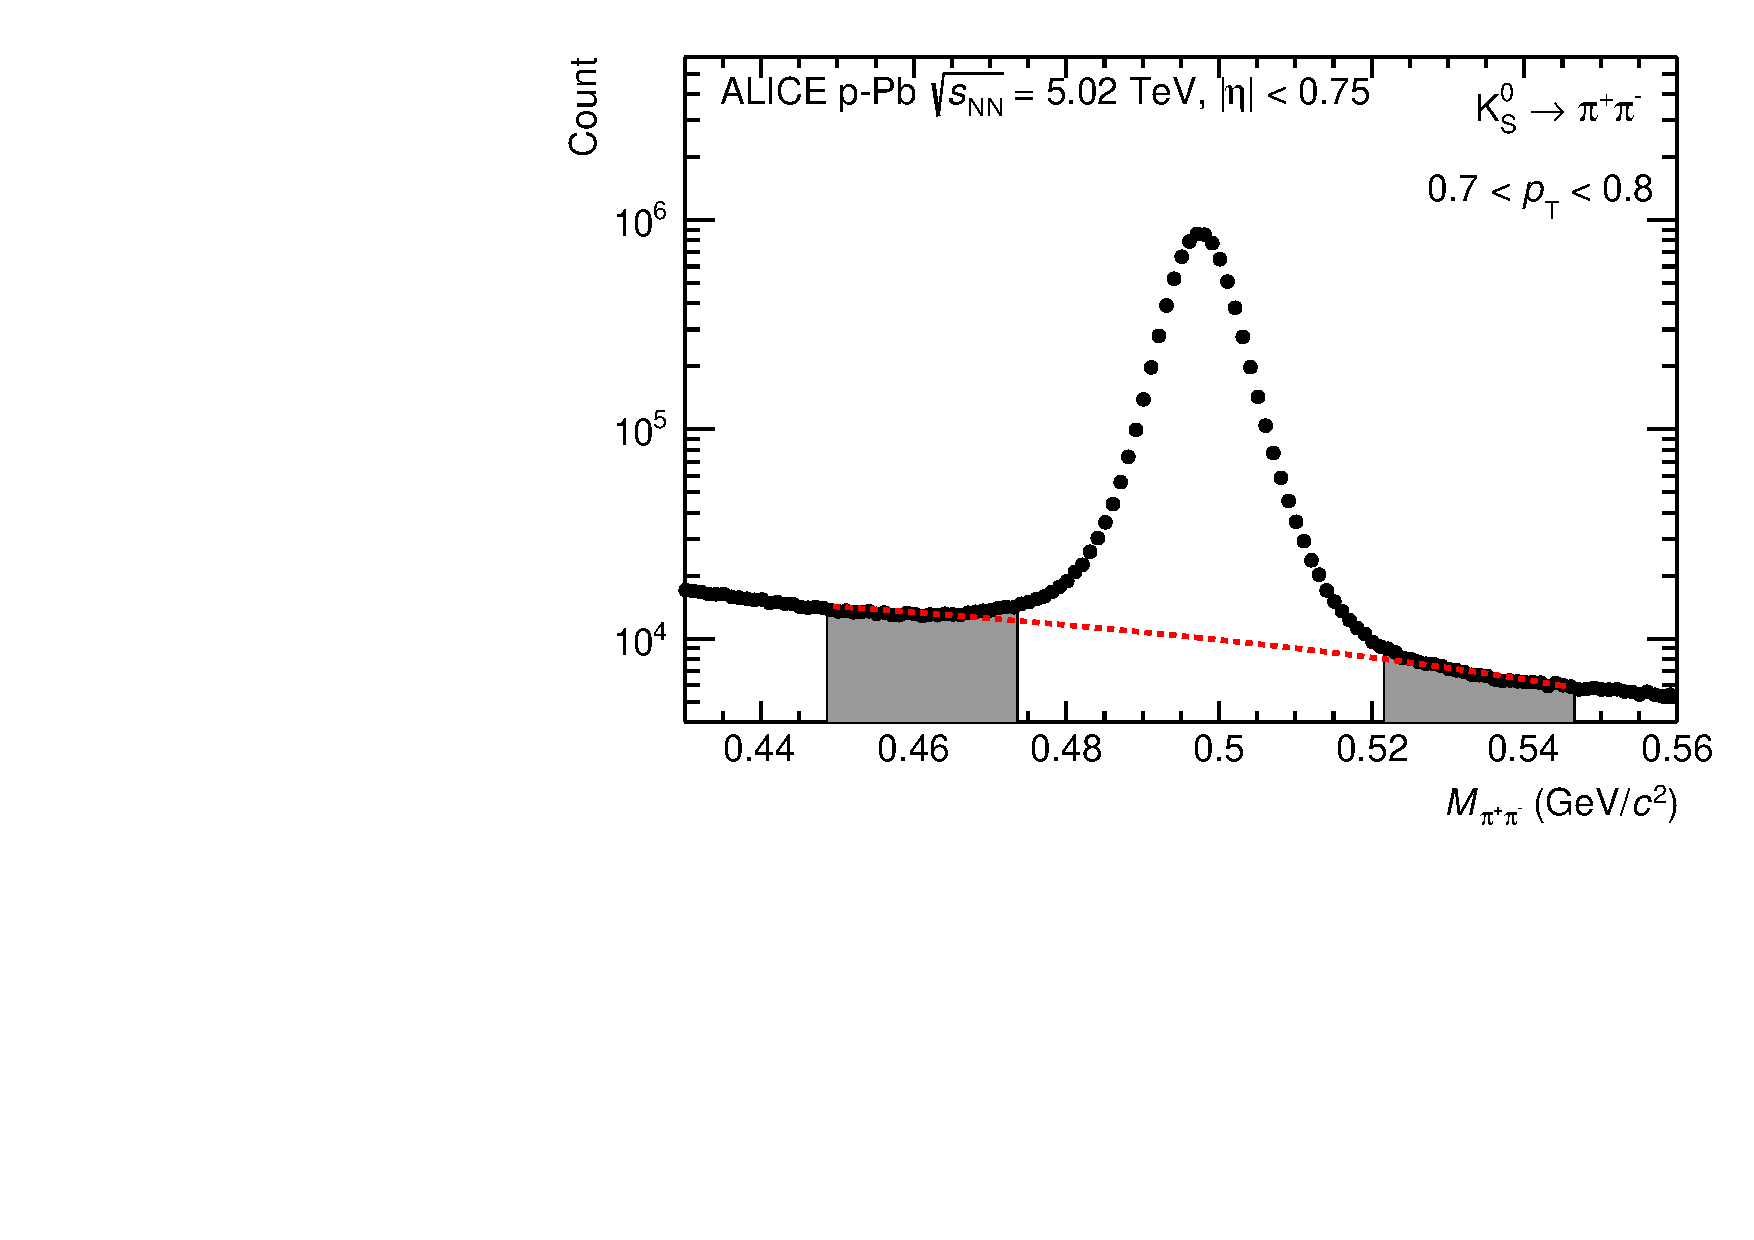
\includegraphics[width=.4\textwidth]{cf01_1}
%DIFDELCMD < 		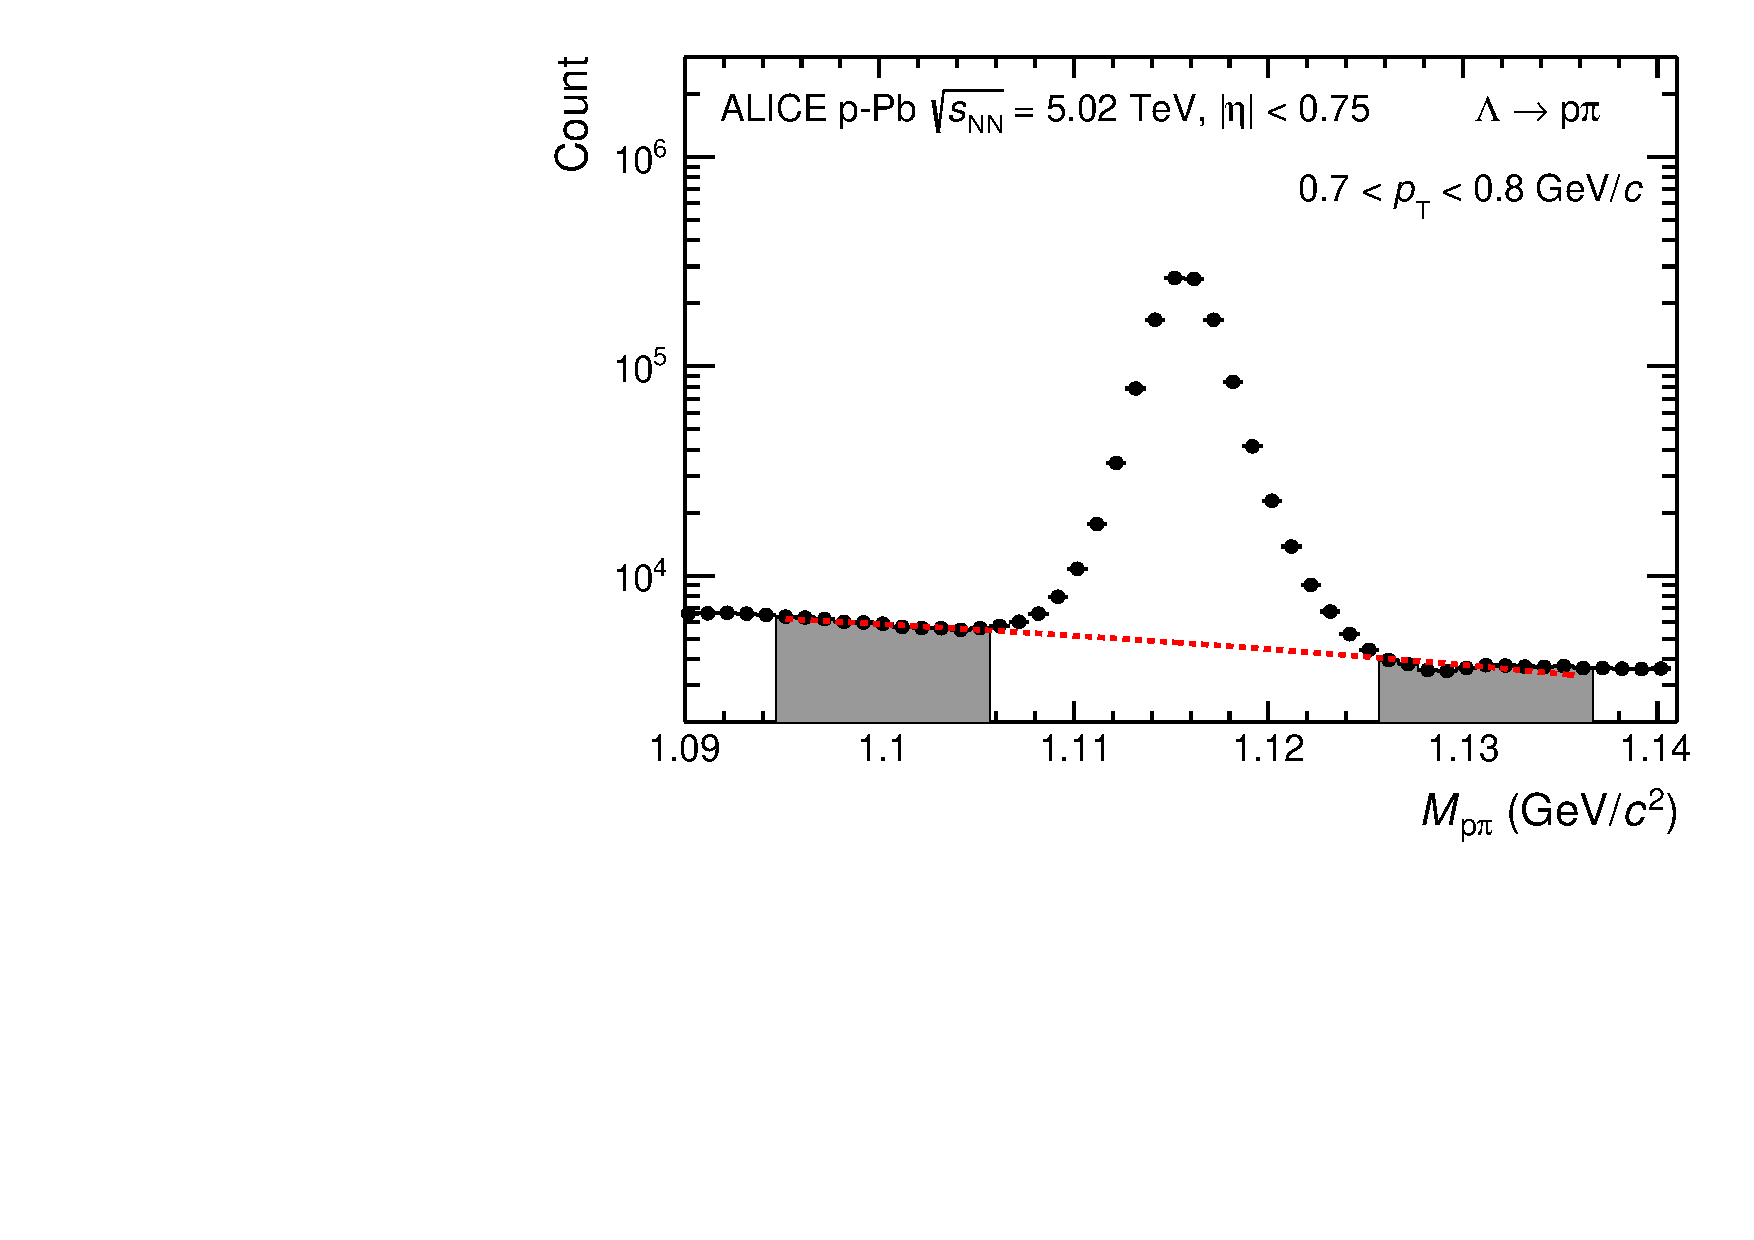
\includegraphics[width=.4\textwidth]{cf01_2}
%DIFDELCMD < 		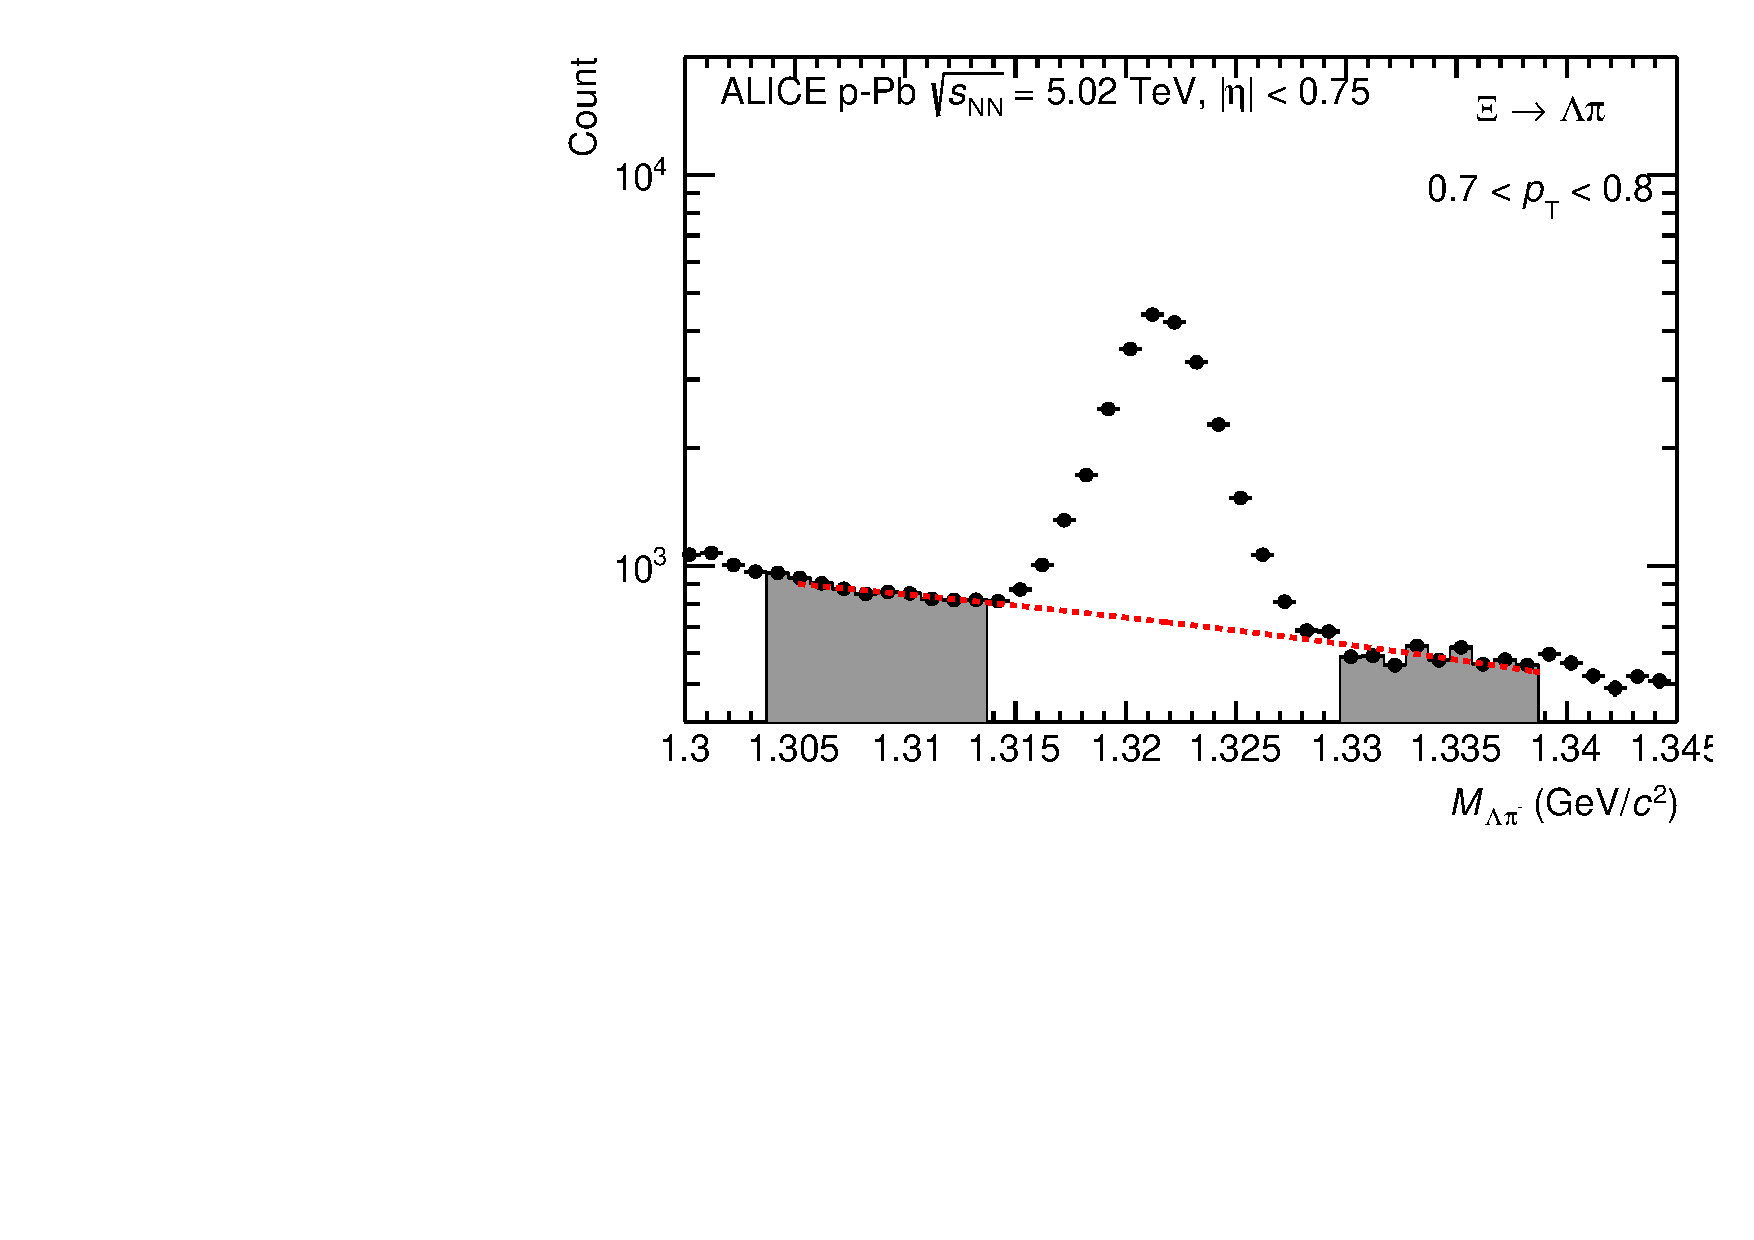
\includegraphics[width=.4\textwidth]{cf01_3}
%DIFDELCMD < 		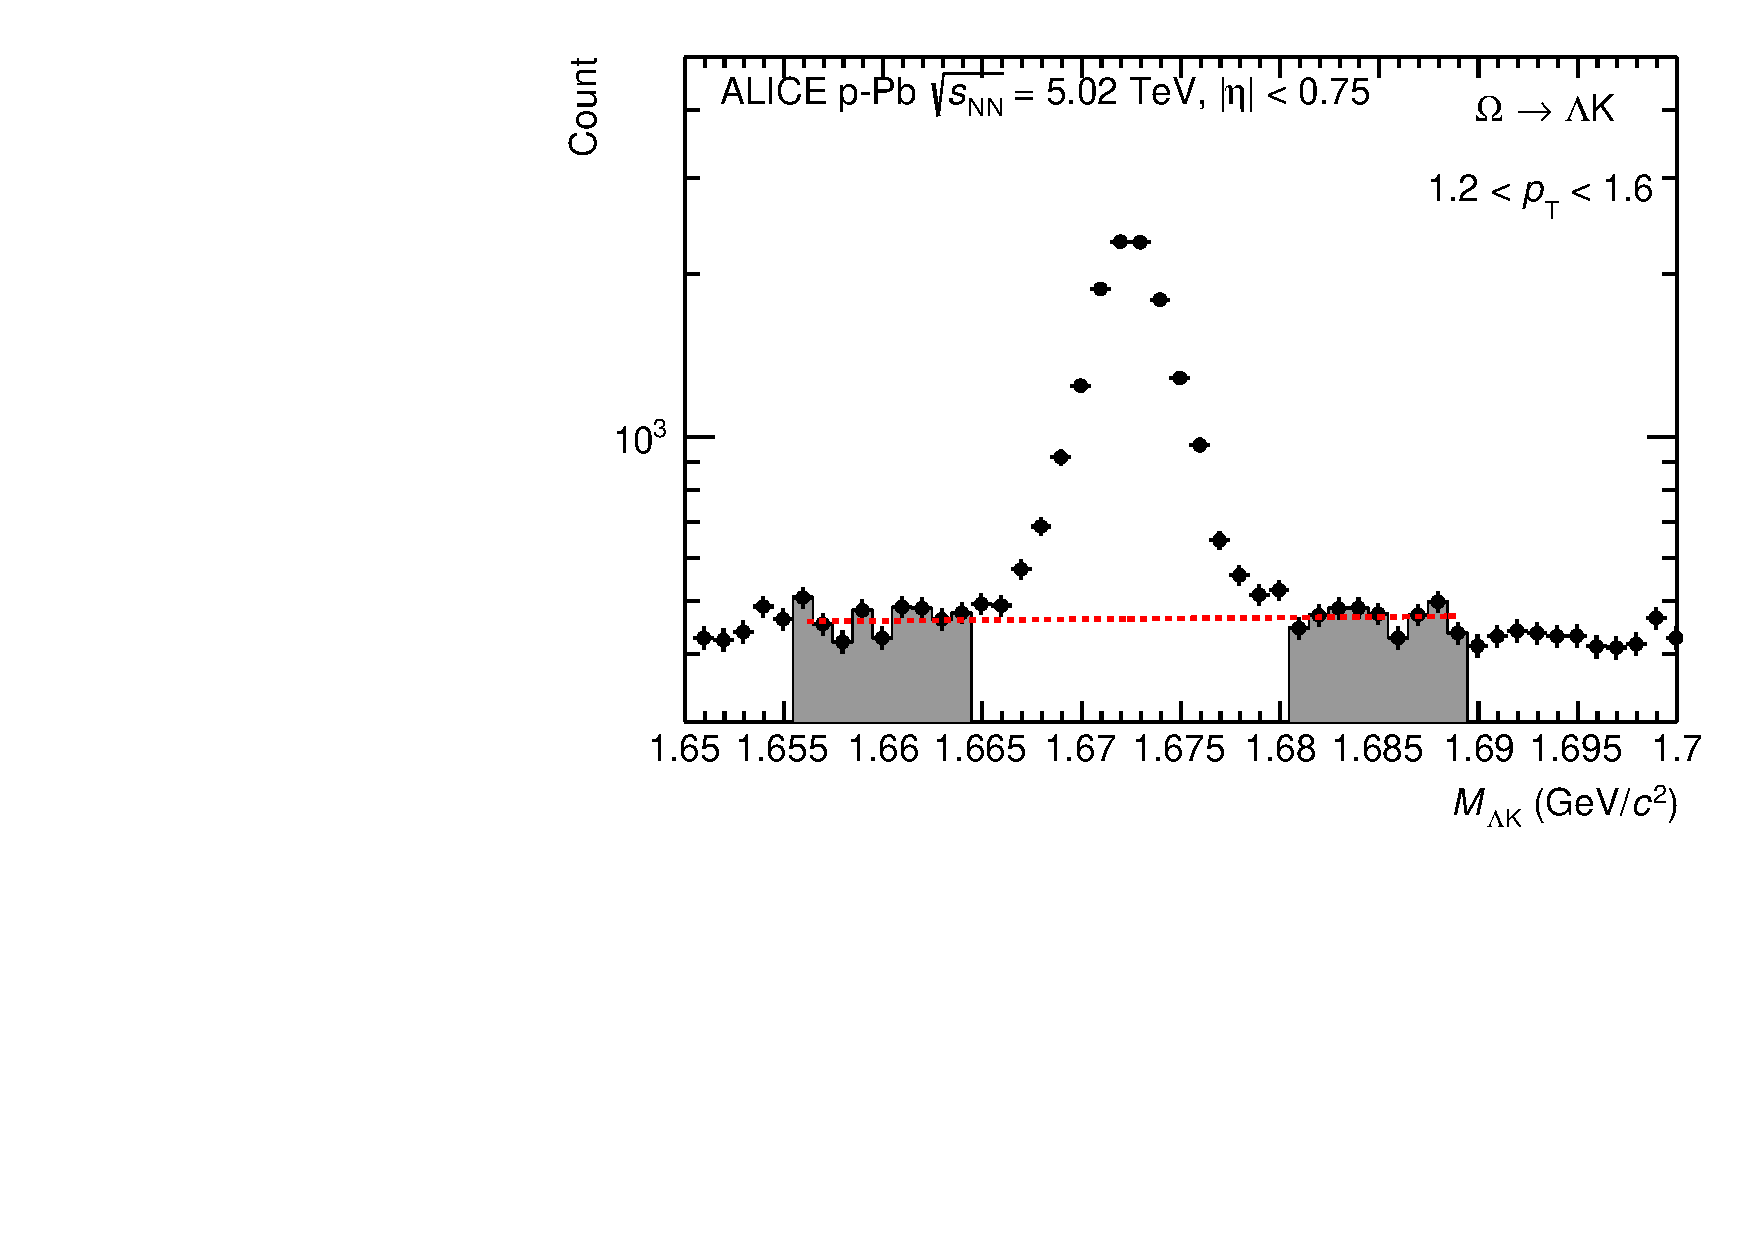
\includegraphics[width=.4\textwidth]{cf01_4}
%DIFDELCMD < 		%%%
\DIFdelendFL \DIFaddbeginFL 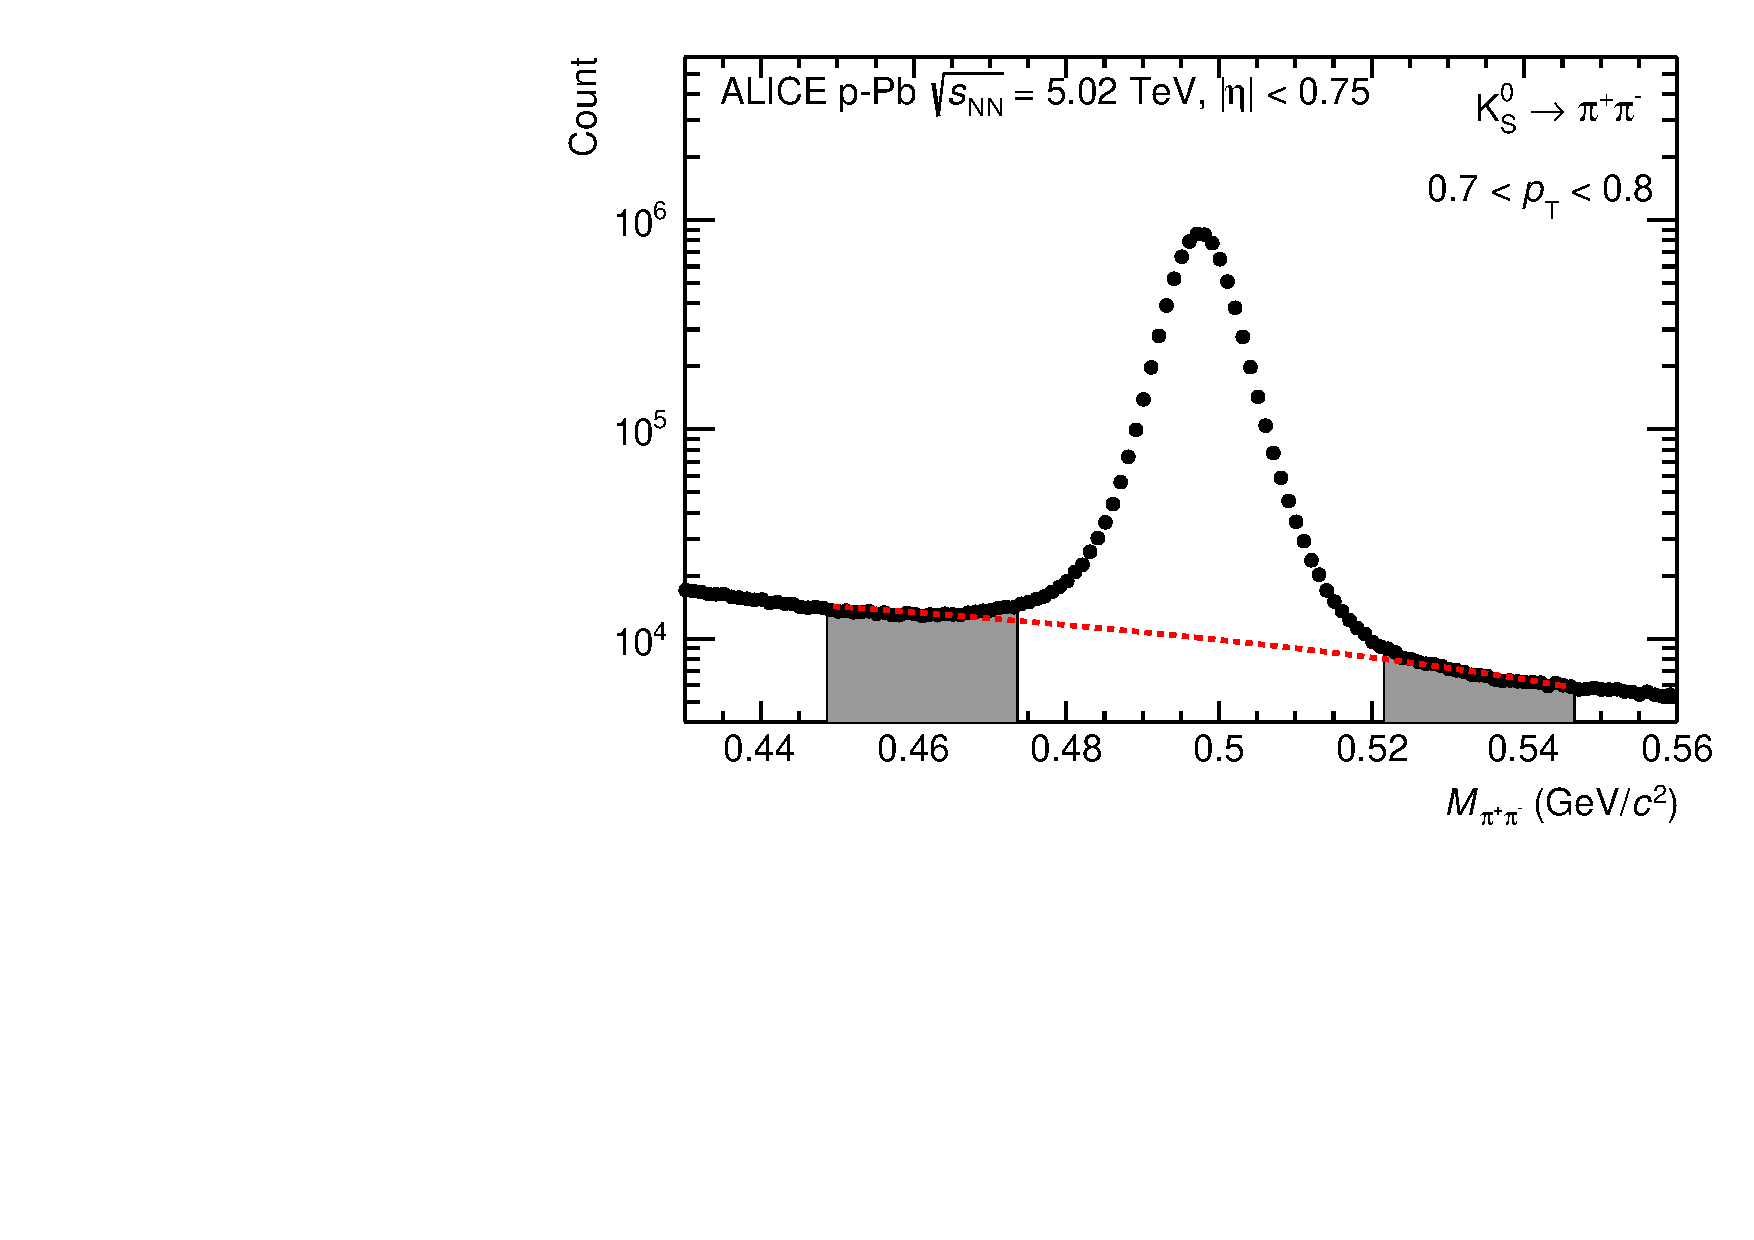
\includegraphics[width=.49\textwidth]{cf01_1}
		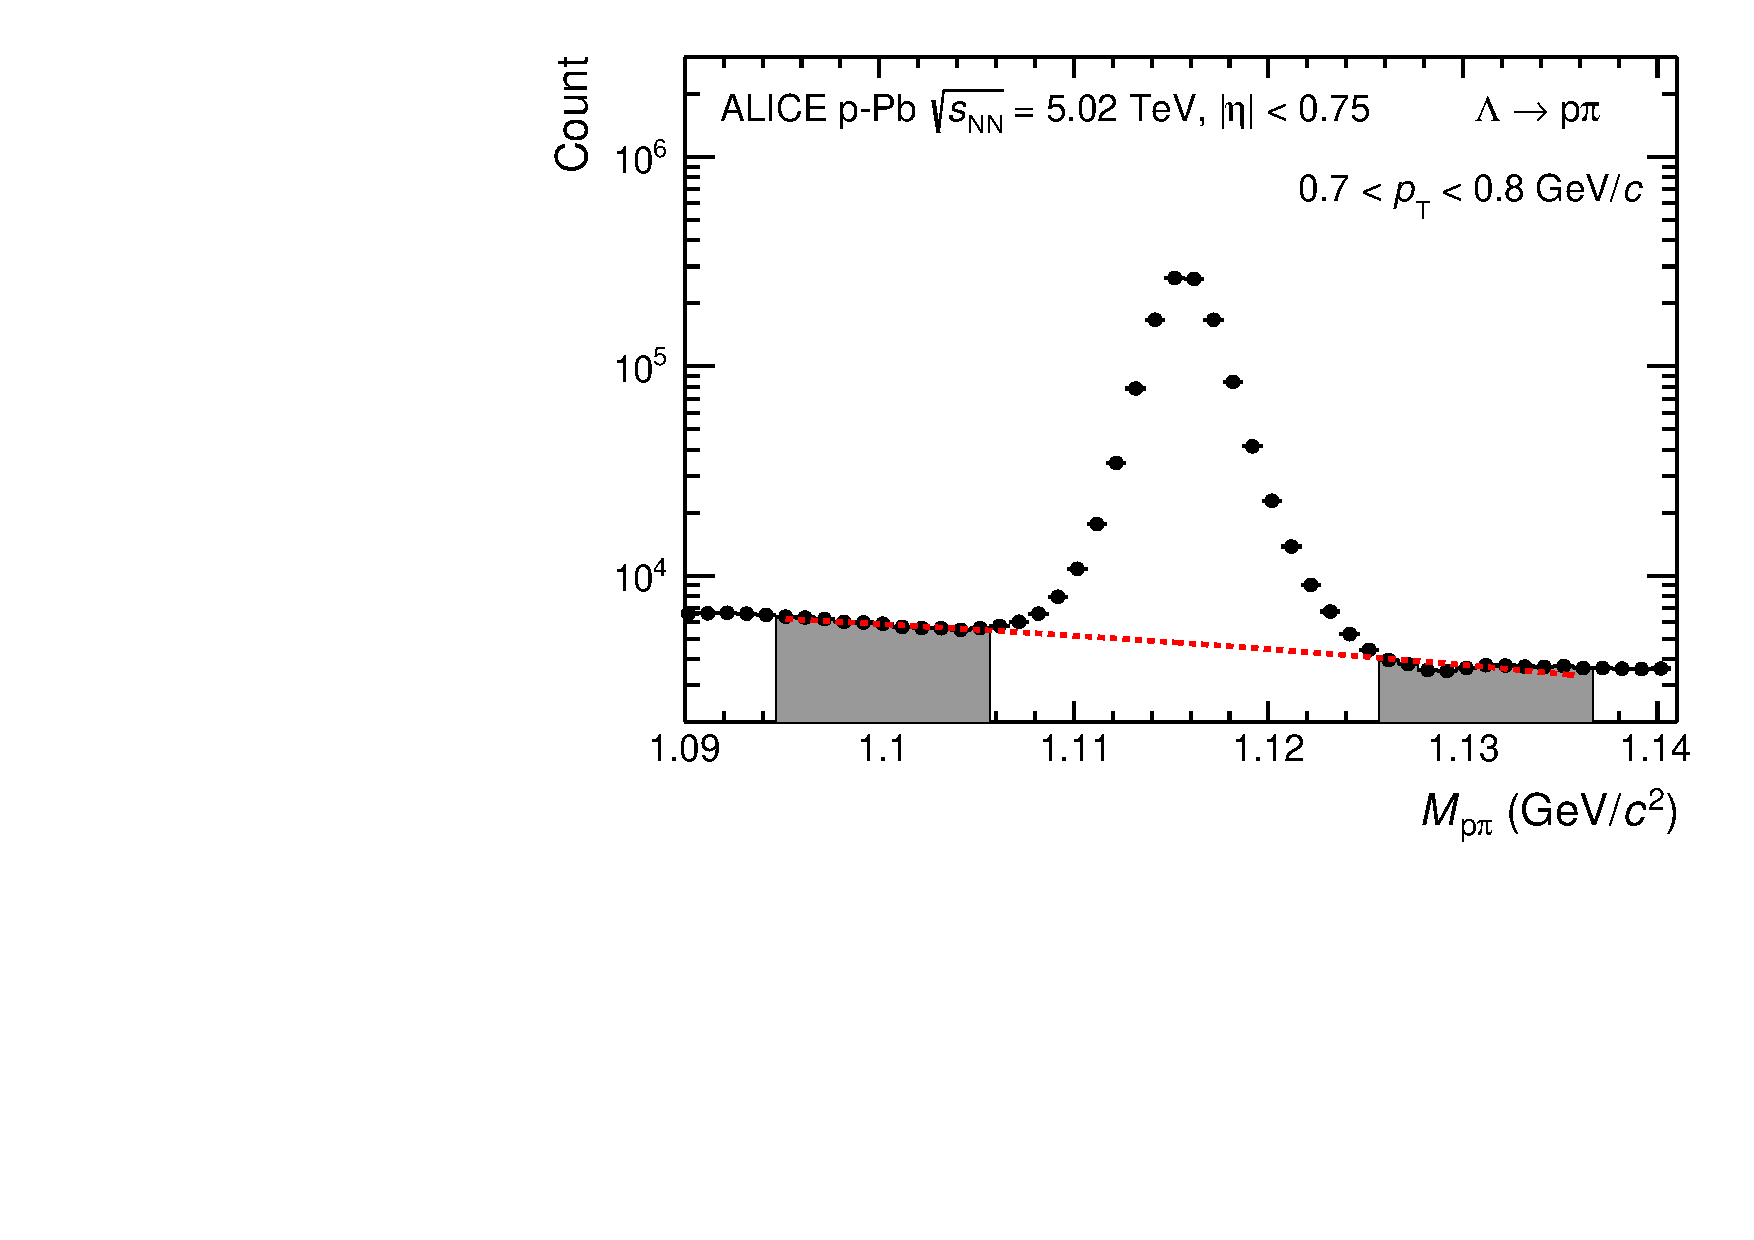
\includegraphics[width=.49\textwidth]{cf01_2}
		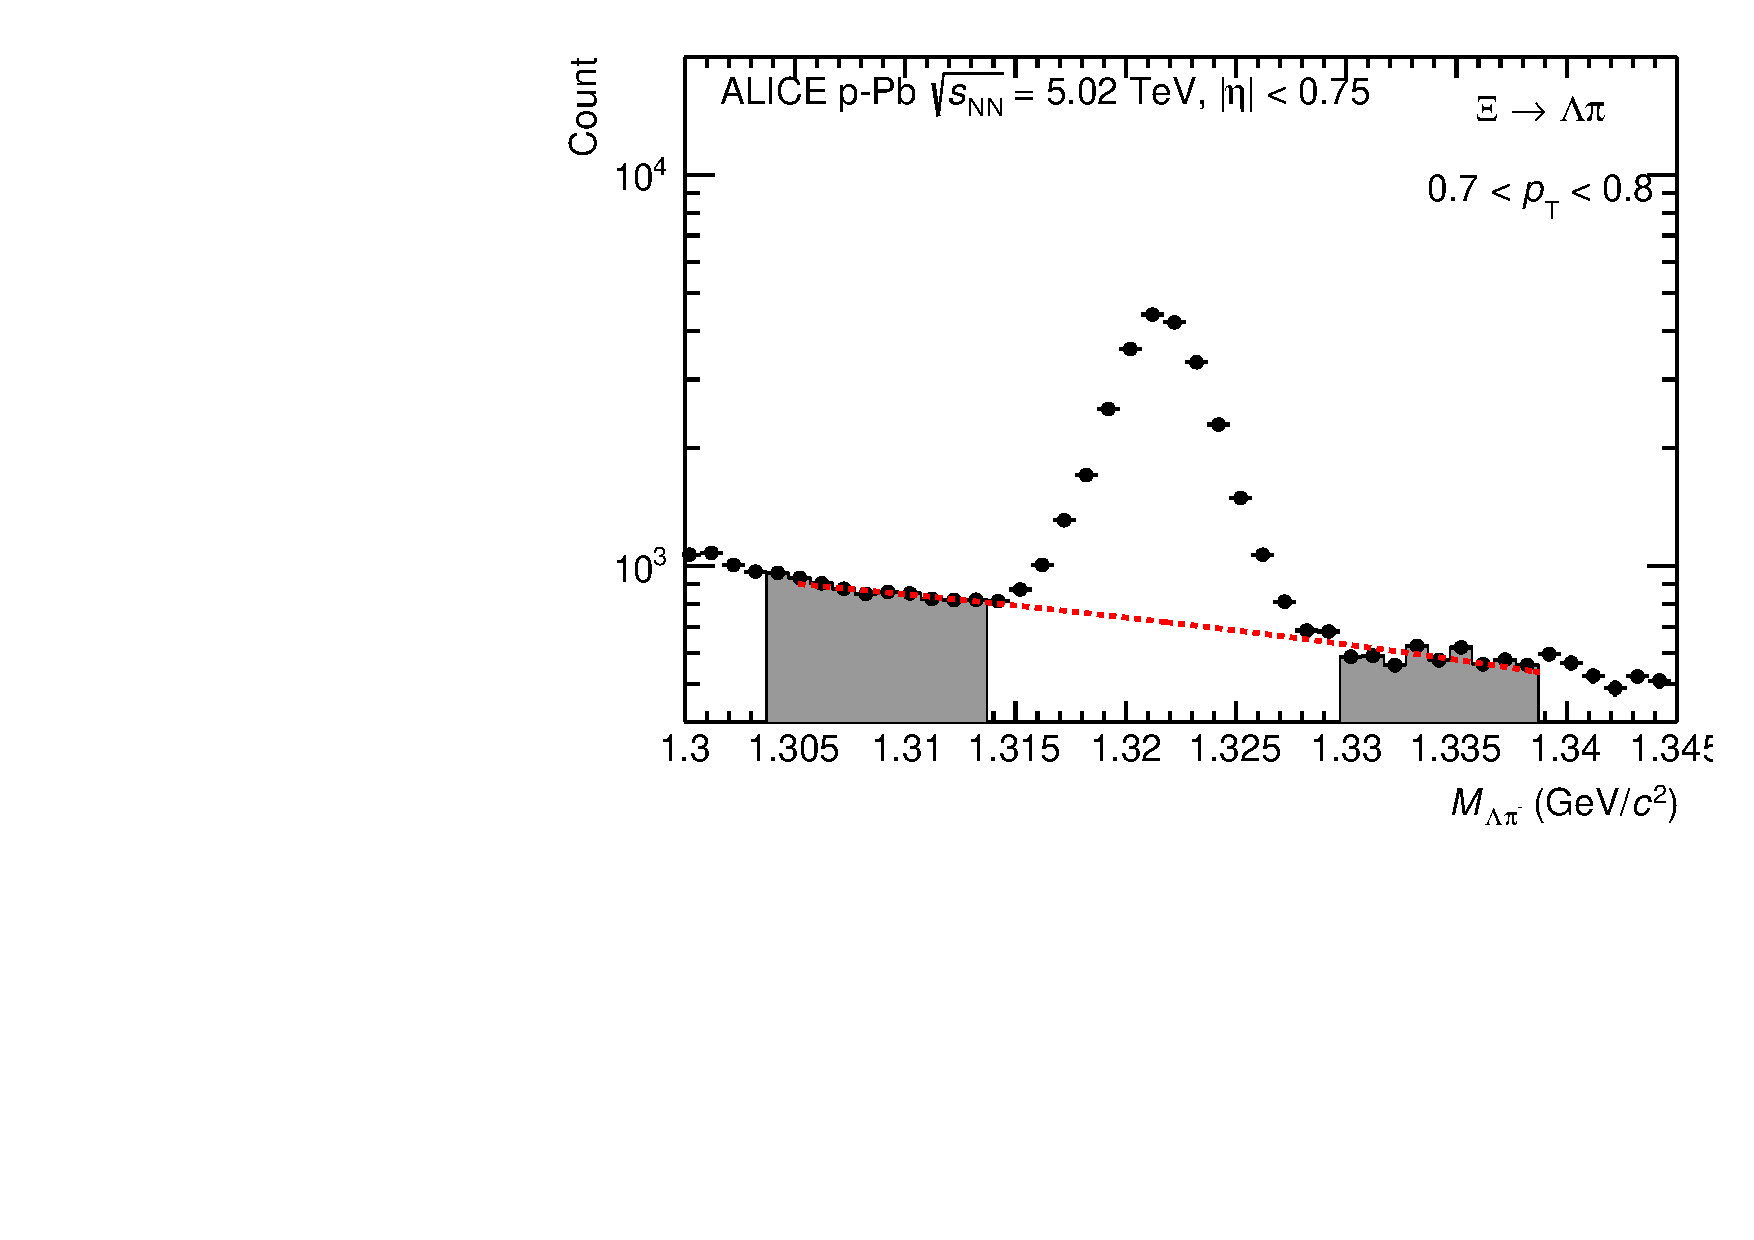
\includegraphics[width=.49\textwidth]{cf01_3}
		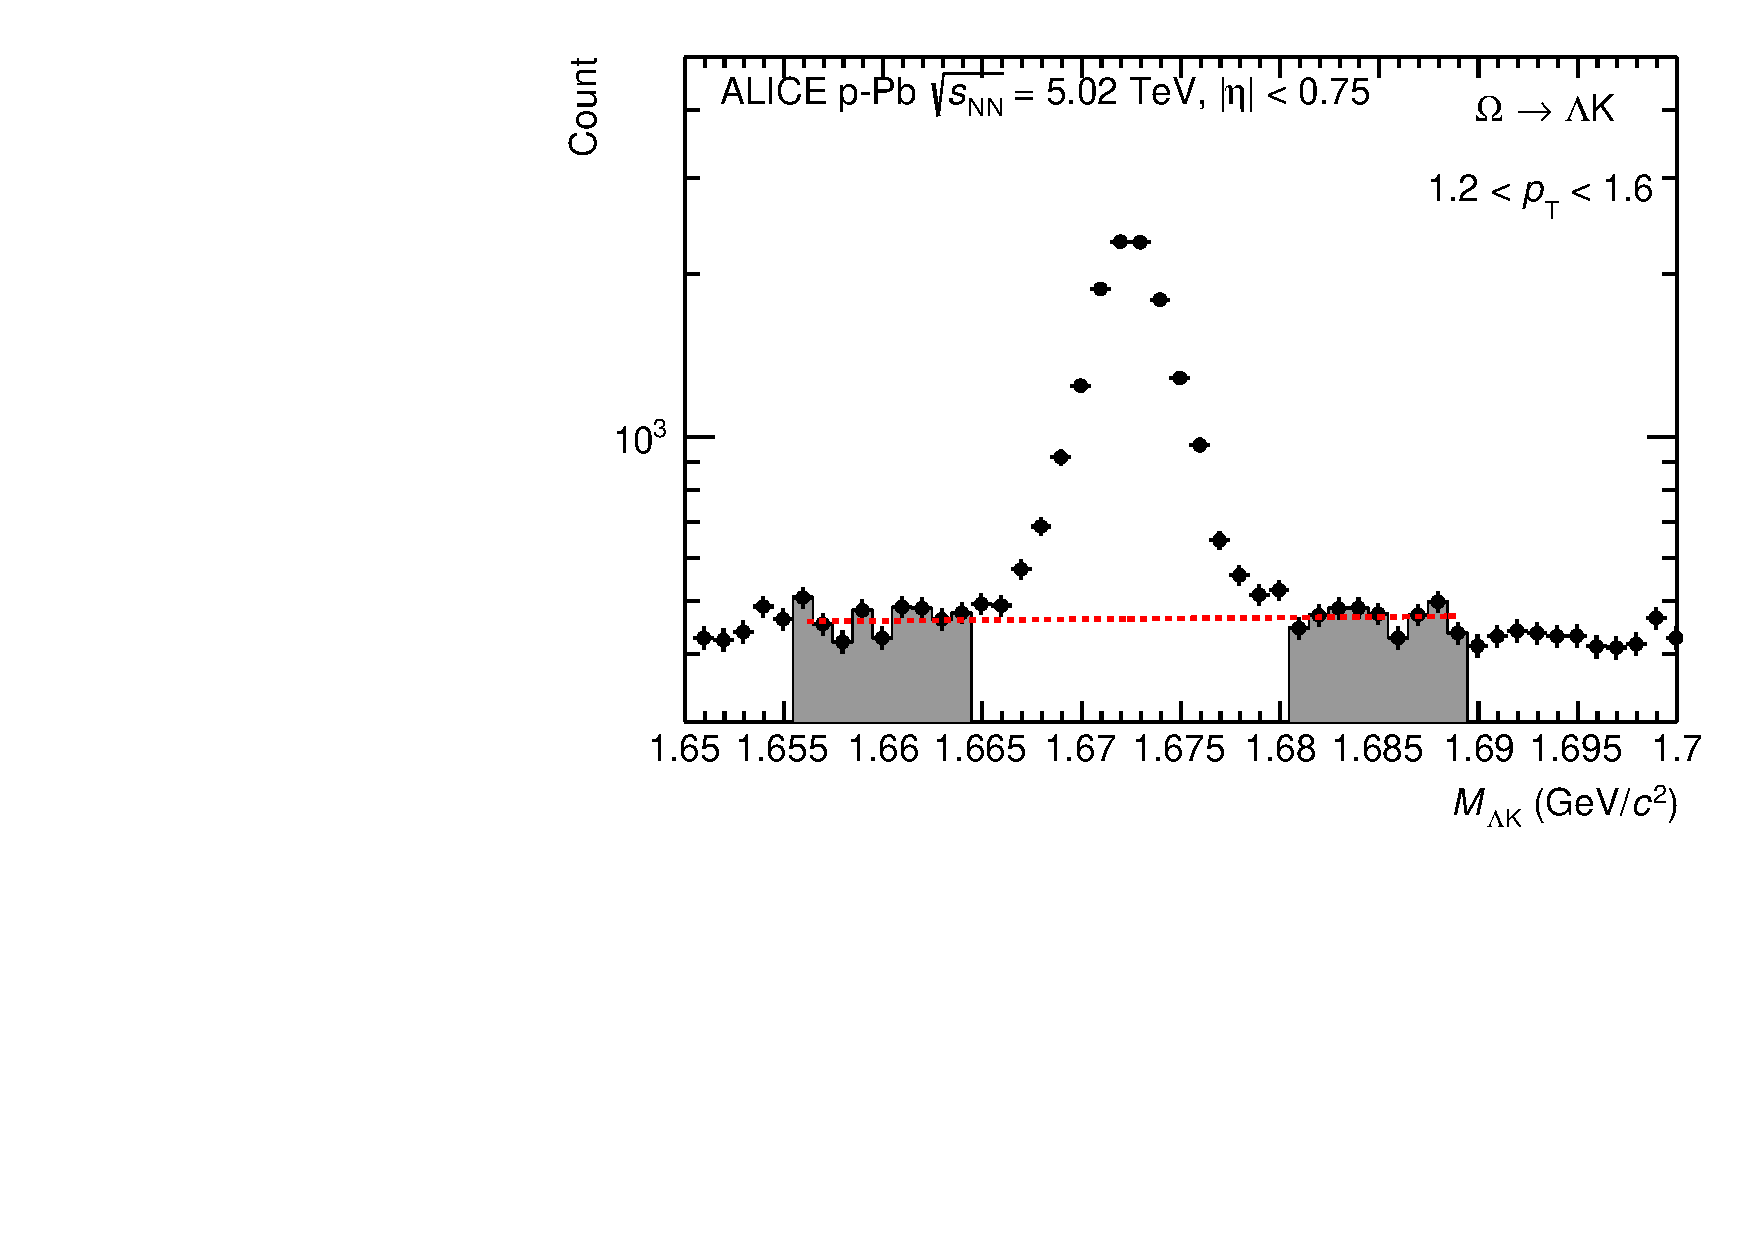
\includegraphics[width=.49\textwidth]{cf01_4}
		\DIFaddendFL \caption{Invariant \DIFdelbeginFL \DIFdelFL{Mass }\DIFdelendFL \DIFaddbeginFL \DIFaddFL{mass }\DIFaddendFL distribution for $\kzero$, $\lmb$, $\Xi$ and $\Omega$ in different $\pT$ intervals in MB \pPb \DIFdelbeginFL \DIFdelFL{system}\DIFdelendFL \DIFaddbeginFL \DIFaddFL{collisions at }\fivenn\DIFaddendFL . The candidates are reconstructed in $|\eta|<0.75$.
			The grey areas are used for \DIFaddbeginFL \DIFaddFL{background estimation applied in the }\DIFaddendFL signal extraction in the bin counting procedure.\DIFdelbeginFL \DIFdelFL{The red dashed lines represent the fit to the background distributions and the interpolate to the ``peak'' region.}\DIFdelendFL }
			%DIF > The red dashed lines represent the fit to the background distributions and the interpolation to the signal region.}
		\label{fig:InvM}
	\end{center}
\end{figure}

\subsection{Matching of strange particles to jets and underlying event}%
\label{sec:ParJetMatch}

The strategy of matching the (multi-)strange particles with jets follow those presented in earlier work~\cite{Acharya:2021oaa}.
The matching is done on a geometrical basis \DIFdelbegin \DIFdel{which presented }\DIFdelend \DIFaddbegin \DIFadd{according to the distance variable defined }\DIFaddend in Eq.~\ref{eq:DParJet}.
\begin{equation}
d(\mathrm{particle, jet}) = \sqrt{(\eta_\mathrm{particle} -\eta_{\rm jet})^{2} + (\varphi_\mathrm{particle} -\varphi_{\rm jet})^{2}}
\label{eq:DParJet}
\end{equation}
If the distance between the particle candidate and the jet ($d$) is smaller than \DIFdelbegin \DIFdel{the matching distance $D$ (}\DIFdelend \DIFaddbegin \DIFadd{a pre-defined maximum distance ($D_\mathrm{max}$ }\DIFaddend = 0.4), the candidate is considered to be inside the jet cone (JC).
The raw yields in JC are not only composed of the \DIFdelbegin \DIFdel{hadron }\DIFdelend \DIFaddbegin \DIFadd{hadrons }\DIFaddend produced via jet fragmentation (\DIFdelbegin \DIFdel{write as }\DIFdelend JE), but also \DIFdelbegin \DIFdel{hadron from Underlying Event }\DIFdelend \DIFaddbegin \DIFadd{from hadrons from the underlying event }\DIFaddend (UE) \DIFdelbegin \DIFdel{, which is }\DIFdelend defined as the sum of all particles which are not produced via hard parton fragmentation.
The UE contribution is estimated by \DIFdelbegin \DIFdel{Perpendicular Cone }\DIFdelend \DIFaddbegin \DIFadd{perpendicular cone }\DIFaddend (PC) yields.
The PC indicates the cone \DIFdelbegin \DIFdel{, which is located in }\DIFdelend \DIFaddbegin \DIFadd{in the }\DIFaddend $\eta \times \varphi$ space \DIFdelbegin \DIFdel{in }\DIFdelend \DIFaddbegin \DIFadd{located at }\DIFaddend the perpendicular direction \DIFaddbegin \DIFadd{with respect }\DIFaddend to the jet axis at the same $\eta$.
In \DIFdelbegin \DIFdel{addiction}\DIFdelend \DIFaddbegin \DIFadd{addition}\DIFaddend , the acceptance selections of inclusive (regardless of the association between \DIFaddbegin \DIFadd{the }\DIFaddend particle and hard scattering), JC and UE (multi-)strange particles are different in the $\eta$--$\varphi$ plane.
To \DIFdelbegin \DIFdel{get the particle }\DIFdelend \DIFaddbegin \DIFadd{estimate the contribution }\DIFaddend from JE the \DIFdelbegin \DIFdel{production yields are normalized to per-acceptance density (}\DIFdelend \DIFaddbegin \DIFadd{$\pT$-differential particle density (d}\DIFaddend $\rho$\DIFdelbegin \DIFdel{).
}\DIFdelend \DIFaddbegin \DIFadd{/d$\pT$) is defined in:
}\DIFaddend \begin{equation}
\DIFdelbegin %DIFDELCMD < \begin{split}
%DIFDELCMD < {\rm Inclusive:}\qquad & \frac{\dd\rho}{\dd\pT} = \frac{1}{N_{\rm ev}}\times\frac{1}{\Delta\eta\Delta\varphi}\times\frac{\dd N}{\dd\pT} \\
%DIFDELCMD < {\rm JC:}\qquad & \frac{\dd\rho}{\dd\pT} = \frac{1}{N_{\rm ev}^{\rm jet}} \times\frac{1}{\mathcal{P}_{\rm JC}\Delta\eta\Delta\varphi}\times\frac{\dd N}{\dd\pT} \\
%DIFDELCMD < {\rm PC:}\qquad & \frac{\dd\rho}{\dd\pT} = \frac{1}{N_{\rm ev}^{\rm jet}} \times\frac{1}{\mathcal{P}_{\rm PC}\Delta\eta\Delta\varphi}\times\frac{\dd N}{\dd\pT} \\
%DIFDELCMD < \end{split}
%DIFDELCMD < %%%
\DIFdelend \DIFaddbegin \begin{split}
{\rm Inclusive:}\qquad & \frac{\dd\rho}{\dd\pT} = \frac{1}{N_{\rm ev}}\times\frac{1}{\Delta\eta\Delta\varphi}\times\frac{\dd N}{\dd\pT}, \\
{\rm JC:}\qquad & \frac{\dd\rho}{\dd\pT} = \frac{1}{N_{\rm ev}^{\rm jet}} \times\frac{1}{A_{\rm jet}}\times\frac{\dd N}{\dd\pT}, \\
{\rm PC:}\qquad & \frac{\dd\rho}{\dd\pT} = \frac{1}{N_{\rm ev}^{\rm jet}} \times\frac{1}{A_{\rm PC}}\times\frac{\dd N}{\dd\pT}. \\
\end{split}
\DIFaddend \label{eq:normalize}
\end{equation}
\DIFdelbegin \DIFdel{where the $\mathcal{P}$ denotes the probability of particles in a given selection found in the $\eta$--$\varphi$ plane with respect to the inclusive one.
}\DIFdelend %DIF > \begin{equation}
%DIF > \begin{split}
%DIF > {\rm Inclusive:}\qquad & \frac{\dd\rho}{\dd\pT} = \frac{1}{N_{\rm ev}}\times\frac{1}{\Delta\eta\Delta\varphi}\times\frac{\dd N}{\dd\pT}, \\
%DIF > {\rm JC:}\qquad & \frac{\dd\rho}{\dd\pT} = \frac{1}{N_{\rm ev}^{\rm jet}} \times\frac{1}{\mathcal{P}_{\rm JC}\Delta\eta\Delta\varphi}\times\frac{\dd N}{\dd\pT}, \\
%DIF > {\rm PC:}\qquad & \frac{\dd\rho}{\dd\pT} = \frac{1}{N_{\rm ev}^{\rm jet}} \times\frac{1}{\mathcal{P}_{\rm PC}\Delta\eta\Delta\varphi}\times\frac{\dd N}{\dd\pT}. \\
%DIF > \end{split}
%DIF > \label{eq:normalize}
%DIF > \end{equation}
\DIFaddbegin \DIFadd{Where the $\Delta\eta\Delta\varphi$ is the acceptance in pseudo-rapidity and azimuthal angle, the $A_\mathrm{jet}$ is the jet area, and the $A_\mathrm{PC}$ is the perpendicular cone area.
The density of particles within jet (JE) can be defined as:
}\begin{equation}
\DIFadd{\label{eq:je}
	}{\DIFadd{\rm JE = JC - PC}}\DIFadd{.
}\end{equation}
\DIFaddend 

\subsection{Corrections for strange particles reconstruction and feed-down}
\label{SubSec:Correction}
The reconstruction efficiency of \DIFdelbegin \DIFdel{particles are obtained in }\DIFdelend \DIFaddbegin \DIFadd{each particle is obtained from }\DIFaddend Monte Carlo simulated data.
\DIFdelbegin \DIFdel{These are estimated using }\DIFdelend \DIFaddbegin \DIFadd{For this purpose }\DIFaddend PYTHIA 8.2~\cite{Sjostrand:2014zea} and DPMJet~\cite{Roesler:2000he} \DIFdelbegin \DIFdel{generators }\DIFdelend in \pp and \pPb \DIFdelbegin \DIFdel{, respectively, and tracsported through a }\DIFdelend \DIFaddbegin \DIFadd{collisions are used and the simulated data are propagated through the detector by }\DIFaddend GEANT 3~\cite{Brun:1994aa} \DIFaddbegin \DIFadd{to simulate ALICE detector response}\DIFaddend .
Due to \DIFdelbegin \DIFdel{different $\eta$-shape between particle in JC and the inclusive one, it is needed to take the $\eta$ dependence of different particle distributions into account}\DIFdelend \DIFaddbegin \DIFadd{differences in the experimental acceptance for particles associated with jets and underlying event, the efficiencies of particles are estimated separately for every case}\DIFaddend ~\cite{Acharya:2021oaa}.
Fig.~\ref{fig:EffiJCIncl} shows the difference of reconstruction efficiency of JC \DIFdelbegin \DIFdel{particles }\DIFdelend \DIFaddbegin \DIFadd{particle yields }\DIFaddend and the inclusive one.
\begin{figure}[!ht]
	\begin{center}
		\DIFdelbeginFL %DIFDELCMD < 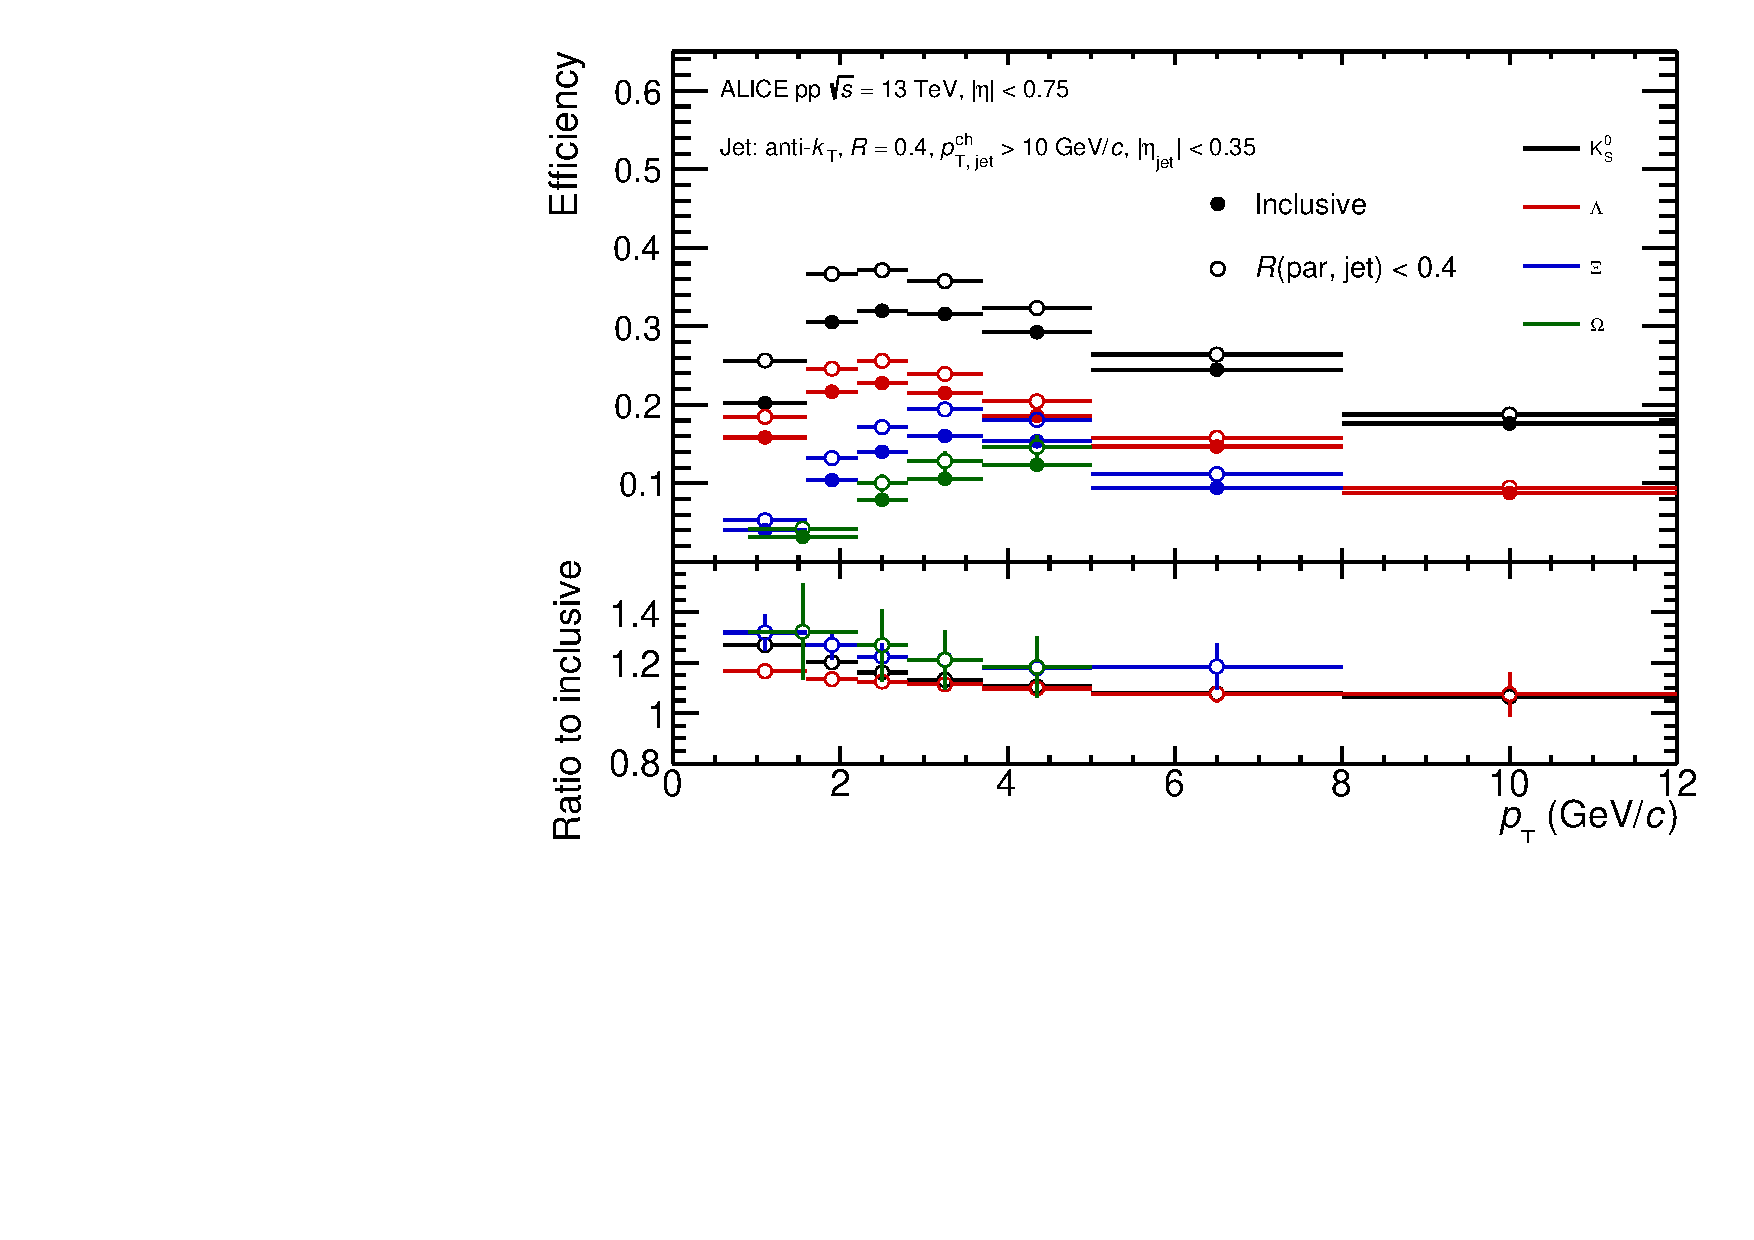
\includegraphics[width=.4\textwidth]{cf02_1}
%DIFDELCMD < 		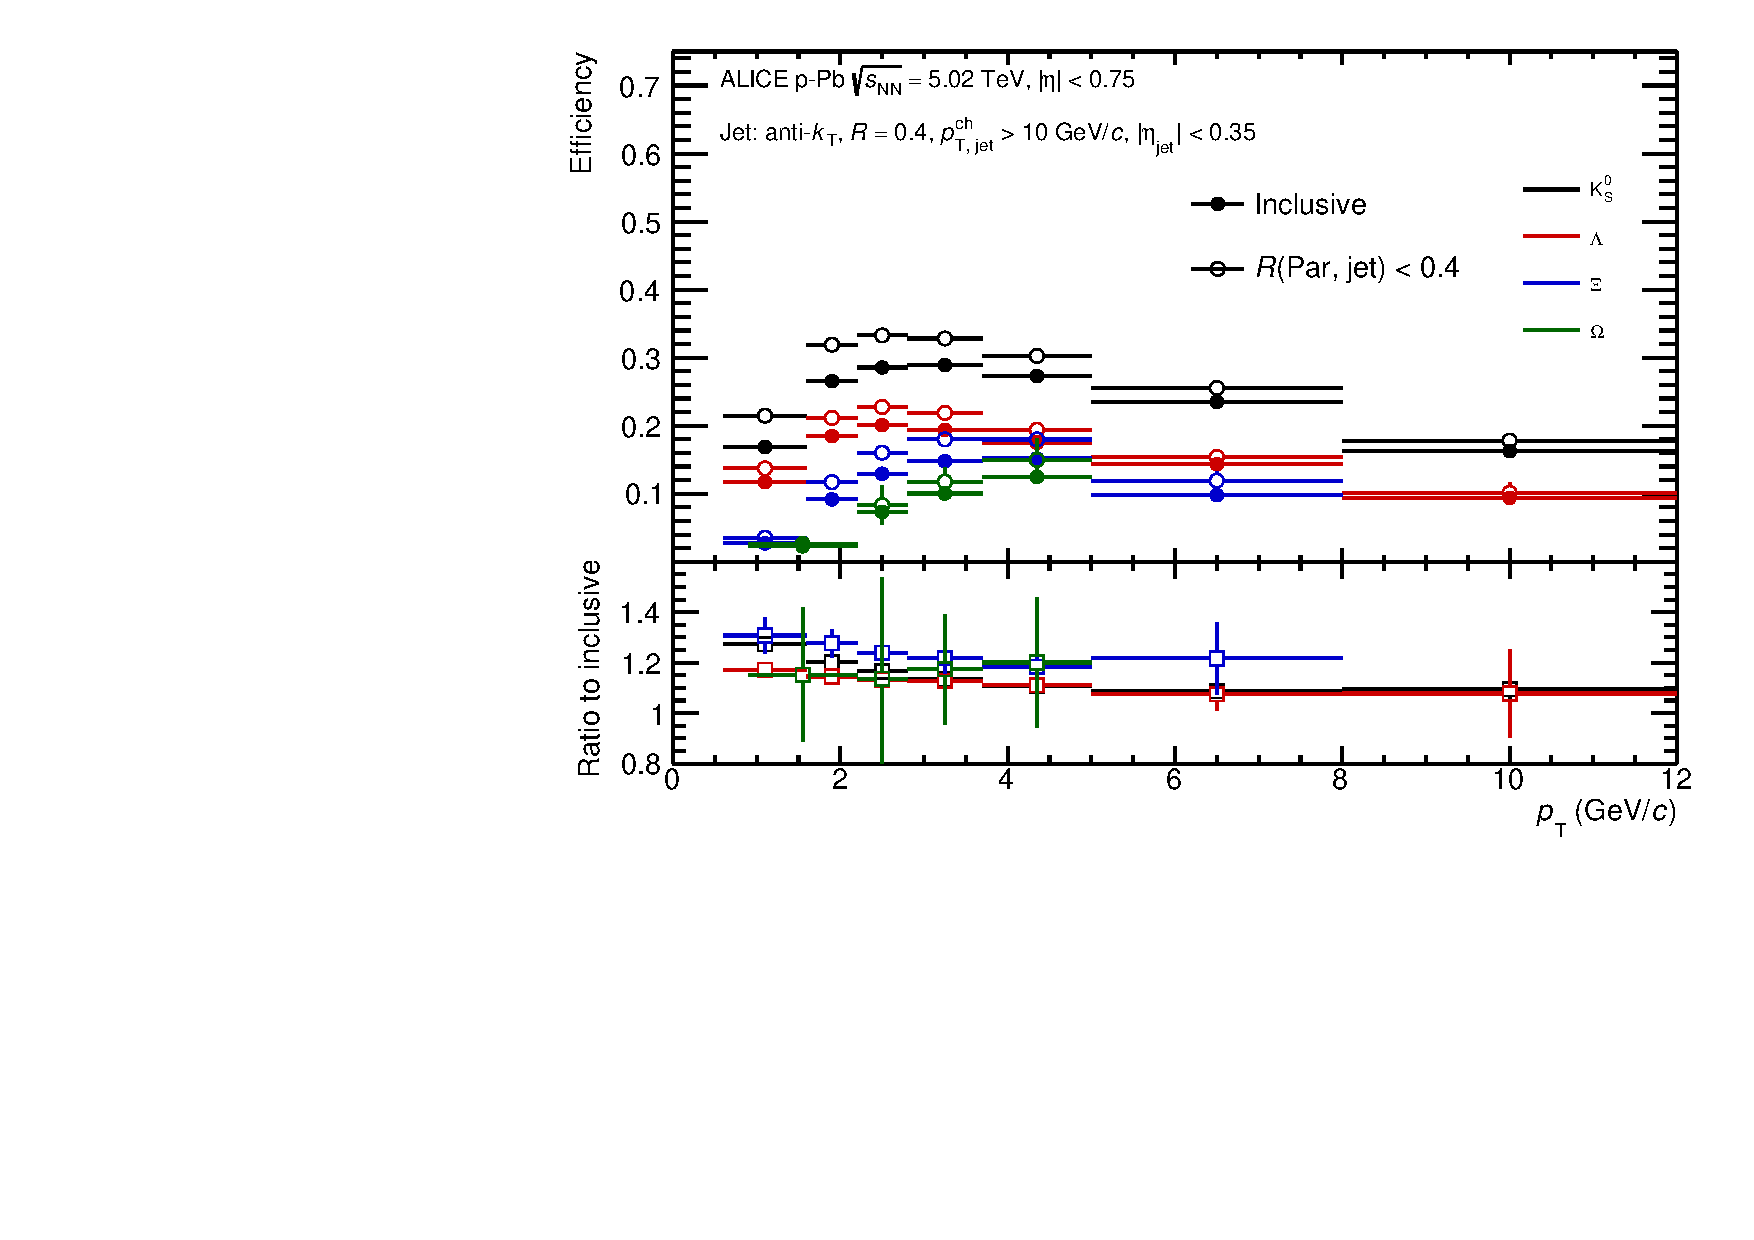
\includegraphics[width=.4\textwidth]{cf02_2}
%DIFDELCMD < 	%%%
\DIFdelendFL \DIFaddbeginFL 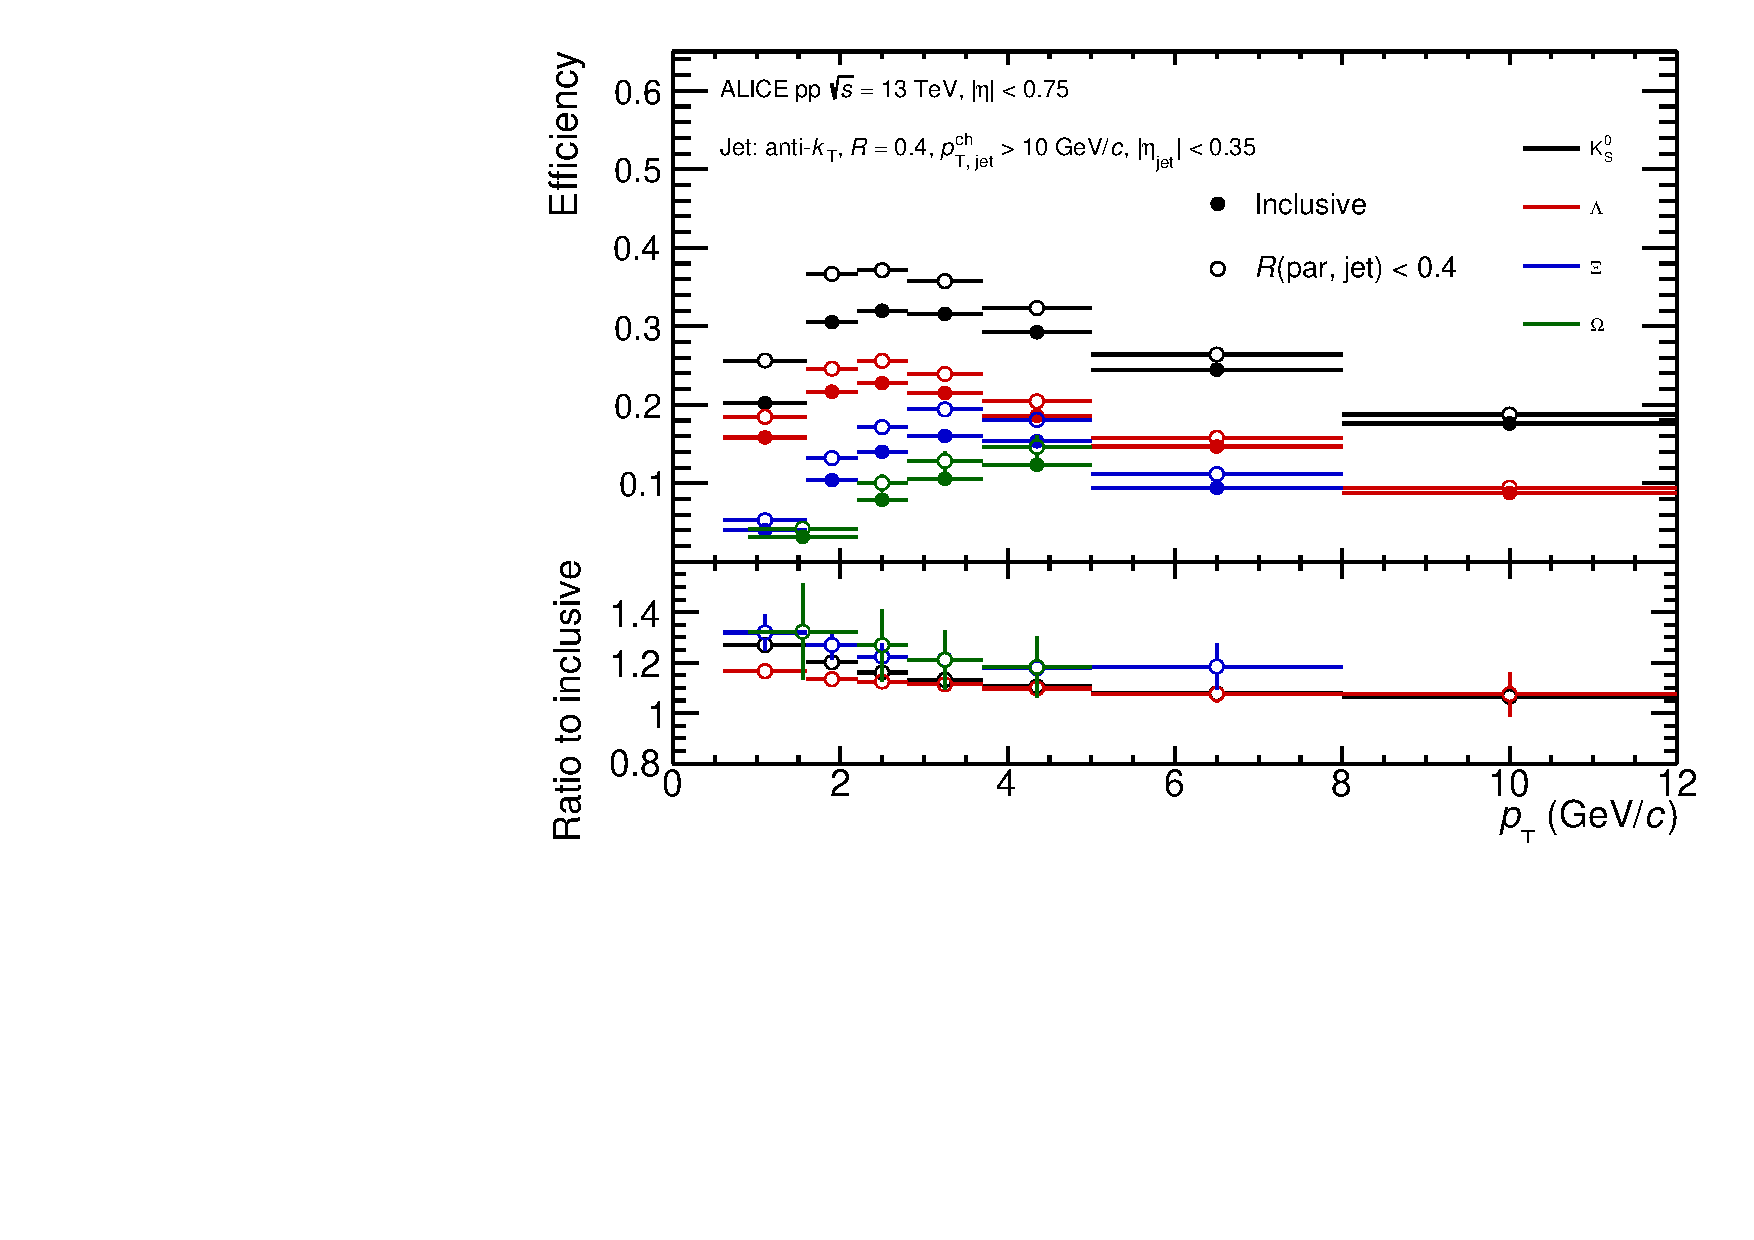
\includegraphics[width=.49\textwidth]{cf02_1}
		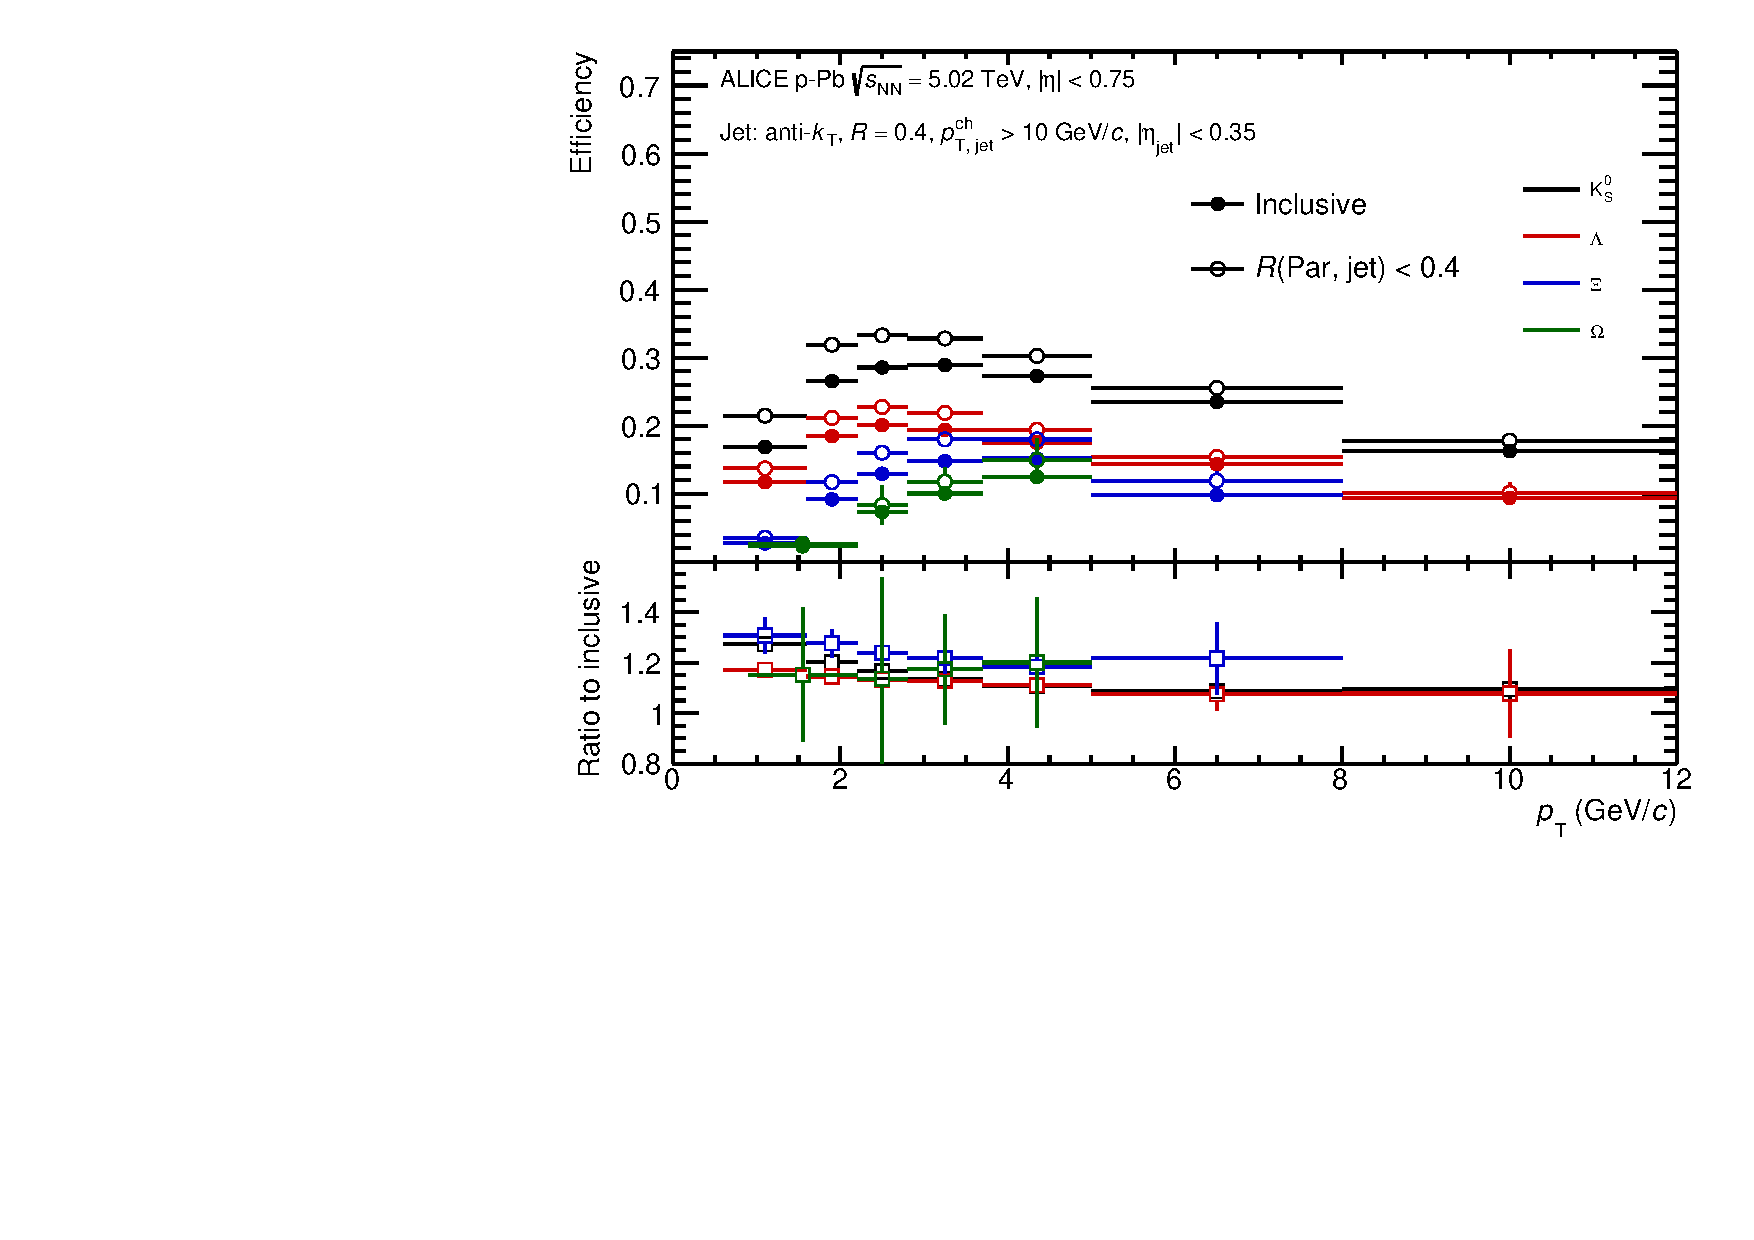
\includegraphics[width=.49\textwidth]{cf02_2}
	\DIFaddendFL \end{center}
	\caption{\DIFdelbeginFL \DIFdelFL{The }\DIFdelendFL \DIFaddbeginFL \DIFaddFL{Strange particle }\DIFaddendFL reconstruction efficiency \DIFdelbeginFL \DIFdelFL{for the particles }\DIFdelendFL in \pp collisions at \thirteen (left) and in \pPb collisions at \fivenn (right) for two selections: inside jet cone, \DIFdelbeginFL \DIFdelFL{$R(\mathrm{particle, jet}) < 0.4$ }\DIFdelendFL \DIFaddbeginFL \DIFaddFL{$R(\mathrm{par, jet}) < 0.4$ }\DIFaddendFL and the inclusive one.}
	\label{fig:EffiJCIncl}
\end{figure}

Only the yields for $\lmb$ and $\almb$ are significantly affected by secondary particles coming from the decays of charged and neutral $\Xi$ baryons.
The feed-down fraction is calculated with a data-driven approach~\cite{Abelev:2013haa}.
The detailed of inclusive feed-down method \DIFdelbegin \DIFdel{has }\DIFdelend \DIFaddbegin \DIFadd{have }\DIFaddend been introduced in previous ALICE \DIFdelbegin \DIFdel{analysis works}\DIFdelend \DIFaddbegin \DIFadd{analyses}\DIFaddend ~\cite{Acharya:2019kyh, Acharya:2020uxl, ALICE:2017jyt}.
In particular, the $\lmb$ and $\almb$ in jet and UE feed-down component \DIFaddbegin \DIFadd{is }\DIFaddend usually estimated by inclusive $\Xis$ spectra and PYTHIA simulations~\cite{Acharya:2021oaa}, due to lack of $\Xis$ in jet and UE results.
In this work, the feed-down fraction in jets and UE is computed for each $\pT$ bin by the measured $\Xis$ in jets and UE spectra, thereby assuming that the production rates of charged and neutral $\Xi$ are equal.
Figure~\ref{fig:FdFrac} shows the results of feed-down fraction in JC and the inclusive one.
\begin{figure}[!ht]
	\begin{center}
		\DIFdelbeginFL %DIFDELCMD < 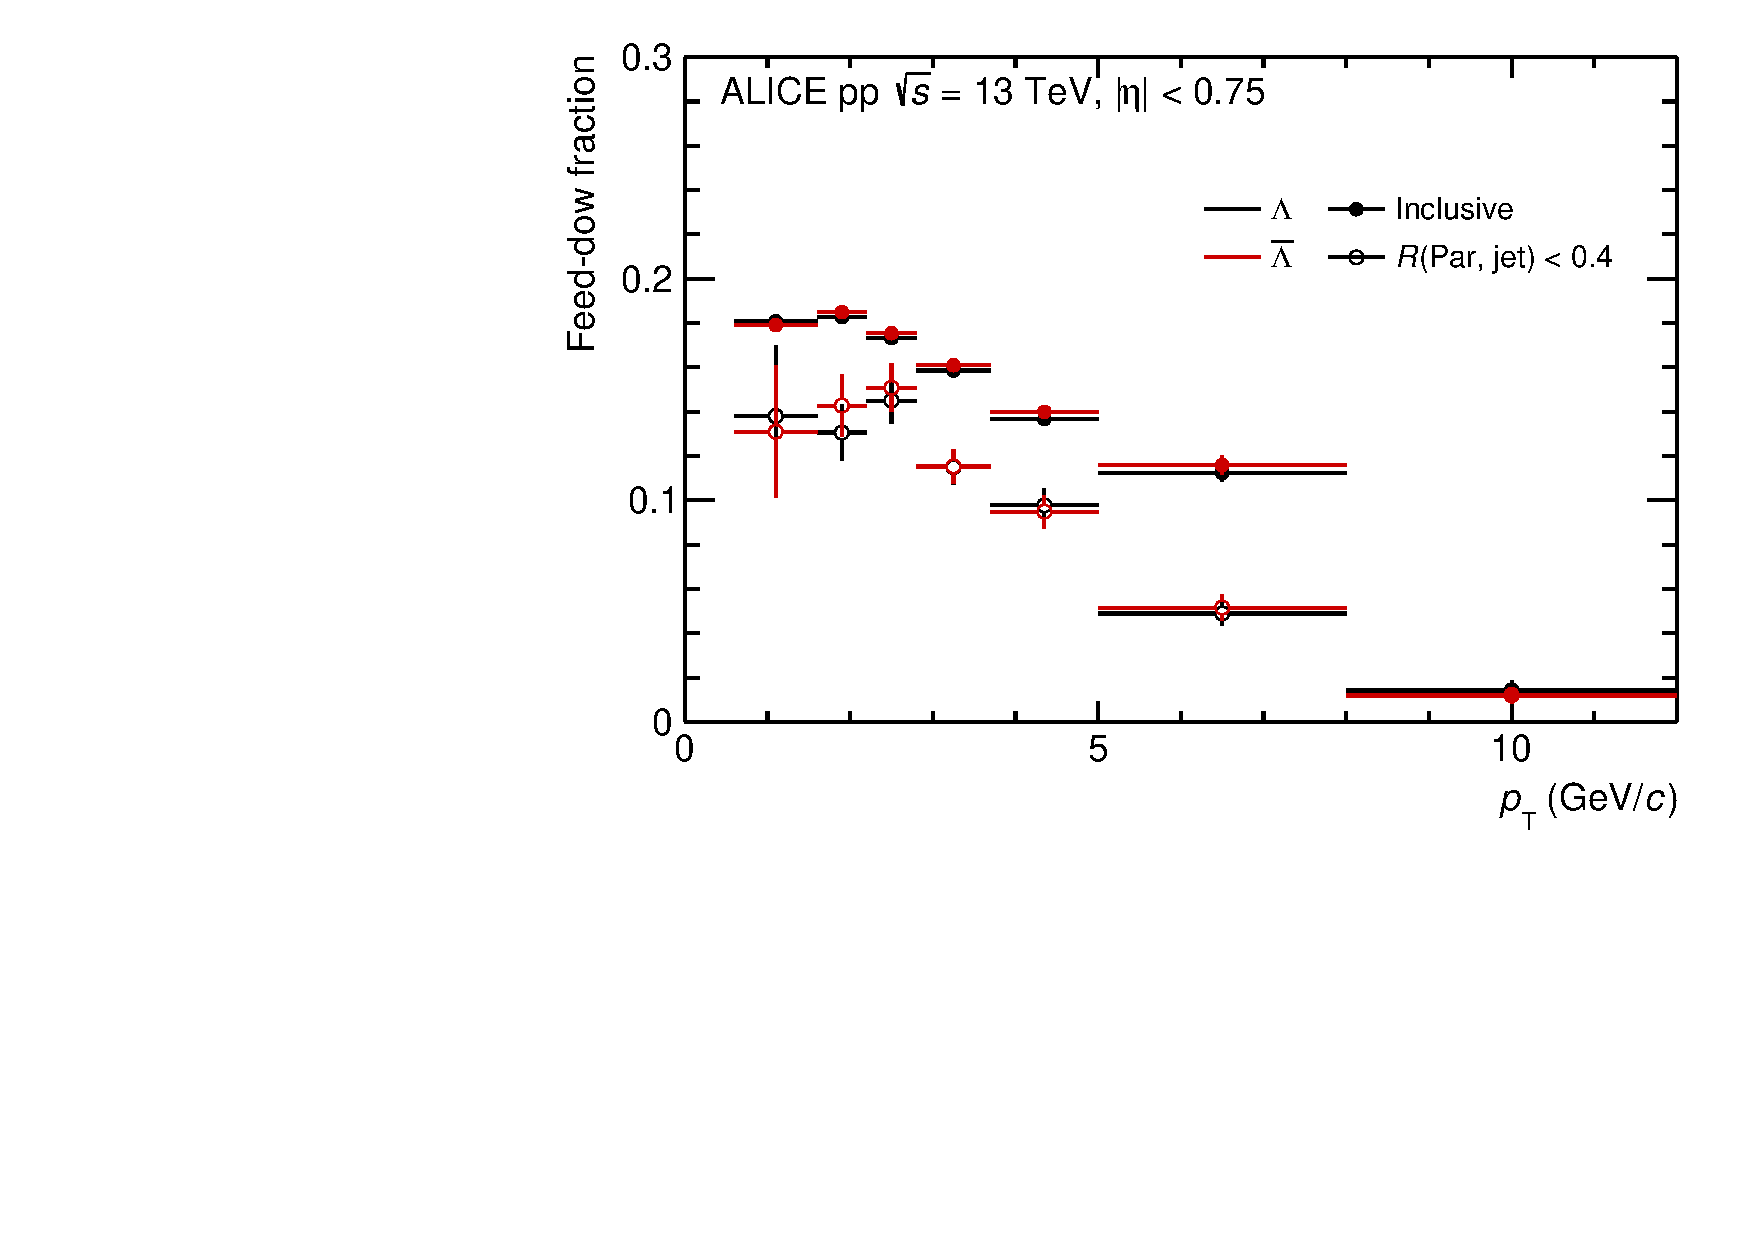
\includegraphics[width=.4\textwidth]{cf03_1}
%DIFDELCMD < 		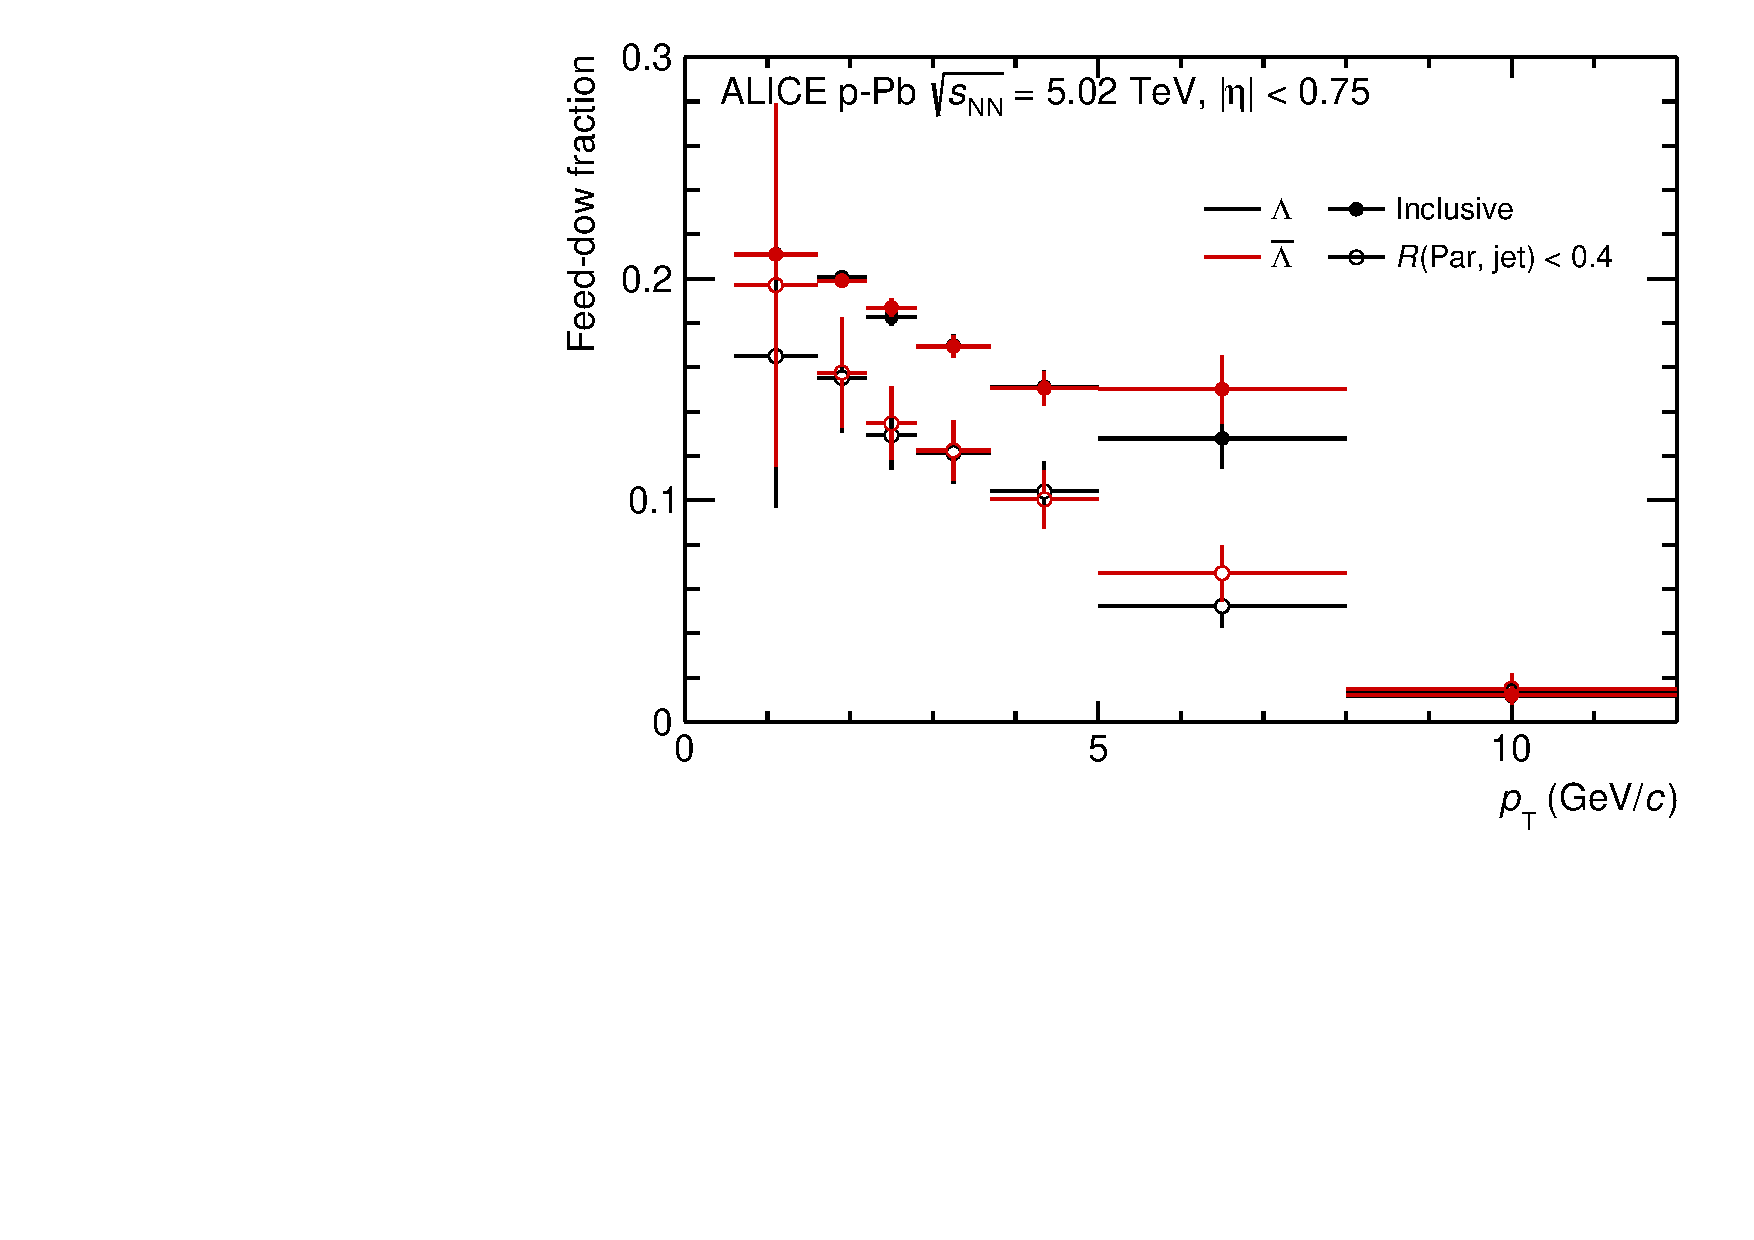
\includegraphics[width=.4\textwidth]{cf03_2}
%DIFDELCMD < 	%%%
\DIFdelendFL \DIFaddbeginFL 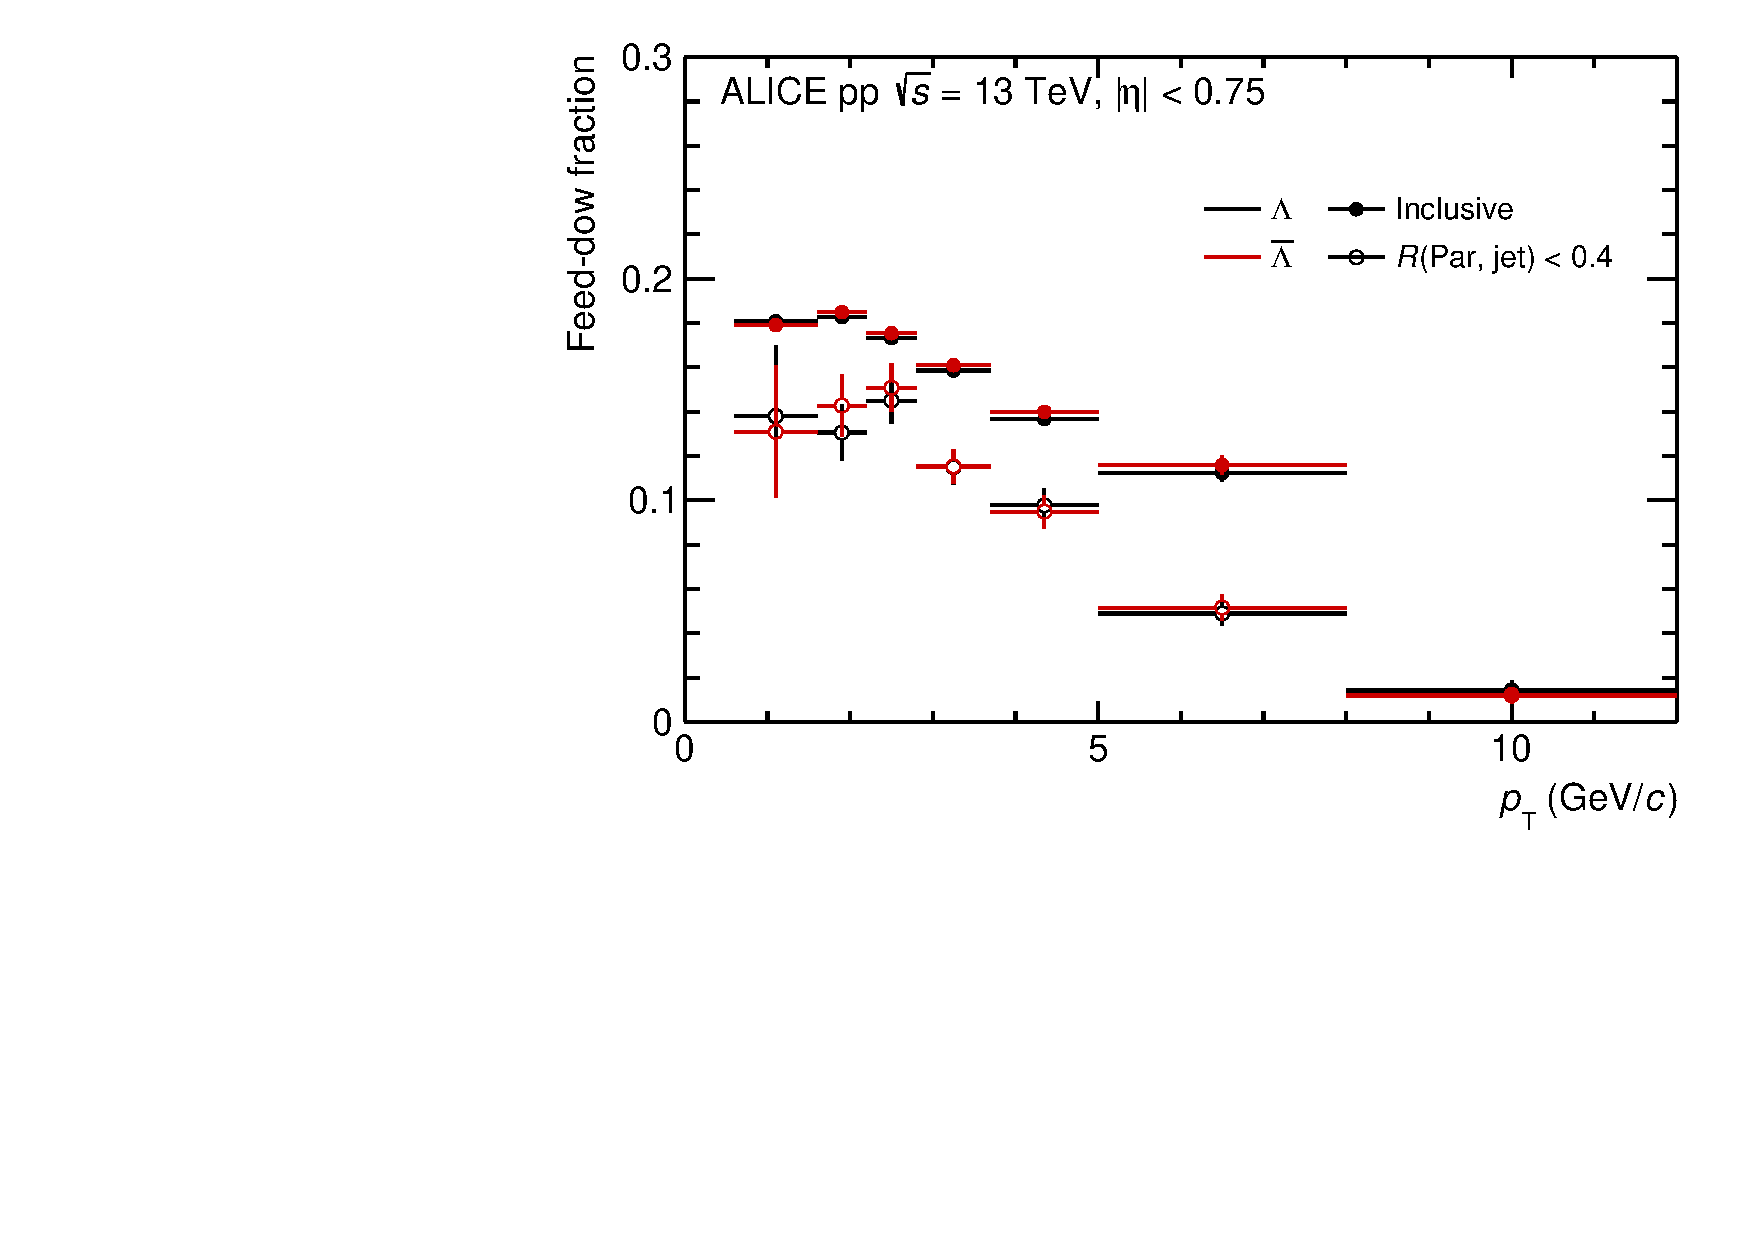
\includegraphics[width=.49\textwidth]{cf03_1}
		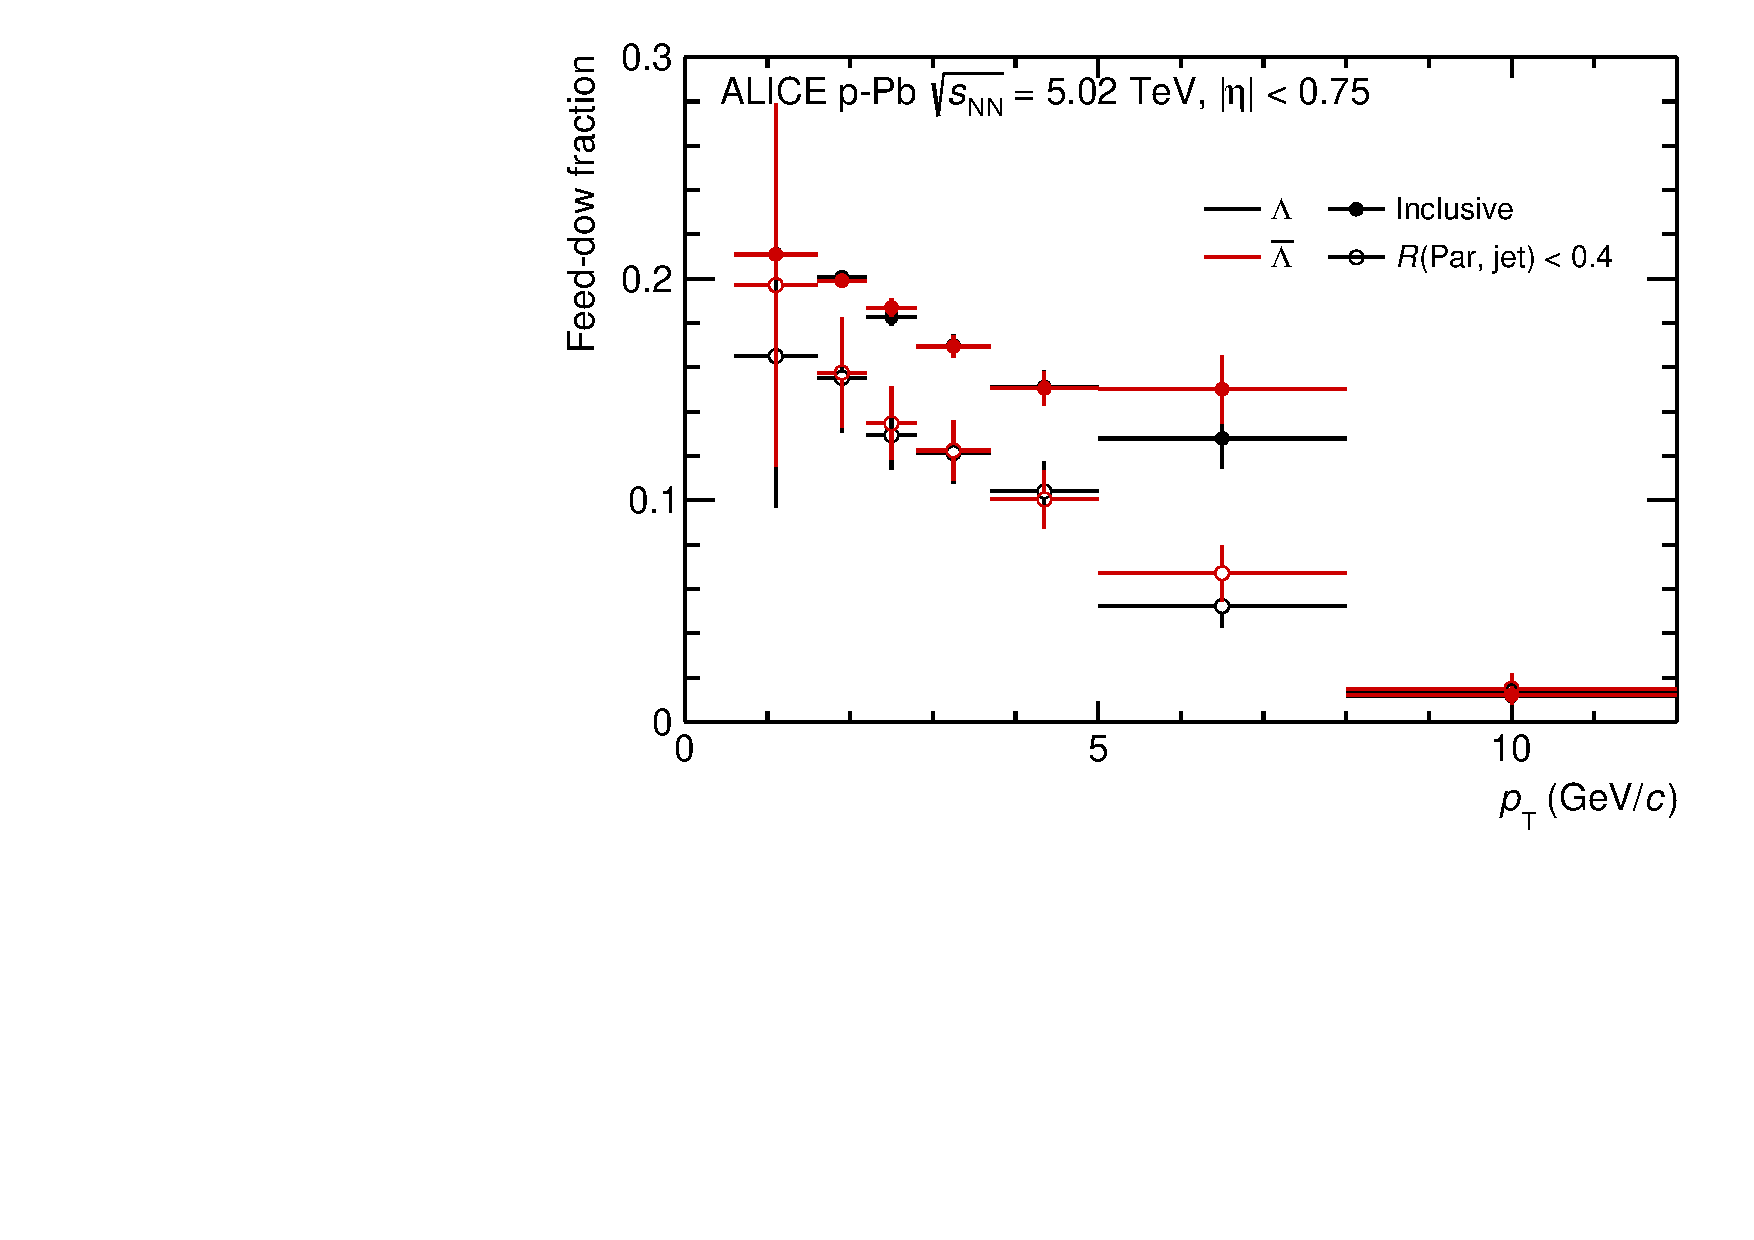
\includegraphics[width=.49\textwidth]{cf03_2}
	\DIFaddendFL \end{center}
	\caption{Fraction of $\lmb$ spectra removed due to feed-down subtraction of charged and neutral $\Xi$}
	\label{fig:FdFrac}
\end{figure}

\subsection{Systematic uncertainties}
\label{sec:SysUncer}
\DIFdelbegin \DIFdel{The total }\DIFdelend \DIFaddbegin \DIFadd{Total }\DIFaddend systematic uncertainty, for $\kzero$, $\lmb$, $\almb$, $\Xis$ and $\Oms$ \DIFdelbegin \DIFdel{reconstruction of each data point of the final results, due to the choice of selection criteria are }\DIFdelend \DIFaddbegin \DIFadd{yields have been }\DIFaddend estimated separately in each $\pT$ interval.
Individual settings are loosened and tightened, in order to measure changes in the signal loss correction.
The main sources of the systematic uncertainty in this measurements are \DIFaddbegin \DIFadd{related to the }\DIFaddend knowledge of detector materials, track selections, particle identification, proper lifetime, topological selection and signal extraction.
All these individual error contributions, which are listed in Tab.~\ref{tab:ppInclUncer}, \ref{tab:pPbInclUncer} are added in quadrature.
\begin{table}[!ht]
	\begin{center}
		\caption{Main sources and values of the relative systematic uncertainties (\%) of $\kzero$, $\lmb + \almb$, $\X + \Ix$ and $\Om + \Mo$ in \pp collisions at \thirteen.
			The \DIFdelbeginFL \DIFdelFL{value }\DIFdelendFL \DIFaddbeginFL \DIFaddFL{values }\DIFaddendFL are reported for low, intermediate and high $\pT$.}
		\label{tab:ppInclUncer}
		\begin{tabularx}{\textwidth}{@{} lCCCCCCCCCCCC @{}}
			\toprule
			\textbf{Uncertainty source} & \multicolumn{3}{c}{\textbf{$\kzero$}}
			& \multicolumn{3}{c}{\textbf{$\lmb + \almb$}}
			& \multicolumn{3}{c}{\textbf{$\X + \Ix$}}
			& \multicolumn{3}{c}{\textbf{$\Om + \Mo$}} \\
			\cmidrule(lr){2-4} \cmidrule(lr){5-7} \cmidrule(lr){8-10} \cmidrule(lr){11-13}
			$\pT$ (\GeVc)    & 0.6 & 2 &10  & 0.6 & 2 & 10  & 0.6 & 2 & 7   & 1& 2 & 5 \\
			\midrule
			Detector material & 4 & 4 & 4 & 4 & 4 & 4 & 4 & 4 & 4 & 4 & 4 & 4 \\
			Track selection &  1.5 & 1.2 & 0.4 & 0.6 & 1.4 & 1.3 & 2.8 & 0.1 & 0. & 0. & 1.5 & 0.2\\
			Particle identification& 0.1& 0.1& 0.1 & 0.3 & 0.2 & 1.1 & 1.9 & 1.7 & 2.4& 3.9& 8.7& 6.\\
			Proper lifetime& 0& 0.1& 0& 2.1& 0.4& 0& -& -& -& -& -& -\\
			Topological& 0.2& 1.4& 0& 3.9& 0.8& 3.9& 0.6& 0.9& 1.& 2.8& 5.4& 2.4\\
			Signal extraction& 0.8& 1.1& 1.1& 0.3& 0.5& 1.7& 3. & 1.& 0.5& 2.3& 4.6& 3 \\
			\midrule
			\textbf{Total uncertainty}& 4.4& 4.6& 4.2& 6.1& 4.4& 6.1& 6.1& 4.5& 4.8& 6.7& 12.& 8.2\\
			\bottomrule
		\end{tabularx}
	\end{center}
\end{table}

\begin{table}[!ht]
	\begin{center}
		\caption{Main sources and values of the relative systematic uncertainties (\%) of $\kzero$, $\lmb + \almb$, $\X + \Ix$ and $\Om + \Mo$ in \pPb collisions at \fivenn.
			The \DIFdelbeginFL \DIFdelFL{value }\DIFdelendFL \DIFaddbeginFL \DIFaddFL{values }\DIFaddendFL are reported for low, intermediate and high $\pT$ \DIFaddbeginFL \DIFaddFL{values}\DIFaddendFL .}
		\label{tab:pPbInclUncer}
		\begin{tabularx}{\textwidth}{@{} lCCCCCCCCCCCC @{}}
			\toprule
			\textbf{Uncertainty source} & \multicolumn{3}{c}{\textbf{\kzero}}
			& \multicolumn{3}{c}{\textbf{$\lmb + \almb$}}
			& \multicolumn{3}{c}{\textbf{$\X + \Ix$}}
			& \multicolumn{3}{c}{\textbf{$\Om + \Mo$}} \\
			\cmidrule(lr){2-4} \cmidrule(lr){5-7} \cmidrule(lr){8-10} \cmidrule(lr){11-13}
			$\pT$ (\GeVc) & 0.6 & 2 &10  & 0.6 & 2 & 10    & 0.6 & 2 & 7   & 1& 2 & 5 \\
			\midrule
			Detector material& 0.4 & 0.4 & 0.4 & 0.4 & 0.4 & 0.4 & 0.4 & 0.4 & 0.4 & 0.4 & 0.4 & 0.4 \\
			Track selection & 1.4& 1.7& 1.8& 0.2& 1.3& 1.4& 0& 0& 0& 1.3& 2.5& 0\\
			Particle identification& 0.1& 0.2& 0.2& 0.3& 0.2& 1& 3.1&  1.2& 0& 8.1& 13.7& 5.9 \\
			Proper lifetime & 0& 0& 0& 1.6& 0.3& 0& 0.6& 0.4& 0& 0& 3.3& 0\\
			Topological & 4.4& 0.6& 1.9& 3.9& 0.9& 2.7& 1.3& 0& 2.6& 1.2& 4.8& 3.7\\
			Signal extraction& 0.3& 2.6& 1.7& 0.6& 0.5& 2.6& 5.1& 0.9& 2.6& 0& 5.2& 0\\
			\midrule
			\textbf{Total uncertainty}& 6.1& 5.1& 5.1& 5.8& 4.3& 5.8& 7.4& 4.3& 5.4& 9.2& 16.4& 8\\
			\bottomrule
		\end{tabularx}
	\end{center}
\end{table}

\textbf{Material budget.} The effect of the incomplete knowledge of the detector's material budget is evaluated by comparing different Monte Carlo simulations in which the material budget was increased and decreased by $4.5\%$.
This value corresponds to the uncertainty on the determination of the material budget by measuring photon conversions\DIFaddbegin \DIFadd{~\mbox{%DIFAUXCMD
\cite{Abelev:2014ffa}}\hspace{0pt}%DIFAUXCMD
}\DIFaddend .
This particular systematic uncertainty is around \DIFdelbegin \DIFdel{$0.4\%$}\DIFdelend \DIFaddbegin \DIFadd{$4\%$~\mbox{%DIFAUXCMD
\cite{Acharya:2020uxl}}\hspace{0pt}%DIFAUXCMD
}\DIFaddend .

\textbf{Track selection.} To estimate the systematic \DIFaddbegin \DIFadd{uncertainty }\DIFaddend due to the track selection, the analysis has been redone with \DIFdelbegin \DIFdel{the }\DIFdelend \DIFaddbegin \DIFadd{an }\DIFaddend increased number of required clusters in the TPC \DIFaddbegin \DIFadd{from default 70 points to 80 points}\DIFaddend .

\textbf{Particle identification.} The TPC $\dEdx$ selection is used to reduce the combinatorial background in the (multi-)strange particle invariant mass distribution.
The number of \DIFaddbegin \DIFadd{Gaussian }\DIFaddend $\sigma$ in the identification of particles using the $\dEdx$ \DIFdelbegin \DIFdel{have been varied between }\DIFdelend \DIFaddbegin \DIFadd{has been varied from }\DIFaddend $4\sigma$ to $6\sigma$.

\textbf{Proper lifetime selection.} The proper lifetime \DIFdelbegin \DIFdel{defied }\DIFdelend \DIFaddbegin \DIFadd{is defined }\DIFaddend as $mLc/p$, \DIFdelbegin \DIFdel{which }\DIFdelend \DIFaddbegin \DIFadd{where }\DIFaddend $m$ is the mass of \DIFaddbegin \DIFadd{the }\DIFaddend particles, $L$ is the decay length, and $p$ is the particle's momentum.
The selection on the $mLc/p$ is varied \DIFdelbegin \DIFdel{from around }\DIFdelend \DIFaddbegin \DIFadd{within }\DIFaddend $12$ to $40$~cm for $\kzero$, $20$ to $40$ cm for $\lmb$ $(\almb)$\DIFdelbegin \DIFdel{and $2c\tau$ to $6c\tau$ }\DIFdelend \DIFaddbegin \DIFadd{, $10$ to $30$ cm }\DIFaddend for $\Xis$\DIFdelbegin \DIFdel{and }\DIFdelend \DIFaddbegin \DIFadd{, and $5$ to $15$ cm }\DIFaddend $\Oms$.

\textbf{Topological selection.} The values of the selection criteria \DIFdelbegin \DIFdel{on }\DIFdelend \DIFaddbegin \DIFadd{for }\DIFaddend the topological variables are varied \DIFaddbegin \DIFadd{within ranges leading to a maximum variation of $\pm 10\%$ in the raw singal yied }\DIFaddend around their nominal values.
The observed deviations for each component are summed in quadrature.

\textbf{Signal extraction.} In the same spirit, the signal extraction technique has been tested by varying the widths used to define the ``signal" and ``background'' regions, expressed in terms of the number of $\sigma$ as defined in Sec.~\ref{sec:ParRec}.
\DIFaddbegin \DIFadd{In particular the width of the peak region has been varied from the standard $6\sigma$ to $7\sigma$, $5\sigma$ and $4\sigma$ for }\Vzero \DIFadd{particles and  $3\sigma$ to $4\sigma~(3.5\sigma)$ and $2.5\sigma$ for $\Xi(\Omega)$.
}\DIFaddend 

The additional systematic uncertainty sources associated with particle yield in \DIFdelbegin \DIFdel{jet are originated }\DIFdelend \DIFaddbegin \DIFadd{the jet originate }\DIFaddend from the UE subtraction estimator and the jet $\pT$ threshold.
The systematic uncertainty due to the UE subtraction is estimated by varying the perpendicular cone radius from the chosen thresholds \DIFdelbegin \DIFdel{from }\DIFdelend \DIFaddbegin \DIFadd{of }\DIFaddend 0.4~(PC04) to 0.2~(PC02) and 0.6~(PC06).
From the \DIFdelbegin \DIFdel{deviation of }\DIFdelend \DIFaddbegin \DIFadd{deviations obtained for }\DIFaddend different PC cone size, the relative systematic uncertainty of the UE subtraction is \DIFdelbegin \DIFdel{obtained}\DIFdelend \DIFaddbegin \DIFadd{estimated}\DIFaddend .
To estimate the effect of jet $\pT$ \DIFdelbegin \DIFdel{thresholds }\DIFdelend \DIFaddbegin \DIFadd{threshold }\DIFaddend uncertainty, the analysis is repeated with the jet $\pT$ cut $10\pm 1$~\GeVc.
The systematic \DIFdelbegin \DIFdel{of the particle }\DIFdelend \DIFaddbegin \DIFadd{uncertainties of particles }\DIFaddend in jets are added to the list of uncertainties in quadrature.
The \DIFdelbegin \DIFdel{value }\DIFdelend \DIFaddbegin \DIFadd{values }\DIFaddend are shown in Table~\ref{tab:ppJEUncer}, \ref{tab:pPbJEUncer}.

\DIFaddbegin \DIFadd{The uncertainties of jet cone particle ratios ($\lmb/\kzero$, $\Xi/\kzero$, $\Omega/\kzero$, $\Xi/\lmb$, $\Omega/\lmb$ and $\Omega/\Xi$) also include three sources: the particle reconstruction, UE subtraction and the jet $\pT$ threshold.
The particle reconstruction uncertainty is propagated from the particle spectra.
Uncertainties related to UE subtraction and jet $\pT$ threshold are obtained by varying the same condition as particle spectra in both numerator and denominator of the corresponding ratios.
}

\DIFaddend \begin{table}[!ht]
	\begin{center}
		\caption{Main sources and values of the relative systematic uncertainties (\%) of \DIFaddbeginFL \DIFaddFL{particle $\pT$-differential density (}\DIFaddendFL $\kzero$, $\lmb + \almb$, $\X + \Ix$ and $\Om + \Mo$\DIFaddbeginFL \DIFaddFL{) and particle ratios ($\lmb/\kzero$, $\Xi/\kzero$, $\Omega/\kzero$, $\Xi/\lmb$, $\Omega/\lmb$ and $\Omega/\Xi$) }\DIFaddendFL in JE in \pp collisions at \thirteen.
			The \DIFdelbeginFL \DIFdelFL{value }\DIFdelendFL \DIFaddbeginFL \DIFaddFL{values }\DIFaddendFL are reported for low, intermediate and high $\pT$.}
		\label{tab:ppJEUncer}
		\begin{tabularx}{\textwidth}{@{} lCCCCCCCCCCCC @{}}
			\toprule
			\textbf{Uncertainty source} & \multicolumn{3}{c}{\textbf{\kzero}}
			& \multicolumn{3}{c}{\textbf{$\lmb + \almb$}}
			& \multicolumn{3}{c}{\textbf{$\X + \Ix$}}
			& \multicolumn{3}{c}{\textbf{$\Om + \Mo$}} \\
			\cmidrule(lr){2-4} \cmidrule(lr){5-7} \cmidrule(lr){8-10} \cmidrule(lr){11-13}
			$\pT$ (\GeVc) & 0.6 & 2 &10  & 0.6 & 2 & 10    & 0.6 & 2 & 7   & 1& 2 & 5 \\
			\midrule
			Particle reconstruction& 1.8& 0.25& 0.1& 5.3& 0.6& 0& 6.7& 0.9& 0.1& 6& 1.7& 0.3\\
			UE subtraction& 0.1& 0.1& 0.1& 0.1& 0.2& 0.1& 1.5& 0.2& 0.3& 3.6& 1.8& 0.5\\
			Jet $\pT$ threshold& 0.6& 3,1& 10.9& 0.6& 1.1& 9.9& 3.5& 2.4& 5& 0& 0& 0\\
			\midrule
			\textbf{Total uncertainty}& 1.8& 3.1& 10.9& 5.3& 1.2& 9.9& 7.7& 2.6& 5& 7.1& 2.5& 0.6 \\
			\bottomrule
		\end{tabularx}
	    \DIFdelbeginFL %DIFDELCMD < \end{center}
%DIFDELCMD < \end{table}
%DIFDELCMD < 

%DIFDELCMD < \begin{table}[!ht]
%DIFDELCMD < 	\begin{center}
%DIFDELCMD < 		%%%
%DIFDELCMD < \caption{%
{%DIFAUXCMD
\DIFdelFL{Main sources and values of the relative systematic uncertainties(\%) of $\kzero$, $\lmb + \almb$, $\X + \Ix$ and $\Om + \Mo$ in JE in }%DIFDELCMD < \pPb %%%
\DIFdelFL{collisions at }%DIFDELCMD < \fivenn%%%
\DIFdelFL{.
			The value are reported for low, intermediate and high $\pT$.}}
		%DIFAUXCMD
%DIFDELCMD < \label{tab:pPbJEUncer}
%DIFDELCMD < 		\begin{tabularx}{\textwidth}{@{} lCCCCCCCCCCCC @{}}
%DIFDELCMD < 			%%%
\DIFdelendFL \DIFaddbeginFL \begin{tabularx}{\textwidth}{@{} lCCCCCCCCC @{}}
	    	\DIFaddendFL \toprule
	    	\textbf{Uncertainty source} & \DIFdelbeginFL %DIFDELCMD < \multicolumn{3}{c}{\textbf{\kzero}}
%DIFDELCMD < 			& \multicolumn{3}{c}{\textbf{$\lmb + \almb$}}
%DIFDELCMD < 			%%%
\DIFdelendFL \DIFaddbeginFL \multicolumn{3}{c}{\textbf{$(\lmb + \almb)/(2\kzero)$}}
	    	\DIFaddendFL & \DIFdelbeginFL %DIFDELCMD < \multicolumn{3}{c}{\textbf{$\X + \Ix$}}
%DIFDELCMD < 			%%%
\DIFdelendFL \DIFaddbeginFL \multicolumn{3}{c}{\textbf{$(\X + \Ix)/(2\kzero)$}}
	    	\DIFaddendFL & \DIFdelbeginFL %DIFDELCMD < \multicolumn{3}{c}{\textbf{$\Om + \Mo$}} %%%
\DIFdelendFL \DIFaddbeginFL \multicolumn{3}{c}{\textbf{$(\Om + \Mo)/(2\kzero)$}} \DIFaddendFL \\
	    	\cmidrule(lr){2-4} \cmidrule(lr){5-7} \cmidrule(lr){8-10}
	    	\DIFdelbeginFL %DIFDELCMD < \cmidrule%%%
\DIFdelFL{(lr)}%DIFDELCMD < {%%%
\DIFdelFL{11-13}%DIFDELCMD < }
%DIFDELCMD < 			%%%
\DIFdelendFL $\pT$ (\GeVc) & 0.6 & 2 &10  & 0.6 & 2 & \DIFdelbeginFL \DIFdelFL{10    }%DIFDELCMD < & %%%
\DIFdelFL{0.6 }%DIFDELCMD < & %%%
\DIFdelFL{2 }%DIFDELCMD < & %%%
\DIFdelendFL 7 & 1 & 2 & 5 \\
	    	\midrule
	    	Particle reconstruction& \DIFdelbeginFL \DIFdelFL{5}%DIFDELCMD < & %%%
\DIFdelFL{0.8}%DIFDELCMD < & %%%
\DIFdelFL{0}%DIFDELCMD < & %%%
\DIFdelFL{13.2}\DIFdelendFL \DIFaddbeginFL \DIFaddFL{2.4}\DIFaddendFL & \DIFdelbeginFL \DIFdelFL{1.5}\DIFdelendFL \DIFaddbeginFL \DIFaddFL{2.8}\DIFaddendFL & \DIFdelbeginFL \DIFdelFL{0}\DIFdelendFL \DIFaddbeginFL \DIFaddFL{2.5}\DIFaddendFL & \DIFdelbeginFL \DIFdelFL{24.8}\DIFdelendFL \DIFaddbeginFL \DIFaddFL{3.4}\DIFaddendFL & 2.8& \DIFdelbeginFL \DIFdelFL{0.3}\DIFdelendFL \DIFaddbeginFL \DIFaddFL{2.8}\DIFaddendFL & \DIFdelbeginFL \DIFdelFL{8.7}\DIFdelendFL \DIFaddbeginFL \DIFaddFL{6.7}\DIFaddendFL & \DIFdelbeginFL \DIFdelFL{3.7}\DIFdelendFL \DIFaddbeginFL \DIFaddFL{11.4}\DIFaddendFL & \DIFdelbeginFL \DIFdelFL{0.9}\DIFdelendFL \DIFaddbeginFL \DIFaddFL{7.3}\DIFaddendFL \\
	    	UE subtraction& \DIFdelbeginFL \DIFdelFL{0.3}%DIFDELCMD < & %%%
\DIFdelFL{0.1}%DIFDELCMD < & %%%
\DIFdelFL{0.1}%DIFDELCMD < & %%%
\DIFdelFL{0}\DIFdelendFL \DIFaddbeginFL \DIFaddFL{0.8}\DIFaddendFL & \DIFdelbeginFL \DIFdelFL{0.1}\DIFdelendFL \DIFaddbeginFL \DIFaddFL{0.2}\DIFaddendFL & \DIFdelbeginFL \DIFdelFL{11.2}\DIFdelendFL \DIFaddbeginFL \DIFaddFL{0.4}\DIFaddendFL & \DIFdelbeginFL \DIFdelFL{14.1}\DIFdelendFL \DIFaddbeginFL \DIFaddFL{3.5}\DIFaddendFL & \DIFdelbeginFL \DIFdelFL{0.8}\DIFdelendFL \DIFaddbeginFL \DIFaddFL{0.2}\DIFaddendFL & \DIFdelbeginFL \DIFdelFL{0.7}\DIFdelendFL \DIFaddbeginFL \DIFaddFL{0.1}\DIFaddendFL & \DIFdelbeginFL \DIFdelFL{0}\DIFdelendFL \DIFaddbeginFL \DIFaddFL{10}\DIFaddendFL & \DIFdelbeginFL \DIFdelFL{0}\DIFdelendFL \DIFaddbeginFL \DIFaddFL{4}\DIFaddendFL & \DIFdelbeginFL \DIFdelFL{1.2}\DIFdelendFL \DIFaddbeginFL \DIFaddFL{2.2}\DIFaddendFL \\
	    	Jet $\pT$ threshold& \DIFdelbeginFL \DIFdelFL{0.3}%DIFDELCMD < & %%%
\DIFdelFL{3.5}%DIFDELCMD < & %%%
\DIFdelFL{11}%DIFDELCMD < & %%%
\DIFdelFL{3.2}\DIFdelendFL \DIFaddbeginFL \DIFaddFL{0.4}\DIFaddendFL & \DIFdelbeginFL \DIFdelFL{1.8}\DIFdelendFL \DIFaddbeginFL \DIFaddFL{2.3}\DIFaddendFL & \DIFdelbeginFL \DIFdelFL{0.1}\DIFdelendFL \DIFaddbeginFL \DIFaddFL{1}\DIFaddendFL & \DIFdelbeginFL \DIFdelFL{24.9}\DIFdelendFL \DIFaddbeginFL \DIFaddFL{1.7}\DIFaddendFL & \DIFdelbeginFL \DIFdelFL{3}\DIFdelendFL \DIFaddbeginFL \DIFaddFL{1.6}\DIFaddendFL & \DIFdelbeginFL \DIFdelFL{4.1}\DIFdelendFL \DIFaddbeginFL \DIFaddFL{3.6}\DIFaddendFL & \DIFdelbeginFL \DIFdelFL{3.1}\DIFdelendFL \DIFaddbeginFL \DIFaddFL{1.}\DIFaddendFL & \DIFdelbeginFL \DIFdelFL{10.7}\DIFdelendFL \DIFaddbeginFL \DIFaddFL{3.3}\DIFaddendFL & \DIFdelbeginFL \DIFdelFL{7.6}\DIFdelendFL \DIFaddbeginFL \DIFaddFL{6.4}\DIFaddendFL \\
	    	\midrule
	    	\textbf{Total uncertainty}& \DIFdelbeginFL \DIFdelFL{5}%DIFDELCMD < & %%%
\DIFdelFL{3.6}%DIFDELCMD < & %%%
\DIFdelFL{11}%DIFDELCMD < & %%%
\DIFdelFL{13.5}\DIFdelendFL \DIFaddbeginFL \DIFaddFL{2.6}\DIFaddendFL & \DIFdelbeginFL \DIFdelFL{2.3}\DIFdelendFL \DIFaddbeginFL \DIFaddFL{3.7}\DIFaddendFL & \DIFdelbeginFL \DIFdelFL{11.2}\DIFdelendFL \DIFaddbeginFL \DIFaddFL{2.7}\DIFaddendFL & \DIFdelbeginFL \DIFdelFL{37.9}\DIFdelendFL \DIFaddbeginFL \DIFaddFL{5.2}\DIFaddendFL & \DIFdelbeginFL \DIFdelFL{4.2}\DIFdelendFL \DIFaddbeginFL \DIFaddFL{3.3}\DIFaddendFL & \DIFdelbeginFL \DIFdelFL{4.1}\DIFdelendFL \DIFaddbeginFL \DIFaddFL{4.5}\DIFaddendFL & \DIFdelbeginFL \DIFdelFL{9.3}\DIFdelendFL \DIFaddbeginFL \DIFaddFL{12.4}\DIFaddendFL & \DIFdelbeginFL \DIFdelFL{11.3}\DIFdelendFL \DIFaddbeginFL \DIFaddFL{12.5}\DIFaddendFL & \DIFdelbeginFL \DIFdelFL{7.7 }\DIFdelendFL \DIFaddbeginFL \DIFaddFL{10}\DIFaddendFL \\
	    	\bottomrule
	    \end{tabularx}
		\DIFdelbeginFL %DIFDELCMD < \end{center}
%DIFDELCMD < \end{table}
%DIFDELCMD < 

%DIFDELCMD < %%%
\DIFdel{The uncertainty of jet cone particle ratios ($\lmb/\kzero$, $\Xi/\kzero$, $\Omega/\kzero$, $\Xi/\lmb$, $\Omega/\lmb$ and $\Omega/\Xi$) also consider three sources: the particle reconstruction, UE subtraction and the jet $\pT$ threshold.
The particle reconstruction uncertainty is propagated from the spectra.
Uncertainties related to UE subtraction and jet $\pT$ threshold are obtained by varying the condition in both numerator and denominator of the corresponding ratios.
}%DIFDELCMD < 

%DIFDELCMD < \begin{table}[!ht]
%DIFDELCMD < 	\begin{center}
%DIFDELCMD < 		%%%
%DIFDELCMD < \caption{%
{%DIFAUXCMD
\DIFdelFL{Main sources and values of the relative systematic uncertainties(\%) of baryon-to-meson ratios ($\lmb/\kzero$, $\Xi/\kzero$, $\Omega/\kzero$) in JE in }%DIFDELCMD < \pp %%%
\DIFdelFL{collisions at }%DIFDELCMD < \thirteen%%%
\DIFdelFL{.
			The value are reported for low, intermediate and high $\pT$.}}
		%DIFAUXCMD
%DIFDELCMD < \label{tab:ppBMRatioUncer}
%DIFDELCMD < 		%%%
\DIFdelendFL \begin{tabularx}{\textwidth}{@{} lCCCCCCCCC @{}}
			\toprule
			\textbf{Uncertainty source} & \DIFdelbeginFL %DIFDELCMD < \multicolumn{3}{c}{\textbf{$(\lmb + \almb)/(2\kzero)$}}
%DIFDELCMD < 			%%%
\DIFdelendFL \DIFaddbeginFL \multicolumn{3}{c}{\textbf{$(\X + \Ix)/(\lmb + \almb)$}}
			\DIFaddendFL & \DIFdelbeginFL %DIFDELCMD < \multicolumn{3}{c}{\textbf{$(\X + \Ix)/(2\kzero)$}}
%DIFDELCMD < 			%%%
\DIFdelendFL \DIFaddbeginFL \multicolumn{3}{c}{\textbf{$(\Om + \Mo)/(\lmb + \almb)$}}
			\DIFaddendFL & \DIFdelbeginFL %DIFDELCMD < \multicolumn{3}{c}{\textbf{$(\Om + \Mo)/(2\kzero)$}} %%%
\DIFdelendFL \DIFaddbeginFL \multicolumn{3}{c}{\textbf{$(\Om + \Mo)/(\X + \Ix)$}} \DIFaddendFL \\
			\cmidrule(lr){2-4} \cmidrule(lr){5-7} \cmidrule(lr){8-10}
			$\pT$ (\GeVc) & 0.6 & 2 &\DIFdelbeginFL \DIFdelFL{10  }\DIFdelendFL \DIFaddbeginFL \DIFaddFL{7  }\DIFaddendFL & \DIFdelbeginFL \DIFdelFL{0.6 }\DIFdelendFL \DIFaddbeginFL \DIFaddFL{1 }\DIFaddendFL & 2 & \DIFdelbeginFL \DIFdelFL{7 }\DIFdelendFL \DIFaddbeginFL \DIFaddFL{5 }\DIFaddendFL & 1 & 2 & 5 \\
			\midrule
			Particle reconstruction& \DIFdelbeginFL \DIFdelFL{2.4}\DIFdelendFL \DIFaddbeginFL \DIFaddFL{3.4}\DIFaddendFL & \DIFdelbeginFL \DIFdelFL{2.8}\DIFdelendFL \DIFaddbeginFL \DIFaddFL{3}\DIFaddendFL & \DIFdelbeginFL \DIFdelFL{2.5}\DIFdelendFL \DIFaddbeginFL \DIFaddFL{3.2}\DIFaddendFL & \DIFdelbeginFL \DIFdelFL{3.4}\DIFdelendFL \DIFaddbeginFL \DIFaddFL{6.7}\DIFaddendFL & \DIFdelbeginFL \DIFdelFL{2.8}\DIFdelendFL \DIFaddbeginFL \DIFaddFL{11.5}\DIFaddendFL & \DIFdelbeginFL \DIFdelFL{2.8}\DIFdelendFL \DIFaddbeginFL \DIFaddFL{7.5}\DIFaddendFL & \DIFdelbeginFL \DIFdelFL{6.7}\DIFdelendFL \DIFaddbeginFL \DIFaddFL{6.8}\DIFaddendFL & \DIFdelbeginFL \DIFdelFL{11.4}\DIFdelendFL \DIFaddbeginFL \DIFaddFL{11.5}\DIFaddendFL & \DIFdelbeginFL \DIFdelFL{7.3}\DIFdelendFL \DIFaddbeginFL \DIFaddFL{7.4}\DIFaddendFL \\
			UE subtraction& \DIFdelbeginFL \DIFdelFL{0.8}%DIFDELCMD < & %%%
\DIFdelFL{0.2}\DIFdelendFL \DIFaddbeginFL \DIFaddFL{4.4}\DIFaddendFL & 0.4& \DIFdelbeginFL \DIFdelFL{3.5}%DIFDELCMD < & %%%
\DIFdelendFL 0.2& \DIFdelbeginFL \DIFdelFL{0.1}\DIFdelendFL \DIFaddbeginFL \DIFaddFL{12.4}\DIFaddendFL & \DIFdelbeginFL \DIFdelFL{10}\DIFdelendFL \DIFaddbeginFL \DIFaddFL{4.2}\DIFaddendFL & \DIFdelbeginFL \DIFdelFL{4}\DIFdelendFL \DIFaddbeginFL \DIFaddFL{2.3}\DIFaddendFL & \DIFdelbeginFL \DIFdelFL{2.2}\DIFdelendFL \DIFaddbeginFL \DIFaddFL{7.8}& \DIFaddFL{3.8}& \DIFaddFL{2.7}\DIFaddendFL \\
		    Jet $\pT$ threshold& \DIFdelbeginFL \DIFdelFL{0.4}\DIFdelendFL \DIFaddbeginFL \DIFaddFL{0.7}\DIFaddendFL & \DIFdelbeginFL \DIFdelFL{2.3}\DIFdelendFL \DIFaddbeginFL \DIFaddFL{0.5}\DIFaddendFL & \DIFdelbeginFL \DIFdelFL{1}\DIFdelendFL \DIFaddbeginFL \DIFaddFL{1.9}\DIFaddendFL & \DIFdelbeginFL \DIFdelFL{1.7}\DIFdelendFL \DIFaddbeginFL \DIFaddFL{0.2}\DIFaddendFL & \DIFdelbeginFL \DIFdelFL{1.6}\DIFdelendFL \DIFaddbeginFL \DIFaddFL{0.9}\DIFaddendFL & \DIFdelbeginFL \DIFdelFL{3.6}\DIFdelendFL \DIFaddbeginFL \DIFaddFL{3.5}\DIFaddendFL & \DIFdelbeginFL \DIFdelFL{1.}\DIFdelendFL \DIFaddbeginFL \DIFaddFL{0.4}\DIFaddendFL & \DIFdelbeginFL \DIFdelFL{3.3}\DIFdelendFL \DIFaddbeginFL \DIFaddFL{1.3}\DIFaddendFL & \DIFdelbeginFL \DIFdelFL{6.4}\DIFdelendFL \DIFaddbeginFL \DIFaddFL{3}\DIFaddendFL \\
		    \midrule
		    \textbf{Total uncertainty}& \DIFdelbeginFL \DIFdelFL{2.6}\DIFdelendFL \DIFaddbeginFL \DIFaddFL{5.6}\DIFaddendFL & \DIFdelbeginFL \DIFdelFL{3.7}\DIFdelendFL \DIFaddbeginFL \DIFaddFL{3}\DIFaddendFL & \DIFdelbeginFL \DIFdelFL{2.7}\DIFdelendFL \DIFaddbeginFL \DIFaddFL{3.7}\DIFaddendFL & \DIFdelbeginFL \DIFdelFL{5.2}\DIFdelendFL \DIFaddbeginFL \DIFaddFL{14.1}\DIFaddendFL & \DIFdelbeginFL \DIFdelFL{3.3}\DIFdelendFL \DIFaddbeginFL \DIFaddFL{12.2}\DIFaddendFL & \DIFdelbeginFL \DIFdelFL{4.5}\DIFdelendFL \DIFaddbeginFL \DIFaddFL{8.6}\DIFaddendFL & \DIFdelbeginFL \DIFdelFL{12.4}\DIFdelendFL \DIFaddbeginFL \DIFaddFL{10.3}\DIFaddendFL & \DIFdelbeginFL \DIFdelFL{12.5}\DIFdelendFL \DIFaddbeginFL \DIFaddFL{12.1}\DIFaddendFL & \DIFdelbeginFL \DIFdelFL{10}\DIFdelendFL \DIFaddbeginFL \DIFaddFL{8.5}\DIFaddendFL \\
	 	    \bottomrule
	  \end{tabularx}
	\end{center}
\end{table}

\begin{table}[!ht]
	\begin{center}
		\caption{Main sources and values of the relative systematic uncertainties (\%) of \DIFdelbeginFL \DIFdelFL{baryon-to-baryon }\DIFdelendFL \DIFaddbeginFL \DIFaddFL{particle $\pT$-differential density ($\kzero$, $\lmb + \almb$, $\X + \Ix$ and $\Om + \Mo$) and particle }\DIFaddendFL ratios (\DIFaddbeginFL \DIFaddFL{$\lmb/\kzero$, $\Xi/\kzero$, $\Omega/\kzero$, }\DIFaddendFL $\Xi/\lmb$, $\Omega/\lmb$ \DIFdelbeginFL \DIFdelFL{, }\DIFdelendFL \DIFaddbeginFL \DIFaddFL{and }\DIFaddendFL $\Omega/\Xi$) in JE in \DIFdelbeginFL %DIFDELCMD < \pp %%%
\DIFdelendFL \DIFaddbeginFL \pPb \DIFaddendFL collisions at \DIFdelbeginFL %DIFDELCMD < \thirteen%%%
\DIFdelendFL \DIFaddbeginFL \fivenn\DIFaddendFL .
			The \DIFdelbeginFL \DIFdelFL{value }\DIFdelendFL \DIFaddbeginFL \DIFaddFL{values }\DIFaddendFL are reported for low, intermediate and high $\pT$.}
		\DIFdelbeginFL %DIFDELCMD < \label{tab:ppBBRatioUncer}
%DIFDELCMD < 		\begin{tabularx}{\textwidth}{@{} lCCCCCCCCC @{}}
%DIFDELCMD < 			%%%
\DIFdelendFL \DIFaddbeginFL \label{tab:pPbJEUncer}
		\begin{tabularx}{\textwidth}{@{} lCCCCCCCCCCCC @{}}
			\DIFaddendFL \toprule
			\textbf{Uncertainty source} & \DIFdelbeginFL %DIFDELCMD < \multicolumn{3}{c}{\textbf{$(\X + \Ix)/(\lmb + \almb)$}}
%DIFDELCMD < 			%%%
\DIFdelendFL \DIFaddbeginFL \multicolumn{3}{c}{\textbf{\kzero}}
			\DIFaddendFL & \DIFdelbeginFL %DIFDELCMD < \multicolumn{3}{c}{\textbf{$(\Om + \Mo)/(\lmb + \almb)$}}
%DIFDELCMD < 			%%%
\DIFdelendFL \DIFaddbeginFL \multicolumn{3}{c}{\textbf{$\lmb + \almb$}}
			\DIFaddendFL & \DIFdelbeginFL %DIFDELCMD < \multicolumn{3}{c}{\textbf{$(\Om + \Mo)/(\X + \Ix)$}} %%%
\DIFdelendFL \DIFaddbeginFL \multicolumn{3}{c}{\textbf{$\X + \Ix$}}
			& \multicolumn{3}{c}{\textbf{$\Om + \Mo$}} \DIFaddendFL \\
			\cmidrule(lr){2-4} \cmidrule(lr){5-7} \cmidrule(lr){8-10} \DIFaddbeginFL \cmidrule\DIFaddFL{(lr)}{\DIFaddFL{11-13}}
			\DIFaddendFL $\pT$ (\GeVc) & 0.6 & 2 &\DIFdelbeginFL \DIFdelFL{7  }\DIFdelendFL \DIFaddbeginFL \DIFaddFL{10  }\DIFaddendFL & \DIFdelbeginFL \DIFdelFL{1 }\DIFdelendFL \DIFaddbeginFL \DIFaddFL{0.6 }\DIFaddendFL & 2 & \DIFdelbeginFL \DIFdelFL{5 }\DIFdelendFL \DIFaddbeginFL \DIFaddFL{10    }& \DIFaddFL{0.6 }& \DIFaddFL{2 }& \DIFaddFL{7   }\DIFaddendFL & 1& 2 & 5 \\
			\midrule
			Particle reconstruction& \DIFdelbeginFL \DIFdelFL{3.4}\DIFdelendFL \DIFaddbeginFL \DIFaddFL{5}\DIFaddendFL & \DIFdelbeginFL \DIFdelFL{3}\DIFdelendFL \DIFaddbeginFL \DIFaddFL{0.8}\DIFaddendFL & \DIFdelbeginFL \DIFdelFL{3.2}\DIFdelendFL \DIFaddbeginFL \DIFaddFL{0}\DIFaddendFL & \DIFdelbeginFL \DIFdelFL{6.7}\DIFdelendFL \DIFaddbeginFL \DIFaddFL{13.2}\DIFaddendFL & \DIFdelbeginFL \DIFdelFL{11.5}\DIFdelendFL \DIFaddbeginFL \DIFaddFL{1.5}\DIFaddendFL & \DIFdelbeginFL \DIFdelFL{7.5}\DIFdelendFL \DIFaddbeginFL \DIFaddFL{0}\DIFaddendFL & \DIFdelbeginFL \DIFdelFL{6.8}\DIFdelendFL \DIFaddbeginFL \DIFaddFL{24.8}\DIFaddendFL & \DIFdelbeginFL \DIFdelFL{11.5}\DIFdelendFL \DIFaddbeginFL \DIFaddFL{2.8}\DIFaddendFL & \DIFdelbeginFL \DIFdelFL{7.4}\DIFdelendFL \DIFaddbeginFL \DIFaddFL{0.3}& \DIFaddFL{8.7}& \DIFaddFL{3.7}& \DIFaddFL{0.9}\DIFaddendFL \\
			UE subtraction& \DIFdelbeginFL \DIFdelFL{4.4}\DIFdelendFL \DIFaddbeginFL \DIFaddFL{0.3}\DIFaddendFL & \DIFdelbeginFL \DIFdelFL{0.4}\DIFdelendFL \DIFaddbeginFL \DIFaddFL{0.1}\DIFaddendFL & \DIFdelbeginFL \DIFdelFL{0.2}\DIFdelendFL \DIFaddbeginFL \DIFaddFL{0.1}\DIFaddendFL & \DIFdelbeginFL \DIFdelFL{12.4}\DIFdelendFL \DIFaddbeginFL \DIFaddFL{0}\DIFaddendFL & \DIFdelbeginFL \DIFdelFL{4.2}\DIFdelendFL \DIFaddbeginFL \DIFaddFL{0.1}\DIFaddendFL & \DIFdelbeginFL \DIFdelFL{2.3}\DIFdelendFL \DIFaddbeginFL \DIFaddFL{11.2}\DIFaddendFL & \DIFdelbeginFL \DIFdelFL{7.8}\DIFdelendFL \DIFaddbeginFL \DIFaddFL{14.1}\DIFaddendFL & \DIFdelbeginFL \DIFdelFL{3.8}\DIFdelendFL \DIFaddbeginFL \DIFaddFL{0.8}\DIFaddendFL & \DIFdelbeginFL \DIFdelFL{2.7}\DIFdelendFL \DIFaddbeginFL \DIFaddFL{0.7}& \DIFaddFL{0}& \DIFaddFL{0}& \DIFaddFL{1.2}\DIFaddendFL \\
			Jet $\pT$ threshold& \DIFdelbeginFL \DIFdelFL{0.7}%DIFDELCMD < & %%%
\DIFdelFL{0.5}\DIFdelendFL \DIFaddbeginFL \DIFaddFL{0.3}\DIFaddendFL & \DIFdelbeginFL \DIFdelFL{1.9}\DIFdelendFL \DIFaddbeginFL \DIFaddFL{3.5}\DIFaddendFL & \DIFdelbeginFL \DIFdelFL{0.2}\DIFdelendFL \DIFaddbeginFL \DIFaddFL{11}\DIFaddendFL & \DIFdelbeginFL \DIFdelFL{0.9}\DIFdelendFL \DIFaddbeginFL \DIFaddFL{3.2}\DIFaddendFL & \DIFdelbeginFL \DIFdelFL{3.5}\DIFdelendFL \DIFaddbeginFL \DIFaddFL{1.8}\DIFaddendFL & \DIFdelbeginFL \DIFdelFL{0.4}\DIFdelendFL \DIFaddbeginFL \DIFaddFL{0.1}\DIFaddendFL & \DIFdelbeginFL \DIFdelFL{1.3}\DIFdelendFL \DIFaddbeginFL \DIFaddFL{24.9}\DIFaddendFL &  3\DIFaddbeginFL & \DIFaddFL{4.1}& \DIFaddFL{3.1}& \DIFaddFL{10.7}& \DIFaddFL{7.6}\DIFaddendFL \\
			\midrule
			\textbf{Total uncertainty}& \DIFdelbeginFL \DIFdelFL{5.6}\DIFdelendFL \DIFaddbeginFL \DIFaddFL{5}\DIFaddendFL & \DIFdelbeginFL \DIFdelFL{3}\DIFdelendFL \DIFaddbeginFL \DIFaddFL{3.6}\DIFaddendFL & \DIFdelbeginFL \DIFdelFL{3.7}\DIFdelendFL \DIFaddbeginFL \DIFaddFL{11}\DIFaddendFL & \DIFdelbeginFL \DIFdelFL{14.1}\DIFdelendFL \DIFaddbeginFL \DIFaddFL{13.5}\DIFaddendFL & \DIFdelbeginFL \DIFdelFL{12.2}\DIFdelendFL \DIFaddbeginFL \DIFaddFL{2.3}\DIFaddendFL & \DIFdelbeginFL \DIFdelFL{8.6}\DIFdelendFL \DIFaddbeginFL \DIFaddFL{11.2}\DIFaddendFL & \DIFdelbeginFL \DIFdelFL{10.3}\DIFdelendFL \DIFaddbeginFL \DIFaddFL{37.9}\DIFaddendFL & \DIFdelbeginFL \DIFdelFL{12.1}\DIFdelendFL \DIFaddbeginFL \DIFaddFL{4.2}\DIFaddendFL & \DIFdelbeginFL \DIFdelFL{8.5}\DIFdelendFL \DIFaddbeginFL \DIFaddFL{4.1}& \DIFaddFL{9.3}& \DIFaddFL{11.3}& \DIFaddFL{7.7 }\DIFaddendFL \\
			\bottomrule
		\end{tabularx}
		\DIFdelbeginFL %DIFDELCMD < \end{center}
%DIFDELCMD < \end{table}
%DIFDELCMD < 

%DIFDELCMD < \begin{table}[!ht]
%DIFDELCMD < 	\begin{center}
%DIFDELCMD < 		%%%
%DIFDELCMD < \caption{%
{%DIFAUXCMD
\DIFdelFL{Main sources and values of the relative systematic uncertainties(\%) of baryon-to-meson ratios ($\lmb/\kzero$, $\Xi/\kzero$, $\Omega/\kzero$) in JE in }%DIFDELCMD < \pPb %%%
\DIFdelFL{collisions at }%DIFDELCMD < \fivenn%%%
\DIFdelFL{.
			The value are reported for low, intermediate and high $\pT$.}}
		%DIFAUXCMD
%DIFDELCMD < \label{tab:pPbBMRatioUncer}
%DIFDELCMD < 		%%%
\DIFdelendFL \begin{tabularx}{\textwidth}{@{} lCCCCCCCCC @{}}
		    \toprule
		    \textbf{Uncertainty source} & \multicolumn{3}{c}{\textbf{$(\lmb + \almb)/(2\kzero)$}}
		    & \multicolumn{3}{c}{\textbf{$(\X + \Ix)/(2\kzero)$}}
		    & \multicolumn{3}{c}{\textbf{$(\Om + \Mo)/(2\kzero)$}} \\
	  	    \cmidrule(lr){2-4} \cmidrule(lr){5-7} \cmidrule(lr){8-10}
		    $\pT$ (\GeVc) & 0.6 & 2 &10  & 0.6 & 2 & 7 & 1 & 2 & 5 \\
		    \midrule
		    Particle reconstruction& 3.2& 3.4& 3.3& 4.7& 3.2& 4& 9.8& 1.5& 7.4\\
	 	    UE subtraction& 0.8& 0.1& 0.1& 9.1& 1.8& 1& 4.1& 0& 0.3\\
		    Jet $\pT$ threshold& 1.4& 2.6& 0.1& 8.6& 2.4& 6& 0.5& 1.5& 0.3\\
		    \midrule
		    \textbf{Total uncertainty}& 3.6& 4.3& 3.3& 13.4& 4.4& 7.2& 10.6& 15.1& 7.4\\
		    \bottomrule
	        \end{tabularx}
	        \DIFdelbeginFL %DIFDELCMD < \end{center}
%DIFDELCMD < \end{table}
%DIFDELCMD < \begin{table}[!ht]
%DIFDELCMD < 	\begin{center}
%DIFDELCMD < 		%%%
%DIFDELCMD < \caption{%
{%DIFAUXCMD
\DIFdelFL{Main sources and values of the relative systematic uncertainties(\%) of baryon-to-baryon ratios ($\Xi/\lmb$, $\Omega/\lmb$, $\Omega/\Xi$) in JE in }%DIFDELCMD < \pPb %%%
\DIFdelFL{collisions at }%DIFDELCMD < \fivenn%%%
\DIFdelFL{.
			The value are reported for low, intermediate and high $\pT$.}}
		%DIFAUXCMD
%DIFDELCMD < \label{tab:pPbBBRatioUncer}
%DIFDELCMD < 		%%%
\DIFdelendFL \begin{tabularx}{\textwidth}{@{} lCCCCCCCCC @{}}
		    \toprule
		    \textbf{Uncertainty source} & \multicolumn{3}{c}{\textbf{$(\X + \Ix)/(\lmb + \almb)$}}
		    & \multicolumn{3}{c}{\textbf{$(\Om + \Mo)/(\lmb + \almb)$}}
		    & \multicolumn{3}{c}{\textbf{$(\Om + \Mo)/(\X + \Ix)$}} \\
		    \cmidrule(lr){2-4} \cmidrule(lr){5-7} \cmidrule(lr){8-10}
		    $\pT$ (\GeVc) & 0.6 & 2 &10  & 0.6 & 2 & 7 & 1 & 2 & 5 \\
		    \midrule
		    Particle reconstruction& 4.1& 2.8& 3.7& 9.6& 15& 7.5& 10& 14.9& 8.6\\
		    UE subtraction& 9.9& 1.9& 0.8& 3.6& 0.1& 0.3& 11& 1.8& 0.1\\
		    Jet $\pT$ threshold& 2.7& 0.6& 2.6& 0.4& 5& 3& 0.4& 3.8& 1.7\\
		    \midrule
		    \textbf{Total uncertainty}& 11.1& 3.4& 4.6& 10.3& 15.8& 8.1& 14.9& 15.5& 8.7\\
		    \bottomrule
	\end{tabularx}
	\end{center}
\end{table}

\DIFaddbegin \clearpage

\DIFaddend \section{Results and discussion}%
\label{sec:Results}

\subsection{Particles $\pT$-differential density}
\label{subsec:ParPtDensity}

For the strange hadrons discussed in this paper, the ratios of yields for particles and anti-particles are around one within the uncertainties, as expected at these collision energies in the mid-rapidity region\DIFaddbegin \DIFadd{~\mbox{%DIFAUXCMD
\cite{Acharya:2020uxl, ALICE:2015mpp}}\hspace{0pt}%DIFAUXCMD
}\DIFaddend .
Therefore, all the $\pT$-differential \DIFdelbegin \DIFdel{density is shown in the following }\DIFdelend \DIFaddbegin \DIFadd{densities }\DIFaddend are reported after summing \DIFdelbegin \DIFdel{particles }\DIFdelend \DIFaddbegin \DIFadd{over particle }\DIFaddend and anti-particles.
The different selections shown \DIFdelbegin \DIFdel{in the following }\DIFdelend \DIFaddbegin \DIFadd{below }\DIFaddend have been introduced in \DIFdelbegin \DIFdel{section}\DIFdelend \DIFaddbegin \DIFadd{Sec.}\DIFaddend ~\ref{sec:ParJetMatch}, \DIFdelbegin \DIFdel{inwhich also introduced the normalization method }\DIFdelend \DIFaddbegin \DIFadd{in which also normalization method has been introduced}\DIFaddend .

\DIFdelbegin \DIFdel{The }\DIFdelend \DIFaddbegin \begin{figure}[!ht]
	\begin{center}
		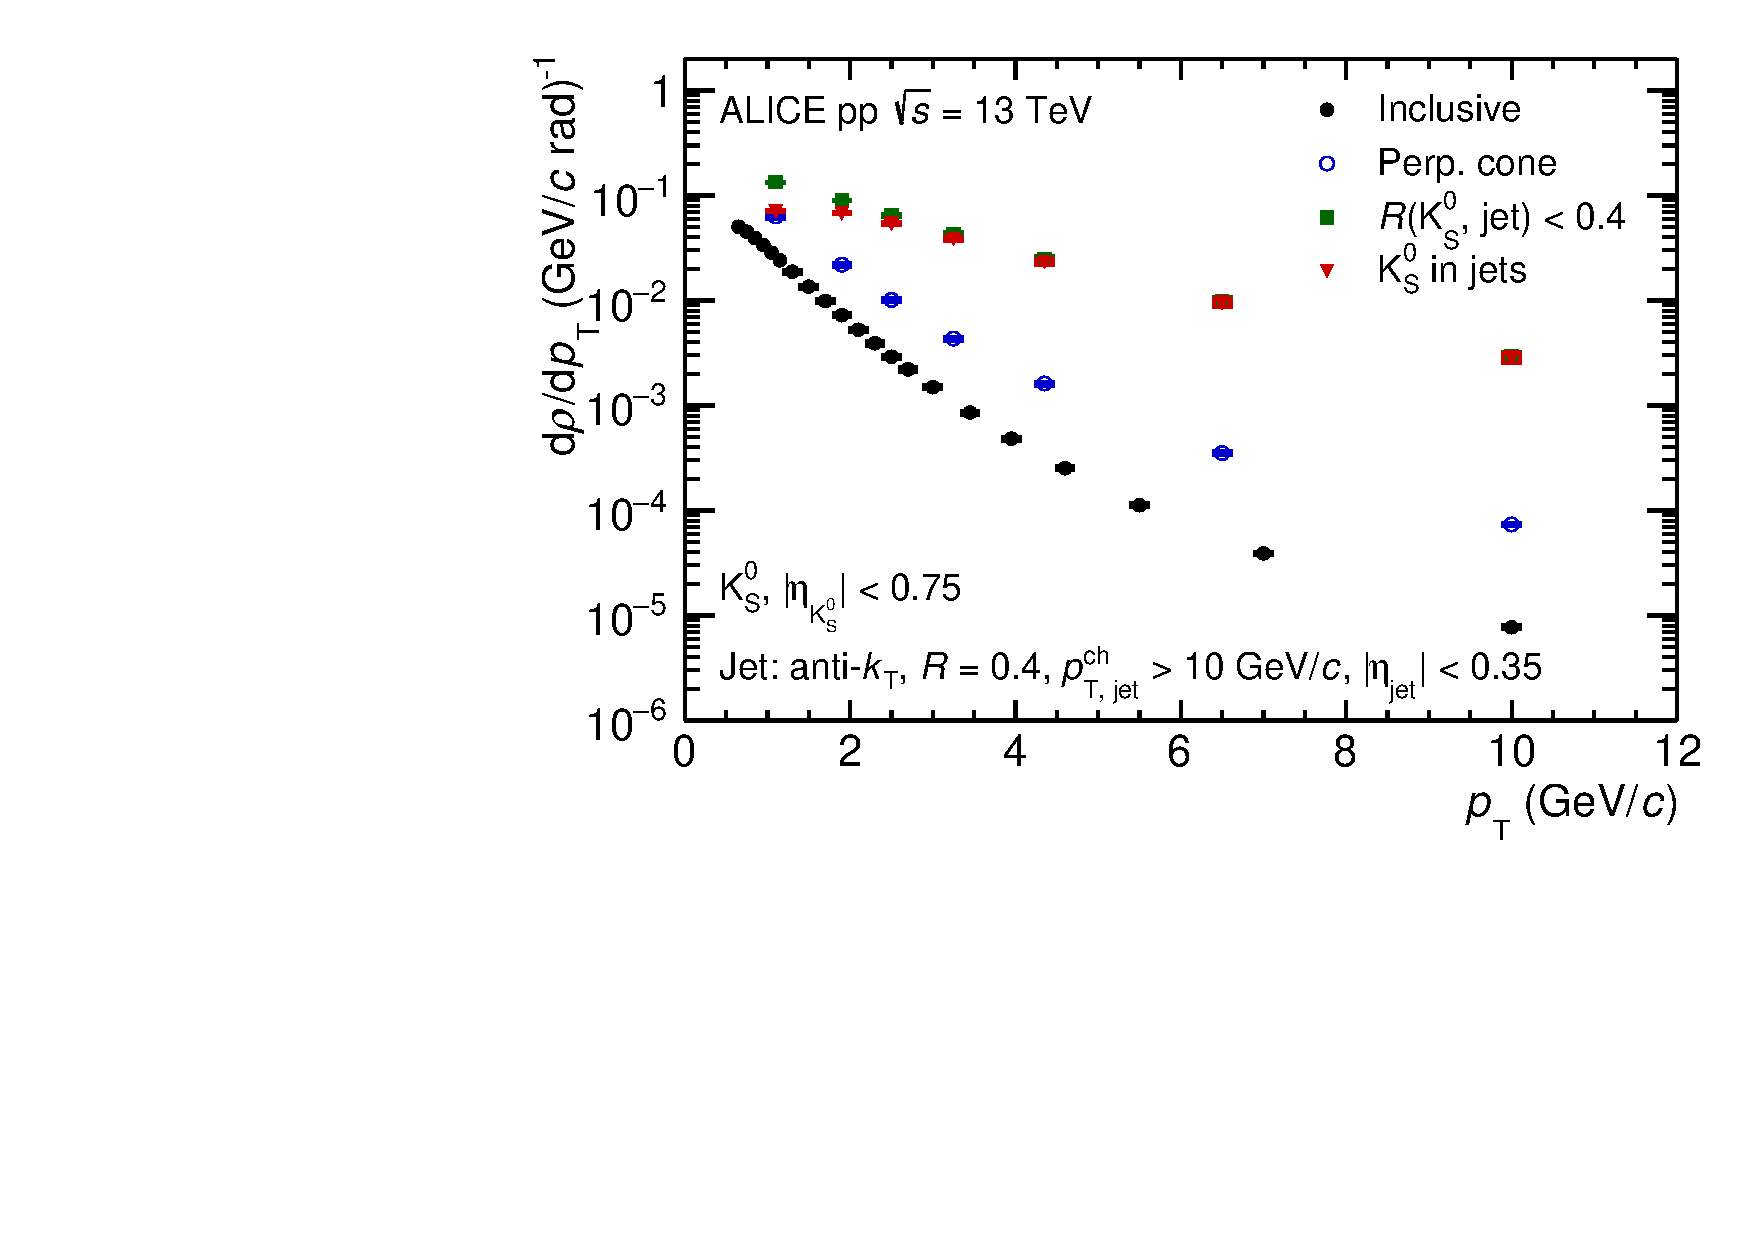
\includegraphics[width=.49\textwidth]{cf04_1}
		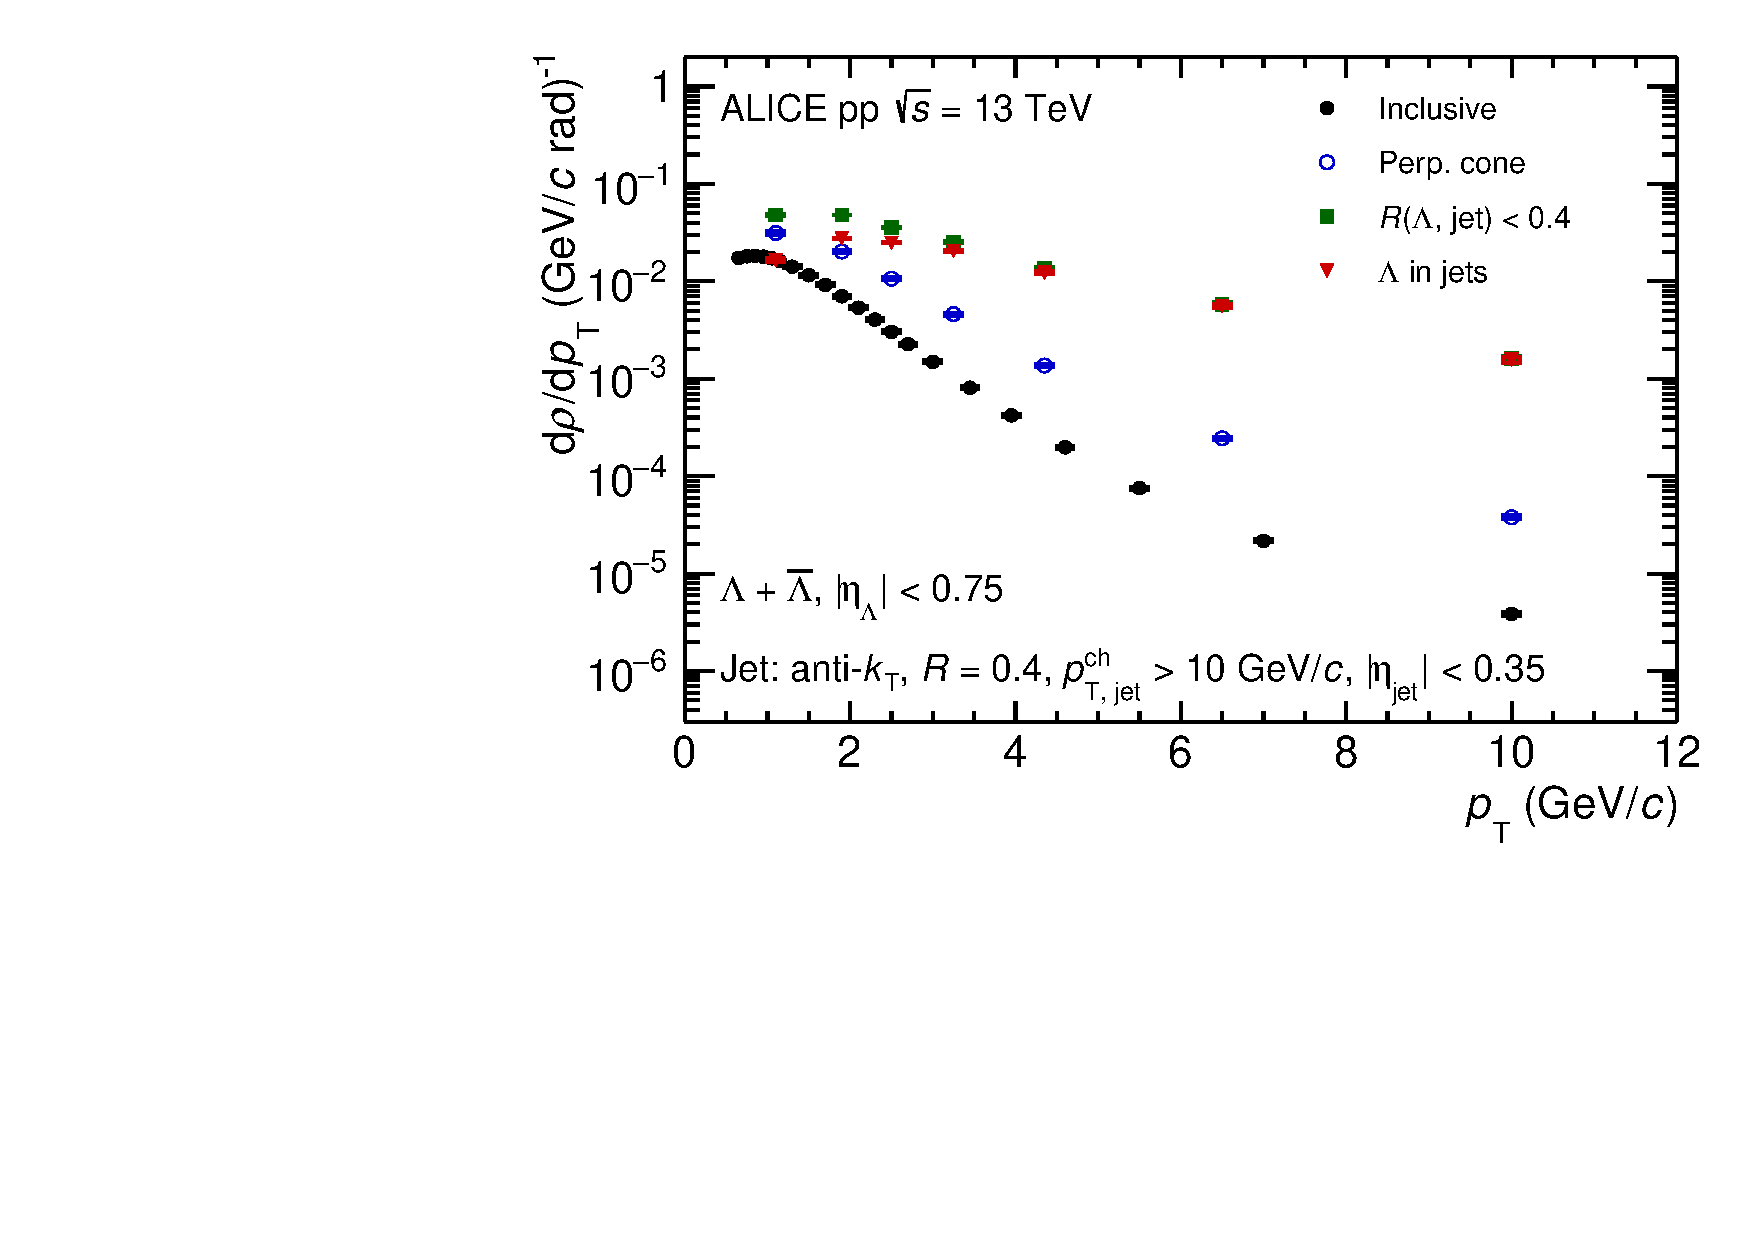
\includegraphics[width=.49\textwidth]{cf04_2}
		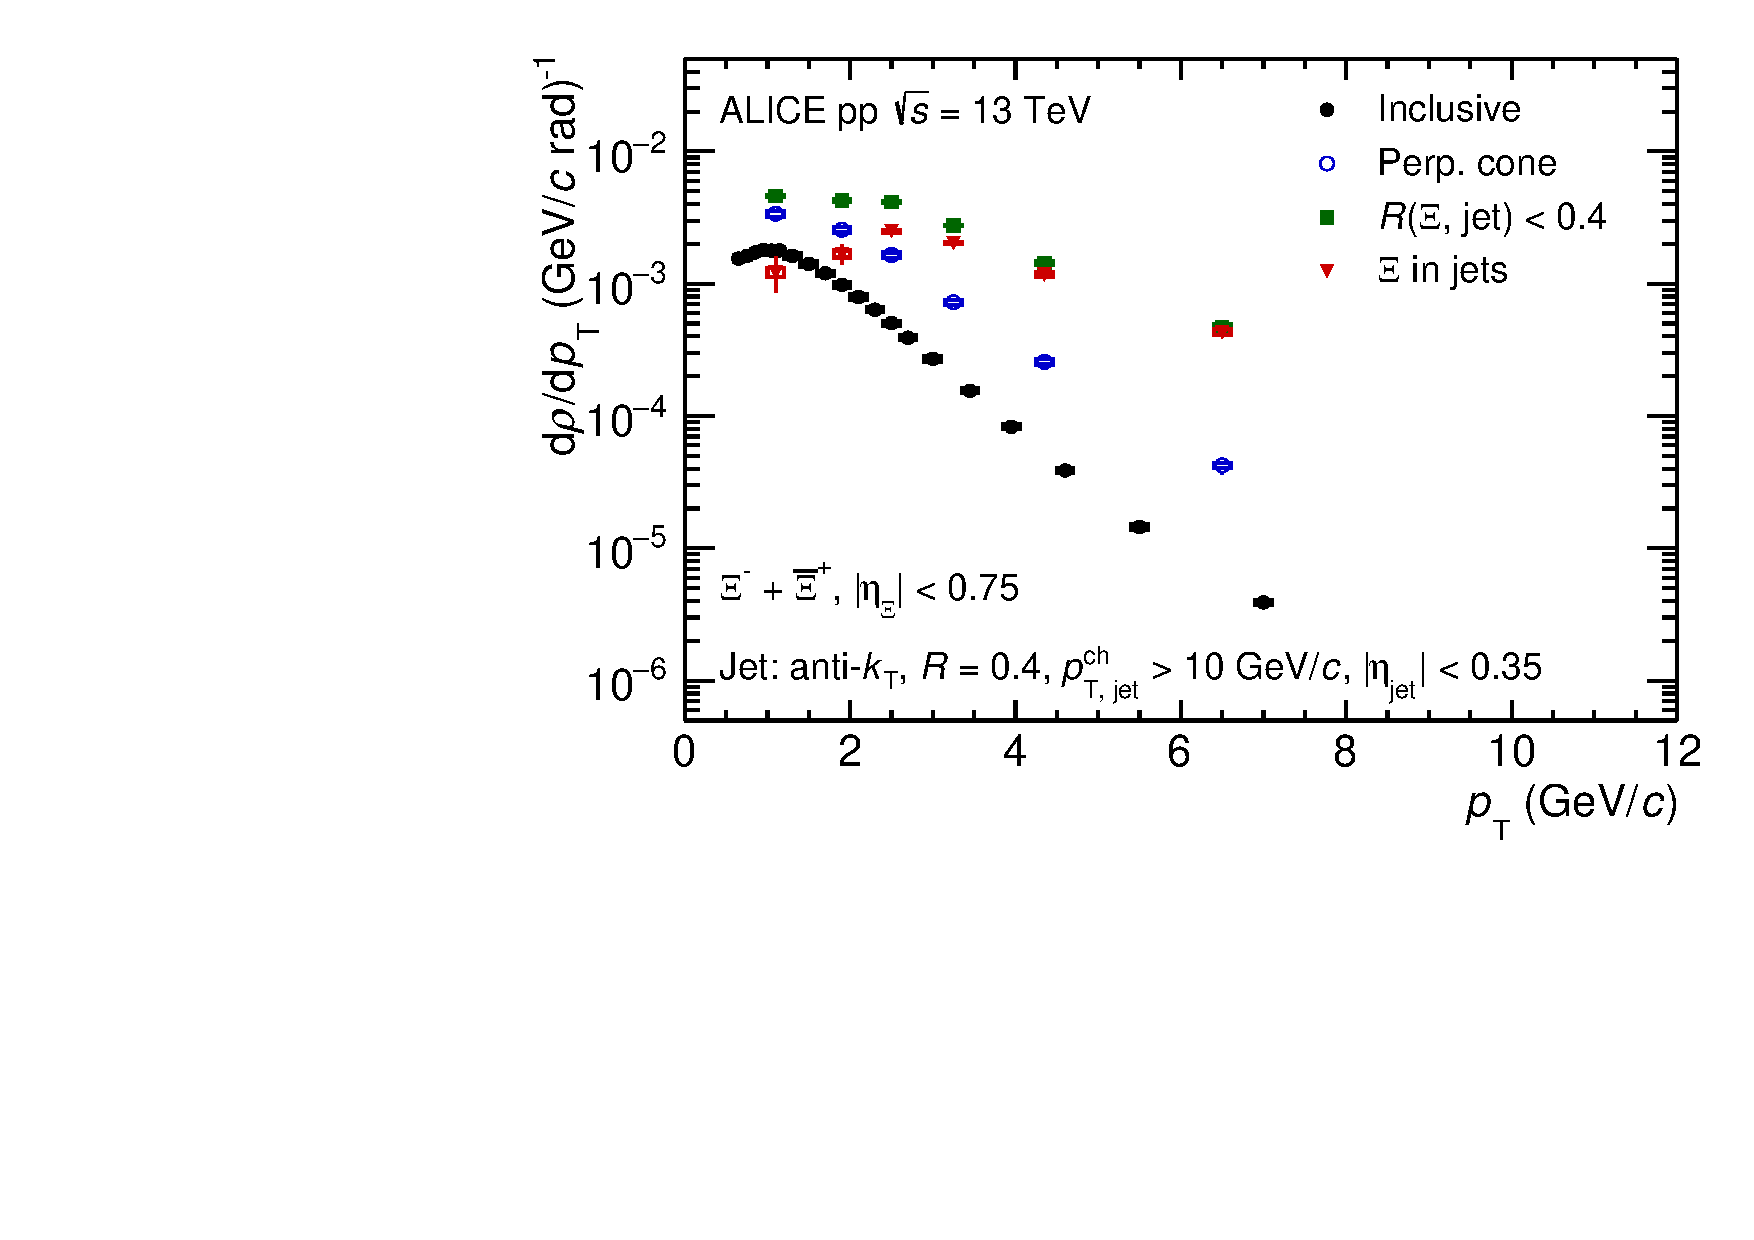
\includegraphics[width=.49\textwidth]{cf04_3}
		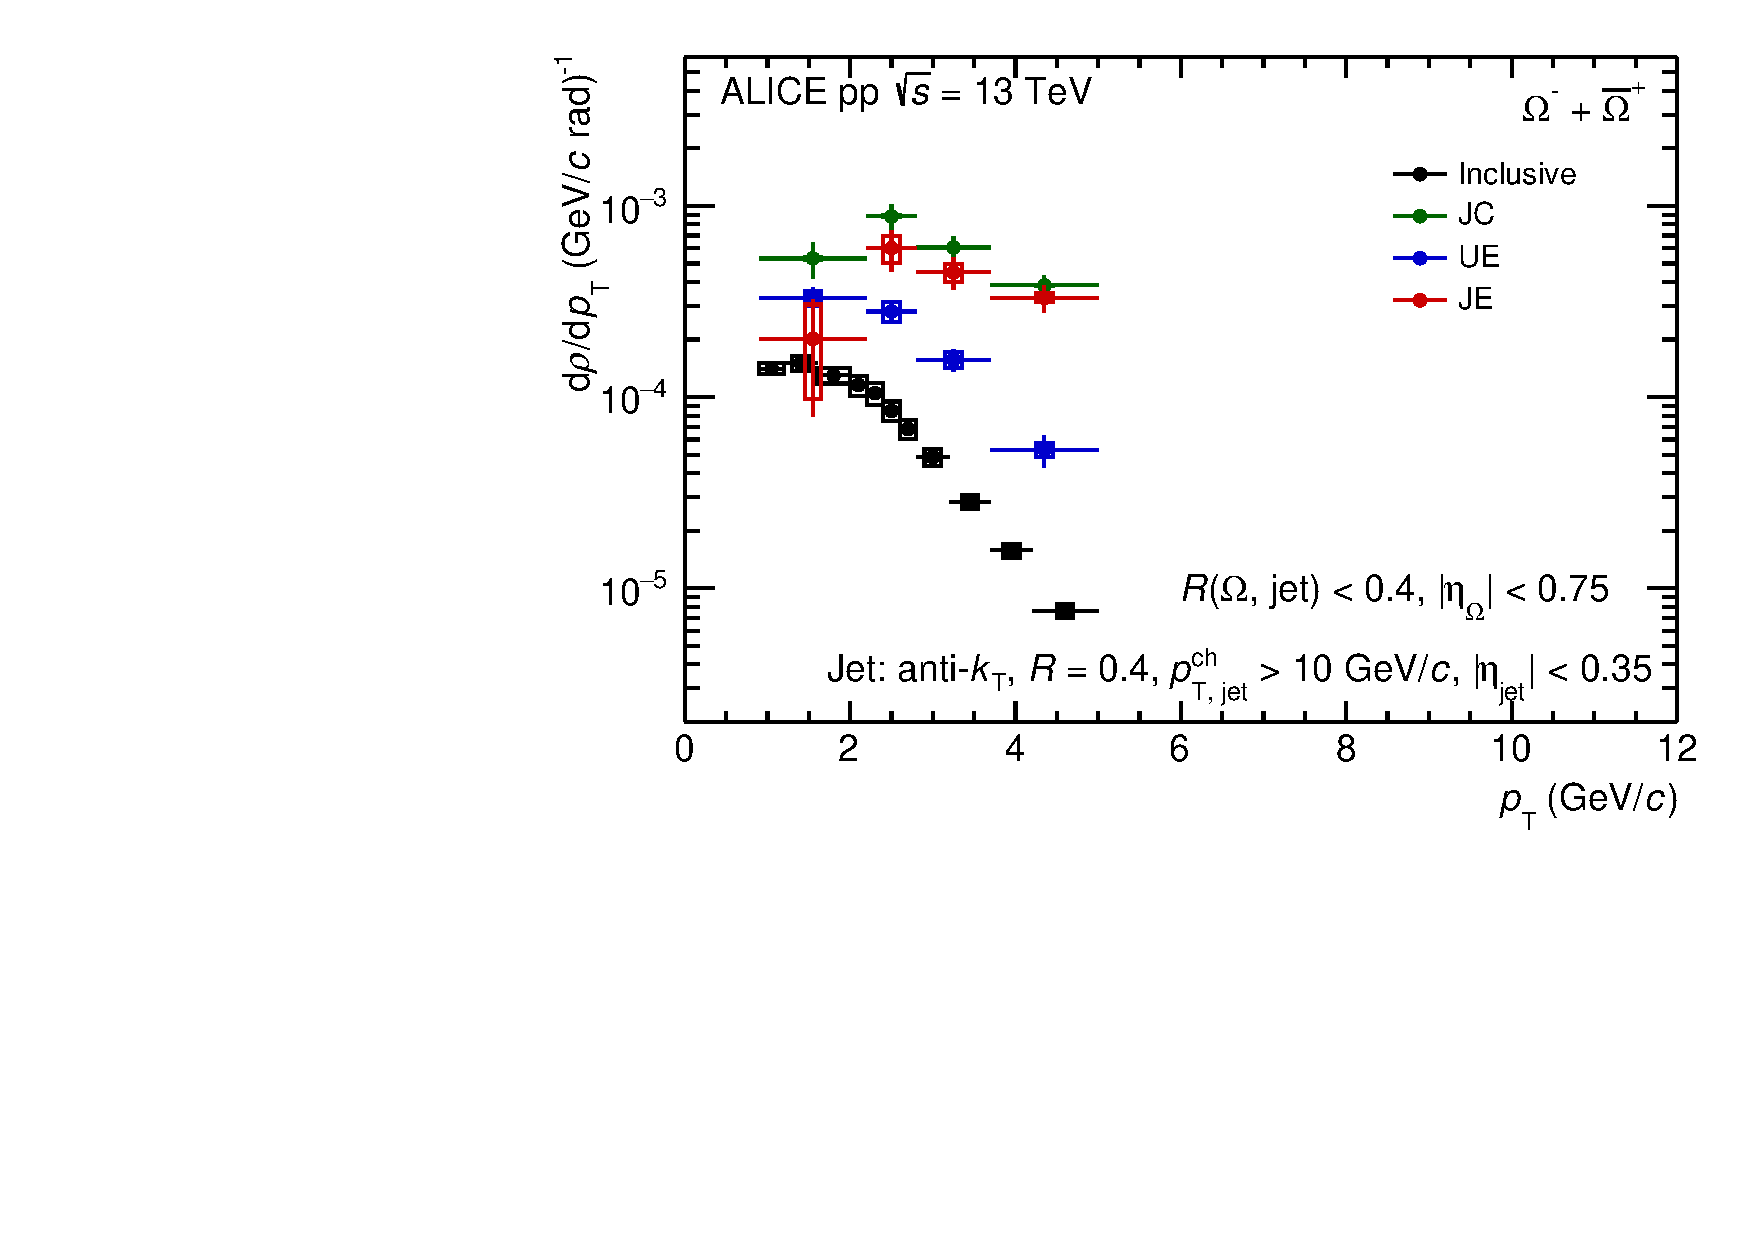
\includegraphics[width=.49\textwidth]{cf04_4}
	\end{center}
	\caption{\DIFaddFL{$\pT$-differential density of $\kzero$, $\lmb + \almb$, $\X + \Ix$ and $\Om + \Mo$ in }\pp \DIFaddFL{collisions at }\thirteen\DIFaddFL{. The black points represent particles from minimum bias events, the green points represent particles from the jet cones, the blue points represent particles within a cone perpendicular to the jet, associated with the underlying event and the red points represent the particle from the jet fragmentation.}}
	\label{fig:ppSpect}
\end{figure}
\begin{figure}[!ht]
	\begin{center}
		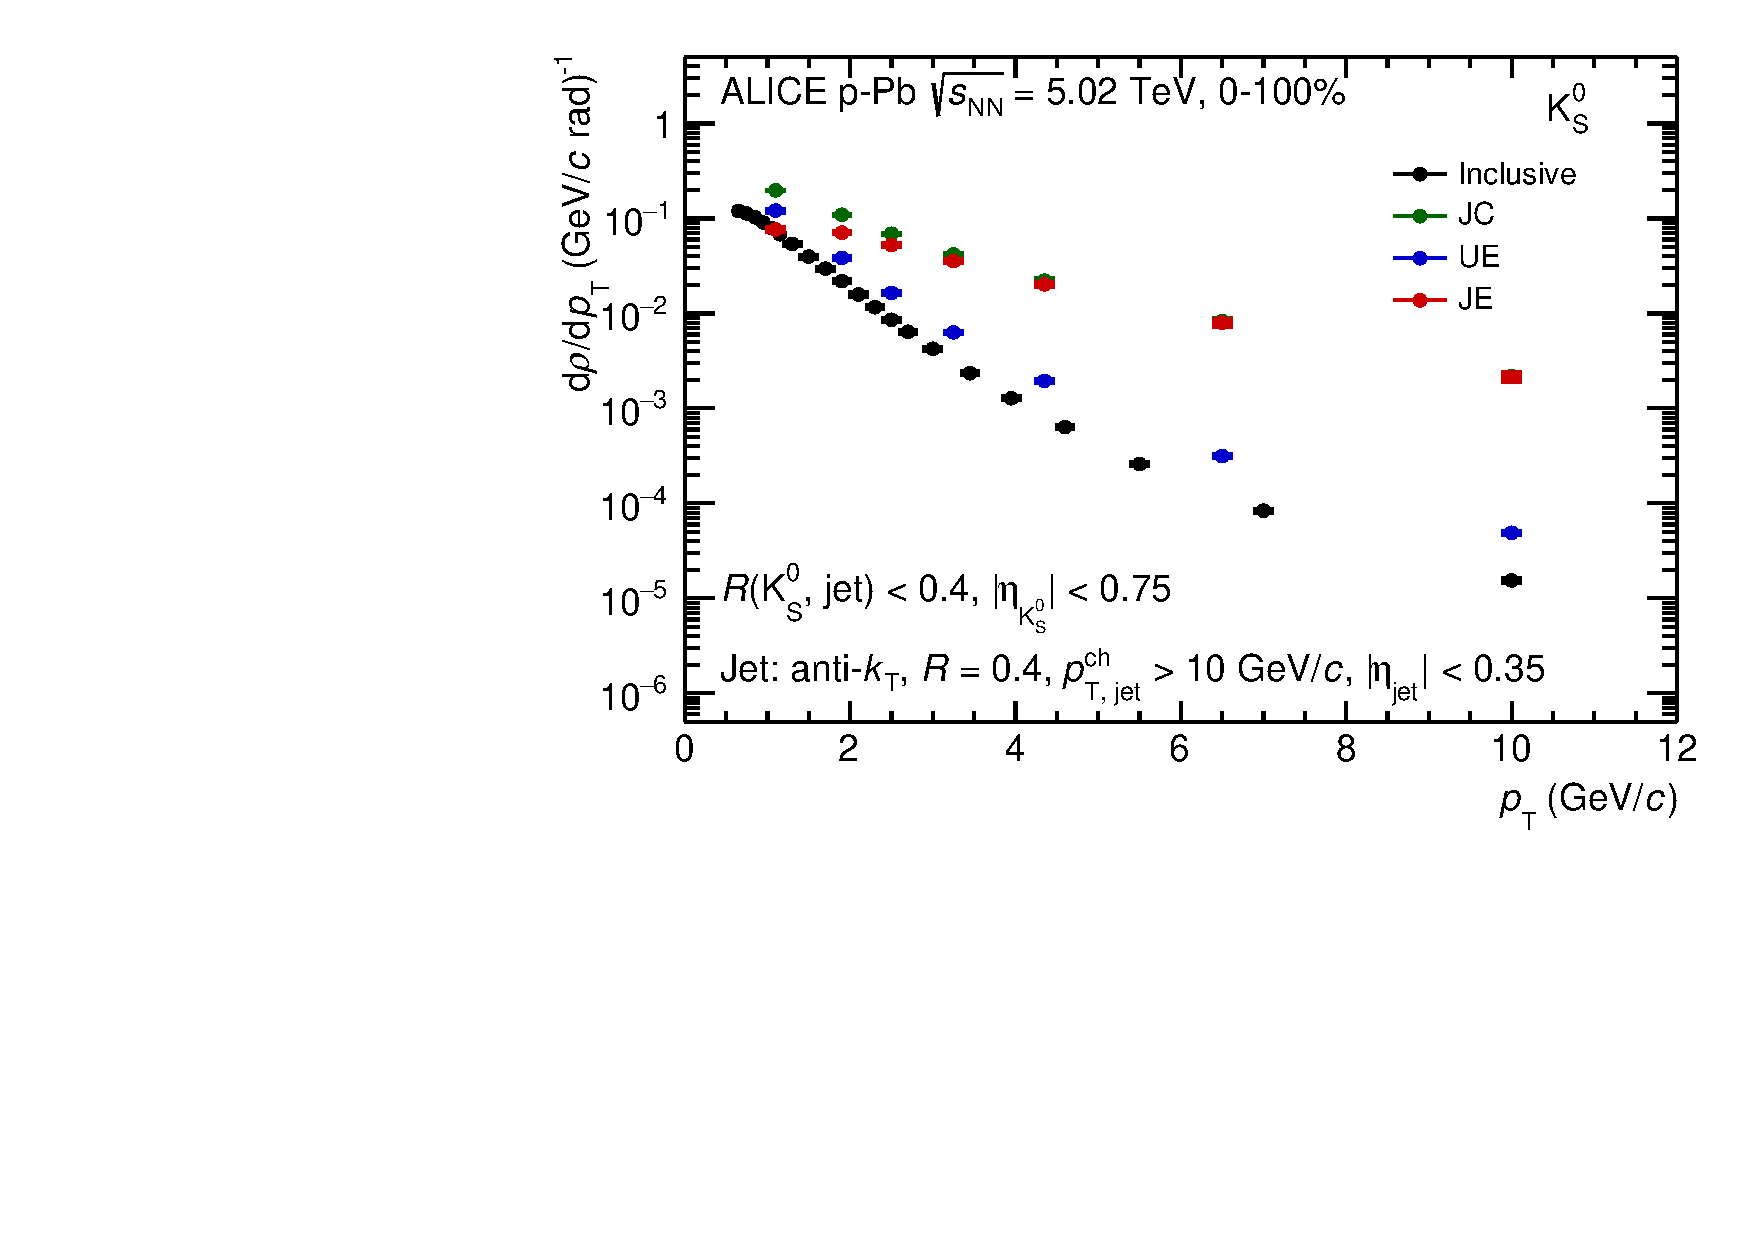
\includegraphics[width=.49\textwidth]{cf05_1}
		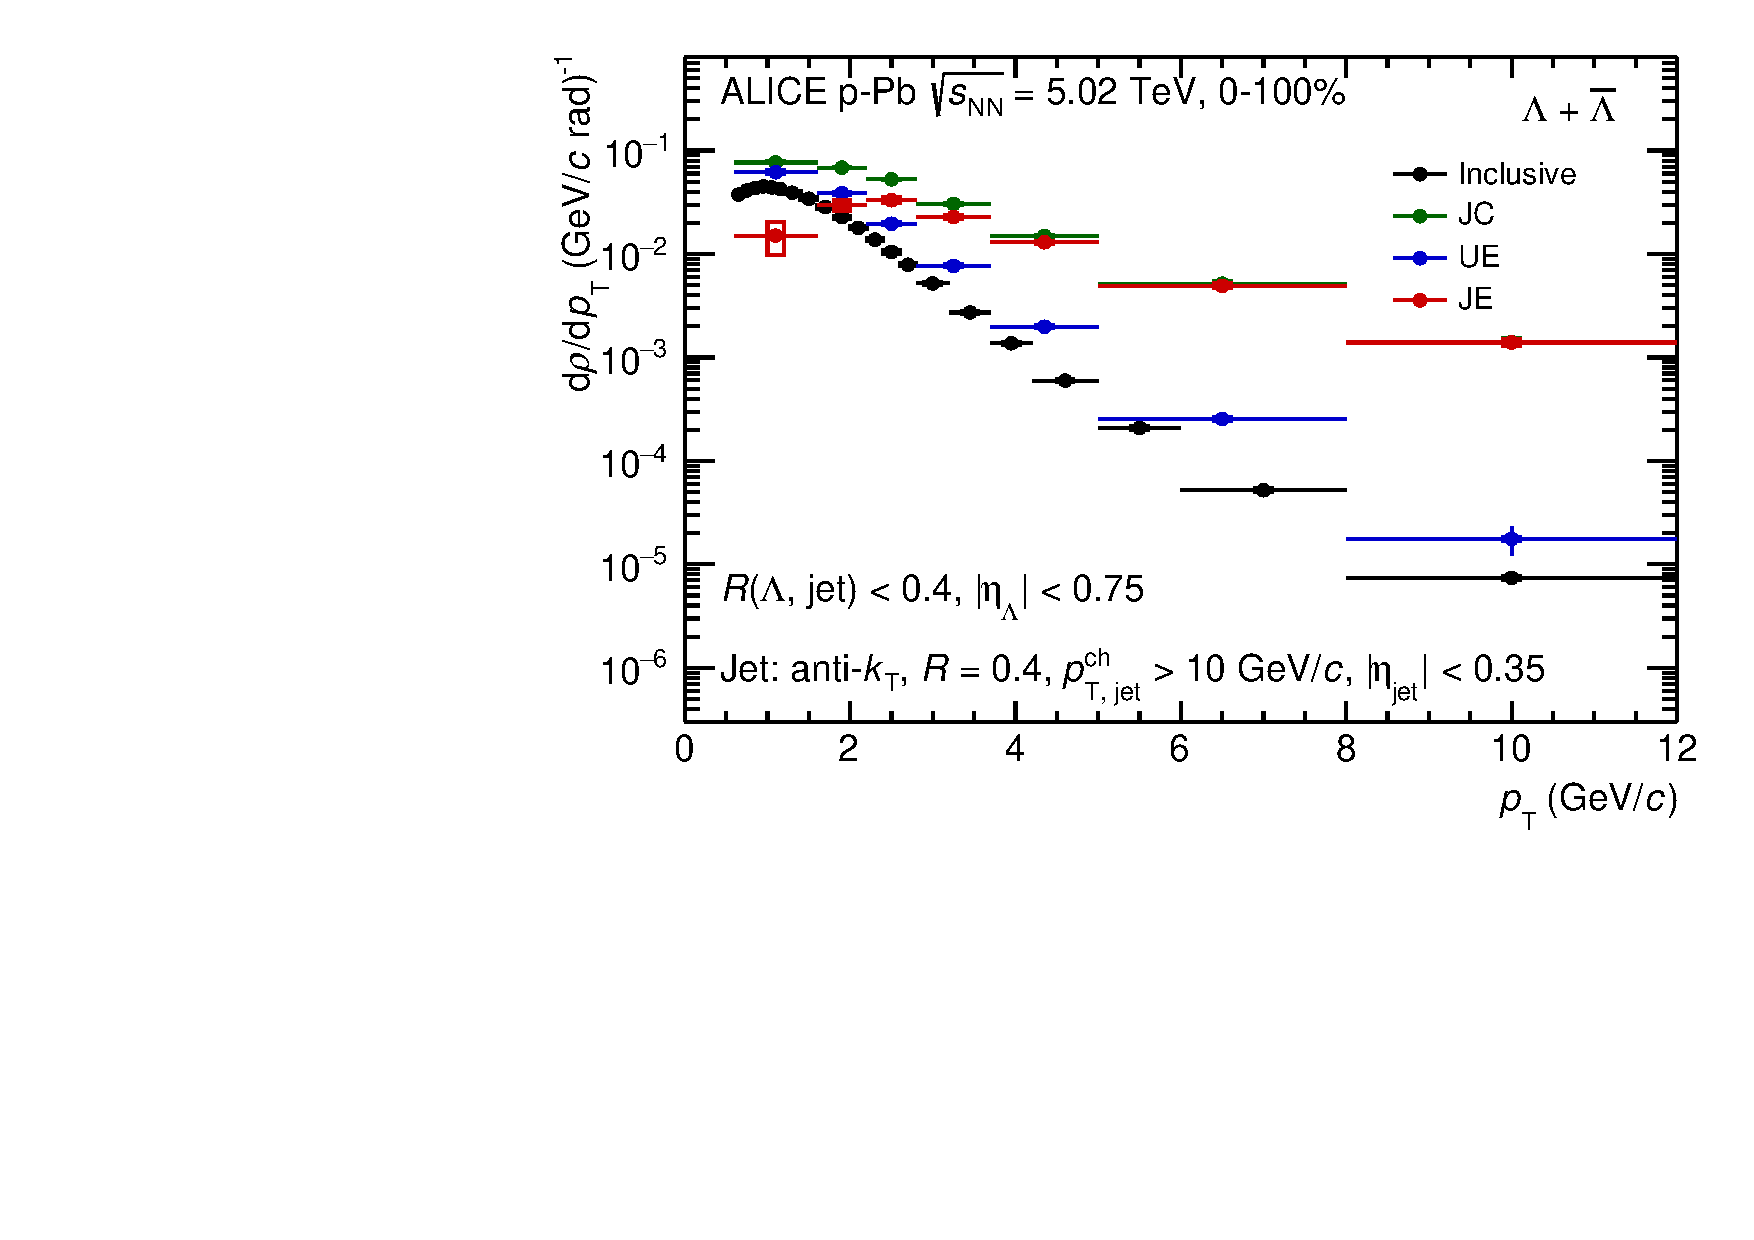
\includegraphics[width=.49\textwidth]{cf05_2}
		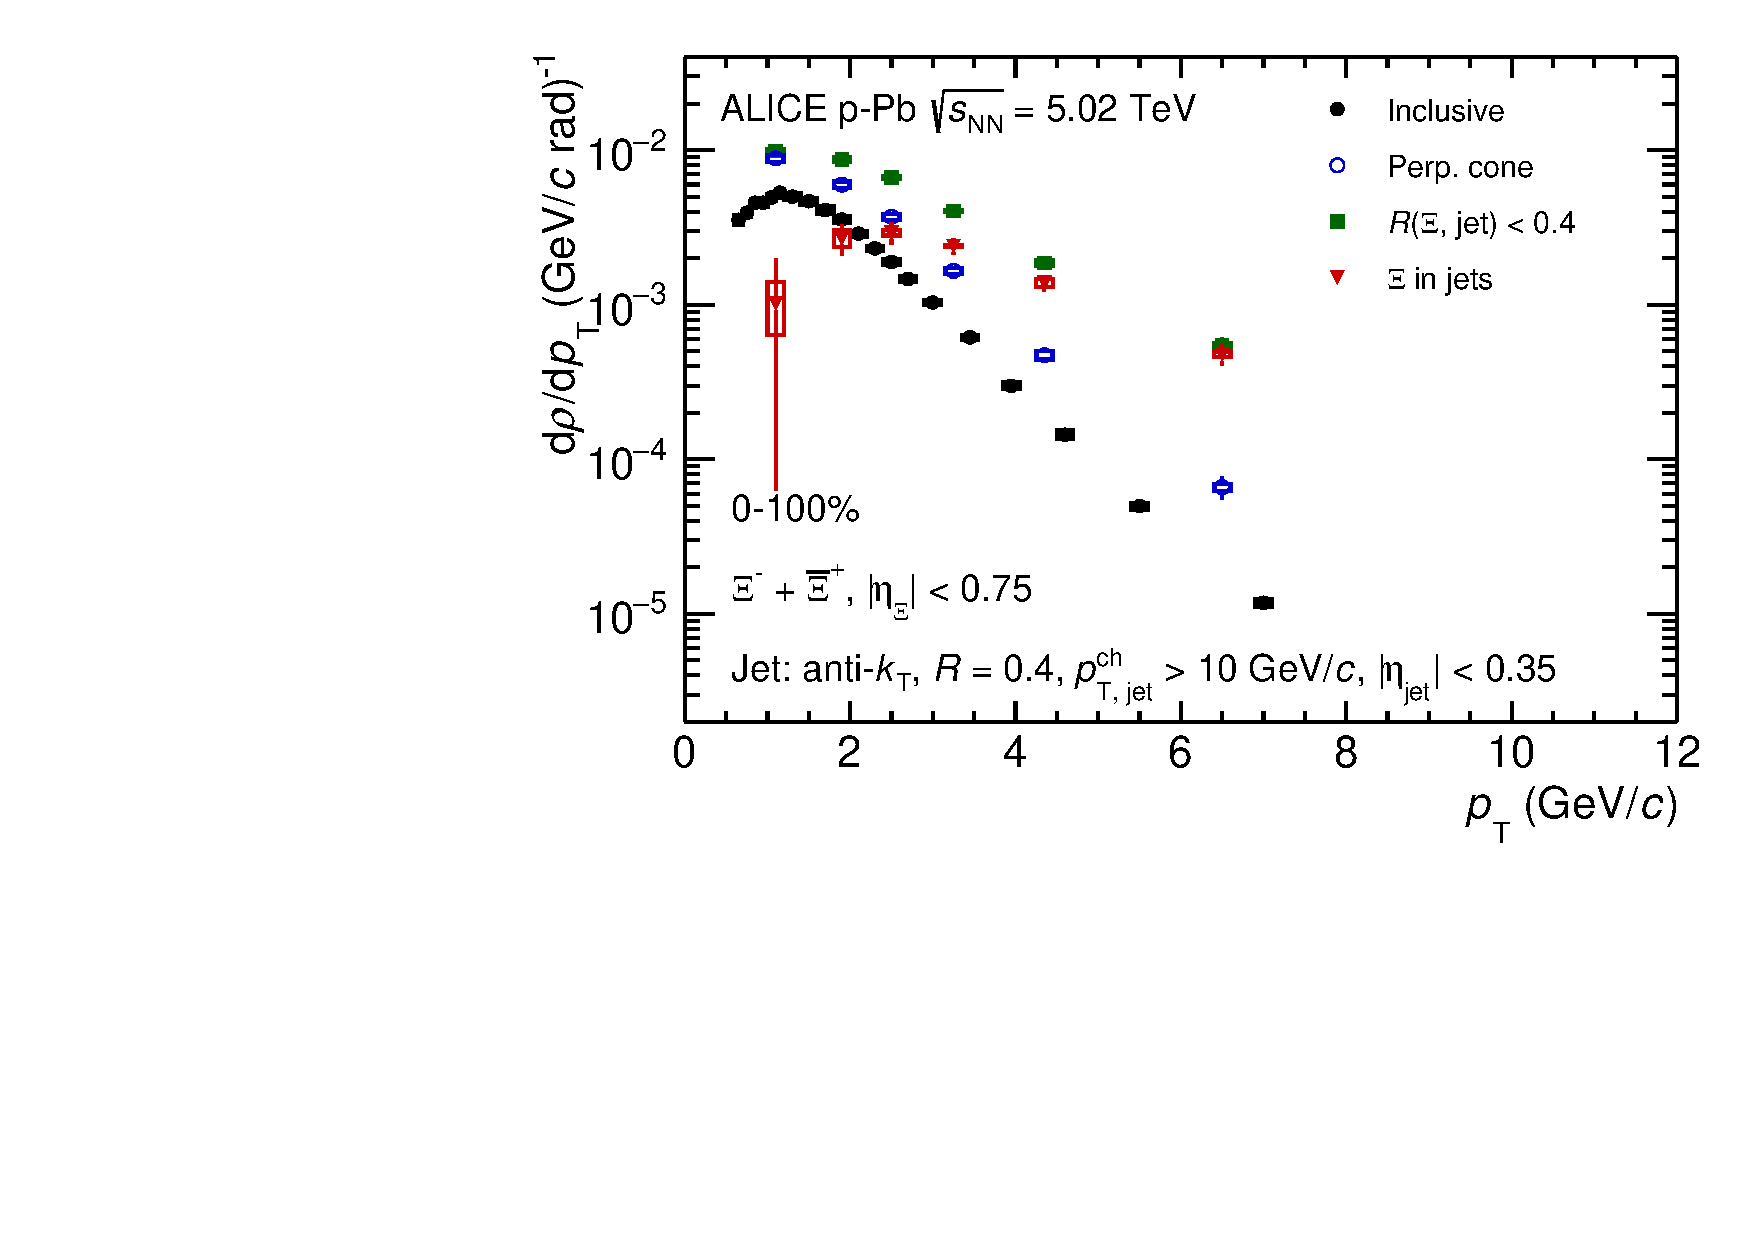
\includegraphics[width=.49\textwidth]{cf05_3}
		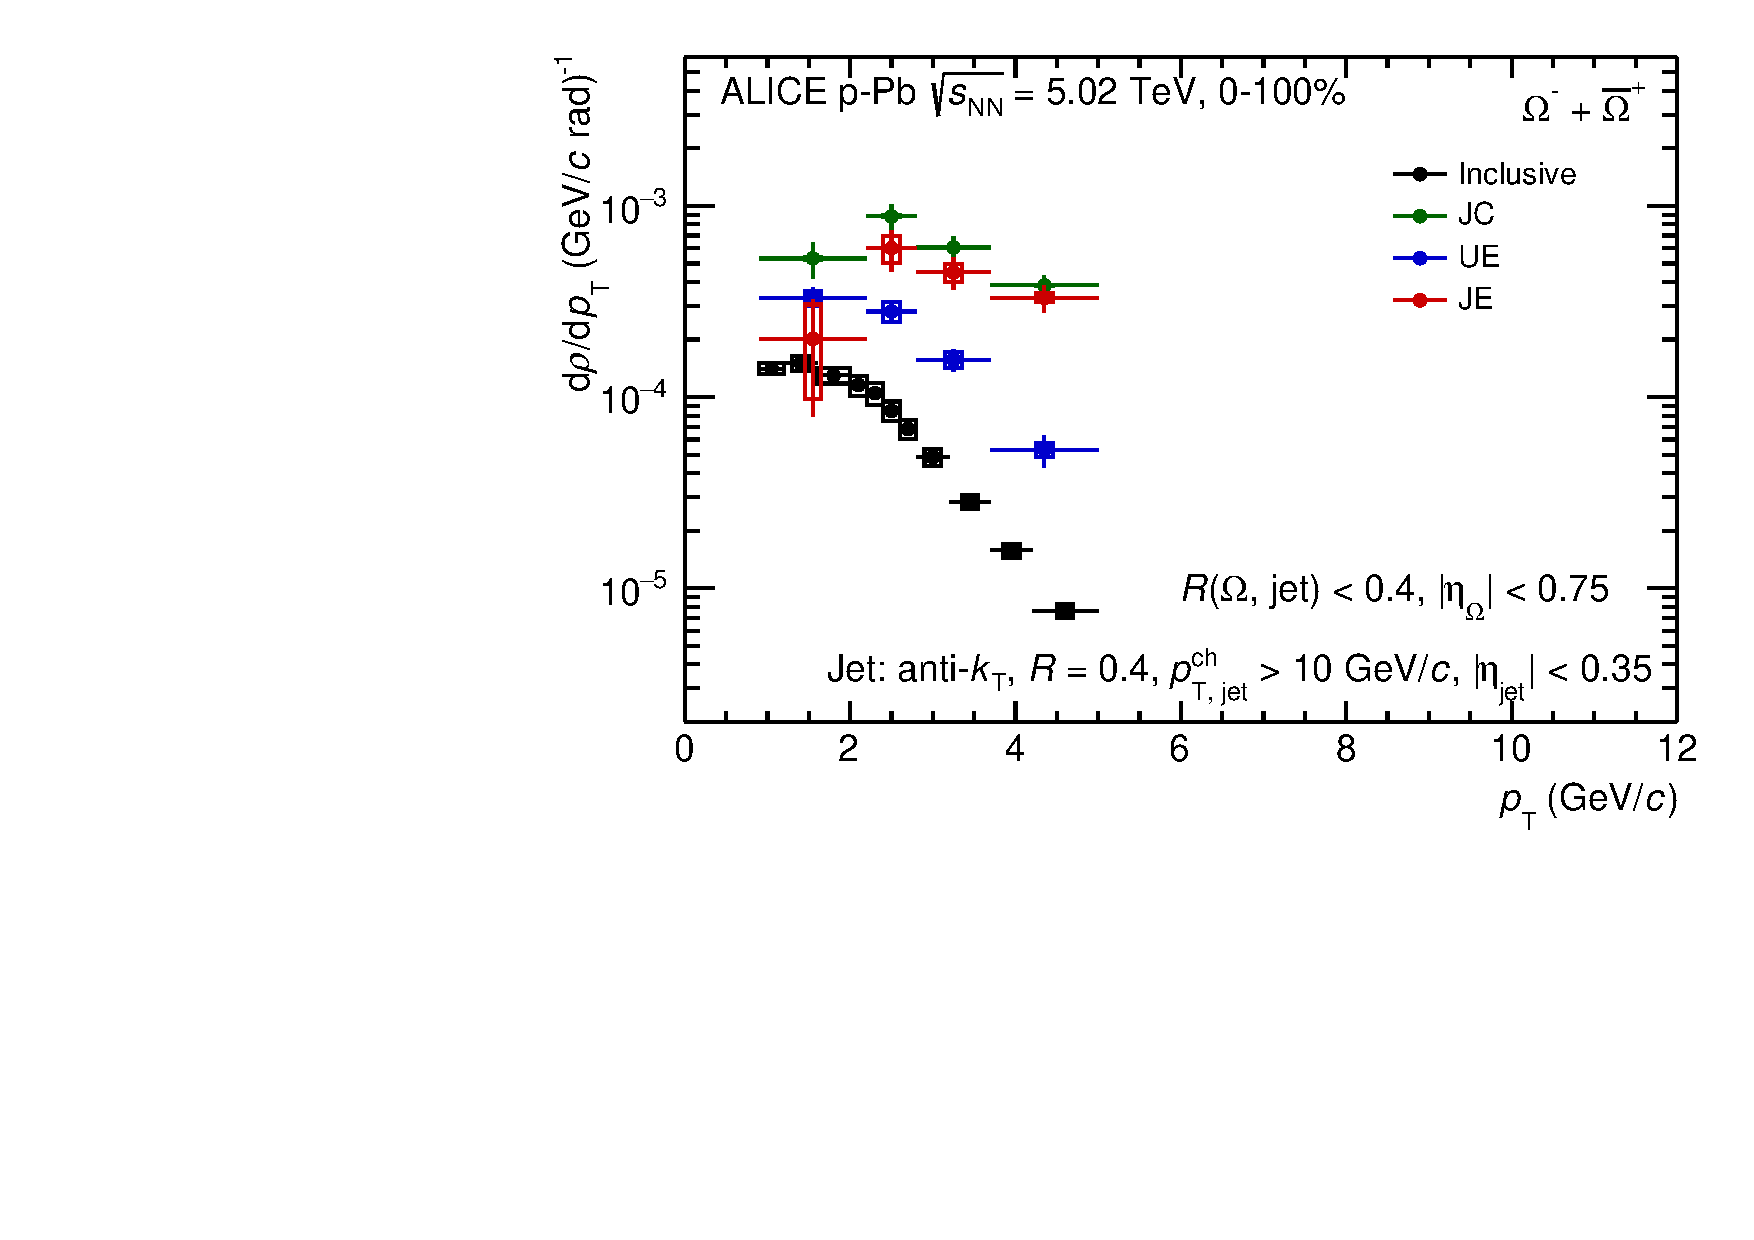
\includegraphics[width=.49\textwidth]{cf05_4}
	\end{center}
	\caption{\DIFaddFL{$\pT$-differential density of $\kzero$, $\lmb + \almb$, $\X + \Ix$ and $\Om + \Mo$ in 0-100\% in }\pPb \DIFaddFL{at }\fivenn\DIFaddFL{. The black points represent particles from minimum bias events, the green points represent particles from the jet cones, the blue points represent particles within a cone perpendicular to the jet, associated with the underlying event and the red points represent the particle from the jet fragmentation.}}
	\label{fig:pPbSpect}
\end{figure}

\DIFadd{The fully corrected }\DIFaddend $\pT$-differential \DIFdelbegin \DIFdel{density }\DIFdelend \DIFaddbegin \DIFadd{densities }\DIFaddend ($\dd \rho/ \dd \pT$ defined by Eq.~\ref{eq:normalize}), for \DIFdelbegin \DIFdel{all particle species}\DIFdelend \DIFaddbegin \kzero\DIFadd{, $\lmb + \almb$, $\X + \Ix$ and $\Om + \Mo$}\DIFaddend , in \pp and MB \pPb collisions are shown in Fig.~\ref{fig:ppSpect} and \ref{fig:pPbSpect}, respectively.
\DIFdelbegin \DIFdel{All the hadrons' densities with }\DIFdelend \DIFaddbegin \DIFadd{The }\DIFaddend $\pT$\DIFdelbegin \DIFdel{are observed to become harder within events that require at least one charged particle jet with $\pTjch > 10$~}%DIFDELCMD < \GeVc%%%
\DIFdel{.
Also,as expected, the particle }\DIFdelend \DIFaddbegin \DIFadd{-differential particle density (d$\rho$/d$\pT$) within charged-particle jets is compared with that of inclusive particles and with perpendicular cone particles.
As expected the $\pT$ dependence of the density of those hadrons within jets,as defined in Eq.~\ref{eq:je}, is considerably less steep than in the case of inclusive particles.
The }\DIFaddend $\pT$-differential density \DIFdelbegin \DIFdel{in jet is harder than that in underlying events}\DIFdelend \DIFaddbegin \DIFadd{distribution of inclusive hadrons is lower than that of the PC selection since the latter are obtained from events contain jets with $\pTjch > 10$~}\GeVc\DIFadd{.
At the high-$\pT$ ($\pT > 4$~}\GeVc\DIFadd{) region, the density of particle within charged-particle jets is consistent with the one in jet cone (without the underlying event subtraction).
This is consistent with the expectation that the high-$\pT$ particles originate from jet fragmentation}\DIFaddend . 

\DIFdelbegin %DIFDELCMD < \begin{figure}[!ht]
%DIFDELCMD < 	\begin{center}
%DIFDELCMD < 		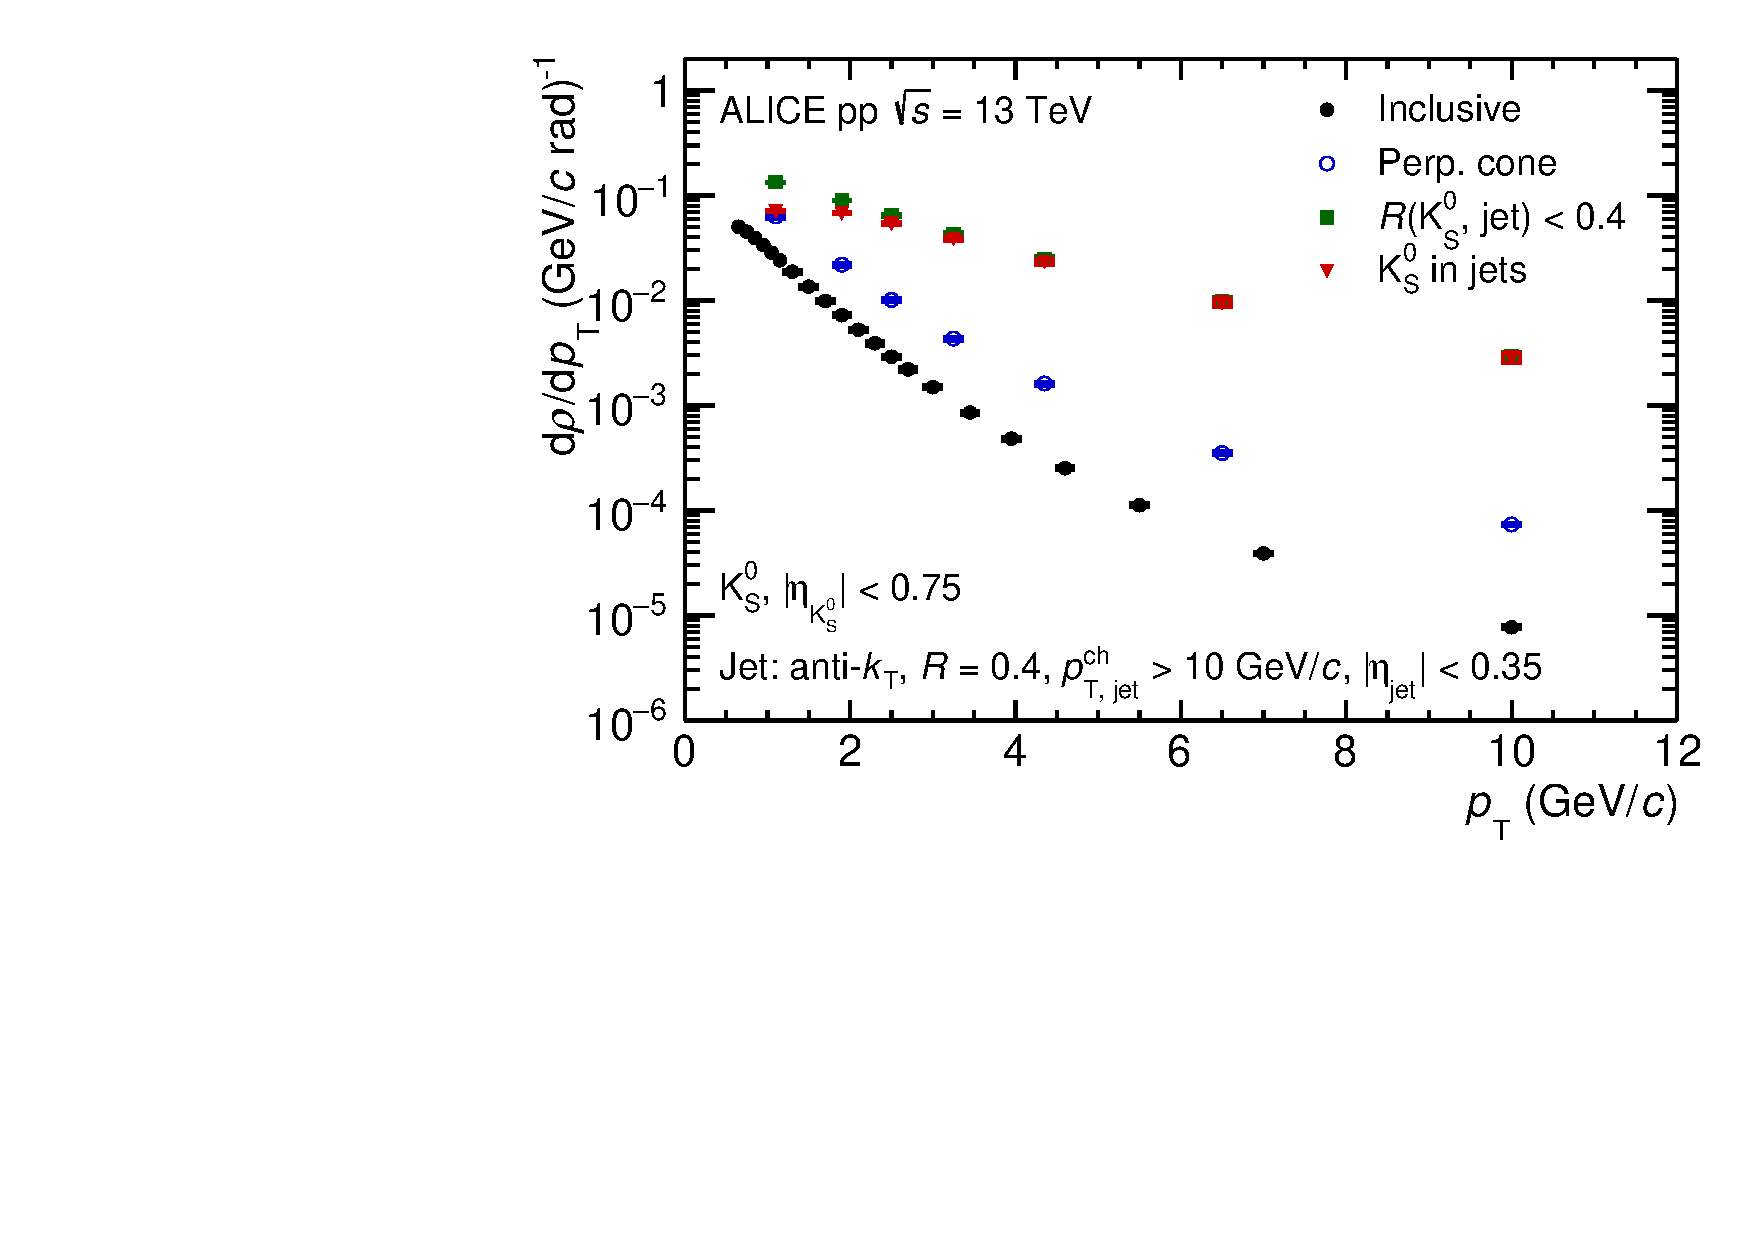
\includegraphics[width=.4\textwidth]{cf04_1}
%DIFDELCMD < 		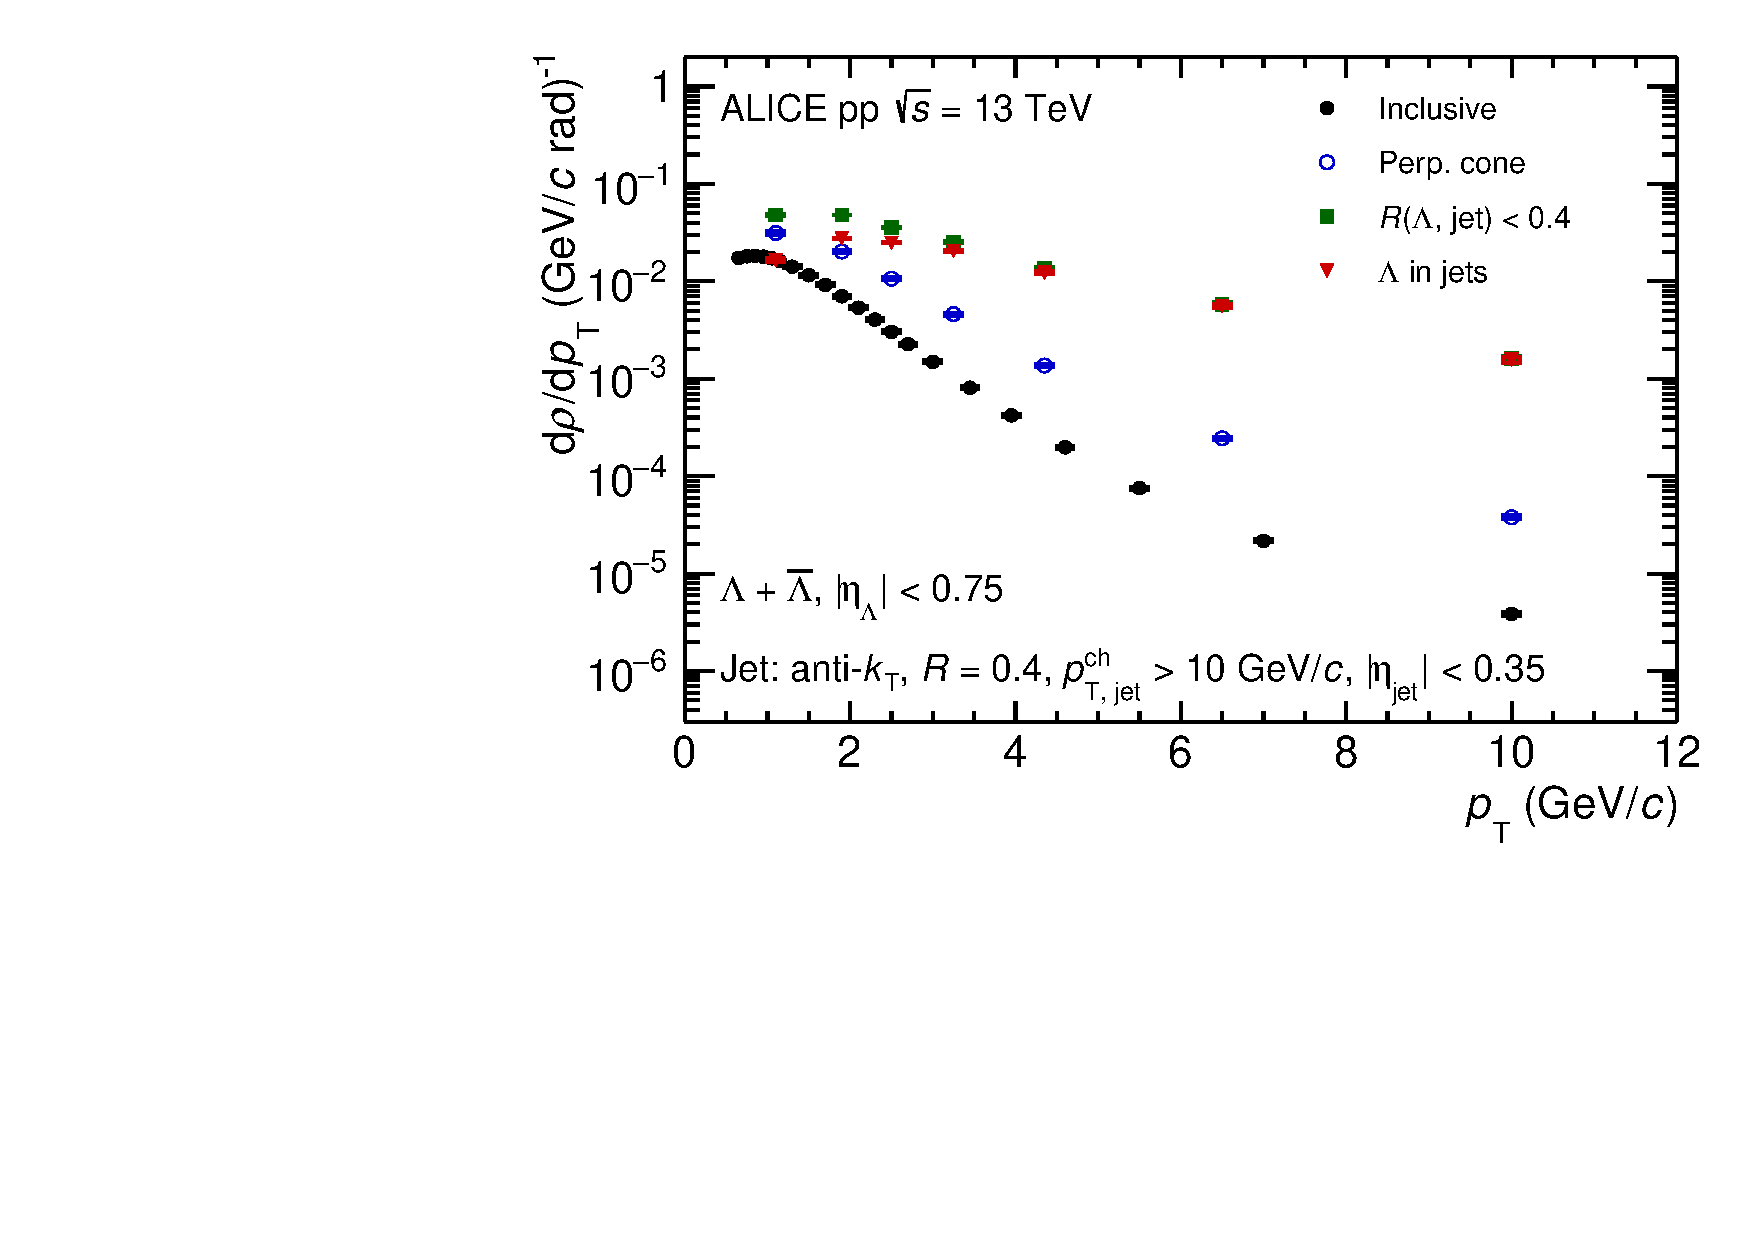
\includegraphics[width=.4\textwidth]{cf04_2}
%DIFDELCMD < 		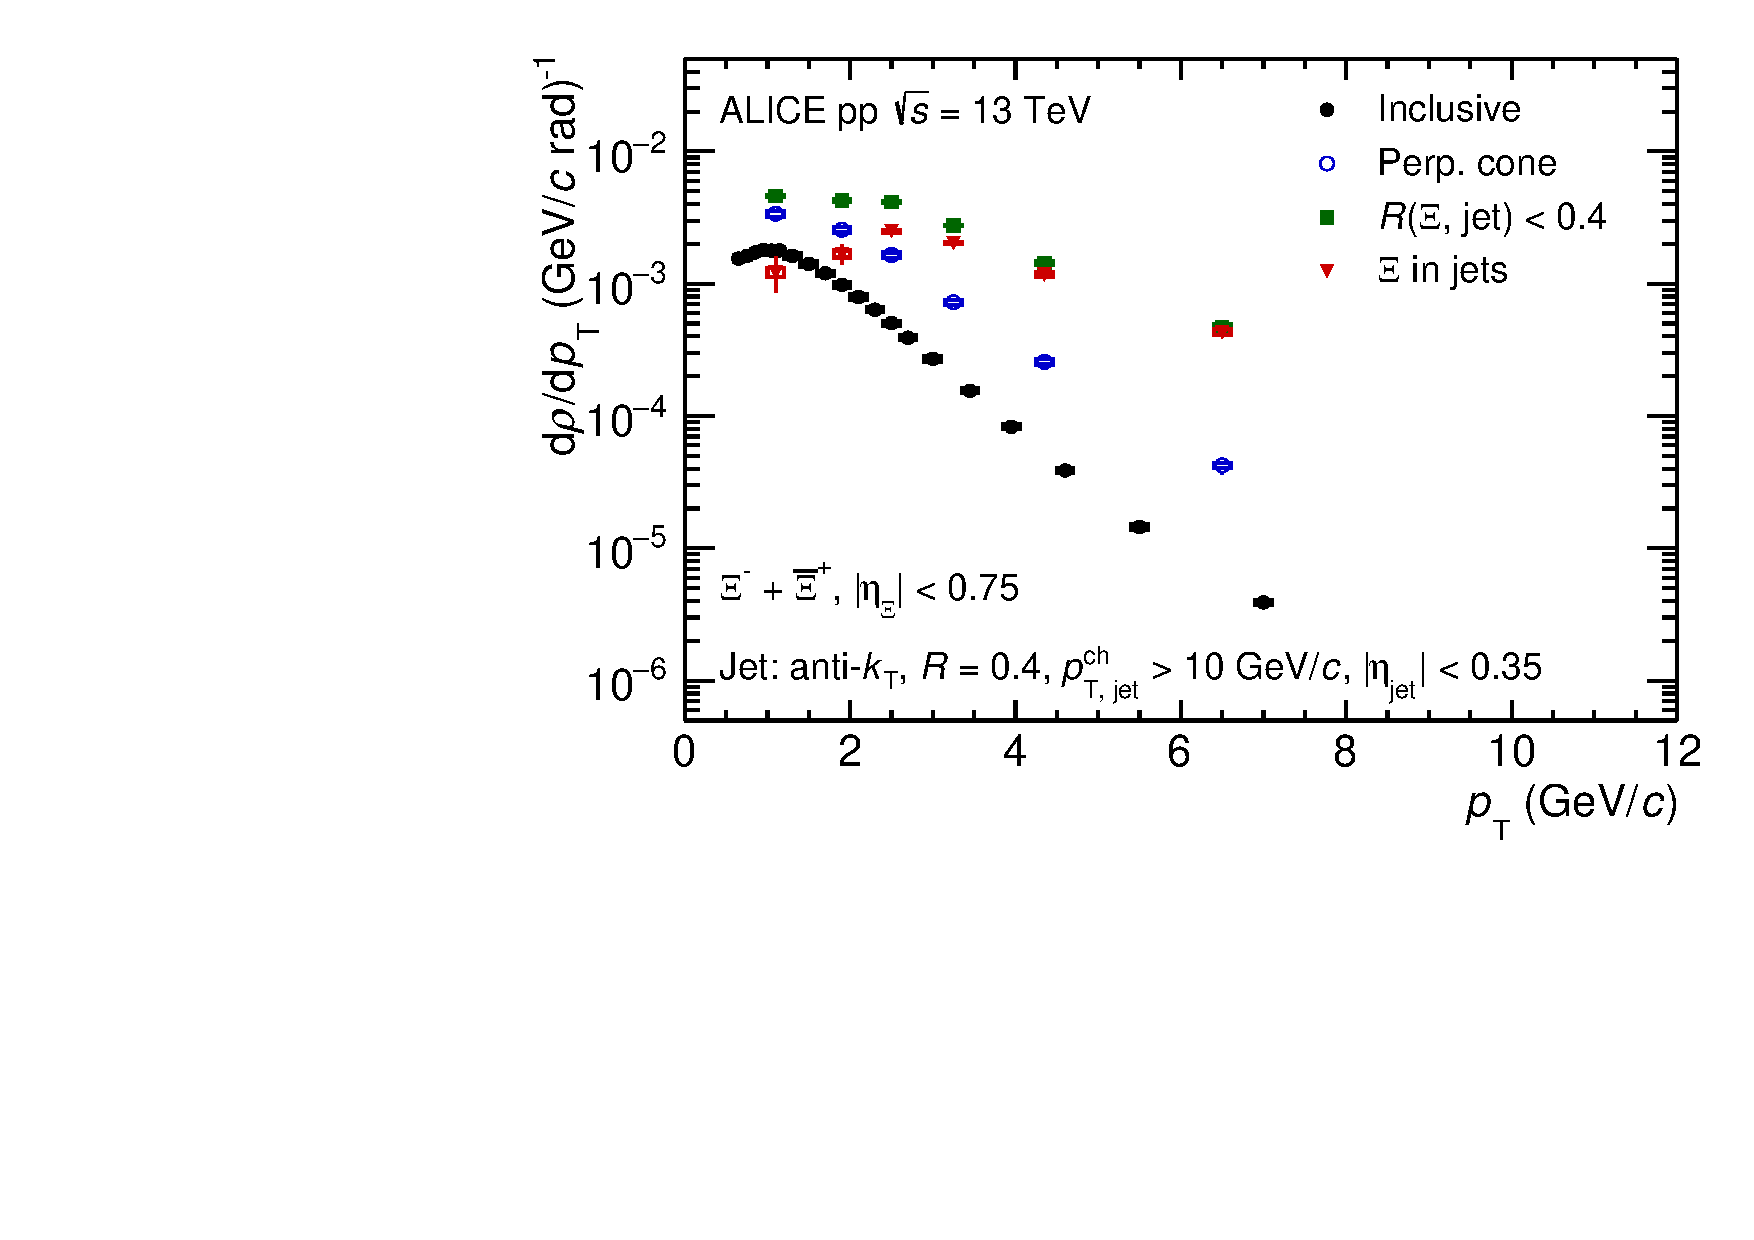
\includegraphics[width=.4\textwidth]{cf04_3}
%DIFDELCMD < 		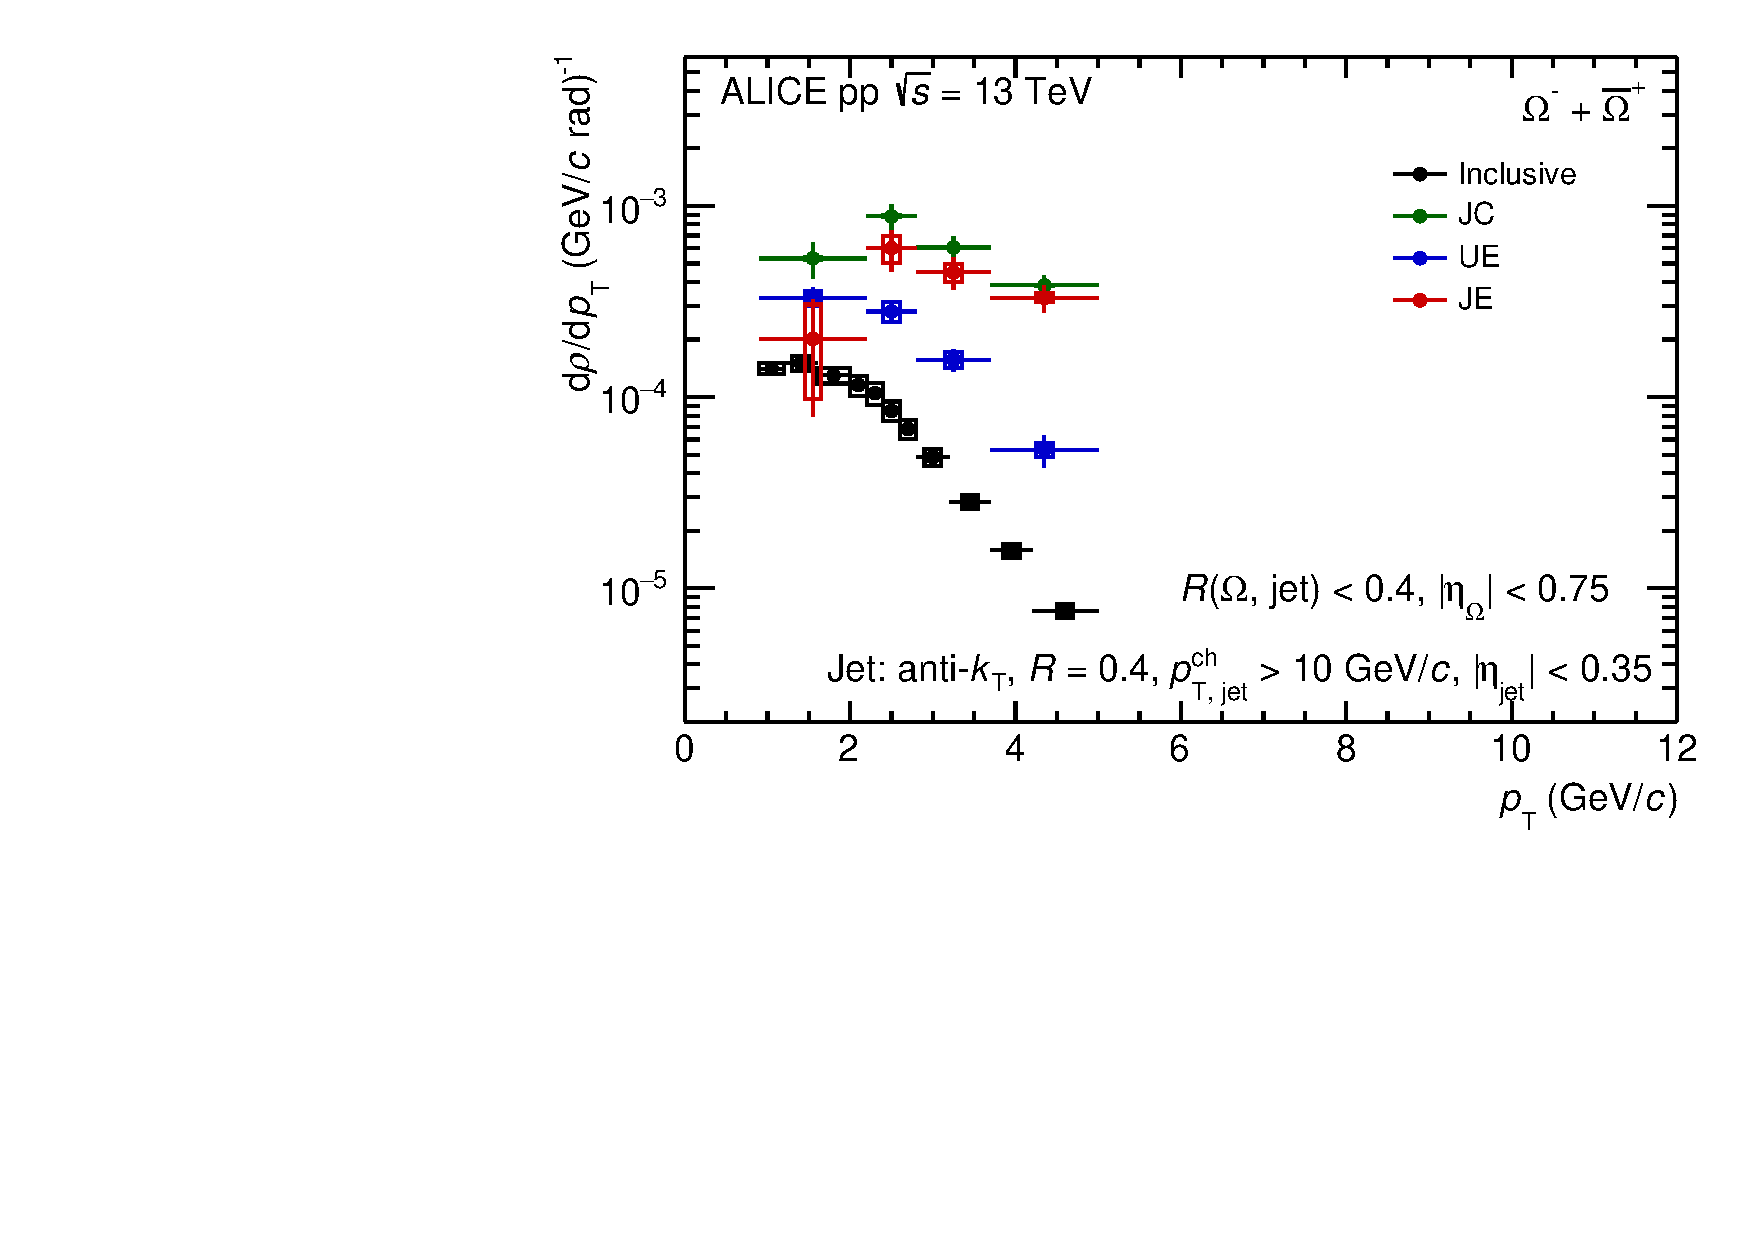
\includegraphics[width=.4\textwidth]{cf04_4}
%DIFDELCMD < 	\end{center}
%DIFDELCMD < 	%%%
%DIFDELCMD < \caption{%
{%DIFAUXCMD
\DIFdelFL{$\pT$-differential density of $\kzero$, $\lmb + \almb$, $\X + \Ix$ and $\Om + \Mo$ in }%DIFDELCMD < \pp %%%
\DIFdelFL{at }%DIFDELCMD < \thirteen%%%
\DIFdelFL{. In those plots, the black point represent particles witch from minimum bias events, the green point represent particles which from the jet cones, the blue point represent particles within perpendicular cone of jet which associated with the underlying event and the red point represent the particle from the jet fragmentation.}}
	%DIFAUXCMD
%DIFDELCMD < \label{fig:ppSpect}
%DIFDELCMD < \end{figure}
%DIFDELCMD < \begin{figure}[!ht]
%DIFDELCMD < 	\begin{center}
%DIFDELCMD < 		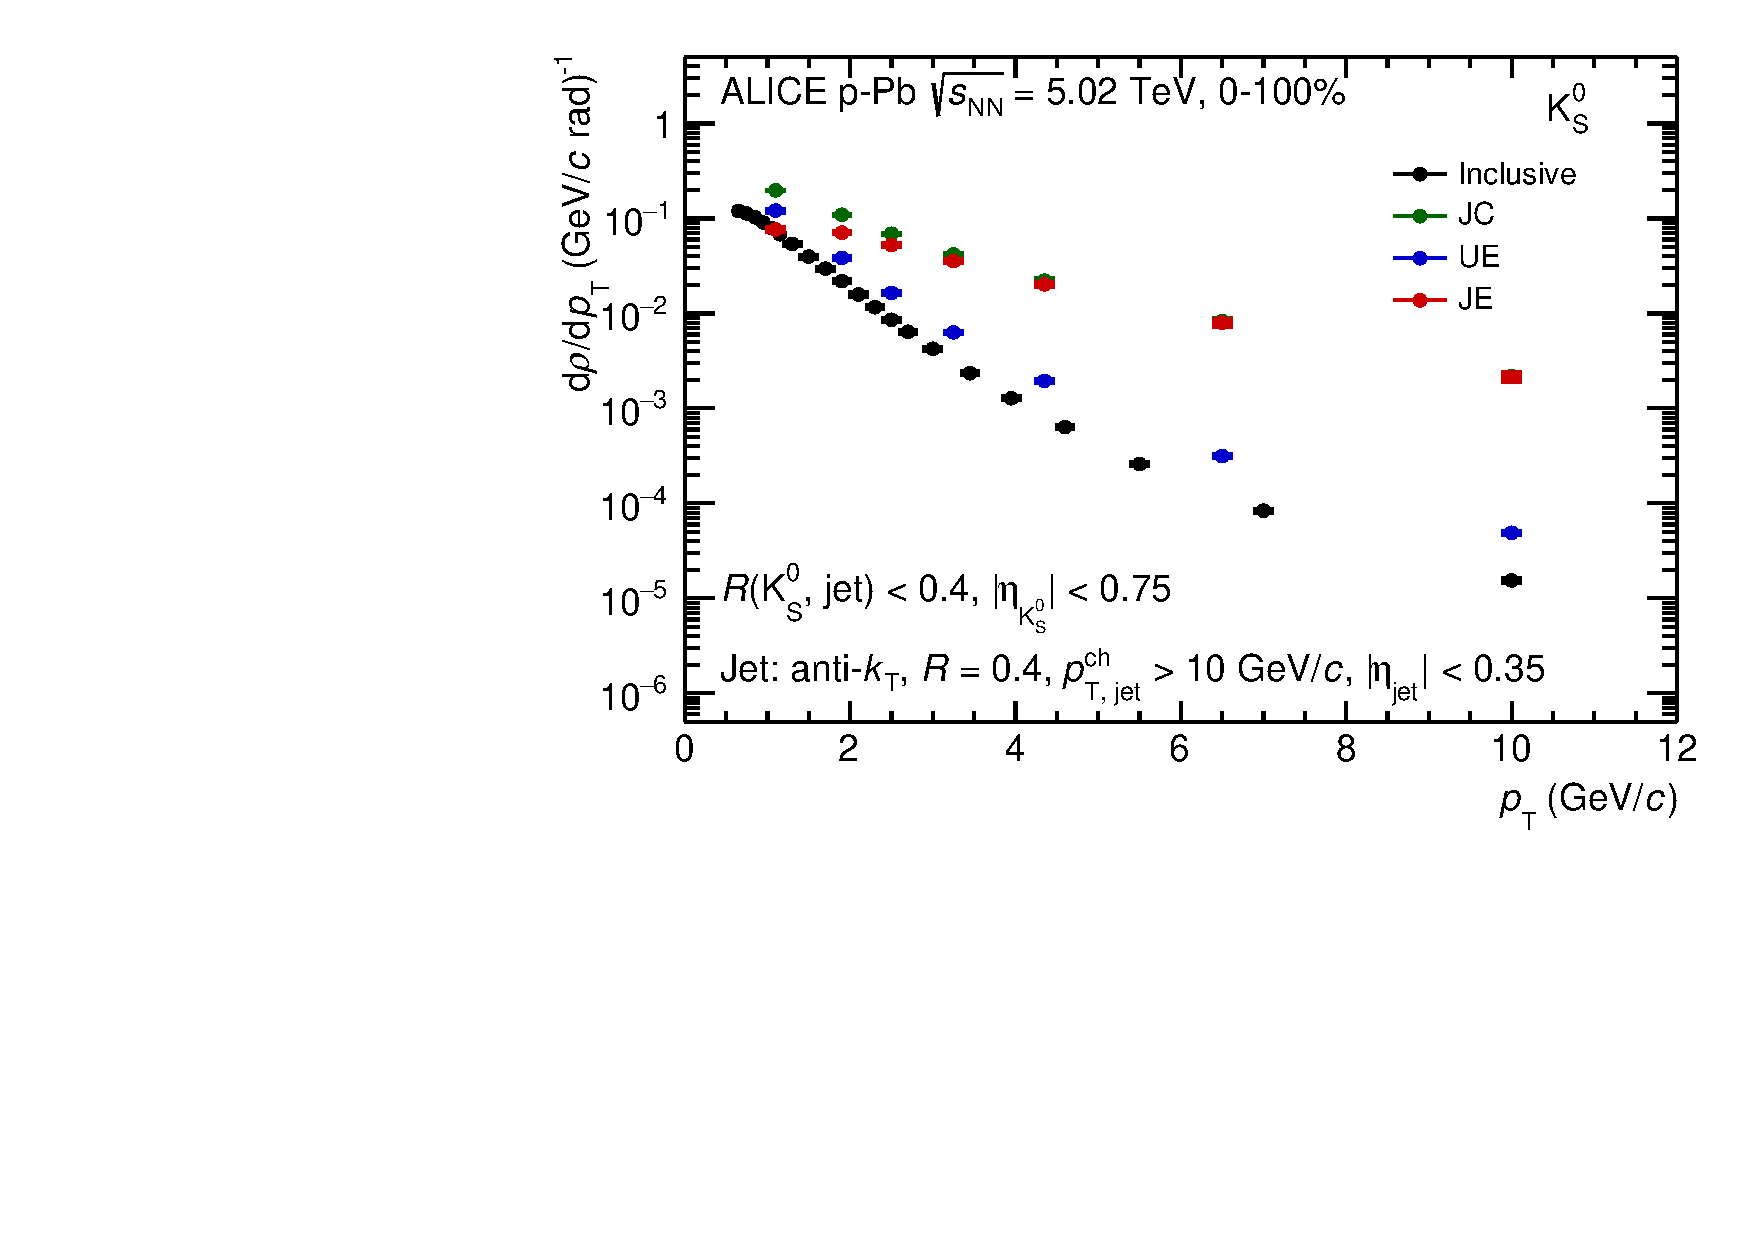
\includegraphics[width=.4\textwidth]{cf05_1}
%DIFDELCMD < 		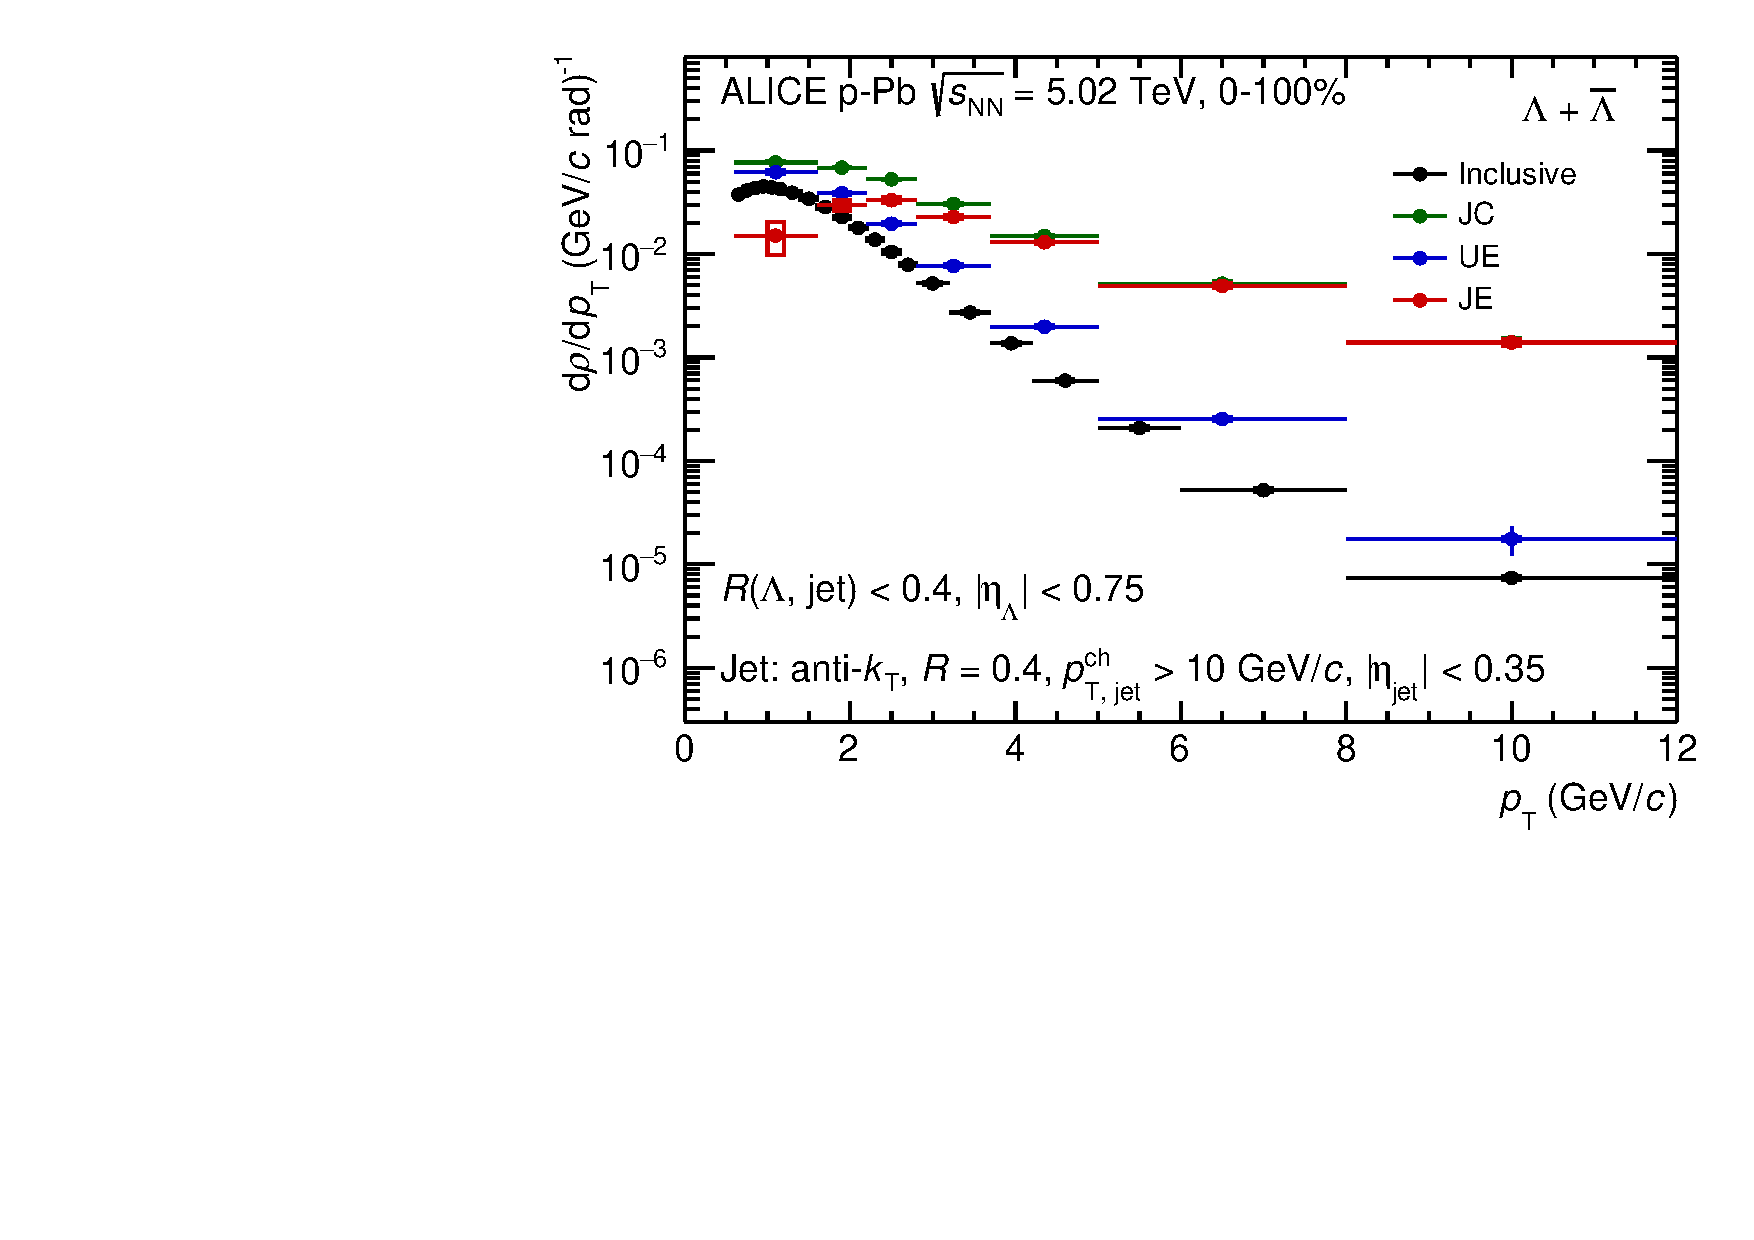
\includegraphics[width=.4\textwidth]{cf05_2}
%DIFDELCMD < 		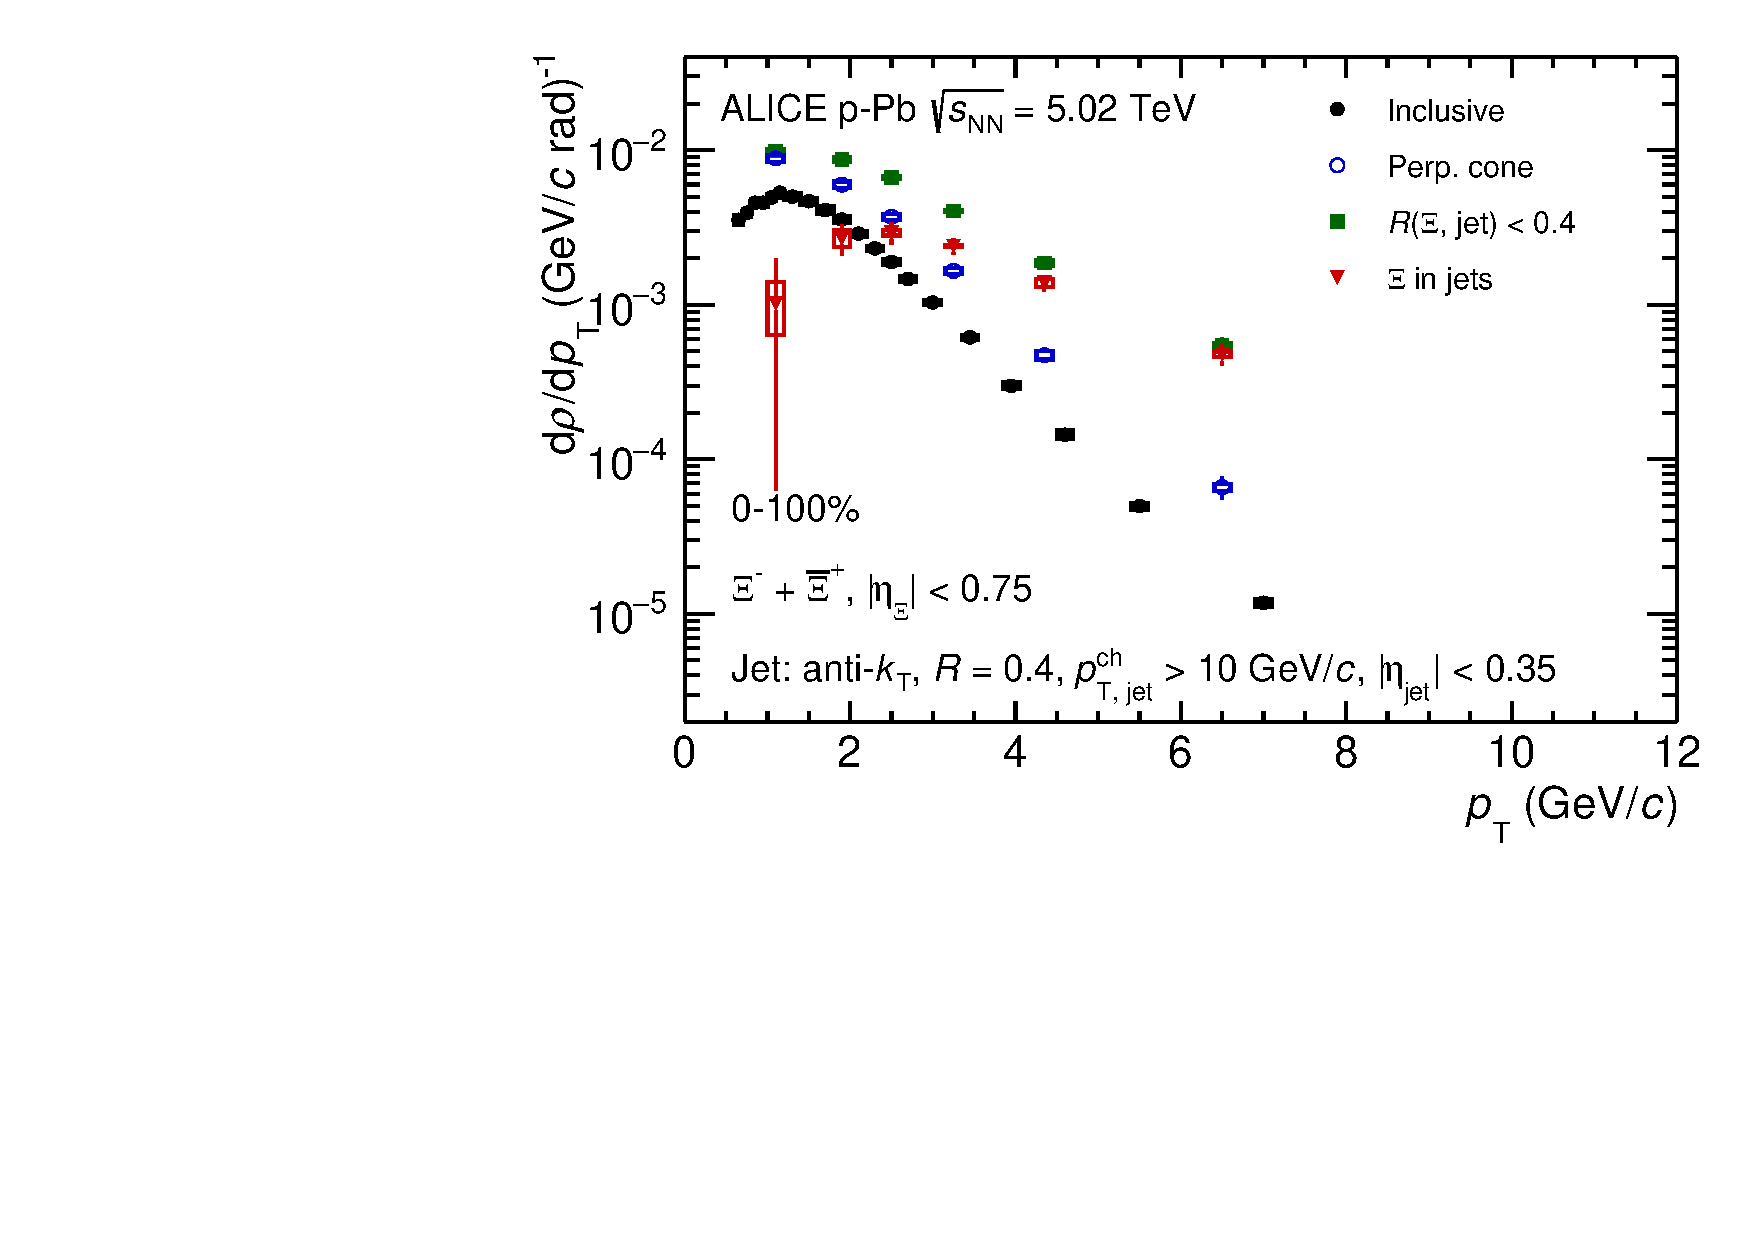
\includegraphics[width=.4\textwidth]{cf05_3}
%DIFDELCMD < 		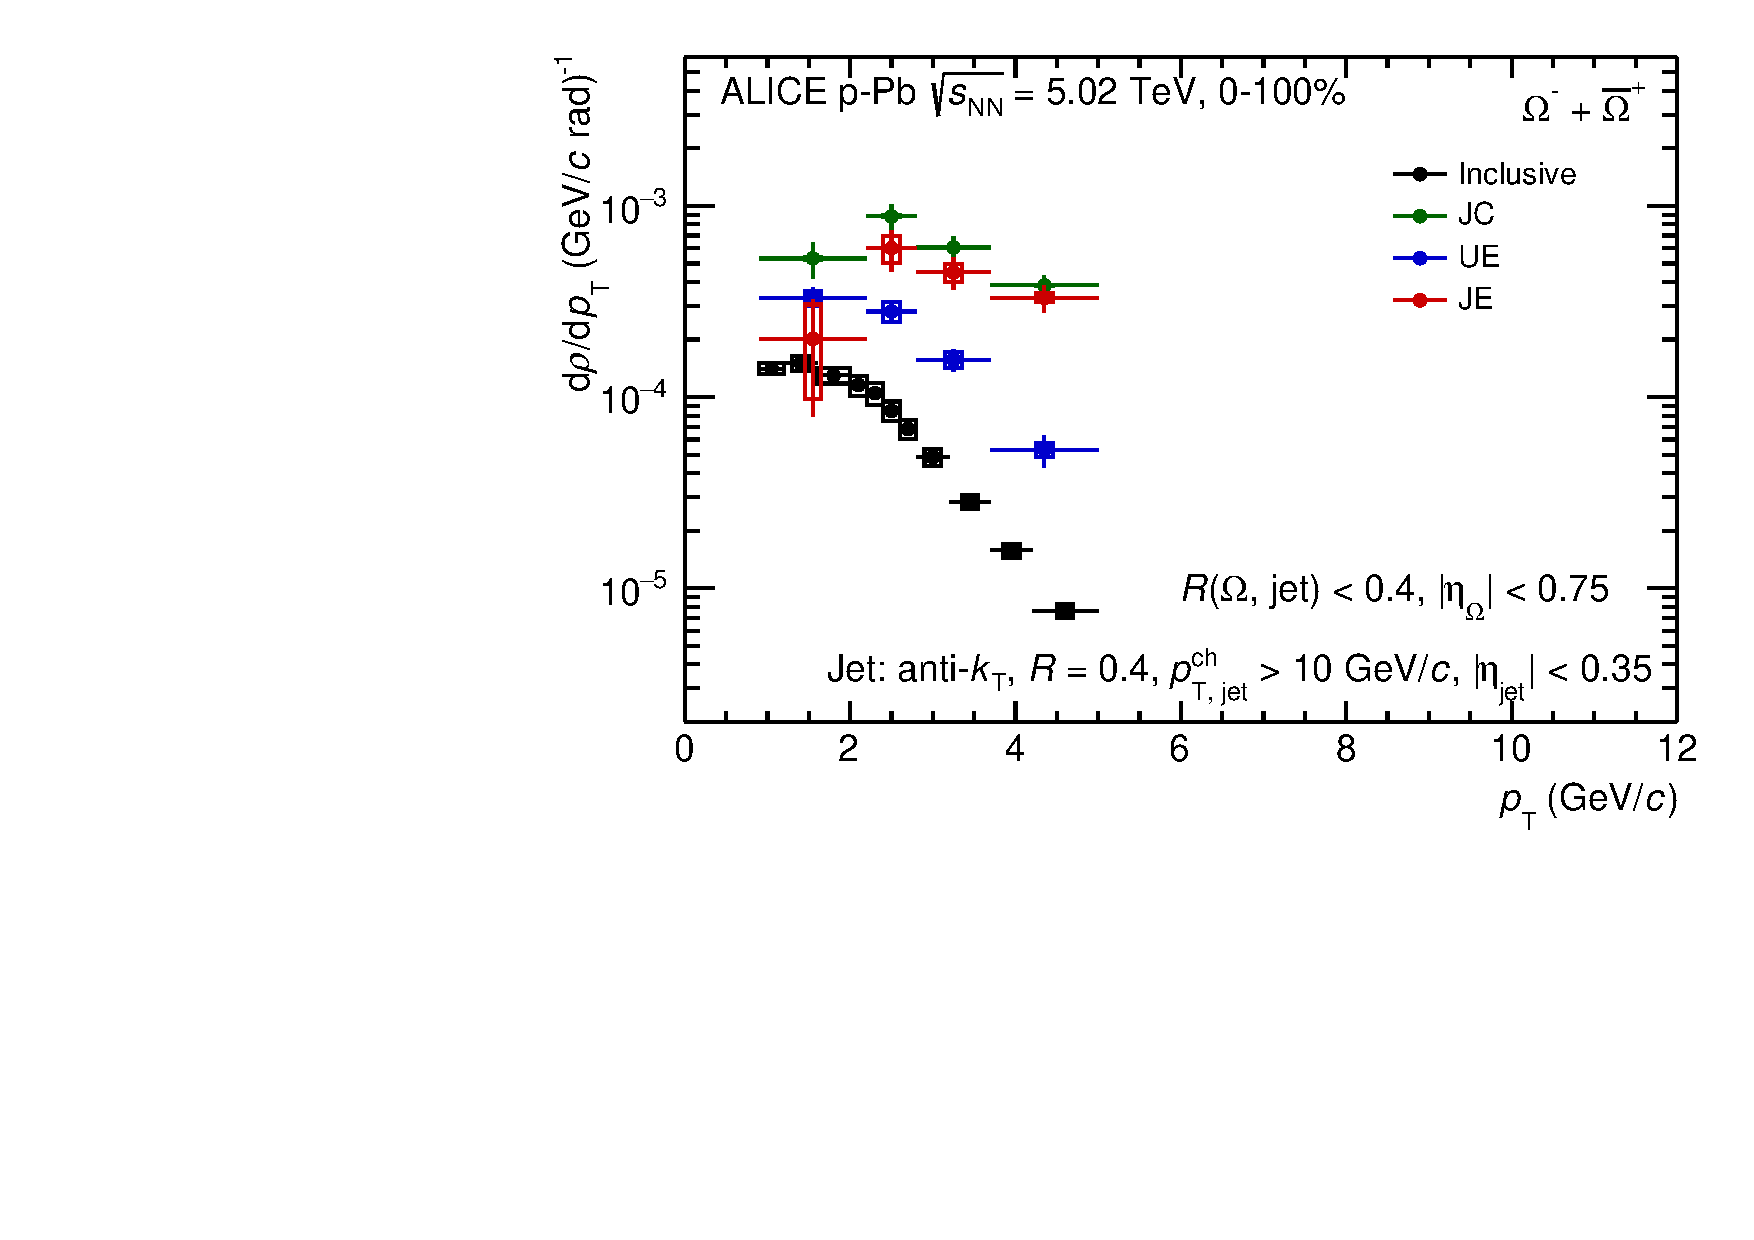
\includegraphics[width=.4\textwidth]{cf05_4}
%DIFDELCMD < 	\end{center}
%DIFDELCMD < 	%%%
%DIFDELCMD < \caption{%
{%DIFAUXCMD
\DIFdelFL{$\pT$-differential density of $\kzero$, $\lmb + \almb$, $\X + \Ix$ and $\Om + \Mo$ in 0-100\% in }%DIFDELCMD < \pPb %%%
\DIFdelFL{at }%DIFDELCMD < \fivenn%%%
\DIFdelFL{. In those plots, the black point depicts particles witch from minimum bias events, the green point depicts particles which from the jet cones, the blue point depicts particles within perpendicular cone of jet which associated with the underlying event and the red point depicts the particle from the jet fragmentation.}}
	%DIFAUXCMD
%DIFDELCMD < \label{fig:pPbSpect}
%DIFDELCMD < \end{figure}
%DIFDELCMD < 

%DIFDELCMD < %%%
\DIFdelend \DIFaddbegin \DIFadd{In the previous studies of ALICE experiment~\mbox{%DIFAUXCMD
\cite{ALICE:2015mpp, ALICE:2016dei, ALICE:2013wgn}}\hspace{0pt}%DIFAUXCMD
, the stronger multiplicity dependence of the inclusive $\pT$-differential spectra shapes of heavier particles is observed.
It also a important evidence for the baryon-to-meson ratio enhancement at intermediate-$\pT$.
}\DIFaddend The $\pT$\DIFaddbegin \DIFadd{-differential densities }\DIFaddend distributions of $\kzero$, $\lmb + \almb$\DIFaddbegin \DIFadd{, $\X + \Ix$ and $\Om + \Mo$ particles within jet are shown in Fig.~\ref{fig:pPbSpectwCent} for different charged-particle multiplicity bins.
The bottom panels depict the ratio to the minimum bias (0-100\%) $\pT$ distribution.
For the $\Om + \Mo$ in jet density, only the minimum bias distribution is shown.
These spectra are compared to the particles in charged-particle jets with PYTHIA 8 simulation with Monash tune.
The PYTHIA 8 can describe the $\kzero$ }\DIFaddend and \DIFaddbegin \DIFadd{$\lmb + \almb$ well, but not for the }\DIFaddend $\X + \Ix$ \DIFdelbegin \DIFdel{for the event classes defined in Tab.
~\ref{tab:multi} are show in }\DIFdelend \DIFaddbegin \DIFadd{and $\Om + \Mo$.
In }\DIFaddend Fig.~\ref{fig:pPbSpectwCent}\DIFdelbegin \DIFdel{. The inclusive distributions become harder with increasing }\DIFdelend \DIFaddbegin \DIFadd{, the $\kzero$, $\lmb + \almb$ and $\X + \Ix$  particle $\pT$ spectra do not show any dependent on the }\DIFaddend charged-particle multiplicity \DIFdelbegin \DIFdel{. Particles in JE, which generated by jet fragmentation , are systematically independent with centrality classes.
}\DIFdelend \DIFaddbegin \DIFadd{which observed in that of inclusive particles~\mbox{%DIFAUXCMD
\cite{ALICE:2015mpp, ALICE:2016dei, ALICE:2013wgn}}\hspace{0pt}%DIFAUXCMD
. 
Then the particle associated with jet fragmentation process may not contribute on the baryon-to-meson ratio enhancement in high multiplicity INEL events with respect to that in lower multiplicity events in small collision systems.
}

\DIFaddend \begin{figure}[!ht]
	\begin{center}
		\DIFdelbeginFL %DIFDELCMD < 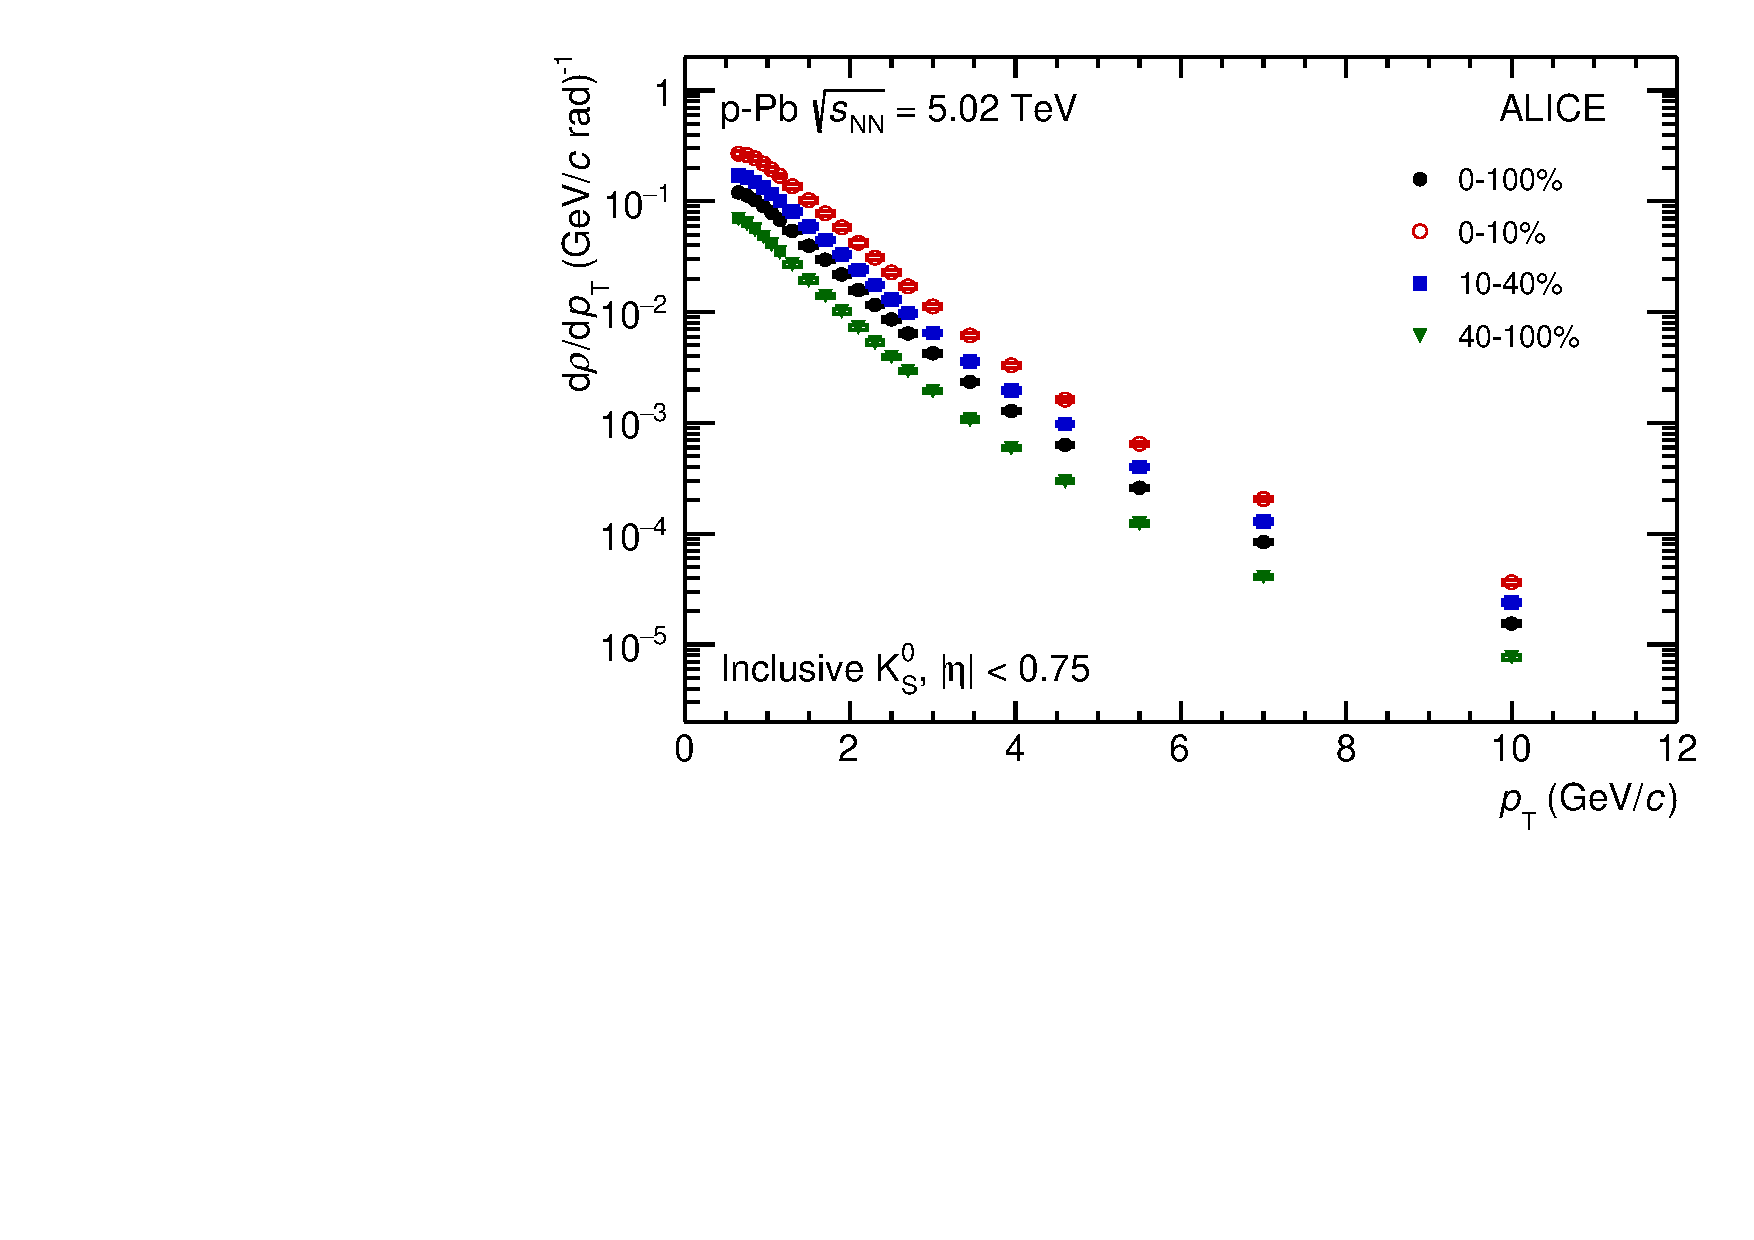
\includegraphics[width=.3\textwidth]{cf06_1}
%DIFDELCMD < 		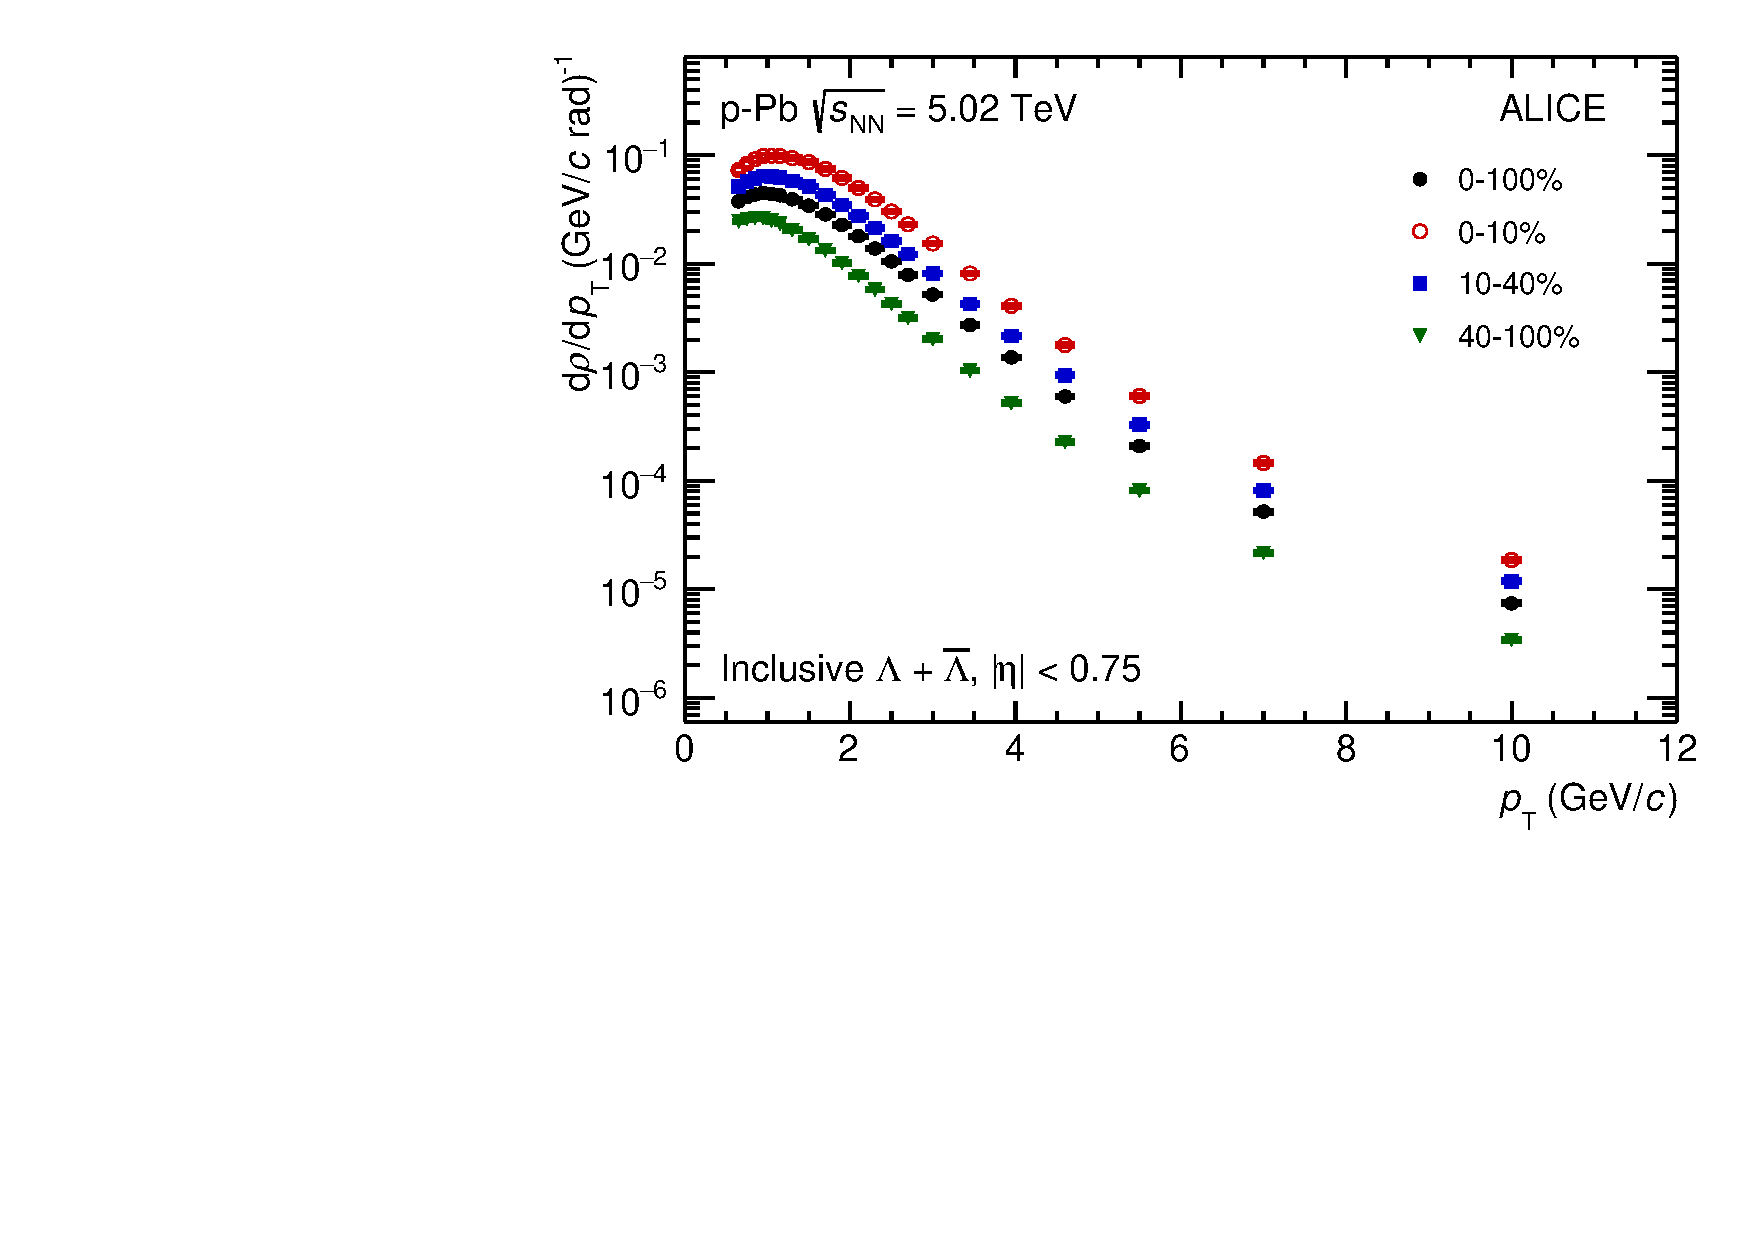
\includegraphics[width=.3\textwidth]{cf06_2}
%DIFDELCMD < 		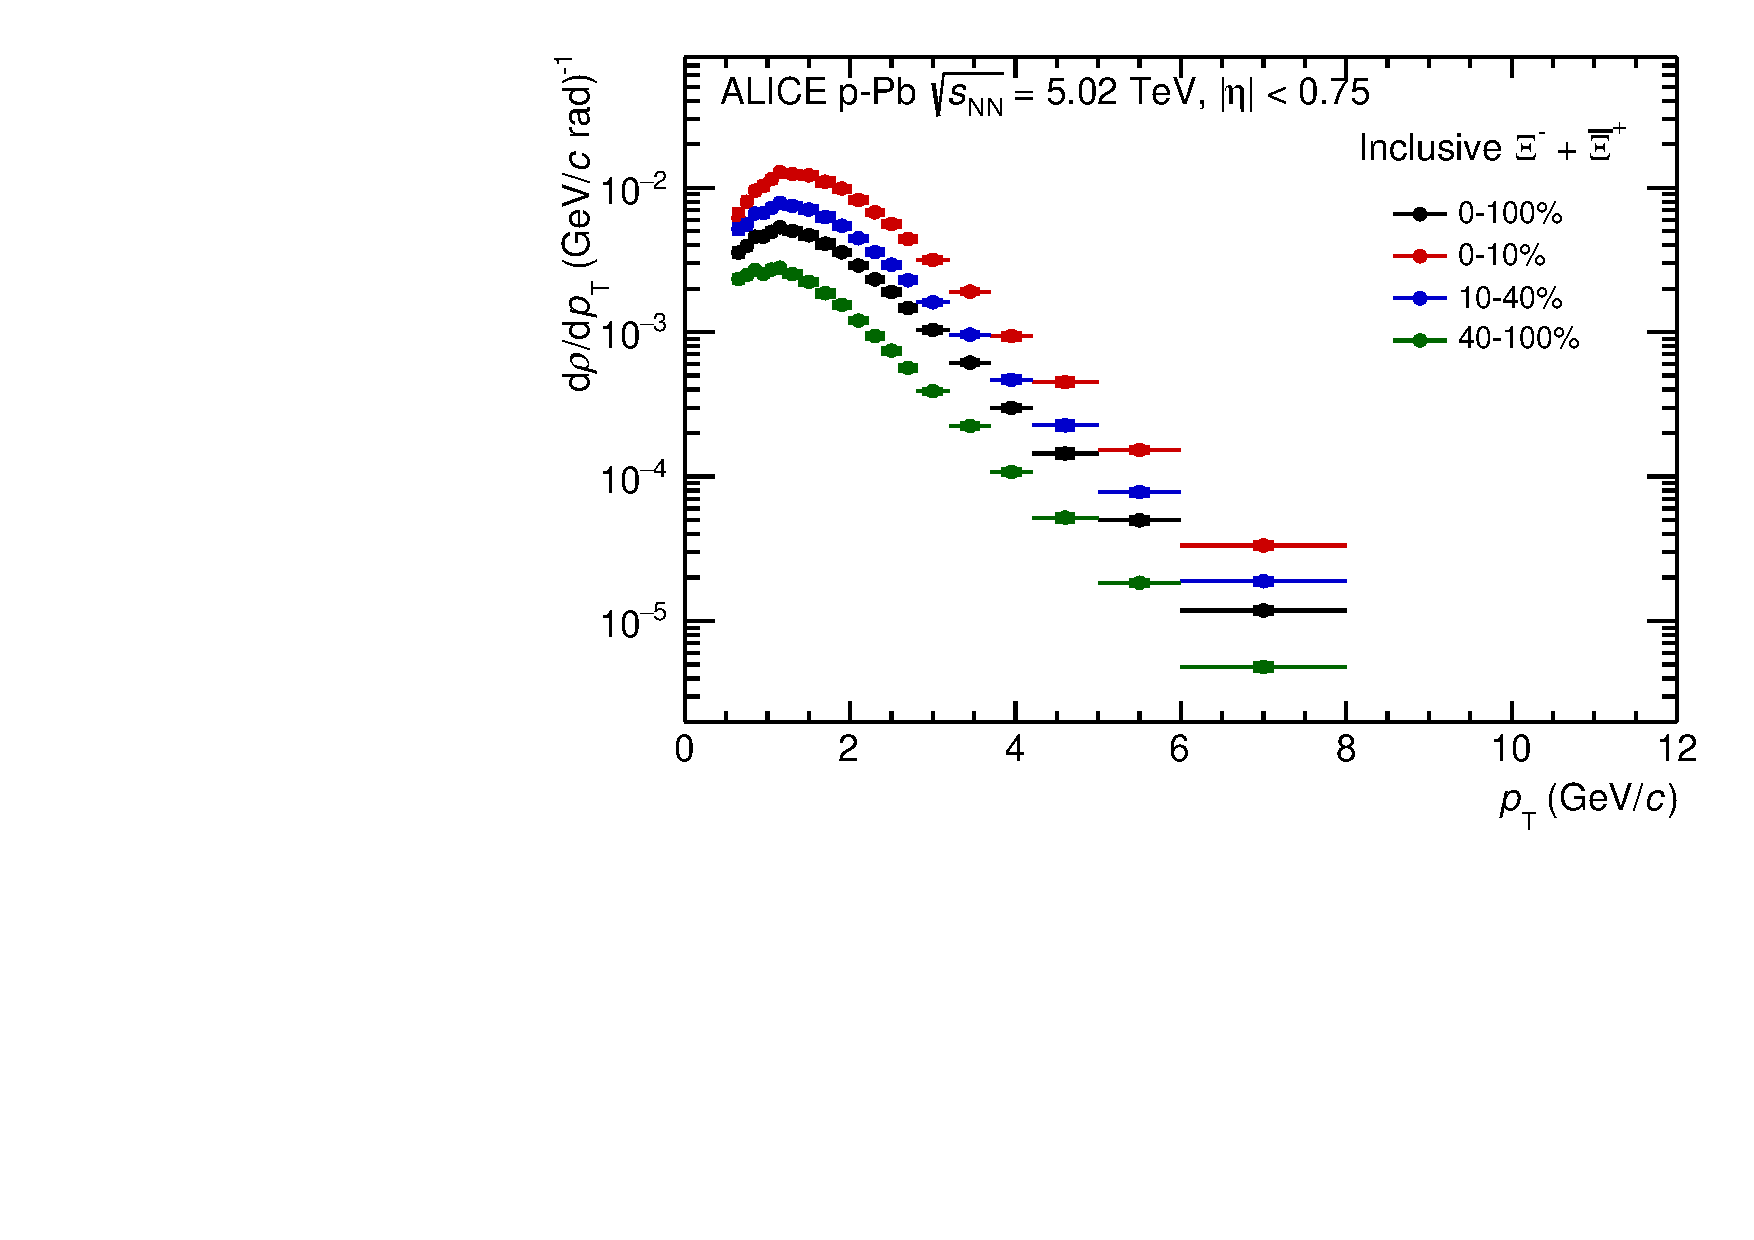
\includegraphics[width=.3\textwidth]{cf06_3}
%DIFDELCMD < 		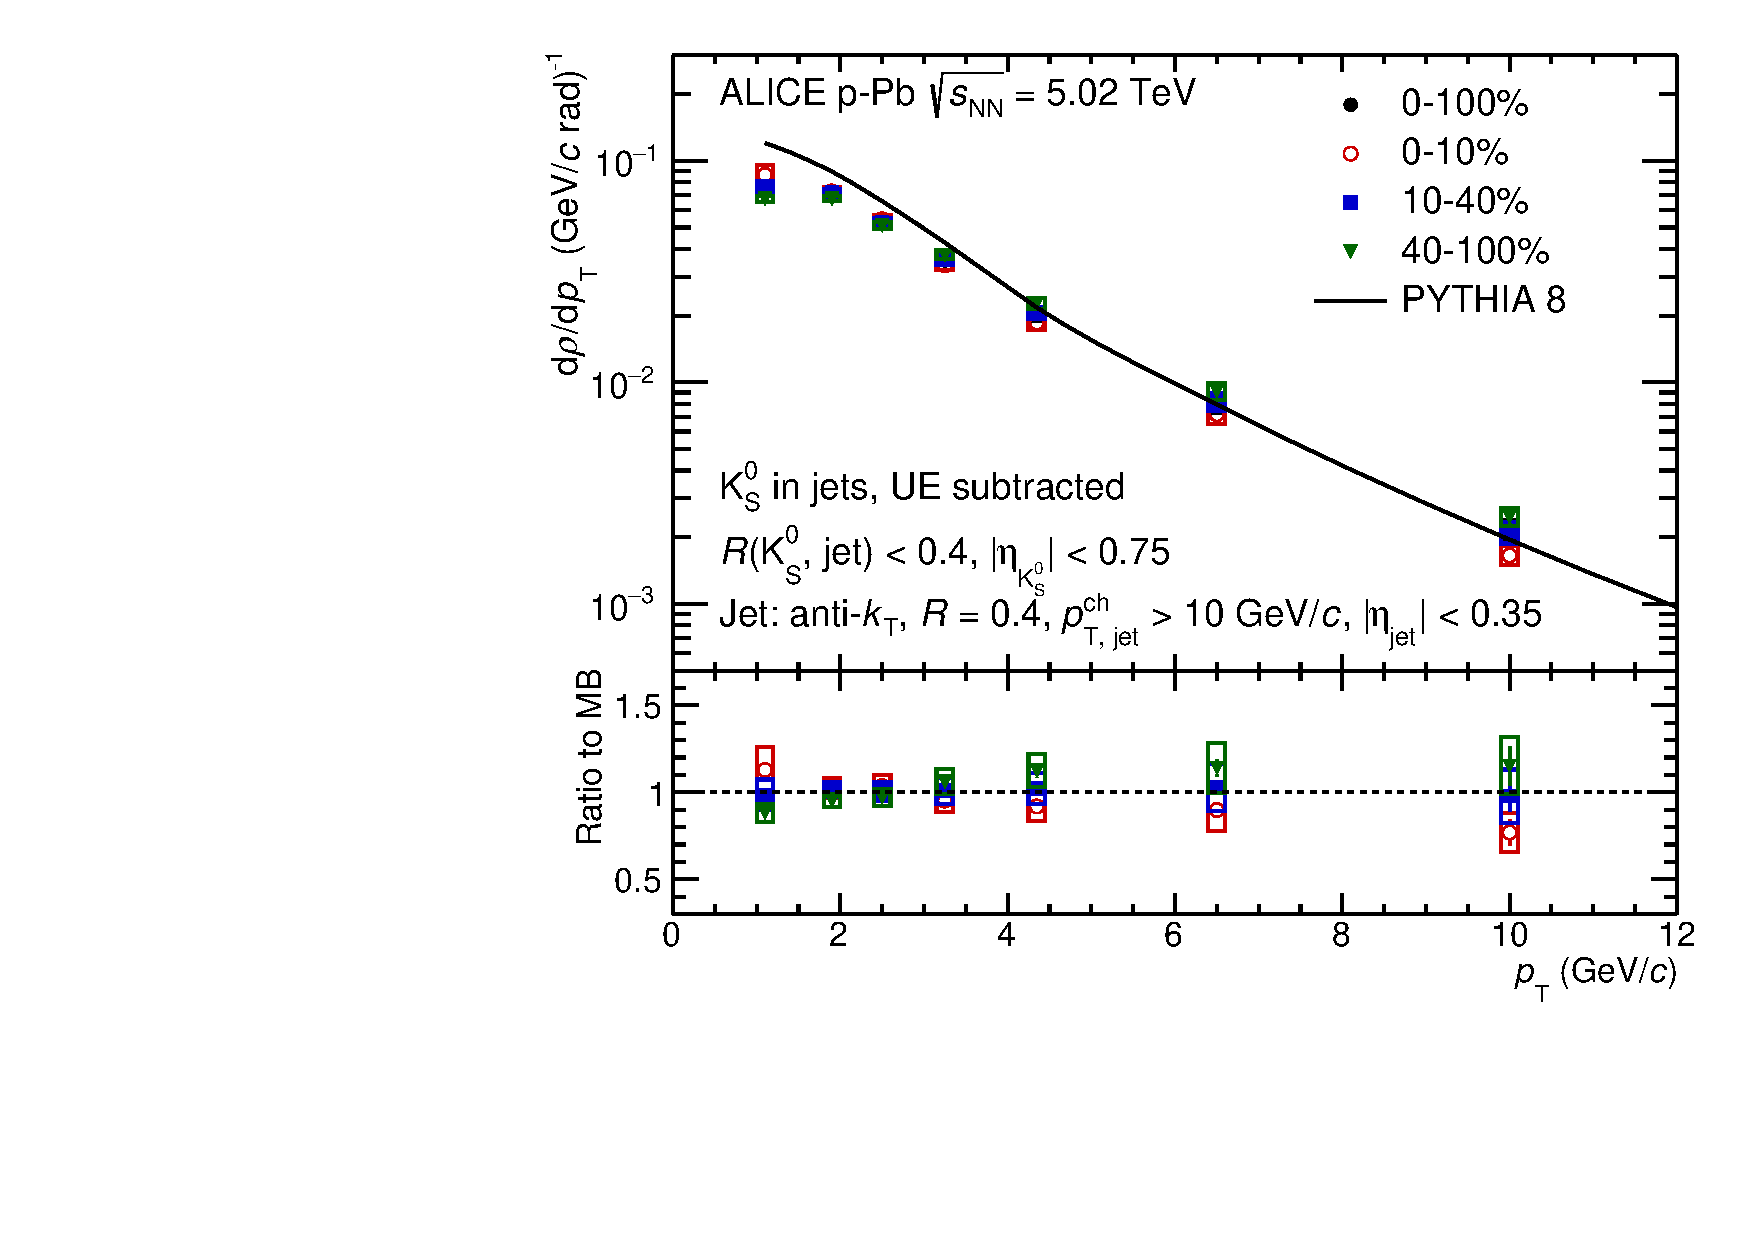
\includegraphics[width=.3\textwidth]{cf06_4}
%DIFDELCMD < 		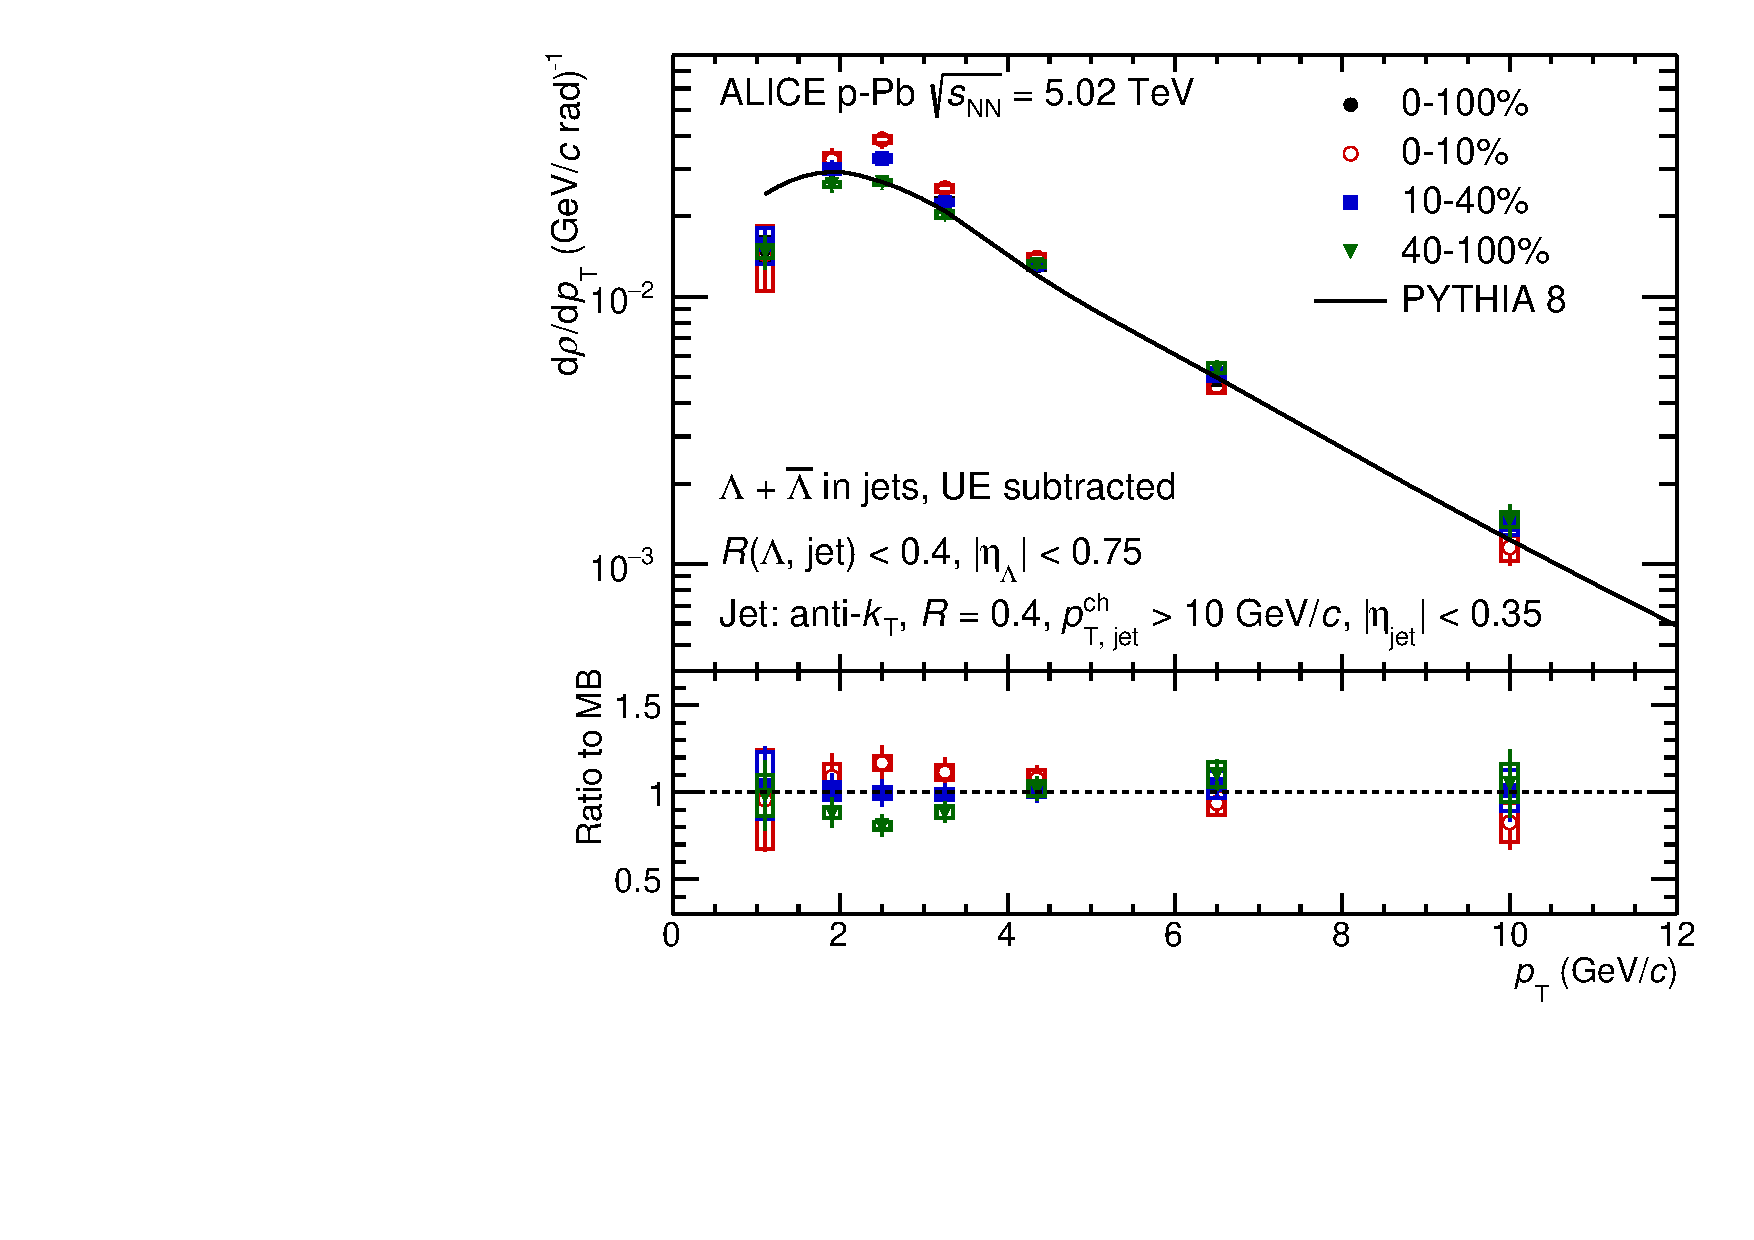
\includegraphics[width=.3\textwidth]{cf06_5}
%DIFDELCMD < 		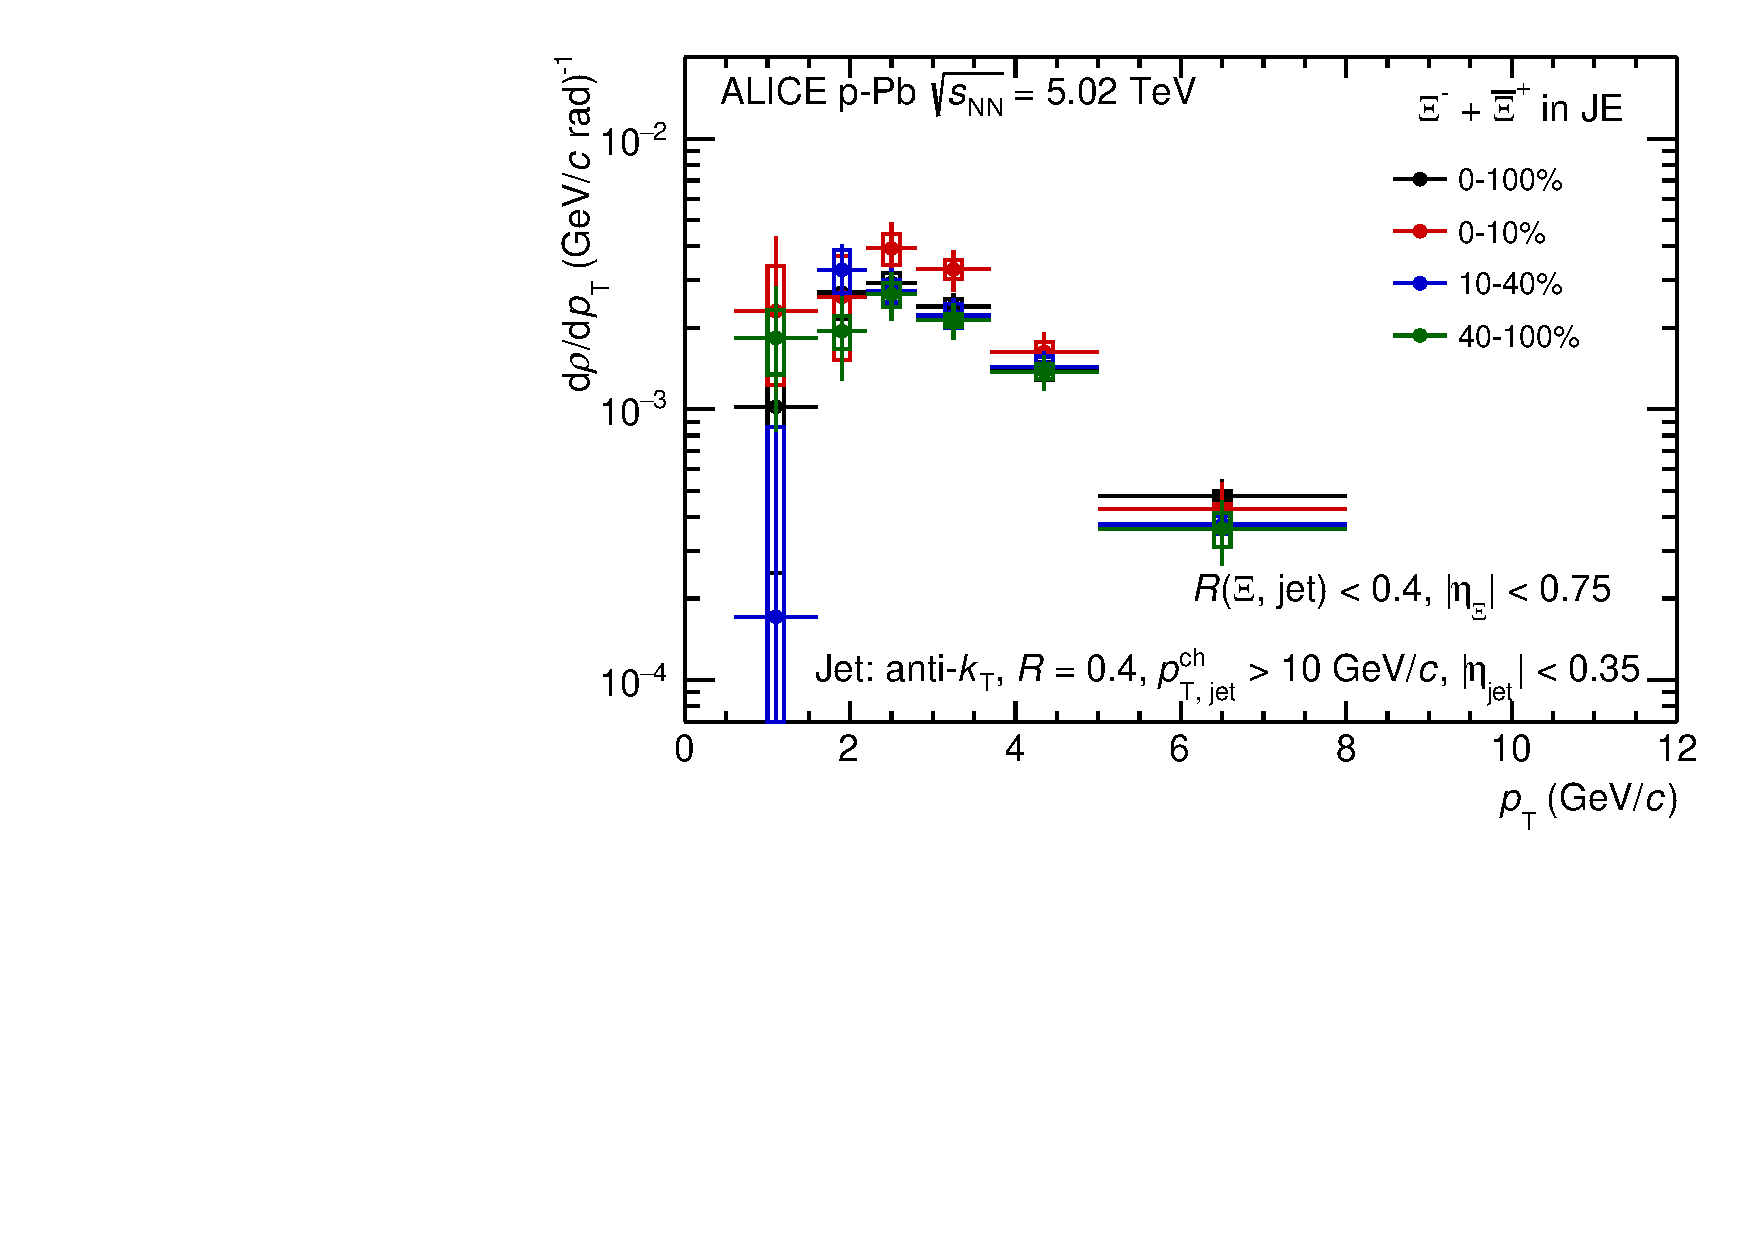
\includegraphics[width=.3\textwidth]{cf06_6}
%DIFDELCMD < 	%%%
\DIFdelendFL %DIF > 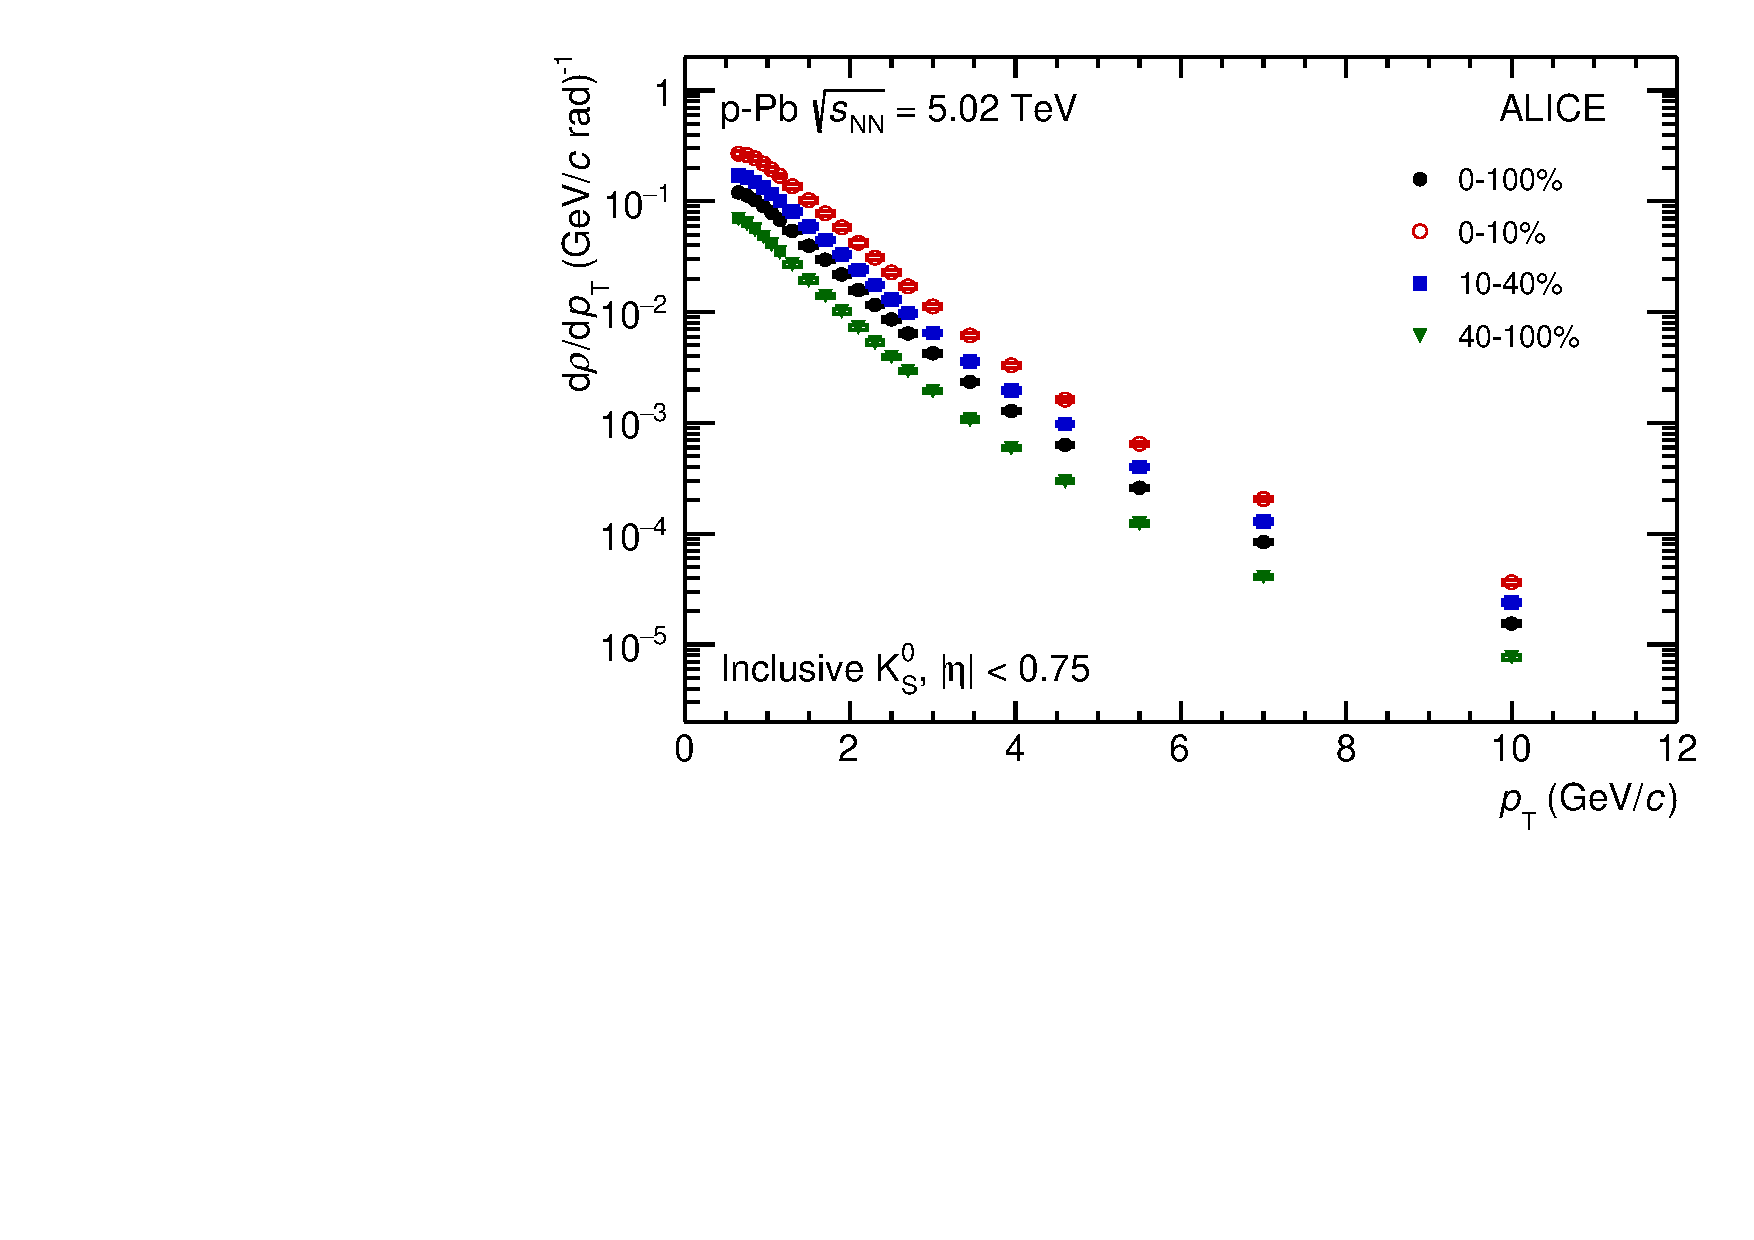
\includegraphics[width=.32\textwidth]{cf06_1}
		%DIF > 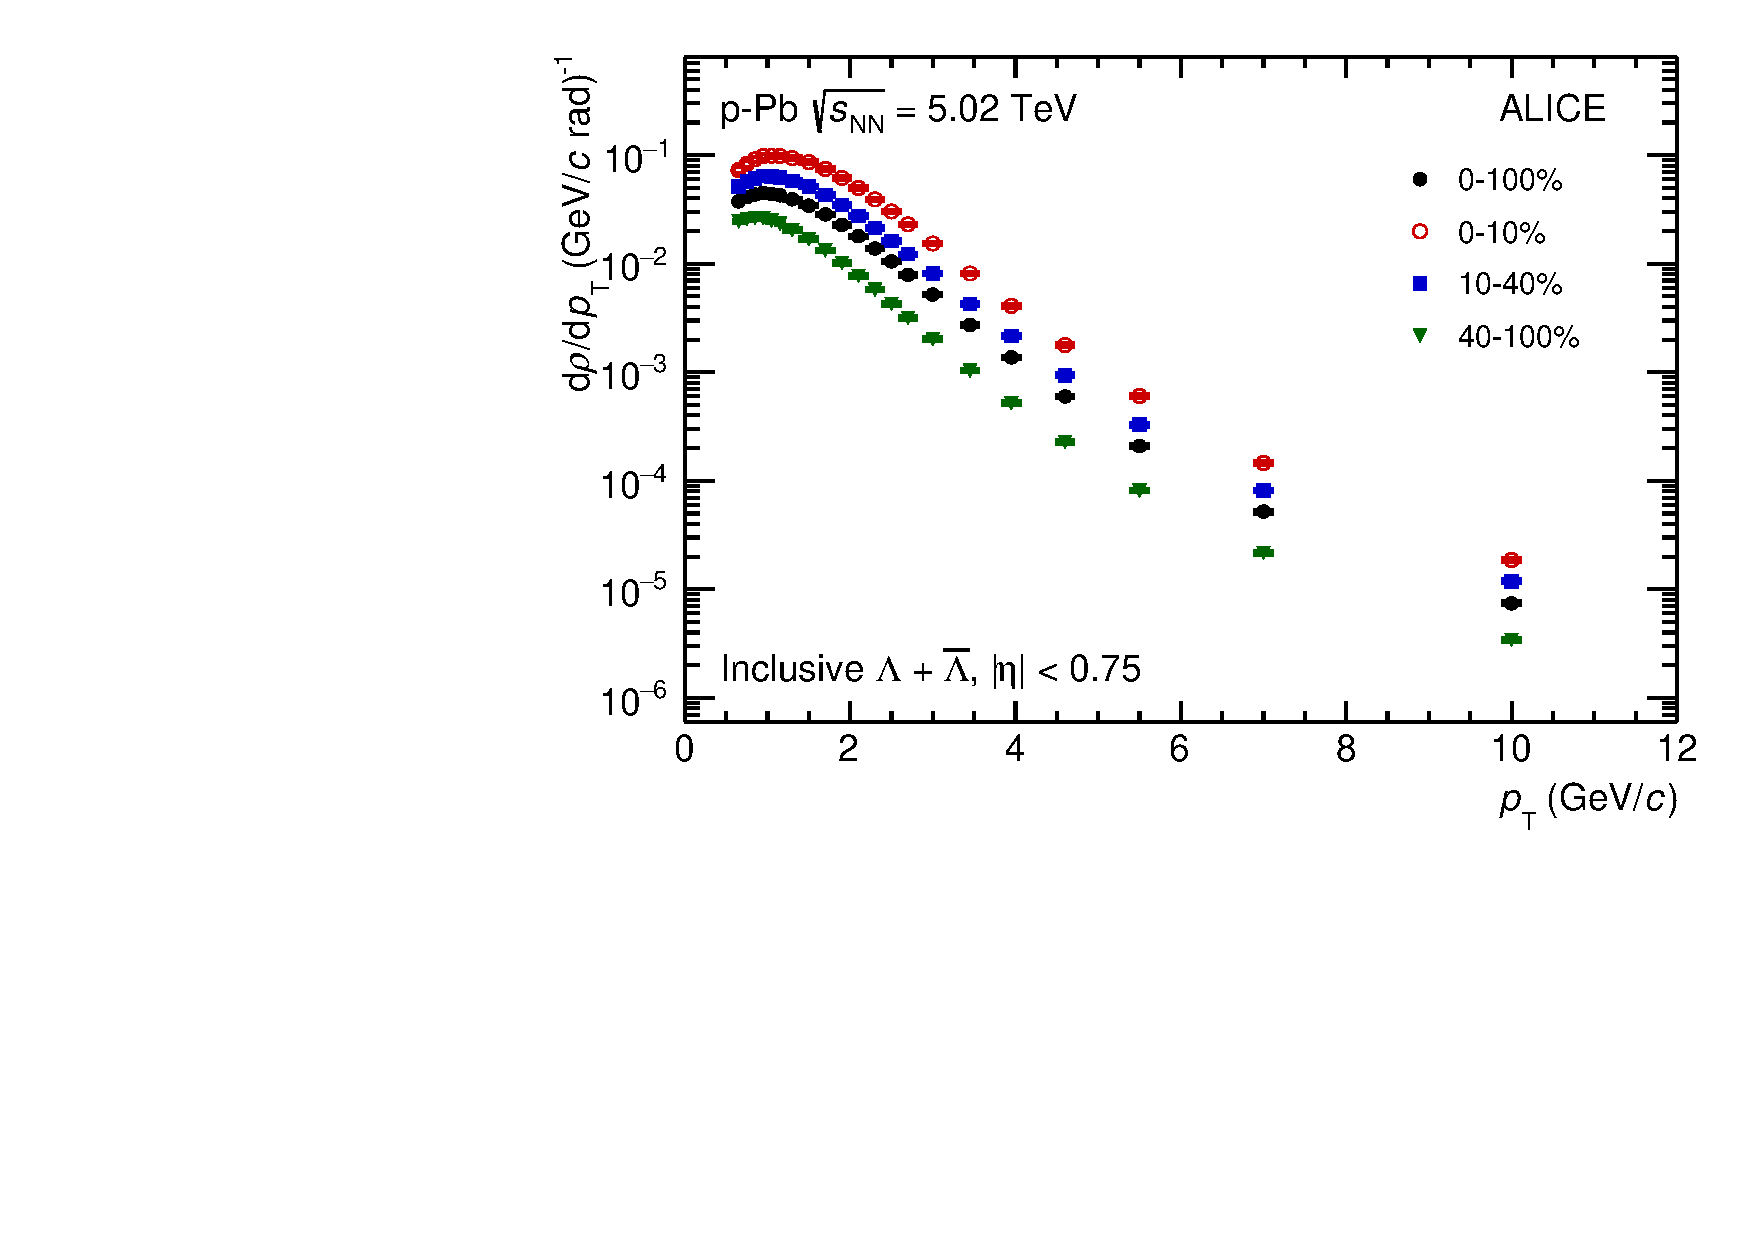
\includegraphics[width=.32\textwidth]{cf06_2}
		%DIF > 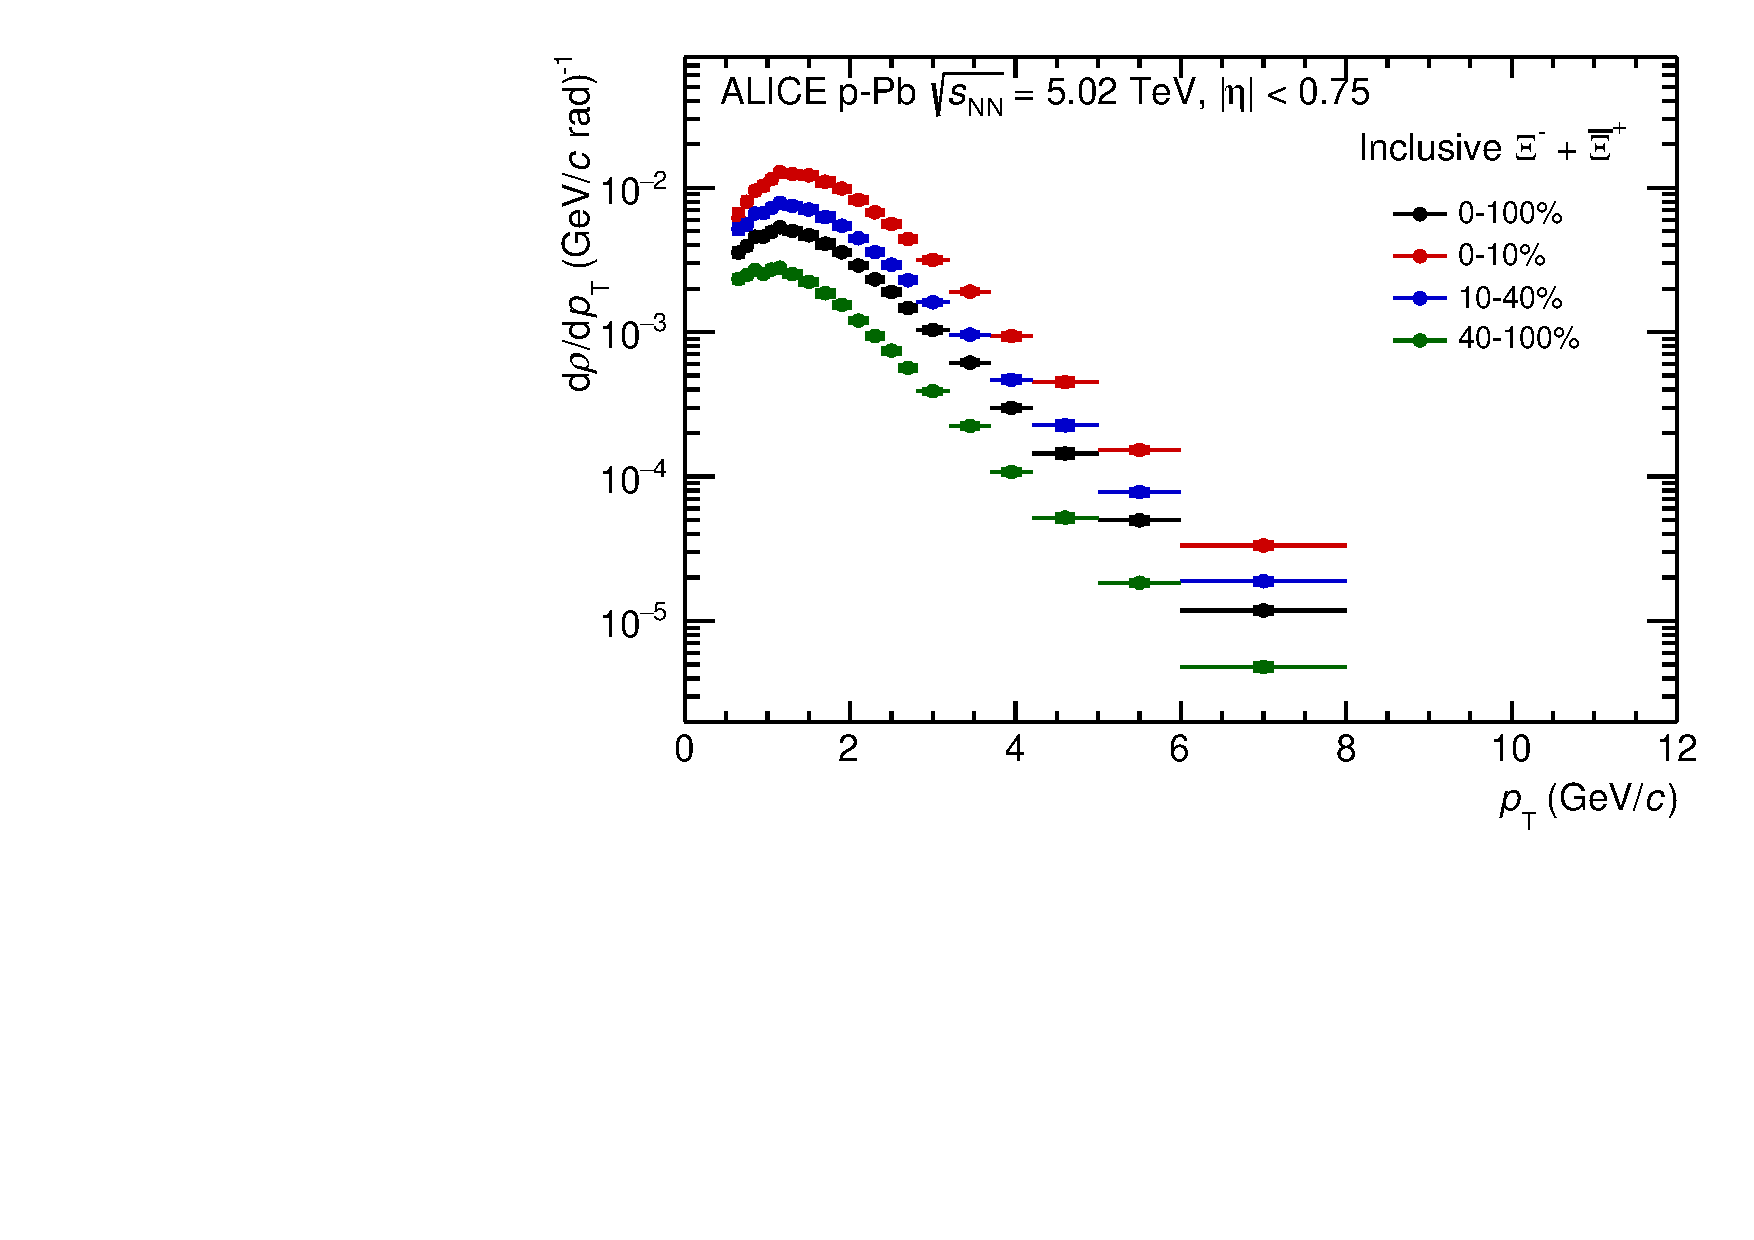
\includegraphics[width=.32\textwidth]{cf06_3}
		\DIFaddbeginFL 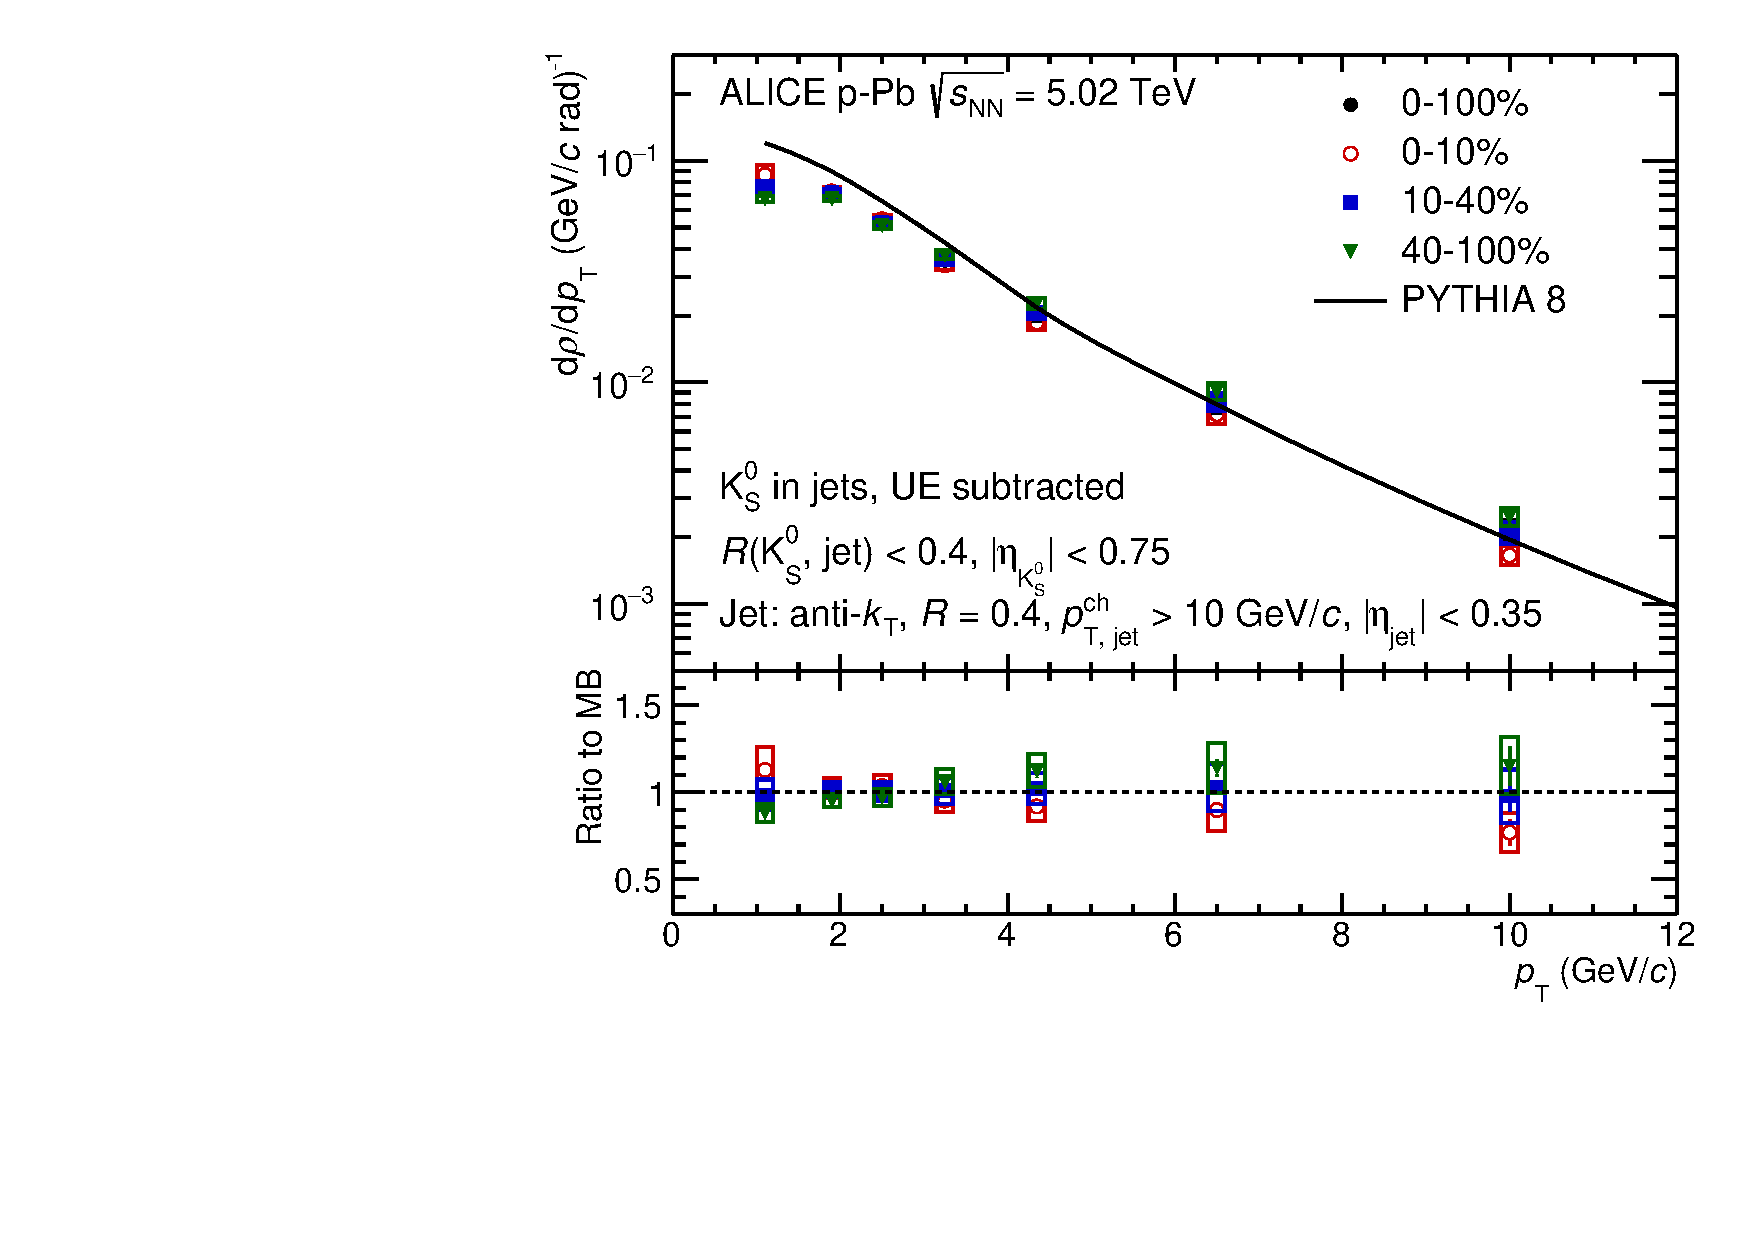
\includegraphics[width=.49\textwidth]{cf06_4}
		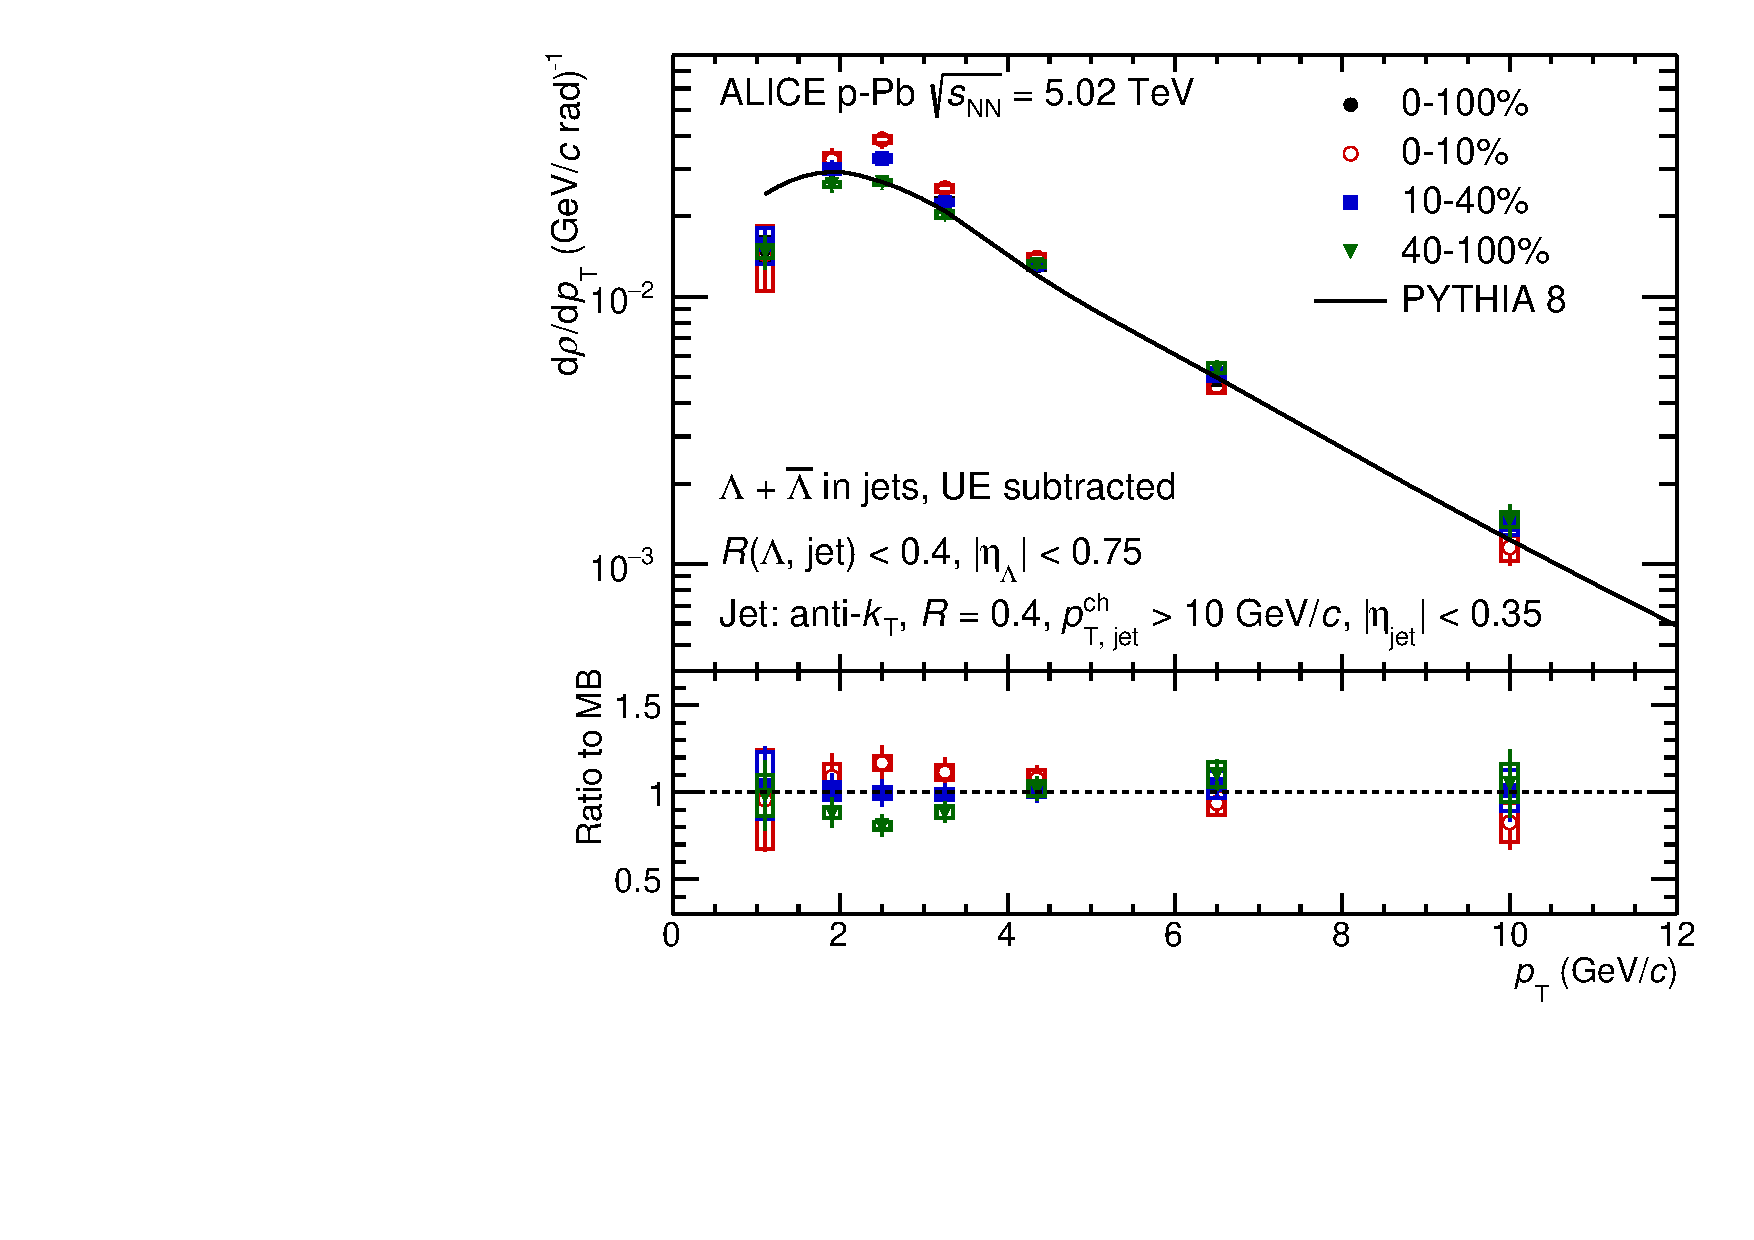
\includegraphics[width=.49\textwidth]{cf06_5}
		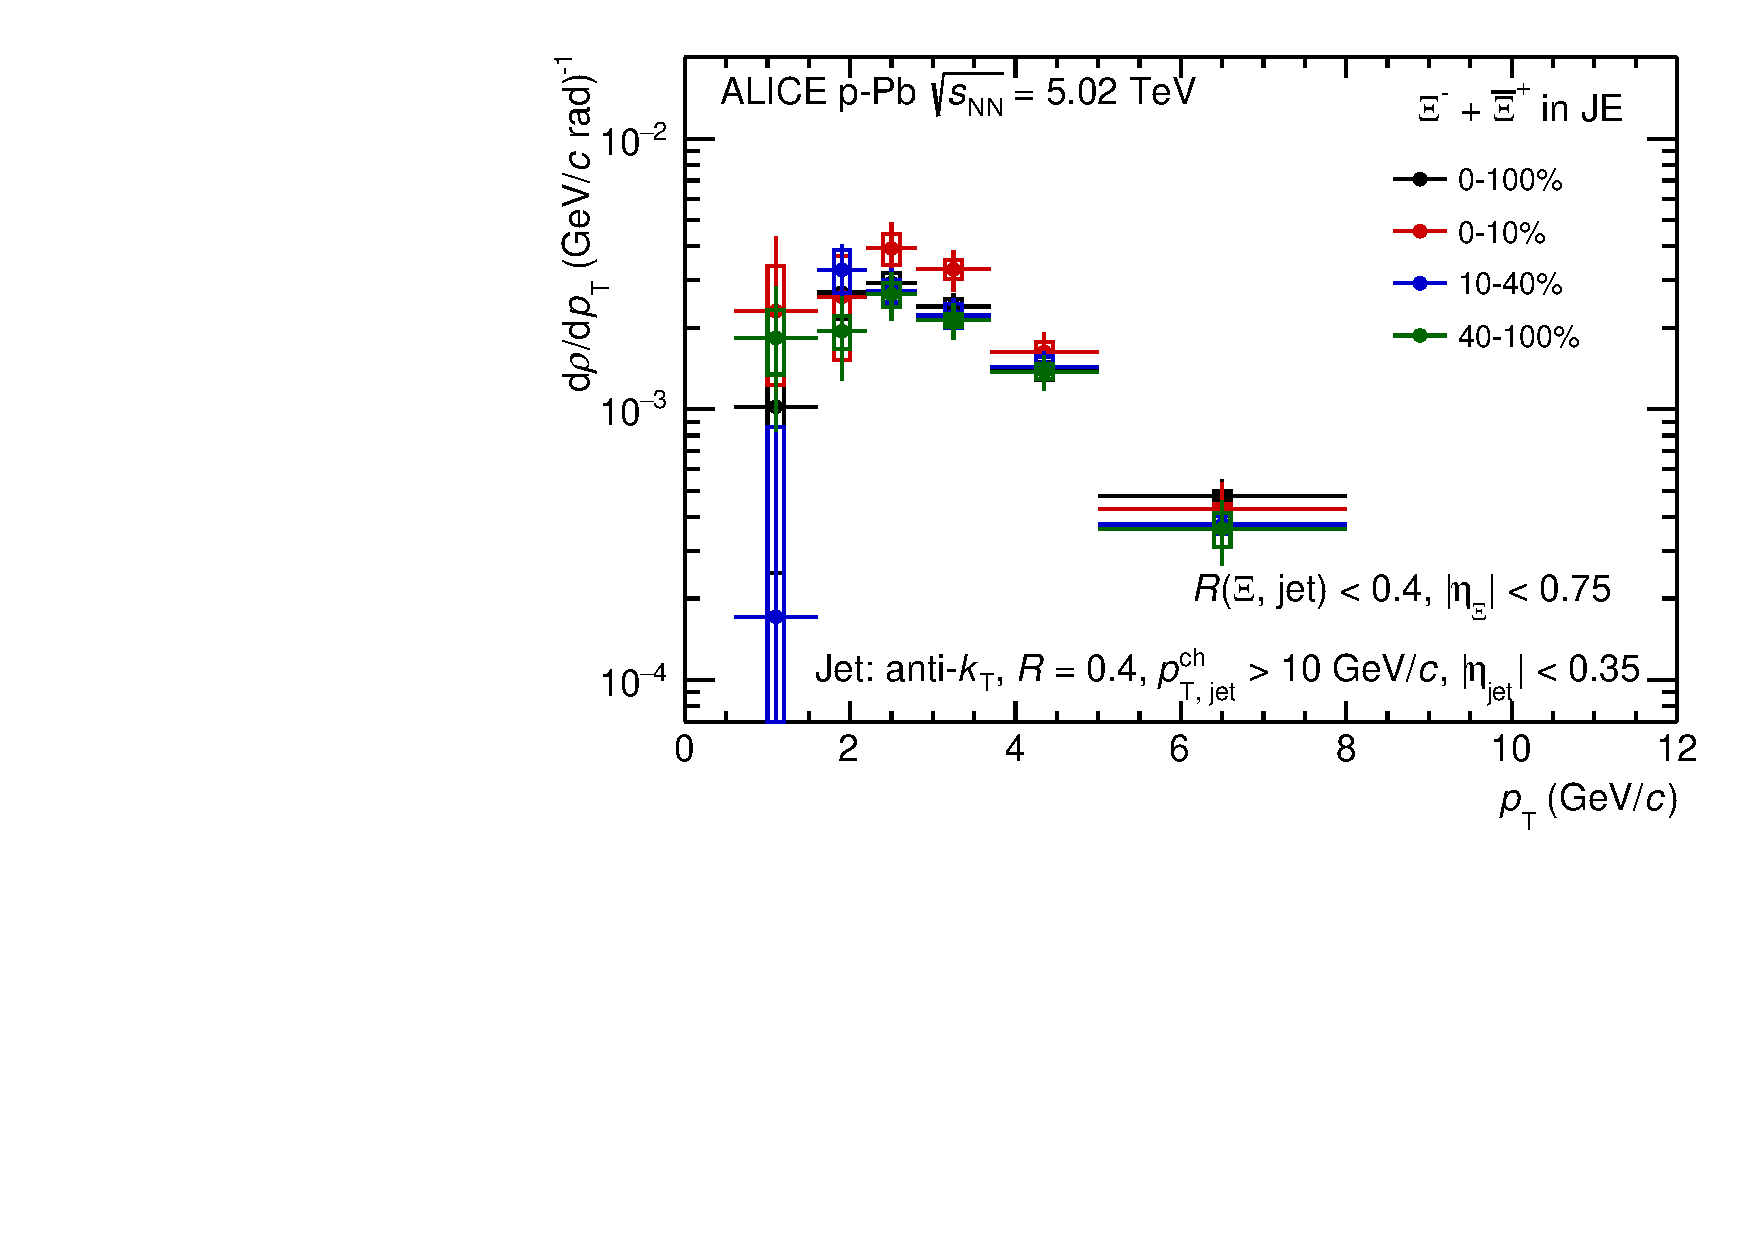
\includegraphics[width=.49\textwidth]{cf06_6}
		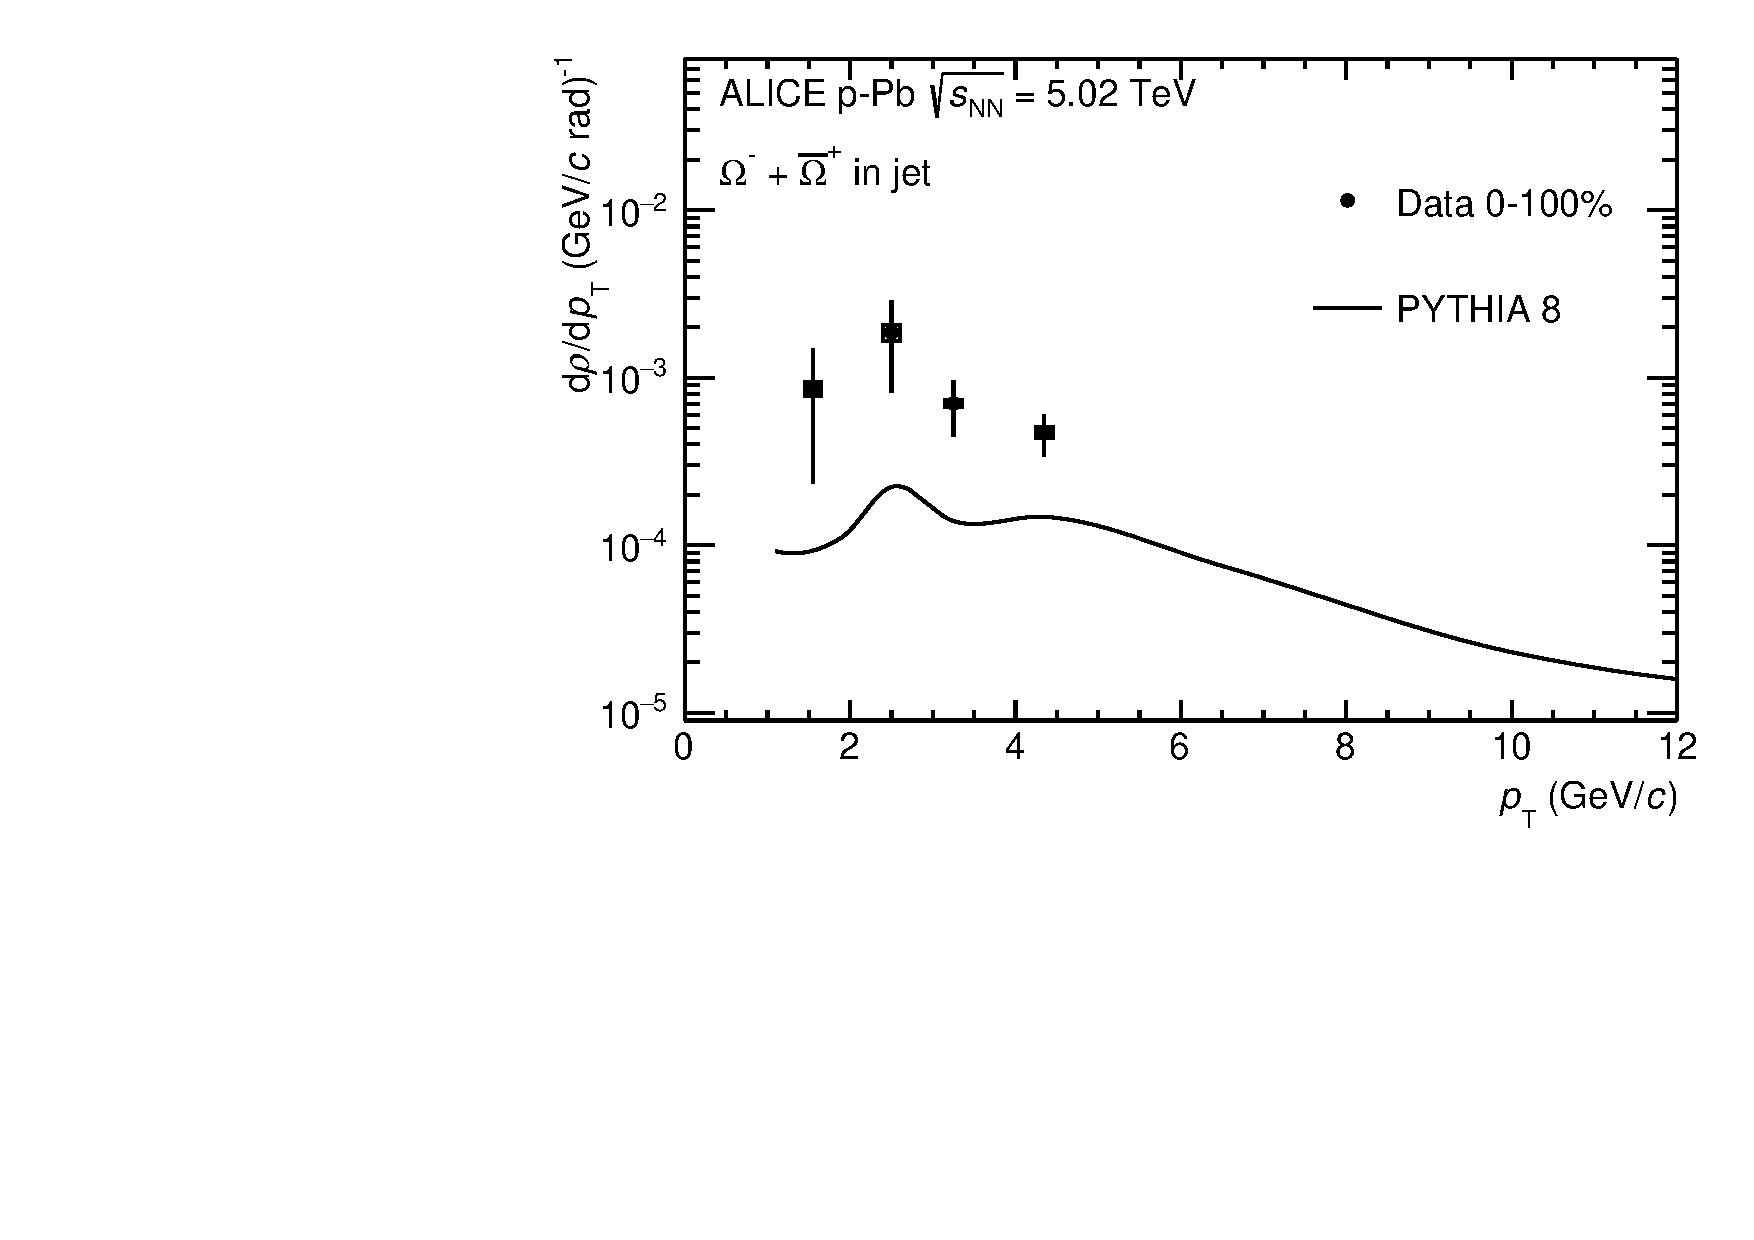
\includegraphics[width=.49\textwidth]{cf06_7}
	\DIFaddendFL \end{center}
	\caption{$\pT$-differential density of $\kzero$, $\lmb + \almb$\DIFdelbeginFL \DIFdelFL{and }\DIFdelendFL \DIFaddbeginFL \DIFaddFL{, }\DIFaddendFL $\X + \Ix$ \DIFaddbeginFL \DIFaddFL{and $\Om + \Mo$ (0-100\% only) particles within jets }\DIFaddendFL in different V0A event \DIFdelbeginFL \DIFdelFL{centrality }\DIFdelendFL \DIFaddbeginFL \DIFaddFL{multiplicity }\DIFaddendFL classes in \pPb \DIFaddbeginFL \DIFaddFL{collisions }\DIFaddendFL at \fivenn. \DIFdelbeginFL \DIFdelFL{Top panels show the inclusive particle and bottom panels show particles generated by jet fragmentation. }\DIFdelendFL The different centrality classes are depicted with different color. \DIFaddbeginFL \DIFaddFL{In the bottom panels ratios of multiplicity dependent spectra to minimum bias are shown. The systematic uncertainties on the ratios are obtained by considering only contributions uncorrelated across multiplicity.
	The dashed curves represent PYTHIA 8 simulations to the measured spectra.
	}\DIFaddendFL }
	\label{fig:pPbSpectwCent}
\end{figure}

\DIFaddbegin \clearpage
\DIFaddend \subsection{Baryon-to-meson and baryon-to-baryon ratios}
\label{subsec:ParRatios}
The \DIFdelbegin \DIFdel{$\lmb/\kzero$, $\Xi/\kzero$ and $\Omega/\kzero$ }\DIFdelend \DIFaddbegin \DIFadd{$(\lmb + \almb)/2\kzero$, $(\X + \Ix)/2\kzero$ and $(\Om + \Mo)/2\kzero$ }\DIFaddend baryon-to-meson ratios and \DIFdelbegin \DIFdel{$\Xi/\lmb$, $\Omega/\lmb$ and $\Omega/\Xi$ }\DIFdelend \DIFaddbegin \DIFadd{$(\X + \Ix)/(\lmb + \almb)$, $(\Om + \Mo)/(\lmb + \almb)$ and $(\Om + \Mo)/(\X + \Ix)$ }\DIFaddend baryon-to-baryon ratios \DIFaddbegin \DIFadd{can be obtained by dividing the normalized density distributions.
This ratios }\DIFaddend are investigated as a function of $\pT$ for several selections \DIFaddbegin \DIFadd{which are introduced in Sec.~\ref{sec:ParJetMatch} }\DIFaddend in \pp and \pPb collisions.
As can be seen in \DIFdelbegin \DIFdel{Figs}\DIFdelend \DIFaddbegin \DIFadd{Fig}\DIFaddend .~\ref{fig:ppRatio} (\pp \DIFaddbegin \DIFadd{collisions }\DIFaddend at \thirteen) and \DIFaddbegin \DIFadd{Fig.~}\DIFaddend \ref{fig:pPbRatio} (\pPb \DIFaddbegin \DIFadd{collisions }\DIFaddend at \fivenn, 0-100\%), the inclusive \DIFdelbegin \DIFdel{particle ratios have }\DIFdelend \DIFaddbegin \DIFadd{and the PC particle ratio distributions manifest }\DIFaddend an enhancement at $\pT \sim 3 - 4 $~\GeVc.
\DIFdelbegin \DIFdel{Additionally, the same case of particle ratios in underlying events can be observed.However, the particle ratios in jet }\DIFdelend \DIFaddbegin \DIFadd{The measurement of the inclusive case differs from that in Ref.~\mbox{%DIFAUXCMD
\cite{ALICE:2015mpp, ALICE:2016dei, ALICE:2013wgn} }\hspace{0pt}%DIFAUXCMD
as the region $|\eta_{\rm lab}| < 0.75$ is used here instead of the rapidity region in centre-of-mass frame $0 < y_{\rm CMS} < 0.5$. 
The measurement is ortherwise consistent with them.
The ratios within charged-particle jets }\DIFaddend are significantly lower than \DIFaddbegin \DIFadd{those for }\DIFaddend the inclusive and UE \DIFdelbegin \DIFdel{cases }\DIFdelend \DIFaddbegin \DIFadd{case }\DIFaddend at low and intermediate $\pT$ 
\DIFdelbegin \DIFdel{. }\DIFdelend Also the ratios in jet are approximately independent of $\pT$ beyond 2~\GeVc.
This suggests that the ratios of baryon-to-meson and baryon-to-baryon enhancement at intermediate $\pT$ is not driven by the jet fragmentation.
\DIFdelbegin %DIFDELCMD < 

%DIFDELCMD < %%%
\DIFdelend \begin{figure}[!ht]
	\begin{center}
		\DIFdelbeginFL %DIFDELCMD < 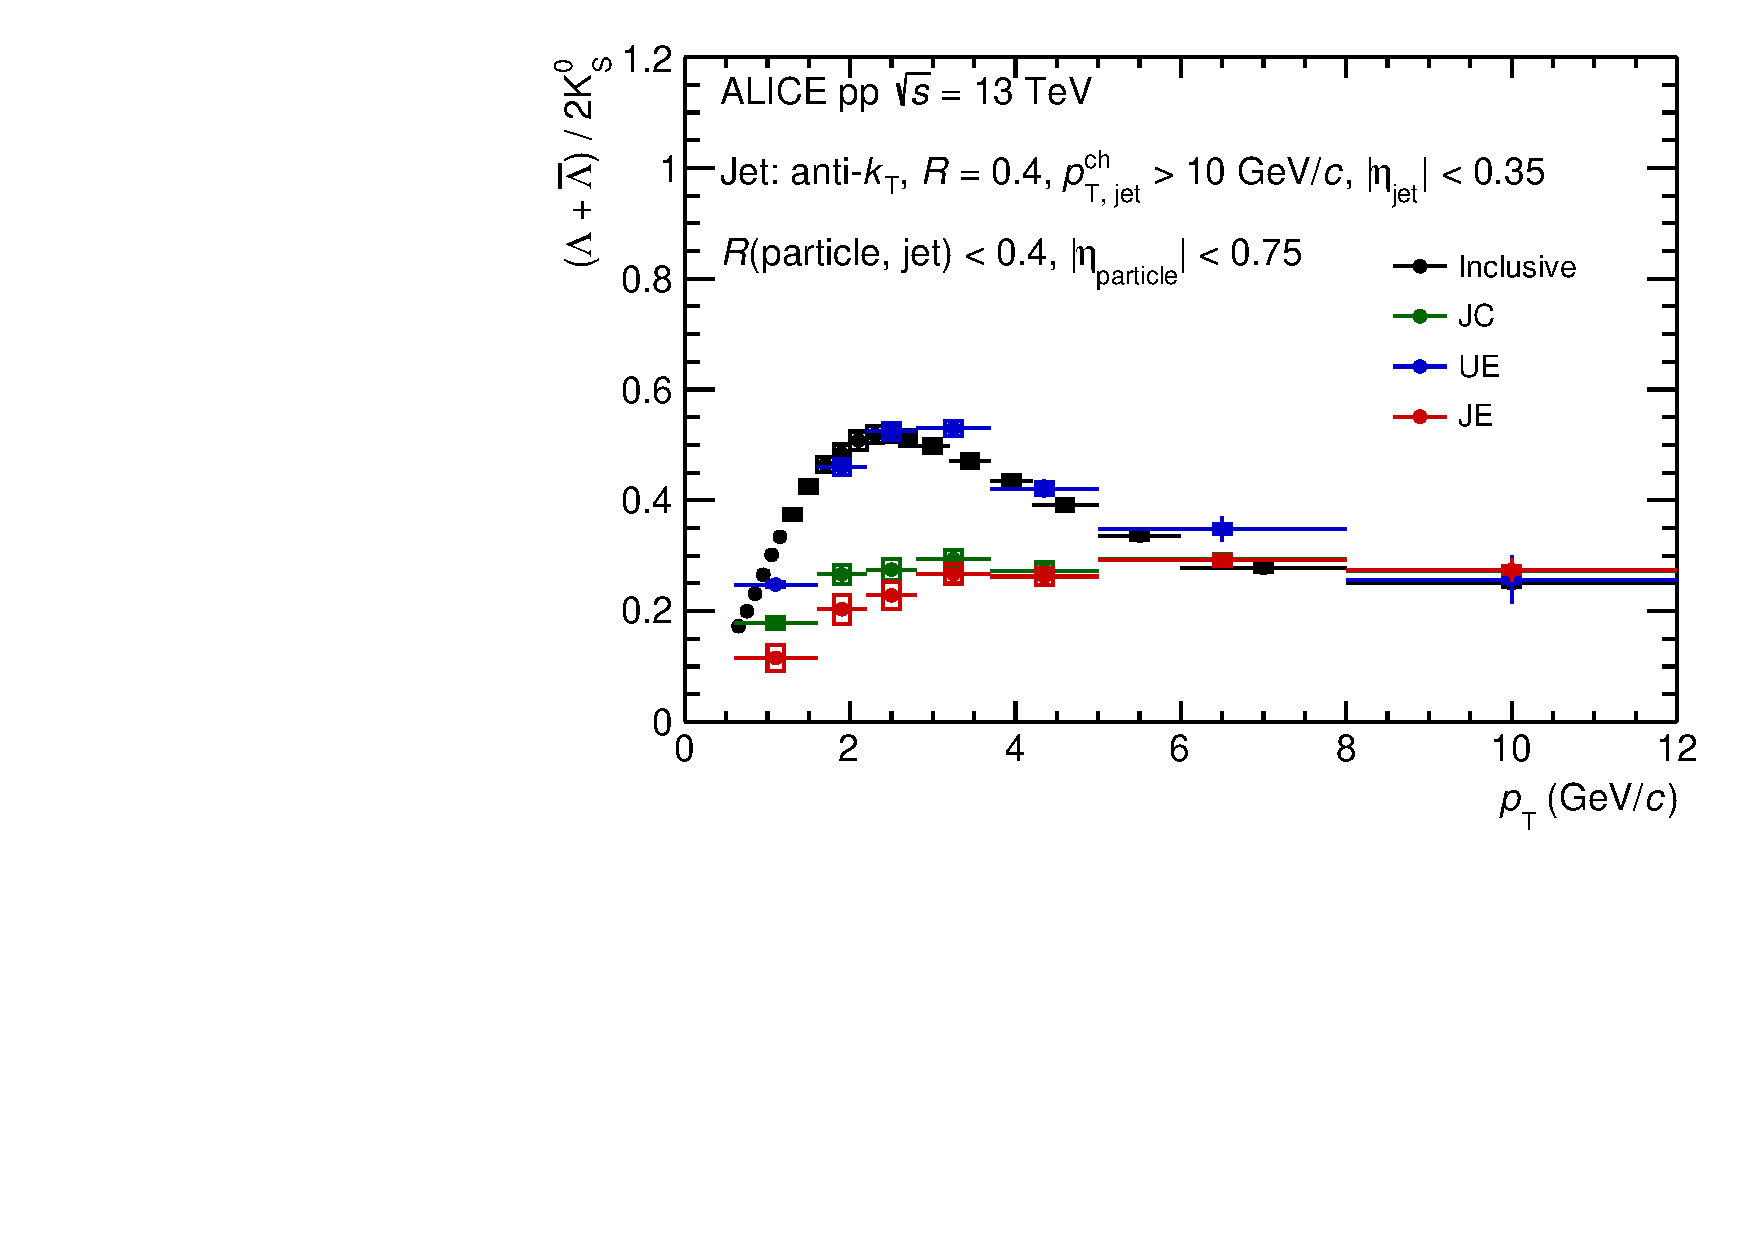
\includegraphics[width=.3\textwidth]{cf07_1}
%DIFDELCMD < 		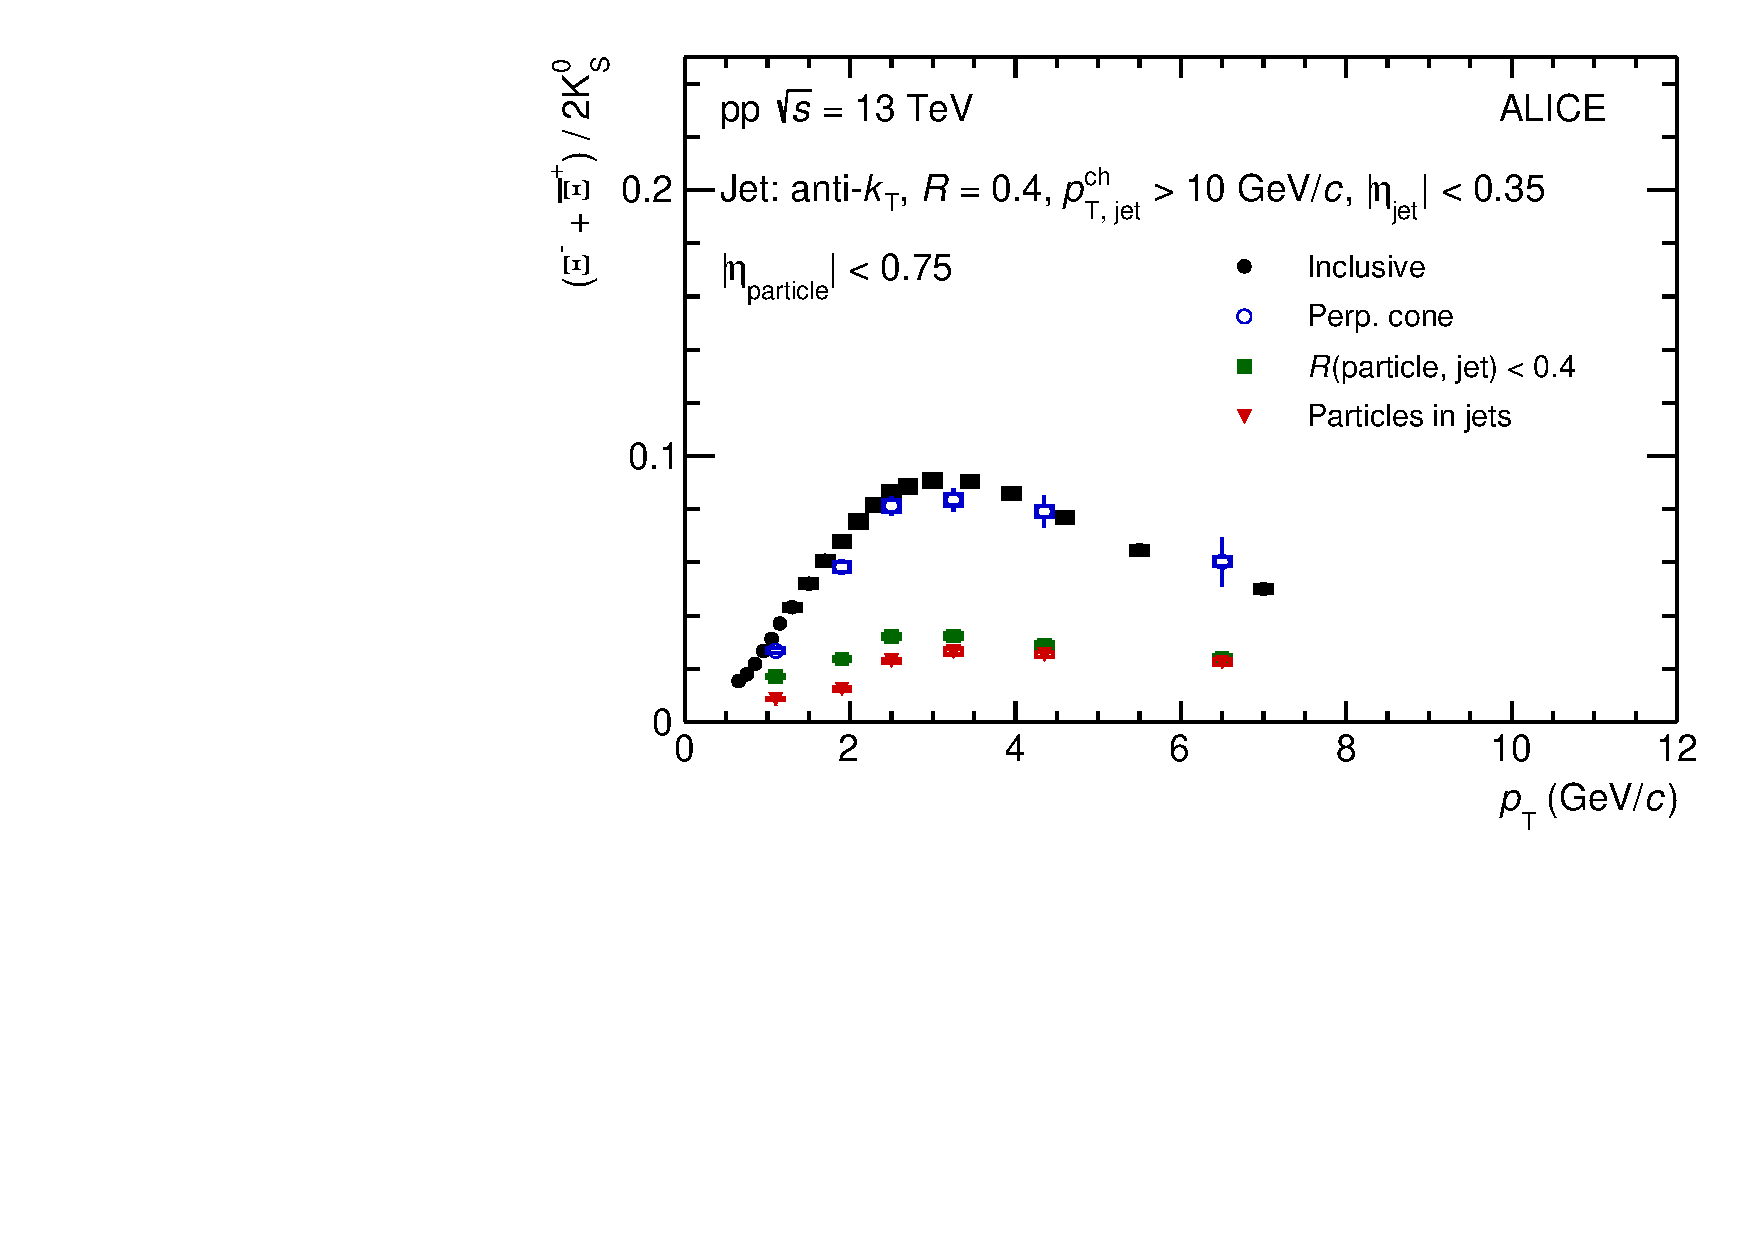
\includegraphics[width=.3\textwidth]{cf07_2}
%DIFDELCMD < 		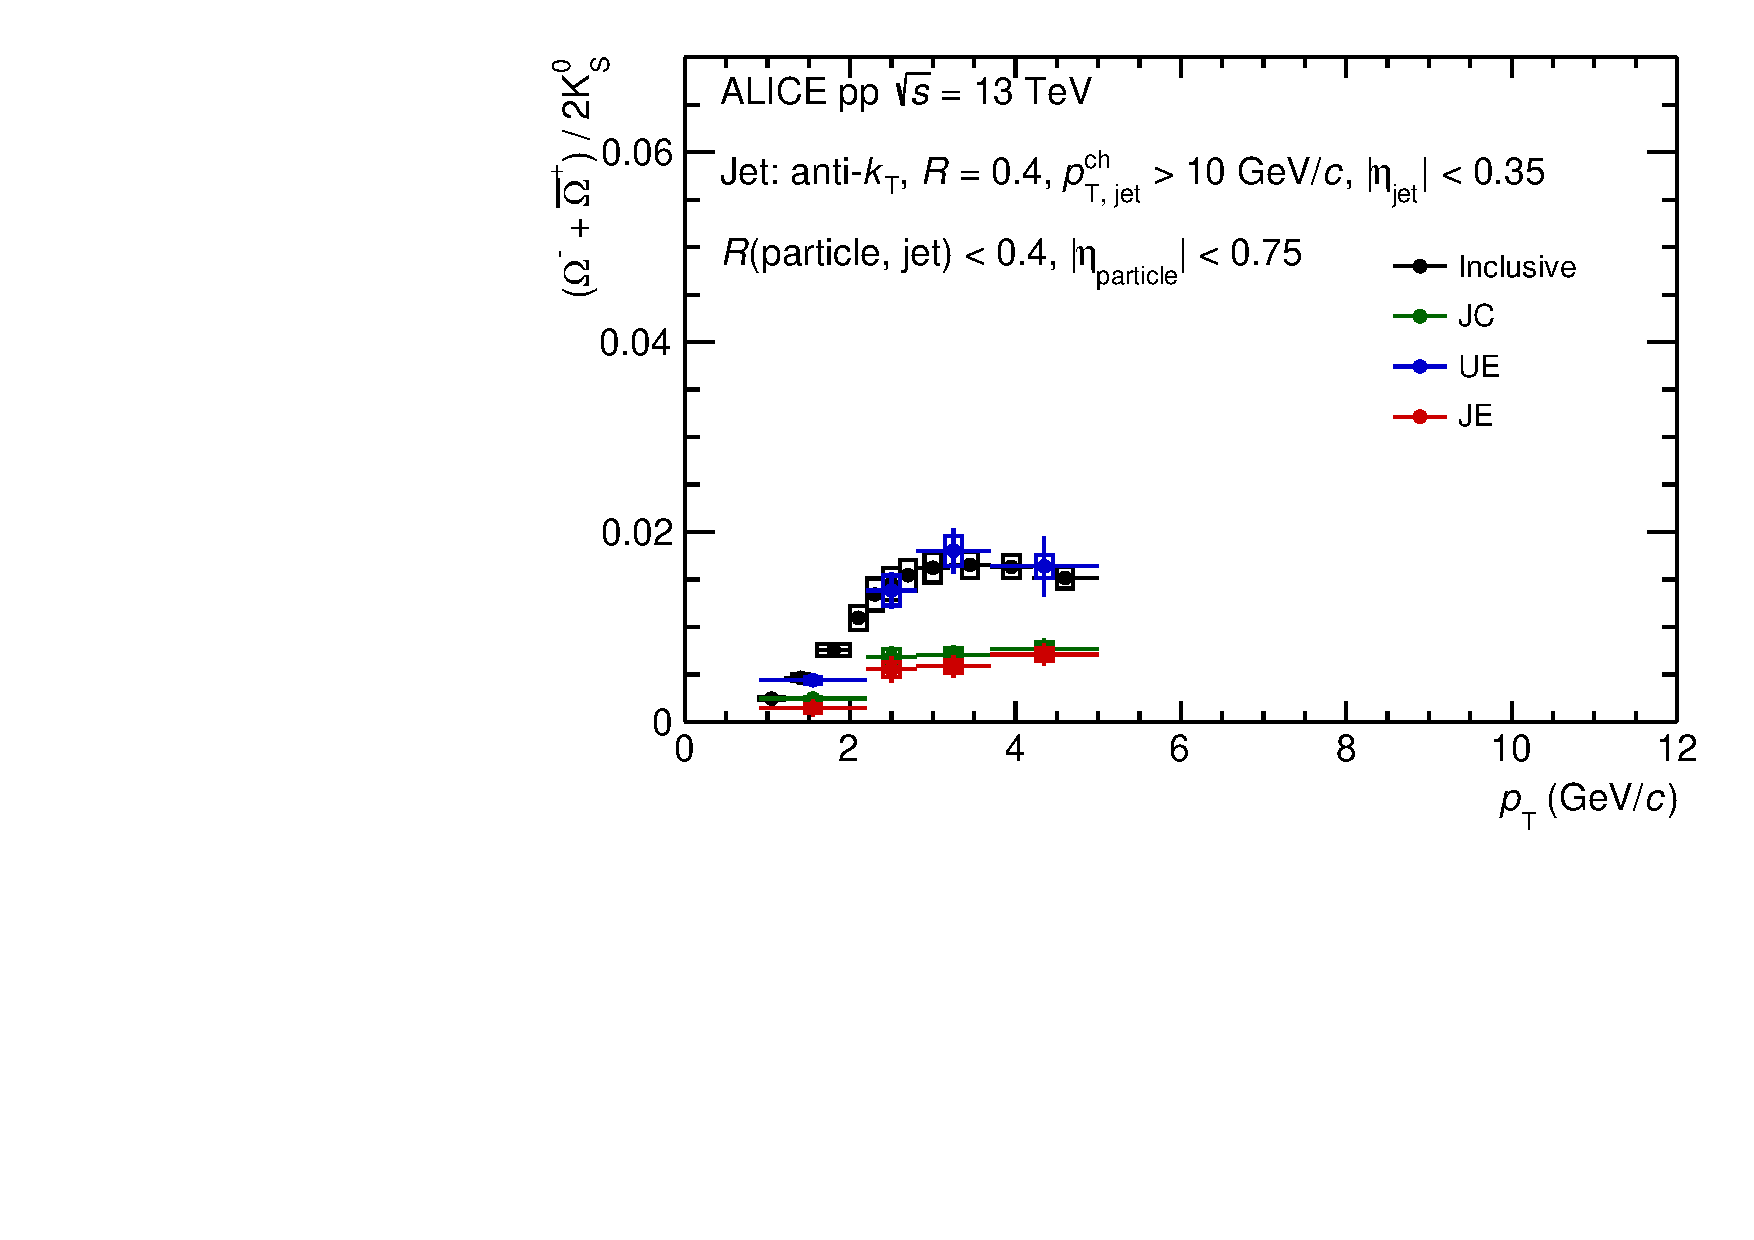
\includegraphics[width=.3\textwidth]{cf07_3}
%DIFDELCMD < 		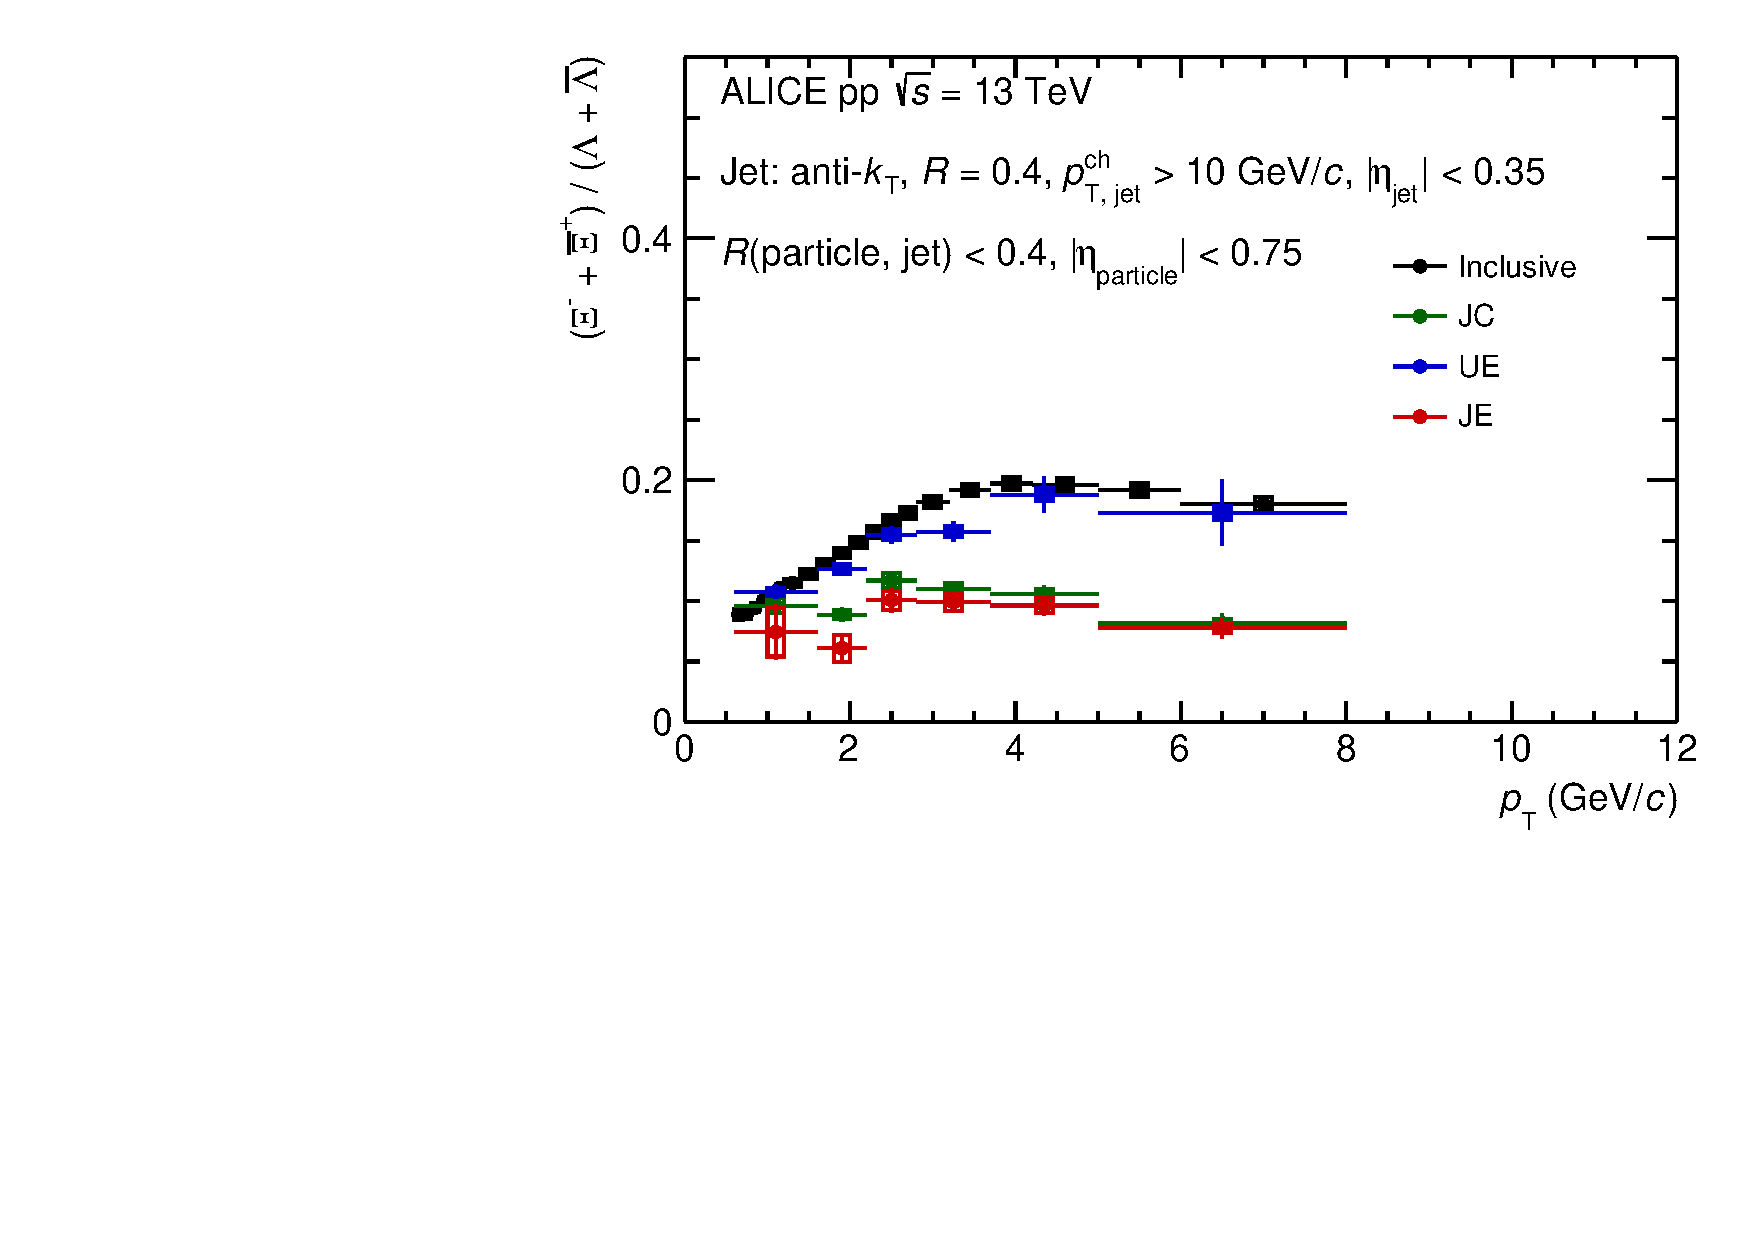
\includegraphics[width=.3\textwidth]{cf07_4}
%DIFDELCMD < 		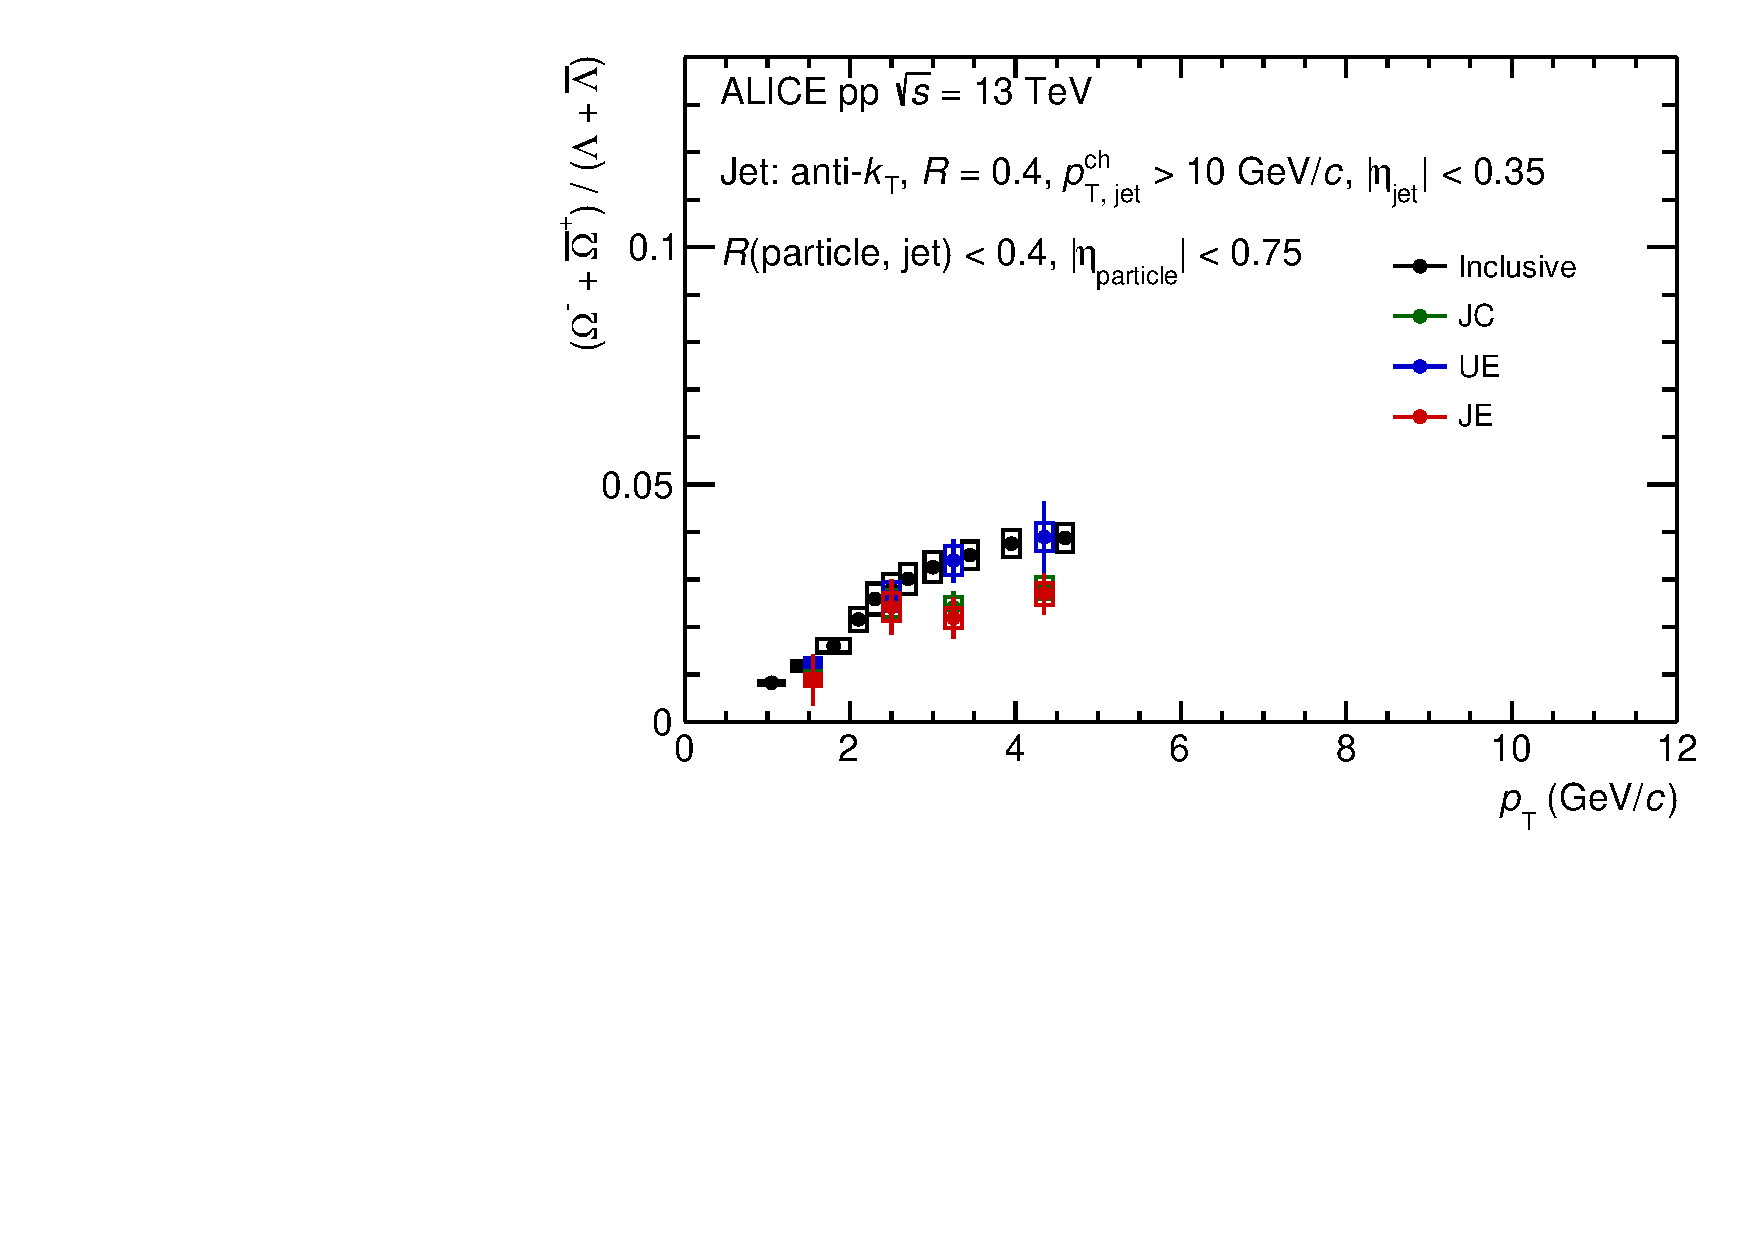
\includegraphics[width=.3\textwidth]{cf07_5}
%DIFDELCMD < 		\includegraphics[width=.3\textwidth]{cf07_6}
%DIFDELCMD < 	%%%
\DIFdelendFL \DIFaddbeginFL \includegraphics[width=.49\textwidth]{cf07_1}
		\includegraphics[width=.49\textwidth]{cf07_4}
		\includegraphics[width=.49\textwidth]{cf07_2}
		\includegraphics[width=.49\textwidth]{cf07_5}
		\includegraphics[width=.49\textwidth]{cf07_3}
		\includegraphics[width=.49\textwidth]{cf07_6}
	\DIFaddendFL \end{center}
	\caption{The baryon-to-meson (\DIFdelbeginFL \DIFdelFL{top}\DIFdelendFL \DIFaddbeginFL \DIFaddFL{left}\DIFaddendFL ) and baryon-to-baryon (\DIFdelbeginFL \DIFdelFL{bottom}\DIFdelendFL \DIFaddbeginFL \DIFaddFL{right}\DIFaddendFL ) ratio as a function of particle $\pT$ in \pp collisions at \thirteen. \DIFdelbeginFL \DIFdelFL{In those panels, the }\DIFdelendFL \DIFaddbeginFL \DIFaddFL{The }\DIFaddendFL black \DIFdelbeginFL \DIFdelFL{point shows }\DIFdelendFL \DIFaddbeginFL \DIFaddFL{points correspond to }\DIFaddendFL the ratio with particles from minimum bias events, the green \DIFdelbeginFL \DIFdelFL{point shows }\DIFdelendFL \DIFaddbeginFL \DIFaddFL{points correspond to }\DIFaddendFL the ratio with particles from the jet cones, the blue \DIFdelbeginFL \DIFdelFL{point shows }\DIFdelendFL \DIFaddbeginFL \DIFaddFL{points correspond to }\DIFaddendFL the ratio with particles \DIFdelbeginFL \DIFdelFL{from }\DIFdelendFL \DIFaddbeginFL \DIFaddFL{ratio within a cone }\DIFaddendFL perpendicular \DIFdelbeginFL \DIFdelFL{cones with }\DIFdelendFL \DIFaddbeginFL \DIFaddFL{to the }\DIFaddendFL jet\DIFaddbeginFL \DIFaddFL{, associated with the underlying event }\DIFaddendFL and the red \DIFdelbeginFL \DIFdelFL{point shows }\DIFdelendFL \DIFaddbeginFL \DIFaddFL{points represent }\DIFaddendFL the ratio \DIFdelbeginFL \DIFdelFL{with particles that generated by }\DIFdelendFL \DIFaddbeginFL \DIFaddFL{from the }\DIFaddendFL jet \DIFaddbeginFL \DIFaddFL{fragmentation. Charged-particle jets with $\pTjch > 10$~}\GeVc \DIFaddFL{were reconstructed with the }\akT \DIFaddFL{algorithm with $R = 0.4$}\DIFaddendFL .}
	\label{fig:ppRatio}
\end{figure}
\begin{figure}[!ht]
	\begin{center}
		\DIFdelbeginFL %DIFDELCMD < \includegraphics[width=.3\textwidth]{cf08_1}
%DIFDELCMD < 		\includegraphics[width=.3\textwidth]{cf08_2}
%DIFDELCMD < 		\includegraphics[width=.3\textwidth]{cf08_3}
%DIFDELCMD < 		\includegraphics[width=.3\textwidth]{cf08_4}
%DIFDELCMD < 		\includegraphics[width=.3\textwidth]{cf08_5}
%DIFDELCMD < 		\includegraphics[width=.3\textwidth]{cf08_6}
%DIFDELCMD < 	%%%
\DIFdelendFL \DIFaddbeginFL \includegraphics[width=.49\textwidth]{cf08_1}
		\includegraphics[width=.49\textwidth]{cf08_4}
		\includegraphics[width=.49\textwidth]{cf08_2}
		\includegraphics[width=.49\textwidth]{cf08_5}
		\includegraphics[width=.49\textwidth]{cf08_3}
		\includegraphics[width=.49\textwidth]{cf08_6}
	\DIFaddendFL \end{center}
	\caption{The baryon-to-meson (\DIFdelbeginFL \DIFdelFL{top}\DIFdelendFL \DIFaddbeginFL \DIFaddFL{left}\DIFaddendFL ) and baryon-to-baryon (\DIFdelbeginFL \DIFdelFL{bottom}\DIFdelendFL \DIFaddbeginFL \DIFaddFL{right}\DIFaddendFL ) ratio as a function of particle $\pT$ in \pPb collisions at \fivenn. \DIFdelbeginFL \DIFdelFL{In those panels, the }\DIFdelendFL \DIFaddbeginFL \DIFaddFL{The }\DIFaddendFL black \DIFdelbeginFL \DIFdelFL{point shows }\DIFdelendFL \DIFaddbeginFL \DIFaddFL{points correspond to }\DIFaddendFL the ratio with particles from minimum bias events, the green \DIFdelbeginFL \DIFdelFL{point shows }\DIFdelendFL \DIFaddbeginFL \DIFaddFL{points correspond to }\DIFaddendFL the ratio with particles from the jet cones, the blue \DIFdelbeginFL \DIFdelFL{point shows }\DIFdelendFL \DIFaddbeginFL \DIFaddFL{points correspond to }\DIFaddendFL the ratio with particles \DIFdelbeginFL \DIFdelFL{from }\DIFdelendFL \DIFaddbeginFL \DIFaddFL{ratio within a cone }\DIFaddendFL perpendicular \DIFdelbeginFL \DIFdelFL{cones with }\DIFdelendFL \DIFaddbeginFL \DIFaddFL{to the }\DIFaddendFL jet\DIFaddbeginFL \DIFaddFL{, associated with the underlying event }\DIFaddendFL and the red \DIFdelbeginFL \DIFdelFL{point shows }\DIFdelendFL \DIFaddbeginFL \DIFaddFL{points represent }\DIFaddendFL the ratio \DIFdelbeginFL \DIFdelFL{with particles that generated by }\DIFdelendFL \DIFaddbeginFL \DIFaddFL{from the }\DIFaddendFL jet \DIFaddbeginFL \DIFaddFL{fragmentation. Charged-particle jets with $\pTjch > 10$~}\GeVc \DIFaddFL{were reconstructed with the }\akT \DIFaddFL{algorithm with $R = 0.4$}\DIFaddendFL .}
	\label{fig:pPbRatio}
\end{figure}

\DIFdelbegin \DIFdel{The }\DIFdelend \DIFaddbegin \DIFadd{Fig.~\ref{fig:pppPbRatio} shows the }\DIFaddend particle ratios in jet \DIFdelbegin \DIFdel{with centrality and collision system distribution is studied in Fig.
~\ref{fig:pppPbRatio}}\DIFdelend \DIFaddbegin \DIFadd{in }\pp \DIFadd{collisions and in the different multiplicity classes in }\pPb \DIFadd{collisions for the same selection of the matching radius $R(\rm{particle, jet}) < 0.4$ in both systems.
The systematic uncertainties~(open boxes) are uncorrelated between the systems}\DIFaddend .
The particle ratios in the jet are observed to be relatively \DIFdelbegin \DIFdel{centrality }\DIFdelend \DIFaddbegin \DIFadd{multiplicity class }\DIFaddend and system independent.
It is noteworthy that the baryon-to-meson ($\lmb/\kzero$, $\Xi/\kzero$ and $\Omega/\kzero$) ratios have a hint of \DIFdelbegin \DIFdel{centrality }\DIFdelend \DIFaddbegin \DIFadd{multiplicity }\DIFaddend (collision system) \DIFdelbegin \DIFdel{dependent }\DIFdelend \DIFaddbegin \DIFadd{dependence }\DIFaddend for $2 < \pT < 4$~\GeVc, however \DIFdelbegin \DIFdel{this is barely significant given the quoted }\DIFdelend \DIFaddbegin \DIFadd{the difference between the ratios is less than $2\sigma$ and the measurement is currently dominated by large }\DIFaddend uncertainties.
For $\pT > 5$~\GeVc, the baryon-to-meson ratios become \DIFdelbegin \DIFdel{fairly }\DIFdelend consistent for all \DIFdelbegin \DIFdel{centrality }\DIFdelend \DIFaddbegin \DIFadd{multiplicity }\DIFaddend classes and collision systems.
\DIFaddbegin \DIFadd{In the Fig~\ref{fig:pppPbRatio}, these ratios are compared to the PYTHIA 8 simulation with Monash tune. Due to the PYTHIA overestimate with ($\X + \Ix$) (see Fig.~\ref{fig:pPbSpectwCent}) in jet spectra. So here we observed the PYTHIA can simulate the $(\lmb + \almb)/2\kzero$ well but not for the ratios which correlated with multi-strange particles.
}\DIFaddend 

\begin{figure}[!ht]
	\begin{center}
		\DIFdelbeginFL %DIFDELCMD < \includegraphics[width=.3\textwidth]{cf09_1}
%DIFDELCMD < 		\includegraphics[width=.3\textwidth]{cf09_2}
%DIFDELCMD < 		\includegraphics[width=.3\textwidth]{cf09_3}
%DIFDELCMD < 		\includegraphics[width=.3\textwidth]{cf09_4}
%DIFDELCMD < 		\includegraphics[width=.3\textwidth]{cf09_5}
%DIFDELCMD < 		\includegraphics[width=.3\textwidth]{cf09_6}
%DIFDELCMD < 	%%%
\DIFdelendFL \DIFaddbeginFL \includegraphics[width=.49\textwidth]{cf09_1}
		\includegraphics[width=.49\textwidth]{cf09_4}
		\includegraphics[width=.49\textwidth]{cf09_2}
		\includegraphics[width=.49\textwidth]{cf09_5}
		\includegraphics[width=.49\textwidth]{cf09_3}
		\includegraphics[width=.49\textwidth]{cf09_6}
	\DIFaddendFL \end{center}
	\caption{The baryon-to-meson (\DIFdelbeginFL \DIFdelFL{top}\DIFdelendFL \DIFaddbeginFL \DIFaddFL{left}\DIFaddendFL ) and baryon-to-baryon (\DIFdelbeginFL \DIFdelFL{bottom}\DIFdelendFL \DIFaddbeginFL \DIFaddFL{right}\DIFaddendFL ) \DIFdelbeginFL \DIFdelFL{ratio as a function of particle $\pT$ in jets in }\DIFdelendFL \DIFaddbeginFL \DIFaddFL{ratioin }\DIFaddendFL \pp (open symbols) \DIFaddbeginFL \DIFaddFL{collisions at }\thirteen \DIFaddendFL and \pPb (full symbols) \DIFaddbeginFL \DIFaddFL{collisions at }\fivenn \DIFaddFL{as a function of particle $\pT$ associated with charged particle jets with $\pTjch > 10$~}\GeVc \DIFaddFL{reconstructed using the }\akT \DIFaddFL{jet finder with resolution parameter $R = 0.4$. The ratios are shown for the same selection of the matching radius $R(\rm{particle, jet}) < 0.4$ in both systems}\DIFaddendFL . The different centrality classes for \pPb collisions are depicted with different color.}
	\label{fig:pppPbRatio}
\end{figure}

\DIFdelbegin %DIFDELCMD < \subsection{Comparison to models}
%DIFDELCMD < \label{subsec:ComToMod}
%DIFDELCMD < %%%
\DIFdelend %DIF > \subsection{Comparison to models}
%DIF > \label{subsec:ComToMod}

\DIFdelbegin \DIFdel{need to be added.
}\DIFdelend %DIF > need to be added.

\DIFdelbegin %DIFDELCMD < \begin{figure}[!ht]
%DIFDELCMD < 	\begin{center}
%DIFDELCMD < 		\includegraphics[width=.4\textwidth]{cf10_1}
%DIFDELCMD < 		\includegraphics[width=.4\textwidth]{cf10_2}
%DIFDELCMD < 		\includegraphics[width=.4\textwidth]{cf10_3}
%DIFDELCMD < 		\includegraphics[width=.4\textwidth]{cf10_4}
%DIFDELCMD < %%%
\DIFdelendFL %DIF > \begin{figure}[!ht]
%DIF > 	\begin{center}
%DIF > 		\includegraphics[width=.4\textwidth]{cf10_1}
%DIF > 		\includegraphics[width=.4\textwidth]{cf10_2}
%DIF > 		\includegraphics[width=.4\textwidth]{cf10_3}
%DIF > 		\includegraphics[width=.4\textwidth]{cf10_4}

\DIFdelbeginFL %DIFDELCMD < \end{center}
%DIFDELCMD < 	%%%
%DIFDELCMD < \caption{%
{%DIFAUXCMD
\DIFdelFL{Particles in jet in }%DIFDELCMD < \pPb %%%
\DIFdelFL{at }%DIFDELCMD < \fivenn %%%
\DIFdelFL{with PYTHIA 8 BLC mode 0}}
	%DIFAUXCMD
%DIFDELCMD < \label{fig:pPbpyJESpect}
%DIFDELCMD < \end{figure}
%DIFDELCMD < %%%
\DIFdelend %DIF > 	\end{center}
%DIF > 	\caption{Particles in jet in \pPb at \fivenn with PYTHIA 8 BLC mode 0}
%DIF > 	\label{fig:pPbpyJESpect}
%DIF > \end{figure}


\clearpage
\section{Summary}%
\label{sec:Summary}

\DIFdelbegin \DIFdel{We studied }\DIFdelend \DIFaddbegin \DIFadd{The first measurement of }\DIFaddend the \kzero, \lmb (\almb), \Xis and \Oms $\pT$-differential density, the $\lmb/\kzero$, $\Xi/\kzero$ and $\Omega/\kzero$ baryon-to-meson ratio and the $\Xi/\lmb$, $\Omega/\lmb$ and $\Omega/\Xi$ baryon-to-baryon ratio in \DIFaddbegin \DIFadd{charged-particle }\DIFaddend jets and underlying events in \pp \DIFaddbegin \DIFadd{collisions }\DIFaddend at \thirteen and \pPb \DIFaddbegin \DIFadd{collisions }\DIFaddend at \fivenn \DIFdelbegin \DIFdel{collisions}\DIFdelend \DIFaddbegin \DIFadd{have been studied.
All the measured quantities are compared with PYTHIA 8 model predictions.
The PYTHIA 8 with the standard Monash trigg tune can describe the $\kzero, \lmb + \almb$, but not for the $\X + \Ix$ and $\Om + \Mo$}\DIFaddend .
The main \DIFdelbegin \DIFdel{feature of this analysis is the usage of charged particle }\DIFdelend \DIFaddbegin \DIFadd{aim of the presented analysis, based on charged-particle }\DIFaddend jet to separate hard and soft \DIFdelbegin \DIFdel{progress, providing new }\DIFdelend \DIFaddbegin \DIFadd{process, is to provide }\DIFaddend insight into the understanding of the origin of flow-like correlations observed in small systems.

\DIFdelbegin \DIFdel{The }\DIFdelend \DIFaddbegin \DIFadd{For all particle the }\DIFaddend $\pT$-differential density in events with charged-particle jet ($\pTjch$ > 10~\GeVc) are observed to \DIFdelbegin \DIFdel{become }\DIFdelend \DIFaddbegin \DIFadd{be }\DIFaddend harder than that in MB events.
\DIFdelbegin \DIFdel{Also}\DIFdelend \DIFaddbegin \DIFadd{In addition}\DIFaddend , the dependence on charged-particle multiplicity found in the inclusive particle is not present for particles generated by jet fragmentation.
\DIFdelbegin %DIFDELCMD < 

%DIFDELCMD < %%%
\DIFdelend \DIFaddbegin \DIFadd{The baryon-to-meson and baryon-to-baryon ratios associated with jets in }\pPb \DIFadd{collisions for $R({\rm particle, jet} < 0.4)$ is consistent with the ratio measured in }\pp \DIFadd{collisions.
The ratios are observed to be independent on the multiplicity class of }\pPb \DIFadd{collisions.
}\DIFaddend The enhancement of \DIFdelbegin \DIFdel{baron-to-meson }\DIFdelend \DIFaddbegin \DIFadd{baryon-to-meson }\DIFaddend ratio at intermediate $\pT$ found in the inclusive particle \DIFdelbegin \DIFdel{in }%DIFDELCMD < \pp %%%
\DIFdel{and }%DIFDELCMD < \pPb %%%
\DIFdel{collisions }\DIFdelend are not present for particles associated with hard scattering \DIFdelbegin \DIFdel{.
}%DIFDELCMD < \emp{to be finished}
%DIFDELCMD < %%%
\DIFdelend \DIFaddbegin \DIFadd{tagged by jets reconstructed from charged particles for $\pTjch > 10$~}\GeVc \DIFadd{in }\pp \DIFadd{and }\pPb \DIFadd{collisions.
Moreover, as the baryon-to-meson enhancement has been linked to the interplay of radial flow and parton recombination at intermediate $\pT$, its absence within the jet cone demonstrates that these effects are indeed limited to the soft particle production process.
}

\DIFaddend %==========================================

\newenvironment{acknowledgement}{\relax}{\relax}
\begin{acknowledgement}
\section*{Acknowledgements}
%\input{acknowledgements.tex}

\end{acknowledgement}

\bibliographystyle{etc/utphys}
\bibliography{AliStrangeJets}

\newpage
\appendix
%\input{} % put your appendices here (if any)
\DIFaddbegin \section{Particle candidate selection criteria}
\begin{table}[!ht]
	\begin{center}
		\caption{\kzero\DIFaddFL{(}\lmb \DIFaddFL{and }\almb\DIFaddFL{) candidate selection criteria of topological variables, daughter tracks and }\Vzero \DIFaddFL{candidates.
			The DCA stands for the ``Distance of Closest Approach'', PV represents the ``Primary collision Vertex'' and CPA is the ``Cosine Pointing Angle between the momentum vector of the reconstructed }\Vzero \DIFaddFL{and the displacement vector between the decay and primary vertices''.}}
		\label{tab:V0Cut}
		\begin{tabularx}{\textwidth}{@{} lCC @{}}
			\toprule
			\textbf{\DIFaddFL{Topological variable}} & \textbf{\pp} & \textbf{\pPb} \\
			\midrule
			\DIFaddFL{$\Vzero$ transverse decay radius      }& \DIFaddFL{$> 0.5$~cm   }& \DIFaddFL{$> 0.5$~cm }\\
			\DIFaddFL{DCA of positive / negative track to PV }& \DIFaddFL{$> 0.06$~cm  }& \DIFaddFL{$> 0.06$~cm }\\
			\DIFaddFL{DCA between $\Vzero$ daughter tracks  }& \DIFaddFL{$< 1.0\sigma$ }& \DIFaddFL{$< 1\sigma$ }\\
			\DIFaddFL{CPA of $\Vzero$ }& \DIFaddFL{$> 0.97$ ($0.995$) }& \DIFaddFL{$> 0.97$ ($0.995$) }\\
			\midrule
			\textbf{\DIFaddFL{Track selection}} \\
			\midrule
			\DIFaddFL{Daughter track pseudo-rapidity interval }&\DIFaddFL{$|\eta| < 0.8$ }& \DIFaddFL{$\abs{\eta} < 0.8$      }\\
			\DIFaddFL{Daughter track $N_{\rm crossed~rows}$                   }& \DIFaddFL{$\geq 70$  }& \DIFaddFL{$\geq$ 70 }\\
			\DIFaddFL{Daughter Track $N_{\rm crossed~rows}/N_{\rm findable}$  }& \DIFaddFL{$\geq 0.8$ }& \DIFaddFL{$\geq$ 0.8 }\\
			\DIFaddFL{TPC $\dEdx$ }& \DIFaddFL{$< 5\sigma$ }& \DIFaddFL{$< 5\sigma$ }\\
			\midrule
			\textbf{\DIFaddFL{Candidate selection}} \\
			\midrule
			\DIFaddFL{Pseudo-rapidity interval }& \DIFaddFL{$|\eta| < 0.75$ }& \DIFaddFL{$|\eta| < 0.75$ }\\
			\DIFaddFL{Proper lifetime($mL/p$)  }& \DIFaddFL{$< 20$ (30)~cm }& \DIFaddFL{$< 20$ (30)~cm }\\
			\DIFaddFL{Competing mass }& \DIFaddFL{$> 0.005$ (0.010)~}\GeVmass & \DIFaddFL{$> 0.005$ (0.010)~}\GeVmass \\
			\bottomrule
		\end{tabularx}
	\end{center}
\end{table}
\DIFaddend 

\DIFaddbegin \begin{table}[!ht]
	\begin{center}
		\caption{\Xis\DIFaddFL{(}\Oms\DIFaddFL{) candidate selection criteria of topological variables, daughter tracks and cascade candidates.}}
		\label{tab:CascadeCut}
		\begin{tabularx}{\textwidth}{@{} lCC @{}}
			\toprule
			\textbf{\DIFaddFL{Topological variable}} & \textbf{\pp} & \textbf{\pPb} \\
			\midrule
			\DIFaddFL{Cascade transverse decay radius }& \DIFaddFL{$> 0.8(0.6)$~cm }& \DIFaddFL{$> 0.6$~cm }\\
			\Vzero \DIFaddFL{transverse decay radius }& \DIFaddFL{$> 1.4$~cm     }& \DIFaddFL{$> 1.2$~cm }\\
			\DIFaddFL{DCA (bachelor to PV)           }& \DIFaddFL{$> 0.05$~cm    }& \DIFaddFL{$> 0.04$~cm }\\
			\DIFaddFL{DCA (}\Vzero \DIFaddFL{to PV)             }& \DIFaddFL{$> 0.07$~cm    }& \DIFaddFL{$> 0.06$~cm }\\
			\DIFaddFL{DCA (positive / negative track to PV) }& \DIFaddFL{$> 0.04(0.03)$~cm }& \DIFaddFL{$> 0.03$~cm  }\\
			\DIFaddFL{DCA between }\Vzero \DIFaddFL{daughter tracks }& \DIFaddFL{$< 1.6\sigma$     }& \DIFaddFL{$< 1.5\sigma$ }\\
			\DIFaddFL{DCA (bachelor to }\Vzero\DIFaddFL{) }& \DIFaddFL{$< 1.6(1.0)$~cm }& \DIFaddFL{$< 1.3$~cm }\\
			\DIFaddFL{CPA of Cascade          }& \DIFaddFL{$> 0.97$       }& \DIFaddFL{$> 0.97$  }\\
			\DIFaddFL{CPA of }\Vzero           & \DIFaddFL{$> 0.97$       }& \DIFaddFL{$> 0.97$  }\\
			\Vzero \DIFaddFL{invariant mass window }& \DIFaddFL{$\pm 0.006$~}\GeVmass & \DIFaddFL{$\pm 0.008$~}\GeVmass \\
			\midrule
			\textbf{\DIFaddFL{Track selection}} \\
			\midrule
			\DIFaddFL{Daughter track pseudo-rapidity interval }& \DIFaddFL{$|\eta| < 0.8$ }& \DIFaddFL{$|\eta| < 0.8$ }\\
			\DIFaddFL{Daughter track $N_{\rm crossed~rows}$  }& \DIFaddFL{$\geq 70$      }& \DIFaddFL{$\geq$ 70 }\\
			\DIFaddFL{Daughter Track $N_{\rm crossed~rows}/N_{\rm findable}$ }&\DIFaddFL{$\geq 0.8$ }&\DIFaddFL{$\geq$ 0.8 }\\
			\DIFaddFL{TPC $\dEdx$ }& \DIFaddFL{$< 5\sigma$ }& \DIFaddFL{$< 4\sigma$ }\\
			\midrule
			\textbf{\DIFaddFL{Candidate selection}} \\
			\midrule
			\DIFaddFL{Pseudo-rapidity interval }& \DIFaddFL{$|\eta| < 0.75$ }&\DIFaddFL{$|\eta| < 0.75$ }\\
			\DIFaddFL{Proper lifetime ($mL/p$) }& & \DIFaddFL{$< 3 \times c\tau$ }\\
			\DIFaddFL{Competing mass          }& \DIFaddFL{$8$~}\MeVmass & \DIFaddFL{$8$~}\MeVmass \\
			\bottomrule
		\end{tabularx}
	\end{center}
\end{table}
\DIFaddend \section{The ALICE Collaboration}
\label{app:collab}
%\input{authorlist-preprint.tex}  
\end{document}
